\documentclass[twoside]{book}

% Packages required by doxygen
\usepackage{calc}
\usepackage{doxygen}
\usepackage{graphicx}
\usepackage[utf8]{inputenc}
\usepackage{makeidx}
\usepackage{multicol}
\usepackage{multirow}
\usepackage{textcomp}
\usepackage[table]{xcolor}

% Font selection
\usepackage[T1]{fontenc}
\usepackage{mathptmx}
\usepackage[scaled=.90]{helvet}
\usepackage{courier}
\usepackage{amssymb}
\usepackage{sectsty}
\renewcommand{\familydefault}{\sfdefault}
\allsectionsfont{%
  \fontseries{bc}\selectfont%
  \color{darkgray}%
}
\renewcommand{\DoxyLabelFont}{%
  \fontseries{bc}\selectfont%
  \color{darkgray}%
}

% Page & text layout
\usepackage{geometry}
\geometry{%
  a4paper,%
  top=2.5cm,%
  bottom=2.5cm,%
  left=2.5cm,%
  right=2.5cm%
}
\tolerance=750
\hfuzz=15pt
\hbadness=750
\setlength{\emergencystretch}{15pt}
\setlength{\parindent}{0cm}
\setlength{\parskip}{0.2cm}
\makeatletter
\renewcommand{\paragraph}{%
  \@startsection{paragraph}{4}{0ex}{-1.0ex}{1.0ex}{%
    \normalfont\normalsize\bfseries\SS@parafont%
  }%
}
\renewcommand{\subparagraph}{%
  \@startsection{subparagraph}{5}{0ex}{-1.0ex}{1.0ex}{%
    \normalfont\normalsize\bfseries\SS@subparafont%
  }%
}
\makeatother

% Headers & footers
\usepackage{fancyhdr}
\pagestyle{fancyplain}
\fancyhead[LE]{\fancyplain{}{\bfseries\thepage}}
\fancyhead[CE]{\fancyplain{}{}}
\fancyhead[RE]{\fancyplain{}{\bfseries\leftmark}}
\fancyhead[LO]{\fancyplain{}{\bfseries\rightmark}}
\fancyhead[CO]{\fancyplain{}{}}
\fancyhead[RO]{\fancyplain{}{\bfseries\thepage}}
\fancyfoot[LE]{\fancyplain{}{}}
\fancyfoot[CE]{\fancyplain{}{}}
\fancyfoot[RE]{\fancyplain{}{\bfseries\scriptsize Generated on Mon Sep 28 2015 13\-:20\-:08 for My Project by Doxygen }}
\fancyfoot[LO]{\fancyplain{}{\bfseries\scriptsize Generated on Mon Sep 28 2015 13\-:20\-:08 for My Project by Doxygen }}
\fancyfoot[CO]{\fancyplain{}{}}
\fancyfoot[RO]{\fancyplain{}{}}
\renewcommand{\footrulewidth}{0.4pt}
\renewcommand{\chaptermark}[1]{%
  \markboth{#1}{}%
}
\renewcommand{\sectionmark}[1]{%
  \markright{\thesection\ #1}%
}

% Indices & bibliography
\usepackage{natbib}
\usepackage[titles]{tocloft}
\setcounter{tocdepth}{3}
\setcounter{secnumdepth}{5}
\makeindex

% Hyperlinks (required, but should be loaded last)
\usepackage{ifpdf}
\ifpdf
  \usepackage[pdftex,pagebackref=true]{hyperref}
\else
  \usepackage[ps2pdf,pagebackref=true]{hyperref}
\fi
\hypersetup{%
  colorlinks=true,%
  linkcolor=blue,%
  citecolor=blue,%
  unicode%
}

% Custom commands
\newcommand{\clearemptydoublepage}{%
  \newpage{\pagestyle{empty}\cleardoublepage}%
}


%===== C O N T E N T S =====

\begin{document}

% Titlepage & ToC
\hypersetup{pageanchor=false}
\pagenumbering{roman}
\begin{titlepage}
\vspace*{7cm}
\begin{center}%
{\Large My Project }\\
\vspace*{1cm}
{\large Generated by Doxygen 1.8.6}\\
\vspace*{0.5cm}
{\small Mon Sep 28 2015 13:20:08}\\
\end{center}
\end{titlepage}
\clearemptydoublepage
\tableofcontents
\clearemptydoublepage
\pagenumbering{arabic}
\hypersetup{pageanchor=true}

%--- Begin generated contents ---
\chapter{Hierarchical Index}
\section{Class Hierarchy}
This inheritance list is sorted roughly, but not completely, alphabetically\-:\begin{DoxyCompactList}
\item \contentsline{section}{bounds}{\pageref{structbounds}}{}
\begin{DoxyCompactList}
\item \contentsline{section}{var}{\pageref{structvar}}{}
\end{DoxyCompactList}
\item \contentsline{section}{B\-P\-\_\-\-Input}{\pageref{class_b_p___input}}{}
\item \contentsline{section}{B\-P\-\_\-\-Output}{\pageref{class_b_p___output}}{}
\item \contentsline{section}{Clock}{\pageref{class_clock}}{}
\item \contentsline{section}{Constraint}{\pageref{class_constraint}}{}
\begin{DoxyCompactList}
\item \contentsline{section}{Linear}{\pageref{class_linear}}{}
\end{DoxyCompactList}
\item \contentsline{section}{Constraint\-Sorter}{\pageref{class_constraint_sorter}}{}
\item \contentsline{section}{elem}{\pageref{structelem}}{}
\item \contentsline{section}{General\-Solver}{\pageref{class_general_solver}}{}
\begin{DoxyCompactList}
\item \contentsline{section}{B\-P\-Solver}{\pageref{class_b_p_solver}}{}
\end{DoxyCompactList}
\item \contentsline{section}{Integer\-Variable}{\pageref{class_integer_variable}}{}
\item \contentsline{section}{Invariant}{\pageref{class_invariant}}{}
\begin{DoxyCompactList}
\item \contentsline{section}{Sum}{\pageref{class_sum}}{}
\end{DoxyCompactList}
\item \contentsline{section}{L\-S\-Space}{\pageref{class_l_s_space}}{}
\item \contentsline{section}{Model}{\pageref{class_model}}{}
\item \contentsline{section}{Move}{\pageref{class_move}}{}
\begin{DoxyCompactList}
\item \contentsline{section}{Flip\-Move}{\pageref{class_flip_move}}{}
\item \contentsline{section}{Value\-Change\-Move}{\pageref{class_value_change_move}}{}
\end{DoxyCompactList}
\item \contentsline{section}{Neighborhood\-Explorer}{\pageref{class_neighborhood_explorer}}{}
\item \contentsline{section}{Options}{\pageref{class_options}}{}
\item \contentsline{section}{Random}{\pageref{class_random}}{}
\item \contentsline{section}{Constraint\-:\-:Sort\-Greater}{\pageref{struct_constraint_1_1_sort_greater}}{}
\item Space\begin{DoxyCompactList}
\item \contentsline{section}{Gecode\-Solver}{\pageref{class_gecode_solver}}{}
\end{DoxyCompactList}
\item \contentsline{section}{State}{\pageref{class_state}}{}
\item Stop\begin{DoxyCompactList}
\item \contentsline{section}{Multistop}{\pageref{class_multistop}}{}
\end{DoxyCompactList}
\end{DoxyCompactList}

\chapter{Class Index}
\section{Class List}
Here are the classes, structs, unions and interfaces with brief descriptions\-:\begin{DoxyCompactList}
\item\contentsline{section}{\hyperlink{structbounds}{bounds} }{\pageref{structbounds}}{}
\item\contentsline{section}{\hyperlink{class_b_p___input}{B\-P\-\_\-\-Input} }{\pageref{class_b_p___input}}{}
\item\contentsline{section}{\hyperlink{class_b_p___output}{B\-P\-\_\-\-Output} }{\pageref{class_b_p___output}}{}
\item\contentsline{section}{\hyperlink{class_b_p_solver}{B\-P\-Solver} }{\pageref{class_b_p_solver}}{}
\item\contentsline{section}{\hyperlink{class_clock}{Clock} }{\pageref{class_clock}}{}
\item\contentsline{section}{\hyperlink{class_constraint}{Constraint} }{\pageref{class_constraint}}{}
\item\contentsline{section}{\hyperlink{class_constraint_sorter}{Constraint\-Sorter} }{\pageref{class_constraint_sorter}}{}
\item\contentsline{section}{\hyperlink{structelem}{elem} }{\pageref{structelem}}{}
\item\contentsline{section}{\hyperlink{class_flip_move}{Flip\-Move} }{\pageref{class_flip_move}}{}
\item\contentsline{section}{\hyperlink{class_gecode_solver}{Gecode\-Solver} }{\pageref{class_gecode_solver}}{}
\item\contentsline{section}{\hyperlink{class_general_solver}{General\-Solver} }{\pageref{class_general_solver}}{}
\item\contentsline{section}{\hyperlink{class_integer_variable}{Integer\-Variable} }{\pageref{class_integer_variable}}{}
\item\contentsline{section}{\hyperlink{class_invariant}{Invariant} }{\pageref{class_invariant}}{}
\item\contentsline{section}{\hyperlink{class_linear}{Linear} }{\pageref{class_linear}}{}
\item\contentsline{section}{\hyperlink{class_l_s_space}{L\-S\-Space} }{\pageref{class_l_s_space}}{}
\item\contentsline{section}{\hyperlink{class_model}{Model} }{\pageref{class_model}}{}
\item\contentsline{section}{\hyperlink{class_move}{Move} }{\pageref{class_move}}{}
\item\contentsline{section}{\hyperlink{class_multistop}{Multistop} }{\pageref{class_multistop}}{}
\item\contentsline{section}{\hyperlink{class_neighborhood_explorer}{Neighborhood\-Explorer} }{\pageref{class_neighborhood_explorer}}{}
\item\contentsline{section}{\hyperlink{class_options}{Options} }{\pageref{class_options}}{}
\item\contentsline{section}{\hyperlink{class_random}{Random} }{\pageref{class_random}}{}
\item\contentsline{section}{\hyperlink{struct_constraint_1_1_sort_greater}{Constraint\-::\-Sort\-Greater} }{\pageref{struct_constraint_1_1_sort_greater}}{}
\item\contentsline{section}{\hyperlink{class_state}{State} }{\pageref{class_state}}{}
\item\contentsline{section}{\hyperlink{class_sum}{Sum} }{\pageref{class_sum}}{}
\item\contentsline{section}{\hyperlink{class_value_change_move}{Value\-Change\-Move} }{\pageref{class_value_change_move}}{}
\item\contentsline{section}{\hyperlink{structvar}{var} }{\pageref{structvar}}{}
\end{DoxyCompactList}

\chapter{File Index}
\section{File List}
Here is a list of all files with brief descriptions\-:\begin{DoxyCompactList}
\item\contentsline{section}{\hyperlink{_b_p___data_8cpp}{B\-P\-\_\-\-Data.\-cpp} }{\pageref{_b_p___data_8cpp}}{}
\item\contentsline{section}{\hyperlink{_b_p___data_8hpp}{B\-P\-\_\-\-Data.\-hpp} }{\pageref{_b_p___data_8hpp}}{}
\item\contentsline{section}{\hyperlink{_b_p_solver_8hpp}{B\-P\-Solver.\-hpp} }{\pageref{_b_p_solver_8hpp}}{}
\item\contentsline{section}{\hyperlink{_clock_8cpp}{Clock.\-cpp} }{\pageref{_clock_8cpp}}{}
\item\contentsline{section}{\hyperlink{_clock_8hpp}{Clock.\-hpp} }{\pageref{_clock_8hpp}}{}
\item\contentsline{section}{\hyperlink{_constants_8hpp}{Constants.\-hpp} }{\pageref{_constants_8hpp}}{}
\item\contentsline{section}{\hyperlink{_constraint_8hpp}{Constraint.\-hpp} }{\pageref{_constraint_8hpp}}{}
\item\contentsline{section}{\hyperlink{_flip_move_8cpp}{Flip\-Move.\-cpp} }{\pageref{_flip_move_8cpp}}{}
\item\contentsline{section}{\hyperlink{_flip_move_8hpp}{Flip\-Move.\-hpp} }{\pageref{_flip_move_8hpp}}{}
\item\contentsline{section}{\hyperlink{_gecode_solver_8cpp}{Gecode\-Solver.\-cpp} }{\pageref{_gecode_solver_8cpp}}{}
\item\contentsline{section}{\hyperlink{_gecode_solver_8hpp}{Gecode\-Solver.\-hpp} }{\pageref{_gecode_solver_8hpp}}{}
\item\contentsline{section}{\hyperlink{_general_solver_8cpp}{General\-Solver.\-cpp} }{\pageref{_general_solver_8cpp}}{}
\item\contentsline{section}{\hyperlink{_general_solver_8hpp}{General\-Solver.\-hpp} }{\pageref{_general_solver_8hpp}}{}
\item\contentsline{section}{\hyperlink{get_r_s_s_8hpp}{get\-R\-S\-S.\-hpp} }{\pageref{get_r_s_s_8hpp}}{}
\item\contentsline{section}{\hyperlink{_integer_variable_8cpp}{Integer\-Variable.\-cpp} }{\pageref{_integer_variable_8cpp}}{}
\item\contentsline{section}{\hyperlink{_integer_variable_8hpp}{Integer\-Variable.\-hpp} }{\pageref{_integer_variable_8hpp}}{}
\item\contentsline{section}{\hyperlink{_invariant_8hpp}{Invariant.\-hpp} }{\pageref{_invariant_8hpp}}{}
\item\contentsline{section}{\hyperlink{_linear_8hpp}{Linear.\-hpp} }{\pageref{_linear_8hpp}}{}
\item\contentsline{section}{\hyperlink{_l_s_space_8cpp}{L\-S\-Space.\-cpp} }{\pageref{_l_s_space_8cpp}}{}
\item\contentsline{section}{\hyperlink{_l_s_space_8hpp}{L\-S\-Space.\-hpp} }{\pageref{_l_s_space_8hpp}}{}
\item\contentsline{section}{\hyperlink{main_8cpp}{main.\-cpp} }{\pageref{main_8cpp}}{}
\item\contentsline{section}{\hyperlink{_model_8cpp}{Model.\-cpp} }{\pageref{_model_8cpp}}{}
\item\contentsline{section}{\hyperlink{_model_8hpp}{Model.\-hpp} }{\pageref{_model_8hpp}}{}
\item\contentsline{section}{\hyperlink{_move_8hpp}{Move.\-hpp} }{\pageref{_move_8hpp}}{}
\item\contentsline{section}{\hyperlink{_multistop_8cpp}{Multistop.\-cpp} }{\pageref{_multistop_8cpp}}{}
\item\contentsline{section}{\hyperlink{_multistop_8hpp}{Multistop.\-hpp} }{\pageref{_multistop_8hpp}}{}
\item\contentsline{section}{\hyperlink{_neighborhood_explorer_8cpp}{Neighborhood\-Explorer.\-cpp} }{\pageref{_neighborhood_explorer_8cpp}}{}
\item\contentsline{section}{\hyperlink{_neighborhood_explorer_8hpp}{Neighborhood\-Explorer.\-hpp} }{\pageref{_neighborhood_explorer_8hpp}}{}
\item\contentsline{section}{\hyperlink{_options_8cpp}{Options.\-cpp} }{\pageref{_options_8cpp}}{}
\item\contentsline{section}{\hyperlink{_options_8hpp}{Options.\-hpp} }{\pageref{_options_8hpp}}{}
\item\contentsline{section}{\hyperlink{_random_8cpp}{Random.\-cpp} }{\pageref{_random_8cpp}}{}
\item\contentsline{section}{\hyperlink{_random_8hpp}{Random.\-hpp} }{\pageref{_random_8hpp}}{}
\item\contentsline{section}{\hyperlink{_state_8cpp}{State.\-cpp} }{\pageref{_state_8cpp}}{}
\item\contentsline{section}{\hyperlink{_state_8hpp}{State.\-hpp} }{\pageref{_state_8hpp}}{}
\item\contentsline{section}{\hyperlink{_sum_8cpp}{Sum.\-cpp} }{\pageref{_sum_8cpp}}{}
\item\contentsline{section}{\hyperlink{_sum_8hpp}{Sum.\-hpp} }{\pageref{_sum_8hpp}}{}
\item\contentsline{section}{\hyperlink{_value_change_move_8cpp}{Value\-Change\-Move.\-cpp} }{\pageref{_value_change_move_8cpp}}{}
\item\contentsline{section}{\hyperlink{_value_change_move_8hpp}{Value\-Change\-Move.\-hpp} }{\pageref{_value_change_move_8hpp}}{}
\end{DoxyCompactList}

\chapter{Class Documentation}
\hypertarget{structbounds}{\section{bounds Struct Reference}
\label{structbounds}\index{bounds@{bounds}}
}


{\ttfamily \#include $<$B\-P\-\_\-\-Data.\-hpp$>$}



Inheritance diagram for bounds\-:\nopagebreak
\begin{figure}[H]
\begin{center}
\leavevmode
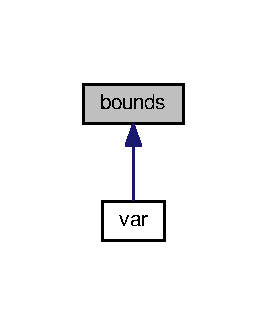
\includegraphics[width=128pt]{structbounds__inherit__graph}
\end{center}
\end{figure}
\subsection*{Public Member Functions}
\begin{DoxyCompactItemize}
\item 
\hyperlink{structbounds_a8441bf308868cb8a69004ba7390a2a36}{$\sim$bounds} ()
\end{DoxyCompactItemize}
\subsection*{Public Attributes}
\begin{DoxyCompactItemize}
\item 
int \hyperlink{structbounds_aa7cba1824fe84287bd4218054fa99975}{type}
\item 
double \hyperlink{structbounds_a972c937ccb85a76f76f653f7fc22054e}{lb}
\item 
double \hyperlink{structbounds_aad20828a963e0779a3cd3eb94ca1fecd}{ub}
\end{DoxyCompactItemize}


\subsection{Constructor \& Destructor Documentation}
\hypertarget{structbounds_a8441bf308868cb8a69004ba7390a2a36}{\index{bounds@{bounds}!$\sim$bounds@{$\sim$bounds}}
\index{$\sim$bounds@{$\sim$bounds}!bounds@{bounds}}
\subsubsection[{$\sim$bounds}]{\setlength{\rightskip}{0pt plus 5cm}bounds\-::$\sim$bounds (
\begin{DoxyParamCaption}
{}
\end{DoxyParamCaption}
)\hspace{0.3cm}{\ttfamily [inline]}}}\label{structbounds_a8441bf308868cb8a69004ba7390a2a36}


\subsection{Member Data Documentation}
\hypertarget{structbounds_a972c937ccb85a76f76f653f7fc22054e}{\index{bounds@{bounds}!lb@{lb}}
\index{lb@{lb}!bounds@{bounds}}
\subsubsection[{lb}]{\setlength{\rightskip}{0pt plus 5cm}double bounds\-::lb}}\label{structbounds_a972c937ccb85a76f76f653f7fc22054e}
\hypertarget{structbounds_aa7cba1824fe84287bd4218054fa99975}{\index{bounds@{bounds}!type@{type}}
\index{type@{type}!bounds@{bounds}}
\subsubsection[{type}]{\setlength{\rightskip}{0pt plus 5cm}int bounds\-::type}}\label{structbounds_aa7cba1824fe84287bd4218054fa99975}
\hypertarget{structbounds_aad20828a963e0779a3cd3eb94ca1fecd}{\index{bounds@{bounds}!ub@{ub}}
\index{ub@{ub}!bounds@{bounds}}
\subsubsection[{ub}]{\setlength{\rightskip}{0pt plus 5cm}double bounds\-::ub}}\label{structbounds_aad20828a963e0779a3cd3eb94ca1fecd}


The documentation for this struct was generated from the following file\-:\begin{DoxyCompactItemize}
\item 
\hyperlink{_b_p___data_8hpp}{B\-P\-\_\-\-Data.\-hpp}\end{DoxyCompactItemize}

\hypertarget{class_b_p___input}{\section{B\-P\-\_\-\-Input Class Reference}
\label{class_b_p___input}\index{B\-P\-\_\-\-Input@{B\-P\-\_\-\-Input}}
}


{\ttfamily \#include $<$B\-P\-\_\-\-Data.\-hpp$>$}

\subsection*{Public Member Functions}
\begin{DoxyCompactItemize}
\item 
\hyperlink{class_b_p___input_af11c6d9710bee39d23a4abba20cb630f}{B\-P\-\_\-\-Input} (string file\-\_\-name)
\item 
\hyperlink{structbounds}{bounds} \hyperlink{class_b_p___input_af4d2583195fd4629455d74923ca499fe}{get\-Bterms} (const int i) const 
\item 
const vector$<$ \hyperlink{structelem}{elem} $>$ \& \hyperlink{class_b_p___input_adef364bb6eca83f1deab8c450bd64352}{get\-Matcoeff} (const int i) const 
\item 
const vector$<$ \hyperlink{structelem}{elem} $>$ \& \hyperlink{class_b_p___input_ac9ac75a8da307b1a4f4c5d19fa8fd456}{get\-Matcoeff2} (const int j) const 
\item 
unsigned \hyperlink{class_b_p___input_a945d4a08729b49412a9a94e7df780ab0}{get\-Ncons} () const 
\item 
unsigned \hyperlink{class_b_p___input_a6d6f9c288b6349bbbbbda2bacf367985}{get\-Nvars} () const 
\item 
\hyperlink{structvar}{var} \hyperlink{class_b_p___input_a0e7dbca96bff6f3e143485584deec724}{get\-Var} (const int j) const 
\item 
vector$<$ \hyperlink{structvar}{var} $>$ \hyperlink{class_b_p___input_a05c2c750e02a0a2fd9de1ae0aa7a14c0}{get\-Vars} () const 
\item 
int \hyperlink{class_b_p___input_a82efaa6879d5c37d50fe82d71628c03f}{get\-Direction} () const 
\item 
unsigned \hyperlink{class_b_p___input_ac760da883346d05855da604a0f418e68}{get\-Scale} () const 
\item 
void \hyperlink{class_b_p___input_a6858da37c5b259b8b7d5c59fbd65acb3}{set\-Digits} (double number)
\item 
\hyperlink{class_b_p___input_a3341717cf5481b2369b600901ab5450d}{$\sim$\-B\-P\-\_\-\-Input} ()
\end{DoxyCompactItemize}
\subsection*{Protected Attributes}
\begin{DoxyCompactItemize}
\item 
int \hyperlink{class_b_p___input_a5852fa6f08df71a7e6f7da18d29d00fb}{nvars}
\item 
int \hyperlink{class_b_p___input_aa4e9401b70ce5a85684c826dc91f0e22}{ncons}
\item 
int \hyperlink{class_b_p___input_a9248e80975fe67559644a53be0fdaced}{nbinvars}
\item 
int \hyperlink{class_b_p___input_a26d89d84381b238db05b8c89d7b948ce}{nintvars}
\item 
int \hyperlink{class_b_p___input_a815e964e6687ba9572ff5eded8428ab7}{direction}
\item 
unsigned \hyperlink{class_b_p___input_acee50c002d8261ef1b0fdd05af99c659}{scale}
\item 
vector$<$ vector$<$ \hyperlink{structelem}{elem} $>$ $>$ \hyperlink{class_b_p___input_ab55ff15bb47a828b7a3c83c32e1c18c3}{matcoeff}
\item 
vector$<$ vector$<$ \hyperlink{structelem}{elem} $>$ $>$ \hyperlink{class_b_p___input_a213441fb4dcffbe23c104142b4169d42}{matcoeff2}
\item 
vector$<$ \hyperlink{structbounds}{bounds} $>$ \hyperlink{class_b_p___input_a964eaa6ceec4d2edf5ab2e70338077a5}{bterms}
\item 
vector$<$ \hyperlink{structvar}{var} $>$ \hyperlink{class_b_p___input_a57b4dee2857fb8155af4521fca27fb89}{vars}
\end{DoxyCompactItemize}
\subsection*{Friends}
\begin{DoxyCompactItemize}
\item 
ostream \& \hyperlink{class_b_p___input_a5df5090f211b1f324a0318de57eed9f4}{operator$<$$<$} (ostream \&os, const \hyperlink{class_b_p___input}{B\-P\-\_\-\-Input} \&bs)
\end{DoxyCompactItemize}


\subsection{Constructor \& Destructor Documentation}
\hypertarget{class_b_p___input_af11c6d9710bee39d23a4abba20cb630f}{\index{B\-P\-\_\-\-Input@{B\-P\-\_\-\-Input}!B\-P\-\_\-\-Input@{B\-P\-\_\-\-Input}}
\index{B\-P\-\_\-\-Input@{B\-P\-\_\-\-Input}!BP_Input@{B\-P\-\_\-\-Input}}
\subsubsection[{B\-P\-\_\-\-Input}]{\setlength{\rightskip}{0pt plus 5cm}B\-P\-\_\-\-Input\-::\-B\-P\-\_\-\-Input (
\begin{DoxyParamCaption}
\item[{string}]{file\-\_\-name}
\end{DoxyParamCaption}
)}}\label{class_b_p___input_af11c6d9710bee39d23a4abba20cb630f}
\hypertarget{class_b_p___input_a3341717cf5481b2369b600901ab5450d}{\index{B\-P\-\_\-\-Input@{B\-P\-\_\-\-Input}!$\sim$\-B\-P\-\_\-\-Input@{$\sim$\-B\-P\-\_\-\-Input}}
\index{$\sim$\-B\-P\-\_\-\-Input@{$\sim$\-B\-P\-\_\-\-Input}!BP_Input@{B\-P\-\_\-\-Input}}
\subsubsection[{$\sim$\-B\-P\-\_\-\-Input}]{\setlength{\rightskip}{0pt plus 5cm}B\-P\-\_\-\-Input\-::$\sim$\-B\-P\-\_\-\-Input (
\begin{DoxyParamCaption}
{}
\end{DoxyParamCaption}
)\hspace{0.3cm}{\ttfamily [inline]}}}\label{class_b_p___input_a3341717cf5481b2369b600901ab5450d}


\subsection{Member Function Documentation}
\hypertarget{class_b_p___input_af4d2583195fd4629455d74923ca499fe}{\index{B\-P\-\_\-\-Input@{B\-P\-\_\-\-Input}!get\-Bterms@{get\-Bterms}}
\index{get\-Bterms@{get\-Bterms}!BP_Input@{B\-P\-\_\-\-Input}}
\subsubsection[{get\-Bterms}]{\setlength{\rightskip}{0pt plus 5cm}{\bf bounds} B\-P\-\_\-\-Input\-::get\-Bterms (
\begin{DoxyParamCaption}
\item[{const int}]{i}
\end{DoxyParamCaption}
) const\hspace{0.3cm}{\ttfamily [inline]}}}\label{class_b_p___input_af4d2583195fd4629455d74923ca499fe}
\hypertarget{class_b_p___input_a82efaa6879d5c37d50fe82d71628c03f}{\index{B\-P\-\_\-\-Input@{B\-P\-\_\-\-Input}!get\-Direction@{get\-Direction}}
\index{get\-Direction@{get\-Direction}!BP_Input@{B\-P\-\_\-\-Input}}
\subsubsection[{get\-Direction}]{\setlength{\rightskip}{0pt plus 5cm}int B\-P\-\_\-\-Input\-::get\-Direction (
\begin{DoxyParamCaption}
{}
\end{DoxyParamCaption}
) const\hspace{0.3cm}{\ttfamily [inline]}}}\label{class_b_p___input_a82efaa6879d5c37d50fe82d71628c03f}
\hypertarget{class_b_p___input_adef364bb6eca83f1deab8c450bd64352}{\index{B\-P\-\_\-\-Input@{B\-P\-\_\-\-Input}!get\-Matcoeff@{get\-Matcoeff}}
\index{get\-Matcoeff@{get\-Matcoeff}!BP_Input@{B\-P\-\_\-\-Input}}
\subsubsection[{get\-Matcoeff}]{\setlength{\rightskip}{0pt plus 5cm}const vector$<${\bf elem}$>$\& B\-P\-\_\-\-Input\-::get\-Matcoeff (
\begin{DoxyParamCaption}
\item[{const int}]{i}
\end{DoxyParamCaption}
) const\hspace{0.3cm}{\ttfamily [inline]}}}\label{class_b_p___input_adef364bb6eca83f1deab8c450bd64352}
\hypertarget{class_b_p___input_ac9ac75a8da307b1a4f4c5d19fa8fd456}{\index{B\-P\-\_\-\-Input@{B\-P\-\_\-\-Input}!get\-Matcoeff2@{get\-Matcoeff2}}
\index{get\-Matcoeff2@{get\-Matcoeff2}!BP_Input@{B\-P\-\_\-\-Input}}
\subsubsection[{get\-Matcoeff2}]{\setlength{\rightskip}{0pt plus 5cm}const vector$<${\bf elem}$>$\& B\-P\-\_\-\-Input\-::get\-Matcoeff2 (
\begin{DoxyParamCaption}
\item[{const int}]{j}
\end{DoxyParamCaption}
) const\hspace{0.3cm}{\ttfamily [inline]}}}\label{class_b_p___input_ac9ac75a8da307b1a4f4c5d19fa8fd456}
\hypertarget{class_b_p___input_a945d4a08729b49412a9a94e7df780ab0}{\index{B\-P\-\_\-\-Input@{B\-P\-\_\-\-Input}!get\-Ncons@{get\-Ncons}}
\index{get\-Ncons@{get\-Ncons}!BP_Input@{B\-P\-\_\-\-Input}}
\subsubsection[{get\-Ncons}]{\setlength{\rightskip}{0pt plus 5cm}unsigned B\-P\-\_\-\-Input\-::get\-Ncons (
\begin{DoxyParamCaption}
{}
\end{DoxyParamCaption}
) const\hspace{0.3cm}{\ttfamily [inline]}}}\label{class_b_p___input_a945d4a08729b49412a9a94e7df780ab0}
\hypertarget{class_b_p___input_a6d6f9c288b6349bbbbbda2bacf367985}{\index{B\-P\-\_\-\-Input@{B\-P\-\_\-\-Input}!get\-Nvars@{get\-Nvars}}
\index{get\-Nvars@{get\-Nvars}!BP_Input@{B\-P\-\_\-\-Input}}
\subsubsection[{get\-Nvars}]{\setlength{\rightskip}{0pt plus 5cm}unsigned B\-P\-\_\-\-Input\-::get\-Nvars (
\begin{DoxyParamCaption}
{}
\end{DoxyParamCaption}
) const\hspace{0.3cm}{\ttfamily [inline]}}}\label{class_b_p___input_a6d6f9c288b6349bbbbbda2bacf367985}
\hypertarget{class_b_p___input_ac760da883346d05855da604a0f418e68}{\index{B\-P\-\_\-\-Input@{B\-P\-\_\-\-Input}!get\-Scale@{get\-Scale}}
\index{get\-Scale@{get\-Scale}!BP_Input@{B\-P\-\_\-\-Input}}
\subsubsection[{get\-Scale}]{\setlength{\rightskip}{0pt plus 5cm}unsigned B\-P\-\_\-\-Input\-::get\-Scale (
\begin{DoxyParamCaption}
{}
\end{DoxyParamCaption}
) const\hspace{0.3cm}{\ttfamily [inline]}}}\label{class_b_p___input_ac760da883346d05855da604a0f418e68}
\hypertarget{class_b_p___input_a0e7dbca96bff6f3e143485584deec724}{\index{B\-P\-\_\-\-Input@{B\-P\-\_\-\-Input}!get\-Var@{get\-Var}}
\index{get\-Var@{get\-Var}!BP_Input@{B\-P\-\_\-\-Input}}
\subsubsection[{get\-Var}]{\setlength{\rightskip}{0pt plus 5cm}{\bf var} B\-P\-\_\-\-Input\-::get\-Var (
\begin{DoxyParamCaption}
\item[{const int}]{j}
\end{DoxyParamCaption}
) const\hspace{0.3cm}{\ttfamily [inline]}}}\label{class_b_p___input_a0e7dbca96bff6f3e143485584deec724}
\hypertarget{class_b_p___input_a05c2c750e02a0a2fd9de1ae0aa7a14c0}{\index{B\-P\-\_\-\-Input@{B\-P\-\_\-\-Input}!get\-Vars@{get\-Vars}}
\index{get\-Vars@{get\-Vars}!BP_Input@{B\-P\-\_\-\-Input}}
\subsubsection[{get\-Vars}]{\setlength{\rightskip}{0pt plus 5cm}vector$<${\bf var}$>$ B\-P\-\_\-\-Input\-::get\-Vars (
\begin{DoxyParamCaption}
{}
\end{DoxyParamCaption}
) const\hspace{0.3cm}{\ttfamily [inline]}}}\label{class_b_p___input_a05c2c750e02a0a2fd9de1ae0aa7a14c0}
\hypertarget{class_b_p___input_a6858da37c5b259b8b7d5c59fbd65acb3}{\index{B\-P\-\_\-\-Input@{B\-P\-\_\-\-Input}!set\-Digits@{set\-Digits}}
\index{set\-Digits@{set\-Digits}!BP_Input@{B\-P\-\_\-\-Input}}
\subsubsection[{set\-Digits}]{\setlength{\rightskip}{0pt plus 5cm}void B\-P\-\_\-\-Input\-::set\-Digits (
\begin{DoxyParamCaption}
\item[{double}]{number}
\end{DoxyParamCaption}
)}}\label{class_b_p___input_a6858da37c5b259b8b7d5c59fbd65acb3}


\subsection{Friends And Related Function Documentation}
\hypertarget{class_b_p___input_a5df5090f211b1f324a0318de57eed9f4}{\index{B\-P\-\_\-\-Input@{B\-P\-\_\-\-Input}!operator$<$$<$@{operator$<$$<$}}
\index{operator$<$$<$@{operator$<$$<$}!BP_Input@{B\-P\-\_\-\-Input}}
\subsubsection[{operator$<$$<$}]{\setlength{\rightskip}{0pt plus 5cm}ostream\& operator$<$$<$ (
\begin{DoxyParamCaption}
\item[{ostream \&}]{os, }
\item[{const {\bf B\-P\-\_\-\-Input} \&}]{bs}
\end{DoxyParamCaption}
)\hspace{0.3cm}{\ttfamily [friend]}}}\label{class_b_p___input_a5df5090f211b1f324a0318de57eed9f4}


\subsection{Member Data Documentation}
\hypertarget{class_b_p___input_a964eaa6ceec4d2edf5ab2e70338077a5}{\index{B\-P\-\_\-\-Input@{B\-P\-\_\-\-Input}!bterms@{bterms}}
\index{bterms@{bterms}!BP_Input@{B\-P\-\_\-\-Input}}
\subsubsection[{bterms}]{\setlength{\rightskip}{0pt plus 5cm}vector$<${\bf bounds}$>$ B\-P\-\_\-\-Input\-::bterms\hspace{0.3cm}{\ttfamily [protected]}}}\label{class_b_p___input_a964eaa6ceec4d2edf5ab2e70338077a5}
\hypertarget{class_b_p___input_a815e964e6687ba9572ff5eded8428ab7}{\index{B\-P\-\_\-\-Input@{B\-P\-\_\-\-Input}!direction@{direction}}
\index{direction@{direction}!BP_Input@{B\-P\-\_\-\-Input}}
\subsubsection[{direction}]{\setlength{\rightskip}{0pt plus 5cm}int B\-P\-\_\-\-Input\-::direction\hspace{0.3cm}{\ttfamily [protected]}}}\label{class_b_p___input_a815e964e6687ba9572ff5eded8428ab7}
\hypertarget{class_b_p___input_ab55ff15bb47a828b7a3c83c32e1c18c3}{\index{B\-P\-\_\-\-Input@{B\-P\-\_\-\-Input}!matcoeff@{matcoeff}}
\index{matcoeff@{matcoeff}!BP_Input@{B\-P\-\_\-\-Input}}
\subsubsection[{matcoeff}]{\setlength{\rightskip}{0pt plus 5cm}vector$<$vector$<${\bf elem}$>$ $>$ B\-P\-\_\-\-Input\-::matcoeff\hspace{0.3cm}{\ttfamily [protected]}}}\label{class_b_p___input_ab55ff15bb47a828b7a3c83c32e1c18c3}
\hypertarget{class_b_p___input_a213441fb4dcffbe23c104142b4169d42}{\index{B\-P\-\_\-\-Input@{B\-P\-\_\-\-Input}!matcoeff2@{matcoeff2}}
\index{matcoeff2@{matcoeff2}!BP_Input@{B\-P\-\_\-\-Input}}
\subsubsection[{matcoeff2}]{\setlength{\rightskip}{0pt plus 5cm}vector$<$vector$<${\bf elem}$>$ $>$ B\-P\-\_\-\-Input\-::matcoeff2\hspace{0.3cm}{\ttfamily [protected]}}}\label{class_b_p___input_a213441fb4dcffbe23c104142b4169d42}
\hypertarget{class_b_p___input_a9248e80975fe67559644a53be0fdaced}{\index{B\-P\-\_\-\-Input@{B\-P\-\_\-\-Input}!nbinvars@{nbinvars}}
\index{nbinvars@{nbinvars}!BP_Input@{B\-P\-\_\-\-Input}}
\subsubsection[{nbinvars}]{\setlength{\rightskip}{0pt plus 5cm}int B\-P\-\_\-\-Input\-::nbinvars\hspace{0.3cm}{\ttfamily [protected]}}}\label{class_b_p___input_a9248e80975fe67559644a53be0fdaced}
\hypertarget{class_b_p___input_aa4e9401b70ce5a85684c826dc91f0e22}{\index{B\-P\-\_\-\-Input@{B\-P\-\_\-\-Input}!ncons@{ncons}}
\index{ncons@{ncons}!BP_Input@{B\-P\-\_\-\-Input}}
\subsubsection[{ncons}]{\setlength{\rightskip}{0pt plus 5cm}int B\-P\-\_\-\-Input\-::ncons\hspace{0.3cm}{\ttfamily [protected]}}}\label{class_b_p___input_aa4e9401b70ce5a85684c826dc91f0e22}
\hypertarget{class_b_p___input_a26d89d84381b238db05b8c89d7b948ce}{\index{B\-P\-\_\-\-Input@{B\-P\-\_\-\-Input}!nintvars@{nintvars}}
\index{nintvars@{nintvars}!BP_Input@{B\-P\-\_\-\-Input}}
\subsubsection[{nintvars}]{\setlength{\rightskip}{0pt plus 5cm}int B\-P\-\_\-\-Input\-::nintvars\hspace{0.3cm}{\ttfamily [protected]}}}\label{class_b_p___input_a26d89d84381b238db05b8c89d7b948ce}
\hypertarget{class_b_p___input_a5852fa6f08df71a7e6f7da18d29d00fb}{\index{B\-P\-\_\-\-Input@{B\-P\-\_\-\-Input}!nvars@{nvars}}
\index{nvars@{nvars}!BP_Input@{B\-P\-\_\-\-Input}}
\subsubsection[{nvars}]{\setlength{\rightskip}{0pt plus 5cm}int B\-P\-\_\-\-Input\-::nvars\hspace{0.3cm}{\ttfamily [protected]}}}\label{class_b_p___input_a5852fa6f08df71a7e6f7da18d29d00fb}
\hypertarget{class_b_p___input_acee50c002d8261ef1b0fdd05af99c659}{\index{B\-P\-\_\-\-Input@{B\-P\-\_\-\-Input}!scale@{scale}}
\index{scale@{scale}!BP_Input@{B\-P\-\_\-\-Input}}
\subsubsection[{scale}]{\setlength{\rightskip}{0pt plus 5cm}unsigned B\-P\-\_\-\-Input\-::scale\hspace{0.3cm}{\ttfamily [protected]}}}\label{class_b_p___input_acee50c002d8261ef1b0fdd05af99c659}
\hypertarget{class_b_p___input_a57b4dee2857fb8155af4521fca27fb89}{\index{B\-P\-\_\-\-Input@{B\-P\-\_\-\-Input}!vars@{vars}}
\index{vars@{vars}!BP_Input@{B\-P\-\_\-\-Input}}
\subsubsection[{vars}]{\setlength{\rightskip}{0pt plus 5cm}vector$<${\bf var}$>$ B\-P\-\_\-\-Input\-::vars\hspace{0.3cm}{\ttfamily [protected]}}}\label{class_b_p___input_a57b4dee2857fb8155af4521fca27fb89}


The documentation for this class was generated from the following files\-:\begin{DoxyCompactItemize}
\item 
\hyperlink{_b_p___data_8hpp}{B\-P\-\_\-\-Data.\-hpp}\item 
\hyperlink{_b_p___data_8cpp}{B\-P\-\_\-\-Data.\-cpp}\end{DoxyCompactItemize}

\hypertarget{class_b_p___output}{\section{B\-P\-\_\-\-Output Class Reference}
\label{class_b_p___output}\index{B\-P\-\_\-\-Output@{B\-P\-\_\-\-Output}}
}


{\ttfamily \#include $<$B\-P\-\_\-\-Data.\-hpp$>$}



Collaboration diagram for B\-P\-\_\-\-Output\-:\nopagebreak
\begin{figure}[H]
\begin{center}
\leavevmode
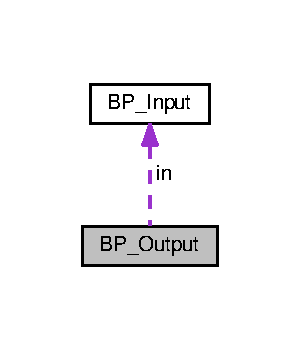
\includegraphics[width=144pt]{class_b_p___output__coll__graph}
\end{center}
\end{figure}
\subsection*{Public Member Functions}
\begin{DoxyCompactItemize}
\item 
\hyperlink{class_b_p___output_a1b18890b45b21a2986a489a8699891e9}{B\-P\-\_\-\-Output} (const \hyperlink{class_b_p___input}{B\-P\-\_\-\-Input} \&i)
\item 
\hyperlink{class_b_p___output}{B\-P\-\_\-\-Output} \& \hyperlink{class_b_p___output_a5885aba4ce5e63e08a7ccac9d2a409ed}{operator=} (const \hyperlink{class_b_p___output}{B\-P\-\_\-\-Output} \&out)
\item 
int \hyperlink{class_b_p___output_ab04e487bb643ea365287b5b1e86b6197}{assignment} (int \hyperlink{structvar}{var}) const 
\item 
void \hyperlink{class_b_p___output_afffa35963a12e9175a680eb14949e642}{assign} (int \hyperlink{structvar}{var}, bool b)
\end{DoxyCompactItemize}
\subsection*{Protected Attributes}
\begin{DoxyCompactItemize}
\item 
const \hyperlink{class_b_p___input}{B\-P\-\_\-\-Input} \& \hyperlink{class_b_p___output_a84649c3f9e29b7fdf080419ff590c096}{in}
\item 
vector$<$ bool $>$ \hyperlink{class_b_p___output_a581b177c0383ee72b0395595641fb82b}{var\-Assignment}
\end{DoxyCompactItemize}
\subsection*{Friends}
\begin{DoxyCompactItemize}
\item 
ostream \& \hyperlink{class_b_p___output_a1d1741e17f725be51640a6d881d768fa}{operator$<$$<$} (ostream \&os, const \hyperlink{class_b_p___output}{B\-P\-\_\-\-Output} \&out)
\item 
istream \& \hyperlink{class_b_p___output_a401e305330b684d15b38d6a6a0bfb25f}{operator$>$$>$} (istream \&is, \hyperlink{class_b_p___output}{B\-P\-\_\-\-Output} \&out)
\end{DoxyCompactItemize}


\subsection{Constructor \& Destructor Documentation}
\hypertarget{class_b_p___output_a1b18890b45b21a2986a489a8699891e9}{\index{B\-P\-\_\-\-Output@{B\-P\-\_\-\-Output}!B\-P\-\_\-\-Output@{B\-P\-\_\-\-Output}}
\index{B\-P\-\_\-\-Output@{B\-P\-\_\-\-Output}!BP_Output@{B\-P\-\_\-\-Output}}
\subsubsection[{B\-P\-\_\-\-Output}]{\setlength{\rightskip}{0pt plus 5cm}B\-P\-\_\-\-Output\-::\-B\-P\-\_\-\-Output (
\begin{DoxyParamCaption}
\item[{const {\bf B\-P\-\_\-\-Input} \&}]{i}
\end{DoxyParamCaption}
)}}\label{class_b_p___output_a1b18890b45b21a2986a489a8699891e9}


\subsection{Member Function Documentation}
\hypertarget{class_b_p___output_afffa35963a12e9175a680eb14949e642}{\index{B\-P\-\_\-\-Output@{B\-P\-\_\-\-Output}!assign@{assign}}
\index{assign@{assign}!BP_Output@{B\-P\-\_\-\-Output}}
\subsubsection[{assign}]{\setlength{\rightskip}{0pt plus 5cm}void B\-P\-\_\-\-Output\-::assign (
\begin{DoxyParamCaption}
\item[{int}]{var, }
\item[{bool}]{b}
\end{DoxyParamCaption}
)}}\label{class_b_p___output_afffa35963a12e9175a680eb14949e642}
\hypertarget{class_b_p___output_ab04e487bb643ea365287b5b1e86b6197}{\index{B\-P\-\_\-\-Output@{B\-P\-\_\-\-Output}!assignment@{assignment}}
\index{assignment@{assignment}!BP_Output@{B\-P\-\_\-\-Output}}
\subsubsection[{assignment}]{\setlength{\rightskip}{0pt plus 5cm}int B\-P\-\_\-\-Output\-::assignment (
\begin{DoxyParamCaption}
\item[{int}]{var}
\end{DoxyParamCaption}
) const\hspace{0.3cm}{\ttfamily [inline]}}}\label{class_b_p___output_ab04e487bb643ea365287b5b1e86b6197}
\hypertarget{class_b_p___output_a5885aba4ce5e63e08a7ccac9d2a409ed}{\index{B\-P\-\_\-\-Output@{B\-P\-\_\-\-Output}!operator=@{operator=}}
\index{operator=@{operator=}!BP_Output@{B\-P\-\_\-\-Output}}
\subsubsection[{operator=}]{\setlength{\rightskip}{0pt plus 5cm}{\bf B\-P\-\_\-\-Output} \& B\-P\-\_\-\-Output\-::operator= (
\begin{DoxyParamCaption}
\item[{const {\bf B\-P\-\_\-\-Output} \&}]{out}
\end{DoxyParamCaption}
)}}\label{class_b_p___output_a5885aba4ce5e63e08a7ccac9d2a409ed}


\subsection{Friends And Related Function Documentation}
\hypertarget{class_b_p___output_a1d1741e17f725be51640a6d881d768fa}{\index{B\-P\-\_\-\-Output@{B\-P\-\_\-\-Output}!operator$<$$<$@{operator$<$$<$}}
\index{operator$<$$<$@{operator$<$$<$}!BP_Output@{B\-P\-\_\-\-Output}}
\subsubsection[{operator$<$$<$}]{\setlength{\rightskip}{0pt plus 5cm}ostream\& operator$<$$<$ (
\begin{DoxyParamCaption}
\item[{ostream \&}]{os, }
\item[{const {\bf B\-P\-\_\-\-Output} \&}]{out}
\end{DoxyParamCaption}
)\hspace{0.3cm}{\ttfamily [friend]}}}\label{class_b_p___output_a1d1741e17f725be51640a6d881d768fa}
\hypertarget{class_b_p___output_a401e305330b684d15b38d6a6a0bfb25f}{\index{B\-P\-\_\-\-Output@{B\-P\-\_\-\-Output}!operator$>$$>$@{operator$>$$>$}}
\index{operator$>$$>$@{operator$>$$>$}!BP_Output@{B\-P\-\_\-\-Output}}
\subsubsection[{operator$>$$>$}]{\setlength{\rightskip}{0pt plus 5cm}istream\& operator$>$$>$ (
\begin{DoxyParamCaption}
\item[{istream \&}]{is, }
\item[{{\bf B\-P\-\_\-\-Output} \&}]{out}
\end{DoxyParamCaption}
)\hspace{0.3cm}{\ttfamily [friend]}}}\label{class_b_p___output_a401e305330b684d15b38d6a6a0bfb25f}


\subsection{Member Data Documentation}
\hypertarget{class_b_p___output_a84649c3f9e29b7fdf080419ff590c096}{\index{B\-P\-\_\-\-Output@{B\-P\-\_\-\-Output}!in@{in}}
\index{in@{in}!BP_Output@{B\-P\-\_\-\-Output}}
\subsubsection[{in}]{\setlength{\rightskip}{0pt plus 5cm}const {\bf B\-P\-\_\-\-Input}\& B\-P\-\_\-\-Output\-::in\hspace{0.3cm}{\ttfamily [protected]}}}\label{class_b_p___output_a84649c3f9e29b7fdf080419ff590c096}
\hypertarget{class_b_p___output_a581b177c0383ee72b0395595641fb82b}{\index{B\-P\-\_\-\-Output@{B\-P\-\_\-\-Output}!var\-Assignment@{var\-Assignment}}
\index{var\-Assignment@{var\-Assignment}!BP_Output@{B\-P\-\_\-\-Output}}
\subsubsection[{var\-Assignment}]{\setlength{\rightskip}{0pt plus 5cm}vector$<$bool$>$ B\-P\-\_\-\-Output\-::var\-Assignment\hspace{0.3cm}{\ttfamily [protected]}}}\label{class_b_p___output_a581b177c0383ee72b0395595641fb82b}


The documentation for this class was generated from the following files\-:\begin{DoxyCompactItemize}
\item 
\hyperlink{_b_p___data_8hpp}{B\-P\-\_\-\-Data.\-hpp}\item 
\hyperlink{_b_p___data_8cpp}{B\-P\-\_\-\-Data.\-cpp}\end{DoxyCompactItemize}

\hypertarget{class_b_p_solver}{\section{B\-P\-Solver Class Reference}
\label{class_b_p_solver}\index{B\-P\-Solver@{B\-P\-Solver}}
}


{\ttfamily \#include $<$B\-P\-Solver.\-hpp$>$}



Inheritance diagram for B\-P\-Solver\-:\nopagebreak
\begin{figure}[H]
\begin{center}
\leavevmode
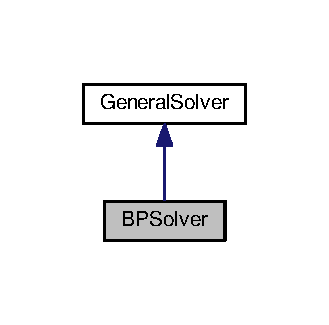
\includegraphics[width=158pt]{class_b_p_solver__inherit__graph}
\end{center}
\end{figure}


Collaboration diagram for B\-P\-Solver\-:\nopagebreak
\begin{figure}[H]
\begin{center}
\leavevmode
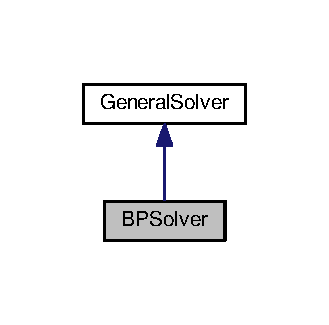
\includegraphics[width=158pt]{class_b_p_solver__coll__graph}
\end{center}
\end{figure}
\subsection*{Public Member Functions}
\begin{DoxyCompactItemize}
\item 
\hyperlink{class_b_p_solver_ade768d74f063c00a42b7e4a86f68ff01}{B\-P\-Solver} (\hyperlink{class_b_p___input}{B\-P\-\_\-\-Input} $\ast$in)
\item 
\hyperlink{class_b_p_solver_a22159c0b1f342264f8271b8f44d260ab}{$\sim$\-B\-P\-Solver} ()
\item 
void \hyperlink{class_b_p_solver_adeb9db9fda332fb71b99262973a48d3f}{print\-Current} ()
\begin{DoxyCompactList}\small\item\em Constructor for cloning s. \end{DoxyCompactList}\end{DoxyCompactItemize}


\subsection{Constructor \& Destructor Documentation}
\hypertarget{class_b_p_solver_ade768d74f063c00a42b7e4a86f68ff01}{\index{B\-P\-Solver@{B\-P\-Solver}!B\-P\-Solver@{B\-P\-Solver}}
\index{B\-P\-Solver@{B\-P\-Solver}!BPSolver@{B\-P\-Solver}}
\subsubsection[{B\-P\-Solver}]{\setlength{\rightskip}{0pt plus 5cm}B\-P\-Solver\-::\-B\-P\-Solver (
\begin{DoxyParamCaption}
\item[{{\bf B\-P\-\_\-\-Input} $\ast$}]{in}
\end{DoxyParamCaption}
)\hspace{0.3cm}{\ttfamily [inline]}}}\label{class_b_p_solver_ade768d74f063c00a42b7e4a86f68ff01}
\hypertarget{class_b_p_solver_a22159c0b1f342264f8271b8f44d260ab}{\index{B\-P\-Solver@{B\-P\-Solver}!$\sim$\-B\-P\-Solver@{$\sim$\-B\-P\-Solver}}
\index{$\sim$\-B\-P\-Solver@{$\sim$\-B\-P\-Solver}!BPSolver@{B\-P\-Solver}}
\subsubsection[{$\sim$\-B\-P\-Solver}]{\setlength{\rightskip}{0pt plus 5cm}B\-P\-Solver\-::$\sim$\-B\-P\-Solver (
\begin{DoxyParamCaption}
{}
\end{DoxyParamCaption}
)\hspace{0.3cm}{\ttfamily [inline]}}}\label{class_b_p_solver_a22159c0b1f342264f8271b8f44d260ab}


\subsection{Member Function Documentation}
\hypertarget{class_b_p_solver_adeb9db9fda332fb71b99262973a48d3f}{\index{B\-P\-Solver@{B\-P\-Solver}!print\-Current@{print\-Current}}
\index{print\-Current@{print\-Current}!BPSolver@{B\-P\-Solver}}
\subsubsection[{print\-Current}]{\setlength{\rightskip}{0pt plus 5cm}void B\-P\-Solver\-::print\-Current (
\begin{DoxyParamCaption}
{}
\end{DoxyParamCaption}
)\hspace{0.3cm}{\ttfamily [inline]}}}\label{class_b_p_solver_adeb9db9fda332fb71b99262973a48d3f}


Constructor for cloning s. 



The documentation for this class was generated from the following file\-:\begin{DoxyCompactItemize}
\item 
\hyperlink{_b_p_solver_8hpp}{B\-P\-Solver.\-hpp}\end{DoxyCompactItemize}

\hypertarget{class_clock}{\section{Clock Class Reference}
\label{class_clock}\index{Clock@{Clock}}
}


{\ttfamily \#include $<$Clock.\-hpp$>$}

\subsection*{Static Public Attributes}
\begin{DoxyCompactItemize}
\item 
static double \hyperlink{class_clock_a9ae2a018e36b6485f9be0117c381f523}{global\-Clock}
\end{DoxyCompactItemize}


\subsection{Member Data Documentation}
\hypertarget{class_clock_a9ae2a018e36b6485f9be0117c381f523}{\index{Clock@{Clock}!global\-Clock@{global\-Clock}}
\index{global\-Clock@{global\-Clock}!Clock@{Clock}}
\subsubsection[{global\-Clock}]{\setlength{\rightskip}{0pt plus 5cm}double Clock\-::global\-Clock\hspace{0.3cm}{\ttfamily [static]}}}\label{class_clock_a9ae2a018e36b6485f9be0117c381f523}


The documentation for this class was generated from the following files\-:\begin{DoxyCompactItemize}
\item 
\hyperlink{_clock_8hpp}{Clock.\-hpp}\item 
\hyperlink{_clock_8cpp}{Clock.\-cpp}\end{DoxyCompactItemize}

\hypertarget{class_constraint}{\section{Constraint Class Reference}
\label{class_constraint}\index{Constraint@{Constraint}}
}


{\ttfamily \#include $<$Constraint.\-hpp$>$}



Inheritance diagram for Constraint\-:\nopagebreak
\begin{figure}[H]
\begin{center}
\leavevmode
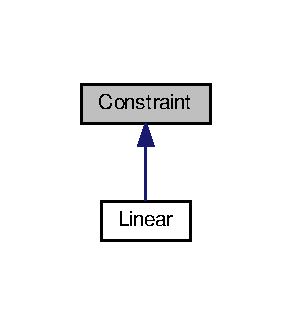
\includegraphics[width=140pt]{class_constraint__inherit__graph}
\end{center}
\end{figure}
\subsection*{Classes}
\begin{DoxyCompactItemize}
\item 
struct \hyperlink{struct_constraint_1_1_sort_greater}{Sort\-Greater}
\end{DoxyCompactItemize}
\subsection*{Public Member Functions}
\begin{DoxyCompactItemize}
\item 
\hyperlink{class_constraint_ac066210c674e540f0d2570f53d6eff7b}{Constraint} ()
\item 
\hyperlink{class_constraint_ae827fc88061ee544aca1cbe95a2c8389}{$\sim$\-Constraint} ()
\item 
void \hyperlink{class_constraint_a8feacaf03b5c6eae9058a9e20c99a829}{set\-Number\-Of\-Integer\-Variables} (int number)
\item 
int \& \hyperlink{class_constraint_a9638dcea0347e70974e9626d40ae651d}{get\-Number\-Of\-Integer\-Variables} ()
\item 
int \hyperlink{class_constraint_ac4dceb32e2f1b32b21503fb84a08026b}{get\-Type} ()
\item 
int \hyperlink{class_constraint_a357eac2af547bcc97ee202ea1b31589f}{get\-Delta\-Violation} ()
\item 
int \hyperlink{class_constraint_a77e02f7d1c968c170b20c44267be4d38}{get\-Delta\-Violation\-Degree} ()
\item 
int \hyperlink{class_constraint_a24d51a877159072275bd0b3eff9c3c86}{get\-Violation} ()
\item 
bool \hyperlink{class_constraint_aeeb7a31a623b2d875ca95c6cf9b5285f}{is\-Oneway} ()
\item 
void \hyperlink{class_constraint_a3d9519a131e3c36db21c589b8853a951}{is\-Oneway} (bool set)
\item 
std\-::unordered\-\_\-map$<$ int, \\*
\hyperlink{_constants_8hpp_a08c47c54ab9fb1545c341ec853cc2278}{coef\-Type} $>$ \& \hyperlink{class_constraint_a0b21be8f860e6daf62f465d9d7a090d8}{get\-Coefficients} ()
\item 
std\-::vector$<$ \hyperlink{class_integer_variable}{Integer\-Variable} $\ast$ $>$ \& \hyperlink{class_constraint_a699d1978b4903587950c9d7a0038bf37}{get\-Variables} ()
\item 
int \hyperlink{class_constraint_a4f98d1e3e4a24652dcd0c13f6b217cc8}{get\-Violation\-Degree} ()
\item 
int \hyperlink{class_constraint_a7db789c2e9f909d8e9ea8770a2b36b4d}{get\-Argument} (int i)
\item 
void \hyperlink{class_constraint_a92aa3050acb0fe8fca68bb0a00c472ec}{set\-Invariant} (std\-::shared\-\_\-ptr$<$ \hyperlink{class_invariant}{Invariant} $>$ invar)
\item 
std\-::shared\-\_\-ptr$<$ \hyperlink{class_invariant}{Invariant} $>$ \& \hyperlink{class_constraint_a4c202c55933908fb4e1caddf1a1711ec}{get\-Invariant} ()
\item 
unsigned \hyperlink{class_constraint_a972040ad73c82e1421c7a6ba160d1cfe}{get\-Scope\-Size} ()
\item 
bool \hyperlink{class_constraint_adc21199710e3a551b31122a8d9995c46}{operator$<$} (\hyperlink{class_constraint}{Constraint} \&cons) const 
\item 
bool \hyperlink{class_constraint_aabd1407d46c3907df989077e0a86d22b}{operator$>$} (\hyperlink{class_constraint}{Constraint} \&cons) const 
\item 
virtual int \hyperlink{class_constraint_a838ed3f4029d443c3193524be0c8f977}{set\-Delta\-Violation} ()
\item 
virtual int \hyperlink{class_constraint_aaa22c193fec13cbdc29875a1a90f65d6}{set\-Delta\-Violation\-Degree} ()
\item 
virtual int \hyperlink{class_constraint_a3dbfd62667a4d7c06fdfbd0b38608fca}{update\-Violation} ()
\item 
virtual int \hyperlink{class_constraint_a389d341b518e22981d7e8e4b8a16f739}{update\-Violation\-Degree} ()
\item 
virtual bool \hyperlink{class_constraint_affe33a000e4eedc012ae184617534225}{test\-Cons} ()
\item 
virtual bool \hyperlink{class_constraint_a564d47f24c7cdccf1c5a7b3fd91c0743}{test\-Obj} ()
\end{DoxyCompactItemize}
\subsection*{Protected Attributes}
\begin{DoxyCompactItemize}
\item 
int \hyperlink{class_constraint_ab80bb8ec253665f6572a94877579cdfb}{Violation} = 0
\item 
int \hyperlink{class_constraint_a673b620b0be43337a301c407afc15133}{Violation\-Degree} = 0
\item 
int \hyperlink{class_constraint_a8bddcdcac31ae446e91fd57a78841c75}{Delta\-Violation} = 0
\item 
int \hyperlink{class_constraint_a62ef0cdd114d9f44dbf4d07f9aa254f5}{Delta\-Violation\-Degree} = 0
\item 
int \hyperlink{class_constraint_a72868dc8e9187cc8eb8b43560890b895}{priority}
\item 
int \hyperlink{class_constraint_a377cd0c46beac0ad81d131b92824b626}{type}
\item 
bool \hyperlink{class_constraint_a9cc8e2f30e52abe6eb19311269f628ce}{oneway} = false
\item 
int \hyperlink{class_constraint_a010acf737425b29cb7a8f9263ecb02eb}{number\-Of\-Integer\-Variables} = 0
\item 
unsigned \hyperlink{class_constraint_afe1a5dbe5eb0c511d437d17c70960416}{scope\-Size}
\item 
std\-::vector$<$ int $>$ \hyperlink{class_constraint_a070f51ff894d874d90f550bbec989fe7}{arguments}
\item 
std\-::vector$<$ \hyperlink{class_integer_variable}{Integer\-Variable} $\ast$ $>$ \hyperlink{class_constraint_abd73767b8640c514f582a9316a1ce792}{variables}
\item 
std\-::unordered\-\_\-map$<$ int, \hyperlink{_constants_8hpp_a08c47c54ab9fb1545c341ec853cc2278}{coef\-Type} $>$ \hyperlink{class_constraint_a976da5d8a1e74efb119f47094b721df9}{coefficients}
\item 
std\-::shared\-\_\-ptr$<$ \hyperlink{class_invariant}{Invariant} $>$ \hyperlink{class_constraint_ad1aa16aebdbfff66d761850f0e70e5c8}{invariant}
\end{DoxyCompactItemize}


\subsection{Constructor \& Destructor Documentation}
\hypertarget{class_constraint_ac066210c674e540f0d2570f53d6eff7b}{\index{Constraint@{Constraint}!Constraint@{Constraint}}
\index{Constraint@{Constraint}!Constraint@{Constraint}}
\subsubsection[{Constraint}]{\setlength{\rightskip}{0pt plus 5cm}Constraint\-::\-Constraint (
\begin{DoxyParamCaption}
{}
\end{DoxyParamCaption}
)\hspace{0.3cm}{\ttfamily [inline]}}}\label{class_constraint_ac066210c674e540f0d2570f53d6eff7b}
\hypertarget{class_constraint_ae827fc88061ee544aca1cbe95a2c8389}{\index{Constraint@{Constraint}!$\sim$\-Constraint@{$\sim$\-Constraint}}
\index{$\sim$\-Constraint@{$\sim$\-Constraint}!Constraint@{Constraint}}
\subsubsection[{$\sim$\-Constraint}]{\setlength{\rightskip}{0pt plus 5cm}Constraint\-::$\sim$\-Constraint (
\begin{DoxyParamCaption}
{}
\end{DoxyParamCaption}
)\hspace{0.3cm}{\ttfamily [inline]}}}\label{class_constraint_ae827fc88061ee544aca1cbe95a2c8389}


\subsection{Member Function Documentation}
\hypertarget{class_constraint_a7db789c2e9f909d8e9ea8770a2b36b4d}{\index{Constraint@{Constraint}!get\-Argument@{get\-Argument}}
\index{get\-Argument@{get\-Argument}!Constraint@{Constraint}}
\subsubsection[{get\-Argument}]{\setlength{\rightskip}{0pt plus 5cm}int Constraint\-::get\-Argument (
\begin{DoxyParamCaption}
\item[{int}]{i}
\end{DoxyParamCaption}
)\hspace{0.3cm}{\ttfamily [inline]}}}\label{class_constraint_a7db789c2e9f909d8e9ea8770a2b36b4d}
\hypertarget{class_constraint_a0b21be8f860e6daf62f465d9d7a090d8}{\index{Constraint@{Constraint}!get\-Coefficients@{get\-Coefficients}}
\index{get\-Coefficients@{get\-Coefficients}!Constraint@{Constraint}}
\subsubsection[{get\-Coefficients}]{\setlength{\rightskip}{0pt plus 5cm}std\-::unordered\-\_\-map$<$int, {\bf coef\-Type}$>$\& Constraint\-::get\-Coefficients (
\begin{DoxyParamCaption}
{}
\end{DoxyParamCaption}
)\hspace{0.3cm}{\ttfamily [inline]}}}\label{class_constraint_a0b21be8f860e6daf62f465d9d7a090d8}
\hypertarget{class_constraint_a357eac2af547bcc97ee202ea1b31589f}{\index{Constraint@{Constraint}!get\-Delta\-Violation@{get\-Delta\-Violation}}
\index{get\-Delta\-Violation@{get\-Delta\-Violation}!Constraint@{Constraint}}
\subsubsection[{get\-Delta\-Violation}]{\setlength{\rightskip}{0pt plus 5cm}int Constraint\-::get\-Delta\-Violation (
\begin{DoxyParamCaption}
{}
\end{DoxyParamCaption}
)\hspace{0.3cm}{\ttfamily [inline]}}}\label{class_constraint_a357eac2af547bcc97ee202ea1b31589f}
\hypertarget{class_constraint_a77e02f7d1c968c170b20c44267be4d38}{\index{Constraint@{Constraint}!get\-Delta\-Violation\-Degree@{get\-Delta\-Violation\-Degree}}
\index{get\-Delta\-Violation\-Degree@{get\-Delta\-Violation\-Degree}!Constraint@{Constraint}}
\subsubsection[{get\-Delta\-Violation\-Degree}]{\setlength{\rightskip}{0pt plus 5cm}int Constraint\-::get\-Delta\-Violation\-Degree (
\begin{DoxyParamCaption}
{}
\end{DoxyParamCaption}
)\hspace{0.3cm}{\ttfamily [inline]}}}\label{class_constraint_a77e02f7d1c968c170b20c44267be4d38}
\hypertarget{class_constraint_a4c202c55933908fb4e1caddf1a1711ec}{\index{Constraint@{Constraint}!get\-Invariant@{get\-Invariant}}
\index{get\-Invariant@{get\-Invariant}!Constraint@{Constraint}}
\subsubsection[{get\-Invariant}]{\setlength{\rightskip}{0pt plus 5cm}std\-::shared\-\_\-ptr$<${\bf Invariant}$>$\& Constraint\-::get\-Invariant (
\begin{DoxyParamCaption}
{}
\end{DoxyParamCaption}
)\hspace{0.3cm}{\ttfamily [inline]}}}\label{class_constraint_a4c202c55933908fb4e1caddf1a1711ec}
\hypertarget{class_constraint_a9638dcea0347e70974e9626d40ae651d}{\index{Constraint@{Constraint}!get\-Number\-Of\-Integer\-Variables@{get\-Number\-Of\-Integer\-Variables}}
\index{get\-Number\-Of\-Integer\-Variables@{get\-Number\-Of\-Integer\-Variables}!Constraint@{Constraint}}
\subsubsection[{get\-Number\-Of\-Integer\-Variables}]{\setlength{\rightskip}{0pt plus 5cm}int\& Constraint\-::get\-Number\-Of\-Integer\-Variables (
\begin{DoxyParamCaption}
{}
\end{DoxyParamCaption}
)\hspace{0.3cm}{\ttfamily [inline]}}}\label{class_constraint_a9638dcea0347e70974e9626d40ae651d}
\hypertarget{class_constraint_a972040ad73c82e1421c7a6ba160d1cfe}{\index{Constraint@{Constraint}!get\-Scope\-Size@{get\-Scope\-Size}}
\index{get\-Scope\-Size@{get\-Scope\-Size}!Constraint@{Constraint}}
\subsubsection[{get\-Scope\-Size}]{\setlength{\rightskip}{0pt plus 5cm}unsigned Constraint\-::get\-Scope\-Size (
\begin{DoxyParamCaption}
{}
\end{DoxyParamCaption}
)\hspace{0.3cm}{\ttfamily [inline]}}}\label{class_constraint_a972040ad73c82e1421c7a6ba160d1cfe}
\hypertarget{class_constraint_ac4dceb32e2f1b32b21503fb84a08026b}{\index{Constraint@{Constraint}!get\-Type@{get\-Type}}
\index{get\-Type@{get\-Type}!Constraint@{Constraint}}
\subsubsection[{get\-Type}]{\setlength{\rightskip}{0pt plus 5cm}int Constraint\-::get\-Type (
\begin{DoxyParamCaption}
{}
\end{DoxyParamCaption}
)\hspace{0.3cm}{\ttfamily [inline]}}}\label{class_constraint_ac4dceb32e2f1b32b21503fb84a08026b}
\hypertarget{class_constraint_a699d1978b4903587950c9d7a0038bf37}{\index{Constraint@{Constraint}!get\-Variables@{get\-Variables}}
\index{get\-Variables@{get\-Variables}!Constraint@{Constraint}}
\subsubsection[{get\-Variables}]{\setlength{\rightskip}{0pt plus 5cm}std\-::vector$<${\bf Integer\-Variable}$\ast$$>$\& Constraint\-::get\-Variables (
\begin{DoxyParamCaption}
{}
\end{DoxyParamCaption}
)\hspace{0.3cm}{\ttfamily [inline]}}}\label{class_constraint_a699d1978b4903587950c9d7a0038bf37}
\hypertarget{class_constraint_a24d51a877159072275bd0b3eff9c3c86}{\index{Constraint@{Constraint}!get\-Violation@{get\-Violation}}
\index{get\-Violation@{get\-Violation}!Constraint@{Constraint}}
\subsubsection[{get\-Violation}]{\setlength{\rightskip}{0pt plus 5cm}int Constraint\-::get\-Violation (
\begin{DoxyParamCaption}
{}
\end{DoxyParamCaption}
)\hspace{0.3cm}{\ttfamily [inline]}}}\label{class_constraint_a24d51a877159072275bd0b3eff9c3c86}
\hypertarget{class_constraint_a4f98d1e3e4a24652dcd0c13f6b217cc8}{\index{Constraint@{Constraint}!get\-Violation\-Degree@{get\-Violation\-Degree}}
\index{get\-Violation\-Degree@{get\-Violation\-Degree}!Constraint@{Constraint}}
\subsubsection[{get\-Violation\-Degree}]{\setlength{\rightskip}{0pt plus 5cm}int Constraint\-::get\-Violation\-Degree (
\begin{DoxyParamCaption}
{}
\end{DoxyParamCaption}
)\hspace{0.3cm}{\ttfamily [inline]}}}\label{class_constraint_a4f98d1e3e4a24652dcd0c13f6b217cc8}
\hypertarget{class_constraint_aeeb7a31a623b2d875ca95c6cf9b5285f}{\index{Constraint@{Constraint}!is\-Oneway@{is\-Oneway}}
\index{is\-Oneway@{is\-Oneway}!Constraint@{Constraint}}
\subsubsection[{is\-Oneway}]{\setlength{\rightskip}{0pt plus 5cm}bool Constraint\-::is\-Oneway (
\begin{DoxyParamCaption}
{}
\end{DoxyParamCaption}
)\hspace{0.3cm}{\ttfamily [inline]}}}\label{class_constraint_aeeb7a31a623b2d875ca95c6cf9b5285f}
\hypertarget{class_constraint_a3d9519a131e3c36db21c589b8853a951}{\index{Constraint@{Constraint}!is\-Oneway@{is\-Oneway}}
\index{is\-Oneway@{is\-Oneway}!Constraint@{Constraint}}
\subsubsection[{is\-Oneway}]{\setlength{\rightskip}{0pt plus 5cm}void Constraint\-::is\-Oneway (
\begin{DoxyParamCaption}
\item[{bool}]{set}
\end{DoxyParamCaption}
)\hspace{0.3cm}{\ttfamily [inline]}}}\label{class_constraint_a3d9519a131e3c36db21c589b8853a951}
\hypertarget{class_constraint_adc21199710e3a551b31122a8d9995c46}{\index{Constraint@{Constraint}!operator$<$@{operator$<$}}
\index{operator$<$@{operator$<$}!Constraint@{Constraint}}
\subsubsection[{operator$<$}]{\setlength{\rightskip}{0pt plus 5cm}bool Constraint\-::operator$<$ (
\begin{DoxyParamCaption}
\item[{{\bf Constraint} \&}]{cons}
\end{DoxyParamCaption}
) const\hspace{0.3cm}{\ttfamily [inline]}}}\label{class_constraint_adc21199710e3a551b31122a8d9995c46}
\hypertarget{class_constraint_aabd1407d46c3907df989077e0a86d22b}{\index{Constraint@{Constraint}!operator$>$@{operator$>$}}
\index{operator$>$@{operator$>$}!Constraint@{Constraint}}
\subsubsection[{operator$>$}]{\setlength{\rightskip}{0pt plus 5cm}bool Constraint\-::operator$>$ (
\begin{DoxyParamCaption}
\item[{{\bf Constraint} \&}]{cons}
\end{DoxyParamCaption}
) const\hspace{0.3cm}{\ttfamily [inline]}}}\label{class_constraint_aabd1407d46c3907df989077e0a86d22b}
\hypertarget{class_constraint_a838ed3f4029d443c3193524be0c8f977}{\index{Constraint@{Constraint}!set\-Delta\-Violation@{set\-Delta\-Violation}}
\index{set\-Delta\-Violation@{set\-Delta\-Violation}!Constraint@{Constraint}}
\subsubsection[{set\-Delta\-Violation}]{\setlength{\rightskip}{0pt plus 5cm}virtual int Constraint\-::set\-Delta\-Violation (
\begin{DoxyParamCaption}
{}
\end{DoxyParamCaption}
)\hspace{0.3cm}{\ttfamily [inline]}, {\ttfamily [virtual]}}}\label{class_constraint_a838ed3f4029d443c3193524be0c8f977}


Reimplemented in \hyperlink{class_linear_aedc905d17bf15995d165e2a4be4c4bd7}{Linear}.

\hypertarget{class_constraint_aaa22c193fec13cbdc29875a1a90f65d6}{\index{Constraint@{Constraint}!set\-Delta\-Violation\-Degree@{set\-Delta\-Violation\-Degree}}
\index{set\-Delta\-Violation\-Degree@{set\-Delta\-Violation\-Degree}!Constraint@{Constraint}}
\subsubsection[{set\-Delta\-Violation\-Degree}]{\setlength{\rightskip}{0pt plus 5cm}virtual int Constraint\-::set\-Delta\-Violation\-Degree (
\begin{DoxyParamCaption}
{}
\end{DoxyParamCaption}
)\hspace{0.3cm}{\ttfamily [inline]}, {\ttfamily [virtual]}}}\label{class_constraint_aaa22c193fec13cbdc29875a1a90f65d6}


Reimplemented in \hyperlink{class_linear_a18a38d26f82871299834fbf7b5fdfbf2}{Linear}.

\hypertarget{class_constraint_a92aa3050acb0fe8fca68bb0a00c472ec}{\index{Constraint@{Constraint}!set\-Invariant@{set\-Invariant}}
\index{set\-Invariant@{set\-Invariant}!Constraint@{Constraint}}
\subsubsection[{set\-Invariant}]{\setlength{\rightskip}{0pt plus 5cm}void Constraint\-::set\-Invariant (
\begin{DoxyParamCaption}
\item[{std\-::shared\-\_\-ptr$<$ {\bf Invariant} $>$}]{invar}
\end{DoxyParamCaption}
)\hspace{0.3cm}{\ttfamily [inline]}}}\label{class_constraint_a92aa3050acb0fe8fca68bb0a00c472ec}
\hypertarget{class_constraint_a8feacaf03b5c6eae9058a9e20c99a829}{\index{Constraint@{Constraint}!set\-Number\-Of\-Integer\-Variables@{set\-Number\-Of\-Integer\-Variables}}
\index{set\-Number\-Of\-Integer\-Variables@{set\-Number\-Of\-Integer\-Variables}!Constraint@{Constraint}}
\subsubsection[{set\-Number\-Of\-Integer\-Variables}]{\setlength{\rightskip}{0pt plus 5cm}void Constraint\-::set\-Number\-Of\-Integer\-Variables (
\begin{DoxyParamCaption}
\item[{int}]{number}
\end{DoxyParamCaption}
)\hspace{0.3cm}{\ttfamily [inline]}}}\label{class_constraint_a8feacaf03b5c6eae9058a9e20c99a829}
\hypertarget{class_constraint_affe33a000e4eedc012ae184617534225}{\index{Constraint@{Constraint}!test\-Cons@{test\-Cons}}
\index{test\-Cons@{test\-Cons}!Constraint@{Constraint}}
\subsubsection[{test\-Cons}]{\setlength{\rightskip}{0pt plus 5cm}virtual bool Constraint\-::test\-Cons (
\begin{DoxyParamCaption}
{}
\end{DoxyParamCaption}
)\hspace{0.3cm}{\ttfamily [inline]}, {\ttfamily [virtual]}}}\label{class_constraint_affe33a000e4eedc012ae184617534225}


Reimplemented in \hyperlink{class_linear_af8bb974adb2e4d510f325d4865dc5272}{Linear}.

\hypertarget{class_constraint_a564d47f24c7cdccf1c5a7b3fd91c0743}{\index{Constraint@{Constraint}!test\-Obj@{test\-Obj}}
\index{test\-Obj@{test\-Obj}!Constraint@{Constraint}}
\subsubsection[{test\-Obj}]{\setlength{\rightskip}{0pt plus 5cm}virtual bool Constraint\-::test\-Obj (
\begin{DoxyParamCaption}
{}
\end{DoxyParamCaption}
)\hspace{0.3cm}{\ttfamily [inline]}, {\ttfamily [virtual]}}}\label{class_constraint_a564d47f24c7cdccf1c5a7b3fd91c0743}


Reimplemented in \hyperlink{class_linear_a84cb459a43191d04406b756117ff8eef}{Linear}.

\hypertarget{class_constraint_a3dbfd62667a4d7c06fdfbd0b38608fca}{\index{Constraint@{Constraint}!update\-Violation@{update\-Violation}}
\index{update\-Violation@{update\-Violation}!Constraint@{Constraint}}
\subsubsection[{update\-Violation}]{\setlength{\rightskip}{0pt plus 5cm}virtual int Constraint\-::update\-Violation (
\begin{DoxyParamCaption}
{}
\end{DoxyParamCaption}
)\hspace{0.3cm}{\ttfamily [inline]}, {\ttfamily [virtual]}}}\label{class_constraint_a3dbfd62667a4d7c06fdfbd0b38608fca}


Reimplemented in \hyperlink{class_linear_ae51920a533c6b8e86e07b1c1d37c05fd}{Linear}.

\hypertarget{class_constraint_a389d341b518e22981d7e8e4b8a16f739}{\index{Constraint@{Constraint}!update\-Violation\-Degree@{update\-Violation\-Degree}}
\index{update\-Violation\-Degree@{update\-Violation\-Degree}!Constraint@{Constraint}}
\subsubsection[{update\-Violation\-Degree}]{\setlength{\rightskip}{0pt plus 5cm}virtual int Constraint\-::update\-Violation\-Degree (
\begin{DoxyParamCaption}
{}
\end{DoxyParamCaption}
)\hspace{0.3cm}{\ttfamily [inline]}, {\ttfamily [virtual]}}}\label{class_constraint_a389d341b518e22981d7e8e4b8a16f739}


Reimplemented in \hyperlink{class_linear_a21831311c105f308c01fa371a2f8fec7}{Linear}.



\subsection{Member Data Documentation}
\hypertarget{class_constraint_a070f51ff894d874d90f550bbec989fe7}{\index{Constraint@{Constraint}!arguments@{arguments}}
\index{arguments@{arguments}!Constraint@{Constraint}}
\subsubsection[{arguments}]{\setlength{\rightskip}{0pt plus 5cm}std\-::vector$<$int$>$ Constraint\-::arguments\hspace{0.3cm}{\ttfamily [protected]}}}\label{class_constraint_a070f51ff894d874d90f550bbec989fe7}
\hypertarget{class_constraint_a976da5d8a1e74efb119f47094b721df9}{\index{Constraint@{Constraint}!coefficients@{coefficients}}
\index{coefficients@{coefficients}!Constraint@{Constraint}}
\subsubsection[{coefficients}]{\setlength{\rightskip}{0pt plus 5cm}std\-::unordered\-\_\-map$<$int, {\bf coef\-Type}$>$ Constraint\-::coefficients\hspace{0.3cm}{\ttfamily [protected]}}}\label{class_constraint_a976da5d8a1e74efb119f47094b721df9}
\hypertarget{class_constraint_a8bddcdcac31ae446e91fd57a78841c75}{\index{Constraint@{Constraint}!Delta\-Violation@{Delta\-Violation}}
\index{Delta\-Violation@{Delta\-Violation}!Constraint@{Constraint}}
\subsubsection[{Delta\-Violation}]{\setlength{\rightskip}{0pt plus 5cm}int Constraint\-::\-Delta\-Violation = 0\hspace{0.3cm}{\ttfamily [protected]}}}\label{class_constraint_a8bddcdcac31ae446e91fd57a78841c75}
\hypertarget{class_constraint_a62ef0cdd114d9f44dbf4d07f9aa254f5}{\index{Constraint@{Constraint}!Delta\-Violation\-Degree@{Delta\-Violation\-Degree}}
\index{Delta\-Violation\-Degree@{Delta\-Violation\-Degree}!Constraint@{Constraint}}
\subsubsection[{Delta\-Violation\-Degree}]{\setlength{\rightskip}{0pt plus 5cm}int Constraint\-::\-Delta\-Violation\-Degree = 0\hspace{0.3cm}{\ttfamily [protected]}}}\label{class_constraint_a62ef0cdd114d9f44dbf4d07f9aa254f5}
\hypertarget{class_constraint_ad1aa16aebdbfff66d761850f0e70e5c8}{\index{Constraint@{Constraint}!invariant@{invariant}}
\index{invariant@{invariant}!Constraint@{Constraint}}
\subsubsection[{invariant}]{\setlength{\rightskip}{0pt plus 5cm}std\-::shared\-\_\-ptr$<${\bf Invariant}$>$ Constraint\-::invariant\hspace{0.3cm}{\ttfamily [protected]}}}\label{class_constraint_ad1aa16aebdbfff66d761850f0e70e5c8}
\hypertarget{class_constraint_a010acf737425b29cb7a8f9263ecb02eb}{\index{Constraint@{Constraint}!number\-Of\-Integer\-Variables@{number\-Of\-Integer\-Variables}}
\index{number\-Of\-Integer\-Variables@{number\-Of\-Integer\-Variables}!Constraint@{Constraint}}
\subsubsection[{number\-Of\-Integer\-Variables}]{\setlength{\rightskip}{0pt plus 5cm}int Constraint\-::number\-Of\-Integer\-Variables = 0\hspace{0.3cm}{\ttfamily [protected]}}}\label{class_constraint_a010acf737425b29cb7a8f9263ecb02eb}
\hypertarget{class_constraint_a9cc8e2f30e52abe6eb19311269f628ce}{\index{Constraint@{Constraint}!oneway@{oneway}}
\index{oneway@{oneway}!Constraint@{Constraint}}
\subsubsection[{oneway}]{\setlength{\rightskip}{0pt plus 5cm}bool Constraint\-::oneway = false\hspace{0.3cm}{\ttfamily [protected]}}}\label{class_constraint_a9cc8e2f30e52abe6eb19311269f628ce}
\hypertarget{class_constraint_a72868dc8e9187cc8eb8b43560890b895}{\index{Constraint@{Constraint}!priority@{priority}}
\index{priority@{priority}!Constraint@{Constraint}}
\subsubsection[{priority}]{\setlength{\rightskip}{0pt plus 5cm}int Constraint\-::priority\hspace{0.3cm}{\ttfamily [protected]}}}\label{class_constraint_a72868dc8e9187cc8eb8b43560890b895}
\hypertarget{class_constraint_afe1a5dbe5eb0c511d437d17c70960416}{\index{Constraint@{Constraint}!scope\-Size@{scope\-Size}}
\index{scope\-Size@{scope\-Size}!Constraint@{Constraint}}
\subsubsection[{scope\-Size}]{\setlength{\rightskip}{0pt plus 5cm}unsigned Constraint\-::scope\-Size\hspace{0.3cm}{\ttfamily [protected]}}}\label{class_constraint_afe1a5dbe5eb0c511d437d17c70960416}
\hypertarget{class_constraint_a377cd0c46beac0ad81d131b92824b626}{\index{Constraint@{Constraint}!type@{type}}
\index{type@{type}!Constraint@{Constraint}}
\subsubsection[{type}]{\setlength{\rightskip}{0pt plus 5cm}int Constraint\-::type\hspace{0.3cm}{\ttfamily [protected]}}}\label{class_constraint_a377cd0c46beac0ad81d131b92824b626}
\hypertarget{class_constraint_abd73767b8640c514f582a9316a1ce792}{\index{Constraint@{Constraint}!variables@{variables}}
\index{variables@{variables}!Constraint@{Constraint}}
\subsubsection[{variables}]{\setlength{\rightskip}{0pt plus 5cm}std\-::vector$<${\bf Integer\-Variable}$\ast$$>$ Constraint\-::variables\hspace{0.3cm}{\ttfamily [protected]}}}\label{class_constraint_abd73767b8640c514f582a9316a1ce792}
\hypertarget{class_constraint_ab80bb8ec253665f6572a94877579cdfb}{\index{Constraint@{Constraint}!Violation@{Violation}}
\index{Violation@{Violation}!Constraint@{Constraint}}
\subsubsection[{Violation}]{\setlength{\rightskip}{0pt plus 5cm}int Constraint\-::\-Violation = 0\hspace{0.3cm}{\ttfamily [protected]}}}\label{class_constraint_ab80bb8ec253665f6572a94877579cdfb}
\hypertarget{class_constraint_a673b620b0be43337a301c407afc15133}{\index{Constraint@{Constraint}!Violation\-Degree@{Violation\-Degree}}
\index{Violation\-Degree@{Violation\-Degree}!Constraint@{Constraint}}
\subsubsection[{Violation\-Degree}]{\setlength{\rightskip}{0pt plus 5cm}int Constraint\-::\-Violation\-Degree = 0\hspace{0.3cm}{\ttfamily [protected]}}}\label{class_constraint_a673b620b0be43337a301c407afc15133}


The documentation for this class was generated from the following file\-:\begin{DoxyCompactItemize}
\item 
\hyperlink{_constraint_8hpp}{Constraint.\-hpp}\end{DoxyCompactItemize}

\hypertarget{class_constraint_sorter}{\section{Constraint\-Sorter Class Reference}
\label{class_constraint_sorter}\index{Constraint\-Sorter@{Constraint\-Sorter}}
}


{\ttfamily \#include $<$Constraint.\-hpp$>$}

\subsection*{Public Member Functions}
\begin{DoxyCompactItemize}
\item 
\hyperlink{class_constraint_sorter_a7f72b03dcbd87054841aeb8ffa39a30f}{Constraint\-Sorter} ()
\item 
bool \hyperlink{class_constraint_sorter_ae744815b51db48a4efbc3f40f58c39b2}{operator()} (std\-::shared\-\_\-ptr$<$ \hyperlink{class_constraint}{Constraint} $>$ \&cons1, std\-::shared\-\_\-ptr$<$ \hyperlink{class_constraint}{Constraint} $>$ \&cons2)
\end{DoxyCompactItemize}


\subsection{Constructor \& Destructor Documentation}
\hypertarget{class_constraint_sorter_a7f72b03dcbd87054841aeb8ffa39a30f}{\index{Constraint\-Sorter@{Constraint\-Sorter}!Constraint\-Sorter@{Constraint\-Sorter}}
\index{Constraint\-Sorter@{Constraint\-Sorter}!ConstraintSorter@{Constraint\-Sorter}}
\subsubsection[{Constraint\-Sorter}]{\setlength{\rightskip}{0pt plus 5cm}Constraint\-Sorter\-::\-Constraint\-Sorter (
\begin{DoxyParamCaption}
{}
\end{DoxyParamCaption}
)\hspace{0.3cm}{\ttfamily [inline]}}}\label{class_constraint_sorter_a7f72b03dcbd87054841aeb8ffa39a30f}


\subsection{Member Function Documentation}
\hypertarget{class_constraint_sorter_ae744815b51db48a4efbc3f40f58c39b2}{\index{Constraint\-Sorter@{Constraint\-Sorter}!operator()@{operator()}}
\index{operator()@{operator()}!ConstraintSorter@{Constraint\-Sorter}}
\subsubsection[{operator()}]{\setlength{\rightskip}{0pt plus 5cm}bool Constraint\-Sorter\-::operator() (
\begin{DoxyParamCaption}
\item[{std\-::shared\-\_\-ptr$<$ {\bf Constraint} $>$ \&}]{cons1, }
\item[{std\-::shared\-\_\-ptr$<$ {\bf Constraint} $>$ \&}]{cons2}
\end{DoxyParamCaption}
)\hspace{0.3cm}{\ttfamily [inline]}}}\label{class_constraint_sorter_ae744815b51db48a4efbc3f40f58c39b2}


The documentation for this class was generated from the following file\-:\begin{DoxyCompactItemize}
\item 
\hyperlink{_constraint_8hpp}{Constraint.\-hpp}\end{DoxyCompactItemize}

\hypertarget{structelem}{\section{elem Struct Reference}
\label{structelem}\index{elem@{elem}}
}


{\ttfamily \#include $<$B\-P\-\_\-\-Data.\-hpp$>$}

\subsection*{Public Member Functions}
\begin{DoxyCompactItemize}
\item 
\hyperlink{structelem_abced0e86866de3fe996f1bf3dd9feab1}{$\sim$elem} ()
\end{DoxyCompactItemize}
\subsection*{Public Attributes}
\begin{DoxyCompactItemize}
\item 
int \hyperlink{structelem_a029ce64c0d1390a2d94a5aa5623da358}{index}
\item 
double \hyperlink{structelem_a77cd8f9c50b93d8b253a5dfdc3256691}{coeff}
\end{DoxyCompactItemize}


\subsection{Constructor \& Destructor Documentation}
\hypertarget{structelem_abced0e86866de3fe996f1bf3dd9feab1}{\index{elem@{elem}!$\sim$elem@{$\sim$elem}}
\index{$\sim$elem@{$\sim$elem}!elem@{elem}}
\subsubsection[{$\sim$elem}]{\setlength{\rightskip}{0pt plus 5cm}elem\-::$\sim$elem (
\begin{DoxyParamCaption}
{}
\end{DoxyParamCaption}
)\hspace{0.3cm}{\ttfamily [inline]}}}\label{structelem_abced0e86866de3fe996f1bf3dd9feab1}


\subsection{Member Data Documentation}
\hypertarget{structelem_a77cd8f9c50b93d8b253a5dfdc3256691}{\index{elem@{elem}!coeff@{coeff}}
\index{coeff@{coeff}!elem@{elem}}
\subsubsection[{coeff}]{\setlength{\rightskip}{0pt plus 5cm}double elem\-::coeff}}\label{structelem_a77cd8f9c50b93d8b253a5dfdc3256691}
\hypertarget{structelem_a029ce64c0d1390a2d94a5aa5623da358}{\index{elem@{elem}!index@{index}}
\index{index@{index}!elem@{elem}}
\subsubsection[{index}]{\setlength{\rightskip}{0pt plus 5cm}int elem\-::index}}\label{structelem_a029ce64c0d1390a2d94a5aa5623da358}


The documentation for this struct was generated from the following file\-:\begin{DoxyCompactItemize}
\item 
\hyperlink{_b_p___data_8hpp}{B\-P\-\_\-\-Data.\-hpp}\end{DoxyCompactItemize}

\hypertarget{class_flip_move}{\section{Flip\-Move Class Reference}
\label{class_flip_move}\index{Flip\-Move@{Flip\-Move}}
}


{\ttfamily \#include $<$Flip\-Move.\-hpp$>$}



Inheritance diagram for Flip\-Move\-:\nopagebreak
\begin{figure}[H]
\begin{center}
\leavevmode
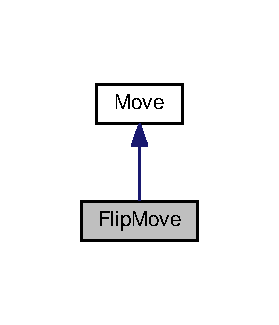
\includegraphics[width=134pt]{class_flip_move__inherit__graph}
\end{center}
\end{figure}


Collaboration diagram for Flip\-Move\-:\nopagebreak
\begin{figure}[H]
\begin{center}
\leavevmode
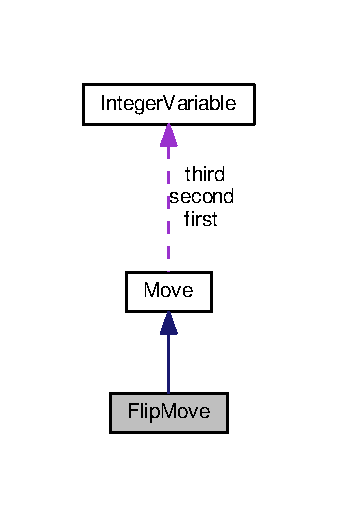
\includegraphics[width=162pt]{class_flip_move__coll__graph}
\end{center}
\end{figure}
\subsection*{Public Member Functions}
\begin{DoxyCompactItemize}
\item 
\hyperlink{class_flip_move_a31ec8ef20c4c96b1729092d1da02fe3e}{Flip\-Move} (\hyperlink{class_integer_variable}{Integer\-Variable} $\ast$iv)
\item 
\hyperlink{class_flip_move_a09277644ca1bae49d508646b05a6d064}{Flip\-Move} (const \hyperlink{class_flip_move}{Flip\-Move} \&orig)
\item 
virtual \hyperlink{class_flip_move_a9860e1365a6e9ab60b8de4265fe153ec}{$\sim$\-Flip\-Move} ()
\item 
\hyperlink{class_flip_move}{Flip\-Move} \& \hyperlink{class_flip_move_adda4f1374acf2a10425e86205df2d260}{operator=} (const \hyperlink{class_flip_move}{Flip\-Move} \&a)
\end{DoxyCompactItemize}
\subsection*{Additional Inherited Members}


\subsection{Constructor \& Destructor Documentation}
\hypertarget{class_flip_move_a31ec8ef20c4c96b1729092d1da02fe3e}{\index{Flip\-Move@{Flip\-Move}!Flip\-Move@{Flip\-Move}}
\index{Flip\-Move@{Flip\-Move}!FlipMove@{Flip\-Move}}
\subsubsection[{Flip\-Move}]{\setlength{\rightskip}{0pt plus 5cm}Flip\-Move\-::\-Flip\-Move (
\begin{DoxyParamCaption}
\item[{{\bf Integer\-Variable} $\ast$}]{iv}
\end{DoxyParamCaption}
)}}\label{class_flip_move_a31ec8ef20c4c96b1729092d1da02fe3e}
\hypertarget{class_flip_move_a09277644ca1bae49d508646b05a6d064}{\index{Flip\-Move@{Flip\-Move}!Flip\-Move@{Flip\-Move}}
\index{Flip\-Move@{Flip\-Move}!FlipMove@{Flip\-Move}}
\subsubsection[{Flip\-Move}]{\setlength{\rightskip}{0pt plus 5cm}Flip\-Move\-::\-Flip\-Move (
\begin{DoxyParamCaption}
\item[{const {\bf Flip\-Move} \&}]{orig}
\end{DoxyParamCaption}
)}}\label{class_flip_move_a09277644ca1bae49d508646b05a6d064}
\hypertarget{class_flip_move_a9860e1365a6e9ab60b8de4265fe153ec}{\index{Flip\-Move@{Flip\-Move}!$\sim$\-Flip\-Move@{$\sim$\-Flip\-Move}}
\index{$\sim$\-Flip\-Move@{$\sim$\-Flip\-Move}!FlipMove@{Flip\-Move}}
\subsubsection[{$\sim$\-Flip\-Move}]{\setlength{\rightskip}{0pt plus 5cm}Flip\-Move\-::$\sim$\-Flip\-Move (
\begin{DoxyParamCaption}
{}
\end{DoxyParamCaption}
)\hspace{0.3cm}{\ttfamily [virtual]}}}\label{class_flip_move_a9860e1365a6e9ab60b8de4265fe153ec}


\subsection{Member Function Documentation}
\hypertarget{class_flip_move_adda4f1374acf2a10425e86205df2d260}{\index{Flip\-Move@{Flip\-Move}!operator=@{operator=}}
\index{operator=@{operator=}!FlipMove@{Flip\-Move}}
\subsubsection[{operator=}]{\setlength{\rightskip}{0pt plus 5cm}Flip\-Move\-::operator= (
\begin{DoxyParamCaption}
\item[{const {\bf Flip\-Move} \&}]{a}
\end{DoxyParamCaption}
)}}\label{class_flip_move_adda4f1374acf2a10425e86205df2d260}


The documentation for this class was generated from the following files\-:\begin{DoxyCompactItemize}
\item 
\hyperlink{_flip_move_8hpp}{Flip\-Move.\-hpp}\item 
\hyperlink{_flip_move_8cpp}{Flip\-Move.\-cpp}\end{DoxyCompactItemize}

\hypertarget{class_gecode_solver}{\section{Gecode\-Solver Class Reference}
\label{class_gecode_solver}\index{Gecode\-Solver@{Gecode\-Solver}}
}


{\ttfamily \#include $<$Gecode\-Solver.\-hpp$>$}



Inheritance diagram for Gecode\-Solver\-:\nopagebreak
\begin{figure}[H]
\begin{center}
\leavevmode
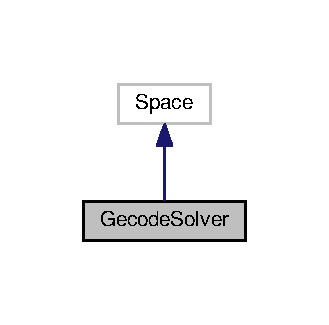
\includegraphics[width=158pt]{class_gecode_solver__inherit__graph}
\end{center}
\end{figure}


Collaboration diagram for Gecode\-Solver\-:\nopagebreak
\begin{figure}[H]
\begin{center}
\leavevmode
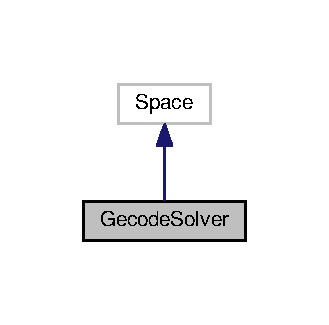
\includegraphics[width=158pt]{class_gecode_solver__coll__graph}
\end{center}
\end{figure}
\subsection*{Public Member Functions}
\begin{DoxyCompactItemize}
\item 
\hyperlink{class_gecode_solver_a79cd5fe79ac280dbc2d08a19552e22b7}{Gecode\-Solver} (std\-::shared\-\_\-ptr$<$ \hyperlink{class_model}{Model} $>$ \hyperlink{class_gecode_solver_a76210bf2a7eda291bf319971c0285fad}{model})
\item 
virtual \hyperlink{class_gecode_solver_aca5782c9a916038f0c59188508b0c703}{$\sim$\-Gecode\-Solver} ()
\item 
void \hyperlink{class_gecode_solver_aa3993533d534a437124fd75d2ab82425}{branch} ()
\item 
bool \hyperlink{class_gecode_solver_a3448f02748ee295111ded23cf90d6432}{initialize} (int Time\-For\-Gecode, bool fix)
\item 
bool \hyperlink{class_gecode_solver_a3c76a8f136a709f6984d23f399e6df3d}{Find\-Solution} (int Time\-For\-Gecode, bool fix)
\item 
void \hyperlink{class_gecode_solver_aa3fdaf0ff92e99bf1dd860d07cbac476}{linear} (std\-::vector$<$ int $>$ \&coefficients, const std\-::vector$<$ \hyperlink{class_integer_variable}{Integer\-Variable} $\ast$ $>$ \&variables, int relation, int upperbound)
\item 
void \hyperlink{class_gecode_solver_abcc193eafcc56a9b2a016c5831aaba9b}{create\-Gecode\-Variable} (int lb, int ub)
\item 
void \hyperlink{class_gecode_solver_a2e5913170cc34f8dca9eefd59448b5fe}{Set\-Values} (Gecode\-::\-Int\-Var\-Array vars)
\item 
void \hyperlink{class_gecode_solver_ad6198e37b78ec02a209d3e1f1bd6c929}{fix\-Variables} ()
\item 
void \hyperlink{class_gecode_solver_a768bbd3433d5c117fee99fcb554c87f5}{print\-Space\-Status} ()
\item 
void \hyperlink{class_gecode_solver_a8d16b569596eea5f47593ff03081025f}{create\-Array} ()
\item 
void \hyperlink{class_gecode_solver_a467af2791eed920c71e20b04e3d1c9c7}{print\-\_\-stats} (Gecode\-::\-Search\-::\-Statistics \&stat)
\item 
void \hyperlink{class_gecode_solver_a98286c7c09071746fc56e2e72175e0eb}{print} (std\-::ostream \&os) const 
\item 
\hyperlink{class_gecode_solver_a2215c9143fdfc572effa82a0764515dd}{Gecode\-Solver} (bool share, \hyperlink{class_gecode_solver}{Gecode\-Solver} \&s)
\item 
void \hyperlink{class_gecode_solver_ae9c28efac68fd3a7758078f3d859d821}{post\-Cov\-Sol} ()
\item 
virtual Space $\ast$ \hyperlink{class_gecode_solver_ac096dd0516b86a4aa290a8403aa56c5b}{copy} (bool share)
\end{DoxyCompactItemize}
\subsection*{Protected Attributes}
\begin{DoxyCompactItemize}
\item 
std\-::shared\-\_\-ptr$<$ \hyperlink{class_model}{Model} $>$ \hyperlink{class_gecode_solver_a76210bf2a7eda291bf319971c0285fad}{model}
\item 
Gecode\-::\-Int\-Var\-Array \hyperlink{class_gecode_solver_a17b5ac1b80ff807b0125ab423349a8a7}{Int\-Vars}
\item 
Gecode\-::\-Int\-Var\-Args \hyperlink{class_gecode_solver_a33b7c4b99d9be855c3275dad28b6a3e8}{tmp\-Vars}
\item 
Gecode\-::\-Int\-Var\-Args \hyperlink{class_gecode_solver_a73bb93a4cde21cd0fab60c73cf9cec0f}{bin\-Vars}
\end{DoxyCompactItemize}


\subsection{Constructor \& Destructor Documentation}
\hypertarget{class_gecode_solver_a79cd5fe79ac280dbc2d08a19552e22b7}{\index{Gecode\-Solver@{Gecode\-Solver}!Gecode\-Solver@{Gecode\-Solver}}
\index{Gecode\-Solver@{Gecode\-Solver}!GecodeSolver@{Gecode\-Solver}}
\subsubsection[{Gecode\-Solver}]{\setlength{\rightskip}{0pt plus 5cm}Gecode\-Solver\-::\-Gecode\-Solver (
\begin{DoxyParamCaption}
\item[{std\-::shared\-\_\-ptr$<$ {\bf Model} $>$}]{model}
\end{DoxyParamCaption}
)}}\label{class_gecode_solver_a79cd5fe79ac280dbc2d08a19552e22b7}
\hypertarget{class_gecode_solver_aca5782c9a916038f0c59188508b0c703}{\index{Gecode\-Solver@{Gecode\-Solver}!$\sim$\-Gecode\-Solver@{$\sim$\-Gecode\-Solver}}
\index{$\sim$\-Gecode\-Solver@{$\sim$\-Gecode\-Solver}!GecodeSolver@{Gecode\-Solver}}
\subsubsection[{$\sim$\-Gecode\-Solver}]{\setlength{\rightskip}{0pt plus 5cm}Gecode\-Solver\-::$\sim$\-Gecode\-Solver (
\begin{DoxyParamCaption}
{}
\end{DoxyParamCaption}
)\hspace{0.3cm}{\ttfamily [virtual]}}}\label{class_gecode_solver_aca5782c9a916038f0c59188508b0c703}
\hypertarget{class_gecode_solver_a2215c9143fdfc572effa82a0764515dd}{\index{Gecode\-Solver@{Gecode\-Solver}!Gecode\-Solver@{Gecode\-Solver}}
\index{Gecode\-Solver@{Gecode\-Solver}!GecodeSolver@{Gecode\-Solver}}
\subsubsection[{Gecode\-Solver}]{\setlength{\rightskip}{0pt plus 5cm}Gecode\-Solver\-::\-Gecode\-Solver (
\begin{DoxyParamCaption}
\item[{bool}]{share, }
\item[{{\bf Gecode\-Solver} \&}]{s}
\end{DoxyParamCaption}
)}}\label{class_gecode_solver_a2215c9143fdfc572effa82a0764515dd}


\subsection{Member Function Documentation}
\hypertarget{class_gecode_solver_aa3993533d534a437124fd75d2ab82425}{\index{Gecode\-Solver@{Gecode\-Solver}!branch@{branch}}
\index{branch@{branch}!GecodeSolver@{Gecode\-Solver}}
\subsubsection[{branch}]{\setlength{\rightskip}{0pt plus 5cm}void Gecode\-Solver\-::branch (
\begin{DoxyParamCaption}
{}
\end{DoxyParamCaption}
)}}\label{class_gecode_solver_aa3993533d534a437124fd75d2ab82425}
\hypertarget{class_gecode_solver_ac096dd0516b86a4aa290a8403aa56c5b}{\index{Gecode\-Solver@{Gecode\-Solver}!copy@{copy}}
\index{copy@{copy}!GecodeSolver@{Gecode\-Solver}}
\subsubsection[{copy}]{\setlength{\rightskip}{0pt plus 5cm}Gecode\-::\-Space $\ast$ Gecode\-Solver\-::copy (
\begin{DoxyParamCaption}
\item[{bool}]{share}
\end{DoxyParamCaption}
)\hspace{0.3cm}{\ttfamily [virtual]}}}\label{class_gecode_solver_ac096dd0516b86a4aa290a8403aa56c5b}
\hypertarget{class_gecode_solver_a8d16b569596eea5f47593ff03081025f}{\index{Gecode\-Solver@{Gecode\-Solver}!create\-Array@{create\-Array}}
\index{create\-Array@{create\-Array}!GecodeSolver@{Gecode\-Solver}}
\subsubsection[{create\-Array}]{\setlength{\rightskip}{0pt plus 5cm}void Gecode\-Solver\-::create\-Array (
\begin{DoxyParamCaption}
{}
\end{DoxyParamCaption}
)}}\label{class_gecode_solver_a8d16b569596eea5f47593ff03081025f}
\hypertarget{class_gecode_solver_abcc193eafcc56a9b2a016c5831aaba9b}{\index{Gecode\-Solver@{Gecode\-Solver}!create\-Gecode\-Variable@{create\-Gecode\-Variable}}
\index{create\-Gecode\-Variable@{create\-Gecode\-Variable}!GecodeSolver@{Gecode\-Solver}}
\subsubsection[{create\-Gecode\-Variable}]{\setlength{\rightskip}{0pt plus 5cm}void Gecode\-Solver\-::create\-Gecode\-Variable (
\begin{DoxyParamCaption}
\item[{int}]{lb, }
\item[{int}]{ub}
\end{DoxyParamCaption}
)}}\label{class_gecode_solver_abcc193eafcc56a9b2a016c5831aaba9b}
\hypertarget{class_gecode_solver_a3c76a8f136a709f6984d23f399e6df3d}{\index{Gecode\-Solver@{Gecode\-Solver}!Find\-Solution@{Find\-Solution}}
\index{Find\-Solution@{Find\-Solution}!GecodeSolver@{Gecode\-Solver}}
\subsubsection[{Find\-Solution}]{\setlength{\rightskip}{0pt plus 5cm}bool Gecode\-Solver\-::\-Find\-Solution (
\begin{DoxyParamCaption}
\item[{int}]{Time\-For\-Gecode, }
\item[{bool}]{fix}
\end{DoxyParamCaption}
)}}\label{class_gecode_solver_a3c76a8f136a709f6984d23f399e6df3d}
\hypertarget{class_gecode_solver_ad6198e37b78ec02a209d3e1f1bd6c929}{\index{Gecode\-Solver@{Gecode\-Solver}!fix\-Variables@{fix\-Variables}}
\index{fix\-Variables@{fix\-Variables}!GecodeSolver@{Gecode\-Solver}}
\subsubsection[{fix\-Variables}]{\setlength{\rightskip}{0pt plus 5cm}void Gecode\-Solver\-::fix\-Variables (
\begin{DoxyParamCaption}
{}
\end{DoxyParamCaption}
)}}\label{class_gecode_solver_ad6198e37b78ec02a209d3e1f1bd6c929}
\hypertarget{class_gecode_solver_a3448f02748ee295111ded23cf90d6432}{\index{Gecode\-Solver@{Gecode\-Solver}!initialize@{initialize}}
\index{initialize@{initialize}!GecodeSolver@{Gecode\-Solver}}
\subsubsection[{initialize}]{\setlength{\rightskip}{0pt plus 5cm}bool Gecode\-Solver\-::initialize (
\begin{DoxyParamCaption}
\item[{int}]{Time\-For\-Gecode, }
\item[{bool}]{fix}
\end{DoxyParamCaption}
)}}\label{class_gecode_solver_a3448f02748ee295111ded23cf90d6432}
\hypertarget{class_gecode_solver_aa3fdaf0ff92e99bf1dd860d07cbac476}{\index{Gecode\-Solver@{Gecode\-Solver}!linear@{linear}}
\index{linear@{linear}!GecodeSolver@{Gecode\-Solver}}
\subsubsection[{linear}]{\setlength{\rightskip}{0pt plus 5cm}void Gecode\-Solver\-::linear (
\begin{DoxyParamCaption}
\item[{std\-::vector$<$ int $>$ \&}]{coefficients, }
\item[{const std\-::vector$<$ {\bf Integer\-Variable} $\ast$ $>$ \&}]{variables, }
\item[{int}]{relation, }
\item[{int}]{upperbound}
\end{DoxyParamCaption}
)}}\label{class_gecode_solver_aa3fdaf0ff92e99bf1dd860d07cbac476}
\hypertarget{class_gecode_solver_ae9c28efac68fd3a7758078f3d859d821}{\index{Gecode\-Solver@{Gecode\-Solver}!post\-Cov\-Sol@{post\-Cov\-Sol}}
\index{post\-Cov\-Sol@{post\-Cov\-Sol}!GecodeSolver@{Gecode\-Solver}}
\subsubsection[{post\-Cov\-Sol}]{\setlength{\rightskip}{0pt plus 5cm}void Gecode\-Solver\-::post\-Cov\-Sol (
\begin{DoxyParamCaption}
{}
\end{DoxyParamCaption}
)}}\label{class_gecode_solver_ae9c28efac68fd3a7758078f3d859d821}
\hypertarget{class_gecode_solver_a98286c7c09071746fc56e2e72175e0eb}{\index{Gecode\-Solver@{Gecode\-Solver}!print@{print}}
\index{print@{print}!GecodeSolver@{Gecode\-Solver}}
\subsubsection[{print}]{\setlength{\rightskip}{0pt plus 5cm}void Gecode\-Solver\-::print (
\begin{DoxyParamCaption}
\item[{std\-::ostream \&}]{os}
\end{DoxyParamCaption}
) const}}\label{class_gecode_solver_a98286c7c09071746fc56e2e72175e0eb}
\hypertarget{class_gecode_solver_a467af2791eed920c71e20b04e3d1c9c7}{\index{Gecode\-Solver@{Gecode\-Solver}!print\-\_\-stats@{print\-\_\-stats}}
\index{print\-\_\-stats@{print\-\_\-stats}!GecodeSolver@{Gecode\-Solver}}
\subsubsection[{print\-\_\-stats}]{\setlength{\rightskip}{0pt plus 5cm}void Gecode\-Solver\-::print\-\_\-stats (
\begin{DoxyParamCaption}
\item[{Gecode\-::\-Search\-::\-Statistics \&}]{stat}
\end{DoxyParamCaption}
)}}\label{class_gecode_solver_a467af2791eed920c71e20b04e3d1c9c7}
\hypertarget{class_gecode_solver_a768bbd3433d5c117fee99fcb554c87f5}{\index{Gecode\-Solver@{Gecode\-Solver}!print\-Space\-Status@{print\-Space\-Status}}
\index{print\-Space\-Status@{print\-Space\-Status}!GecodeSolver@{Gecode\-Solver}}
\subsubsection[{print\-Space\-Status}]{\setlength{\rightskip}{0pt plus 5cm}void Gecode\-Solver\-::print\-Space\-Status (
\begin{DoxyParamCaption}
{}
\end{DoxyParamCaption}
)}}\label{class_gecode_solver_a768bbd3433d5c117fee99fcb554c87f5}
\hypertarget{class_gecode_solver_a2e5913170cc34f8dca9eefd59448b5fe}{\index{Gecode\-Solver@{Gecode\-Solver}!Set\-Values@{Set\-Values}}
\index{Set\-Values@{Set\-Values}!GecodeSolver@{Gecode\-Solver}}
\subsubsection[{Set\-Values}]{\setlength{\rightskip}{0pt plus 5cm}void Gecode\-Solver\-::\-Set\-Values (
\begin{DoxyParamCaption}
\item[{Gecode\-::\-Int\-Var\-Array}]{vars}
\end{DoxyParamCaption}
)}}\label{class_gecode_solver_a2e5913170cc34f8dca9eefd59448b5fe}


\subsection{Member Data Documentation}
\hypertarget{class_gecode_solver_a73bb93a4cde21cd0fab60c73cf9cec0f}{\index{Gecode\-Solver@{Gecode\-Solver}!bin\-Vars@{bin\-Vars}}
\index{bin\-Vars@{bin\-Vars}!GecodeSolver@{Gecode\-Solver}}
\subsubsection[{bin\-Vars}]{\setlength{\rightskip}{0pt plus 5cm}Gecode\-::\-Int\-Var\-Args Gecode\-Solver\-::bin\-Vars\hspace{0.3cm}{\ttfamily [protected]}}}\label{class_gecode_solver_a73bb93a4cde21cd0fab60c73cf9cec0f}
\hypertarget{class_gecode_solver_a17b5ac1b80ff807b0125ab423349a8a7}{\index{Gecode\-Solver@{Gecode\-Solver}!Int\-Vars@{Int\-Vars}}
\index{Int\-Vars@{Int\-Vars}!GecodeSolver@{Gecode\-Solver}}
\subsubsection[{Int\-Vars}]{\setlength{\rightskip}{0pt plus 5cm}Gecode\-::\-Int\-Var\-Array Gecode\-Solver\-::\-Int\-Vars\hspace{0.3cm}{\ttfamily [protected]}}}\label{class_gecode_solver_a17b5ac1b80ff807b0125ab423349a8a7}
\hypertarget{class_gecode_solver_a76210bf2a7eda291bf319971c0285fad}{\index{Gecode\-Solver@{Gecode\-Solver}!model@{model}}
\index{model@{model}!GecodeSolver@{Gecode\-Solver}}
\subsubsection[{model}]{\setlength{\rightskip}{0pt plus 5cm}std\-::shared\-\_\-ptr$<${\bf Model}$>$ Gecode\-Solver\-::model\hspace{0.3cm}{\ttfamily [protected]}}}\label{class_gecode_solver_a76210bf2a7eda291bf319971c0285fad}
\hypertarget{class_gecode_solver_a33b7c4b99d9be855c3275dad28b6a3e8}{\index{Gecode\-Solver@{Gecode\-Solver}!tmp\-Vars@{tmp\-Vars}}
\index{tmp\-Vars@{tmp\-Vars}!GecodeSolver@{Gecode\-Solver}}
\subsubsection[{tmp\-Vars}]{\setlength{\rightskip}{0pt plus 5cm}Gecode\-::\-Int\-Var\-Args Gecode\-Solver\-::tmp\-Vars\hspace{0.3cm}{\ttfamily [protected]}}}\label{class_gecode_solver_a33b7c4b99d9be855c3275dad28b6a3e8}


The documentation for this class was generated from the following files\-:\begin{DoxyCompactItemize}
\item 
\hyperlink{_gecode_solver_8hpp}{Gecode\-Solver.\-hpp}\item 
\hyperlink{_gecode_solver_8cpp}{Gecode\-Solver.\-cpp}\end{DoxyCompactItemize}

\hypertarget{class_general_solver}{\section{General\-Solver Class Reference}
\label{class_general_solver}\index{General\-Solver@{General\-Solver}}
}


{\ttfamily \#include $<$General\-Solver.\-hpp$>$}



Inheritance diagram for General\-Solver\-:\nopagebreak
\begin{figure}[H]
\begin{center}
\leavevmode
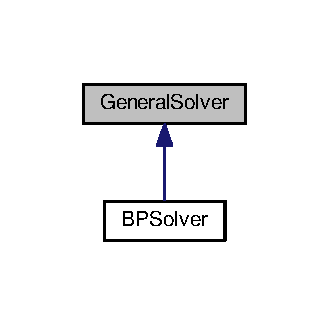
\includegraphics[width=158pt]{class_general_solver__inherit__graph}
\end{center}
\end{figure}
\subsection*{Public Member Functions}
\begin{DoxyCompactItemize}
\item 
\hyperlink{class_general_solver_af6a162313c6ca4252b3fb09335e44add}{General\-Solver} ()
\item 
\hyperlink{class_general_solver_adca6fe5293d5216c11b82313a6684c44}{$\sim$\-General\-Solver} ()
\item 
\hyperlink{class_general_solver}{General\-Solver} \& \hyperlink{class_general_solver_a39fa8b0891ddd2a84d07e08e781c560a}{operator=} (const \hyperlink{class_general_solver}{General\-Solver} \&a)
\item 
void \hyperlink{class_general_solver_aa431b9e98724dde0d6c6cbe850f9e801}{linear} (std\-::vector$<$ int $>$ \&coefficients, std\-::vector$<$ \hyperlink{class_integer_variable}{Integer\-Variable} $\ast$ $>$ \&variables, int relation, int ub, unsigned priority)
\item 
void \hyperlink{class_general_solver_a11f08371a72b67b40e72822ac15bfd69}{create\-Int\-Vars} (unsigned number\-Of\-Variables, int lb, int ub)
\item 
void \hyperlink{class_general_solver_a0aef6a5662ed6cc2b87a04959221c0e4}{create\-Int\-Var} (int lb, int ub)
\begin{DoxyCompactList}\small\item\em Create a single variable with given lower and upper bound. \end{DoxyCompactList}\item 
std\-::vector$<$ \hyperlink{class_integer_variable}{Integer\-Variable} $\ast$ $>$ \& \hyperlink{class_general_solver_a0ca7cec1b92600361e1b7d4aeefa4d20}{get\-All\-Variables} ()
\item 
void \hyperlink{class_general_solver_a35a41c86b56b652bb8c6b7b96a4e8713}{print} (std\-::vector$<$ \hyperlink{class_integer_variable}{Integer\-Variable} $>$ \&Integer\-Variables)
\begin{DoxyCompactList}\small\item\em Only for testing, should be removed. \end{DoxyCompactList}\item 
void \hyperlink{class_general_solver_a8da2ce27fc096edaee250ea3ed068072}{Initial\-Solution} (int Time\-For\-Gecode)
\item 
void \hyperlink{class_general_solver_a3ab6827d7643be316d88e689845b86ec}{relax} (int times\-Relaxed)
\item 
void \hyperlink{class_general_solver_ac8980bcadaf659185f8d1f253e000239}{simple\-Relax} (int times\-Relaxed)
\item 
void \hyperlink{class_general_solver_a2b0f1c903cb82da4dc365c54f99f7dc7}{initialize\-L\-S} ()
\item 
bool \hyperlink{class_general_solver_ad33424f327d023dbd9036f6c00d67016}{can\-Be\-Made\-Oneway} (\hyperlink{class_integer_variable}{Integer\-Variable} $\ast$iv, \hyperlink{_constants_8hpp_ab3a9f5ca3242dd173f530bb9f68fc611}{constraint} cons)
\item 
void \hyperlink{class_general_solver_a791480a81d20c730b3922626b17ef86a}{make\-Oneway} (\hyperlink{class_integer_variable}{Integer\-Variable} $\ast$iv, \hyperlink{_constants_8hpp_ab3a9f5ca3242dd173f530bb9f68fc611}{constraint} cons, int coeff)
\item 
int \hyperlink{class_general_solver_a26335b71277441fd0231e6d59f0da504}{get\-Initial\-Value} ()
\item 
void \hyperlink{class_general_solver_a9450eca3384912647dc14542daff80d0}{optimize\-Solution} (int time)
\item 
void \hyperlink{class_general_solver_ae3a2883d94de6f10d13c815a500e515a}{print\-Current} ()
\end{DoxyCompactItemize}
\subsection*{Private Member Functions}
\begin{DoxyCompactItemize}
\item 
void \hyperlink{class_general_solver_a5dc280bd7c1d8527f3127147faf885d0}{print\-\_\-stats} (Gecode\-::\-Search\-::\-Statistics \&stat)
\end{DoxyCompactItemize}
\subsection*{Private Attributes}
\begin{DoxyCompactItemize}
\item 
std\-::shared\-\_\-ptr$<$ \hyperlink{class_model}{Model} $>$ \hyperlink{class_general_solver_a83831a1f3765851d544a8badccab3178}{model} = std\-::make\-\_\-shared$<$\hyperlink{class_model}{Model}$>$ ()
\item 
std\-::shared\-\_\-ptr$<$ \hyperlink{class_state}{State} $>$ \hyperlink{class_general_solver_aa8f7806985c11c39b355f0720764ce66}{st} = std\-::make\-\_\-shared$<$\hyperlink{class_state}{State}$>$(\hyperlink{class_general_solver_a83831a1f3765851d544a8badccab3178}{model})
\item 
std\-::unique\-\_\-ptr$<$ \hyperlink{class_l_s_space}{L\-S\-Space} $>$ \hyperlink{class_general_solver_ad70adfee5b2c8779c975d91cb24efcc5}{L\-S} = std\-::unique\-\_\-ptr$<$\hyperlink{class_l_s_space}{L\-S\-Space}$>$ (new \hyperlink{class_l_s_space}{L\-S\-Space}(\hyperlink{class_general_solver_a83831a1f3765851d544a8badccab3178}{model}))
\item 
std\-::unique\-\_\-ptr$<$ \hyperlink{class_gecode_solver}{Gecode\-Solver} $>$ \hyperlink{class_general_solver_a7edfe7eb7a5b8c492e2aa4b697959a3e}{G\-S} = std\-::unique\-\_\-ptr$<$\hyperlink{class_gecode_solver}{Gecode\-Solver}$>$ (new \hyperlink{class_gecode_solver}{Gecode\-Solver}(\hyperlink{class_general_solver_a83831a1f3765851d544a8badccab3178}{model}))
\end{DoxyCompactItemize}
\subsection*{Friends}
\begin{DoxyCompactItemize}
\item 
class \hyperlink{class_general_solver_a5b78b1c2e1fa07ffed92da365593eaa4}{Test}
\end{DoxyCompactItemize}


\subsection{Constructor \& Destructor Documentation}
\hypertarget{class_general_solver_af6a162313c6ca4252b3fb09335e44add}{\index{General\-Solver@{General\-Solver}!General\-Solver@{General\-Solver}}
\index{General\-Solver@{General\-Solver}!GeneralSolver@{General\-Solver}}
\subsubsection[{General\-Solver}]{\setlength{\rightskip}{0pt plus 5cm}General\-Solver\-::\-General\-Solver (
\begin{DoxyParamCaption}
{}
\end{DoxyParamCaption}
)\hspace{0.3cm}{\ttfamily [inline]}}}\label{class_general_solver_af6a162313c6ca4252b3fb09335e44add}
\hypertarget{class_general_solver_adca6fe5293d5216c11b82313a6684c44}{\index{General\-Solver@{General\-Solver}!$\sim$\-General\-Solver@{$\sim$\-General\-Solver}}
\index{$\sim$\-General\-Solver@{$\sim$\-General\-Solver}!GeneralSolver@{General\-Solver}}
\subsubsection[{$\sim$\-General\-Solver}]{\setlength{\rightskip}{0pt plus 5cm}General\-Solver\-::$\sim$\-General\-Solver (
\begin{DoxyParamCaption}
{}
\end{DoxyParamCaption}
)\hspace{0.3cm}{\ttfamily [inline]}}}\label{class_general_solver_adca6fe5293d5216c11b82313a6684c44}


\subsection{Member Function Documentation}
\hypertarget{class_general_solver_ad33424f327d023dbd9036f6c00d67016}{\index{General\-Solver@{General\-Solver}!can\-Be\-Made\-Oneway@{can\-Be\-Made\-Oneway}}
\index{can\-Be\-Made\-Oneway@{can\-Be\-Made\-Oneway}!GeneralSolver@{General\-Solver}}
\subsubsection[{can\-Be\-Made\-Oneway}]{\setlength{\rightskip}{0pt plus 5cm}bool General\-Solver\-::can\-Be\-Made\-Oneway (
\begin{DoxyParamCaption}
\item[{{\bf Integer\-Variable} $\ast$}]{iv, }
\item[{{\bf constraint}}]{cons}
\end{DoxyParamCaption}
)\hspace{0.3cm}{\ttfamily [inline]}}}\label{class_general_solver_ad33424f327d023dbd9036f6c00d67016}
\hypertarget{class_general_solver_a0aef6a5662ed6cc2b87a04959221c0e4}{\index{General\-Solver@{General\-Solver}!create\-Int\-Var@{create\-Int\-Var}}
\index{create\-Int\-Var@{create\-Int\-Var}!GeneralSolver@{General\-Solver}}
\subsubsection[{create\-Int\-Var}]{\setlength{\rightskip}{0pt plus 5cm}void General\-Solver\-::create\-Int\-Var (
\begin{DoxyParamCaption}
\item[{int}]{lb, }
\item[{int}]{ub}
\end{DoxyParamCaption}
)\hspace{0.3cm}{\ttfamily [inline]}}}\label{class_general_solver_a0aef6a5662ed6cc2b87a04959221c0e4}


Create a single variable with given lower and upper bound. 

\hypertarget{class_general_solver_a11f08371a72b67b40e72822ac15bfd69}{\index{General\-Solver@{General\-Solver}!create\-Int\-Vars@{create\-Int\-Vars}}
\index{create\-Int\-Vars@{create\-Int\-Vars}!GeneralSolver@{General\-Solver}}
\subsubsection[{create\-Int\-Vars}]{\setlength{\rightskip}{0pt plus 5cm}void General\-Solver\-::create\-Int\-Vars (
\begin{DoxyParamCaption}
\item[{unsigned}]{number\-Of\-Variables, }
\item[{int}]{lb, }
\item[{int}]{ub}
\end{DoxyParamCaption}
)\hspace{0.3cm}{\ttfamily [inline]}}}\label{class_general_solver_a11f08371a72b67b40e72822ac15bfd69}
\hypertarget{class_general_solver_a0ca7cec1b92600361e1b7d4aeefa4d20}{\index{General\-Solver@{General\-Solver}!get\-All\-Variables@{get\-All\-Variables}}
\index{get\-All\-Variables@{get\-All\-Variables}!GeneralSolver@{General\-Solver}}
\subsubsection[{get\-All\-Variables}]{\setlength{\rightskip}{0pt plus 5cm}std\-::vector$<${\bf Integer\-Variable}$\ast$$>$\& General\-Solver\-::get\-All\-Variables (
\begin{DoxyParamCaption}
{}
\end{DoxyParamCaption}
)\hspace{0.3cm}{\ttfamily [inline]}}}\label{class_general_solver_a0ca7cec1b92600361e1b7d4aeefa4d20}
\hypertarget{class_general_solver_a26335b71277441fd0231e6d59f0da504}{\index{General\-Solver@{General\-Solver}!get\-Initial\-Value@{get\-Initial\-Value}}
\index{get\-Initial\-Value@{get\-Initial\-Value}!GeneralSolver@{General\-Solver}}
\subsubsection[{get\-Initial\-Value}]{\setlength{\rightskip}{0pt plus 5cm}int General\-Solver\-::get\-Initial\-Value (
\begin{DoxyParamCaption}
{}
\end{DoxyParamCaption}
)\hspace{0.3cm}{\ttfamily [inline]}}}\label{class_general_solver_a26335b71277441fd0231e6d59f0da504}
\hypertarget{class_general_solver_a2b0f1c903cb82da4dc365c54f99f7dc7}{\index{General\-Solver@{General\-Solver}!initialize\-L\-S@{initialize\-L\-S}}
\index{initialize\-L\-S@{initialize\-L\-S}!GeneralSolver@{General\-Solver}}
\subsubsection[{initialize\-L\-S}]{\setlength{\rightskip}{0pt plus 5cm}void General\-Solver\-::initialize\-L\-S (
\begin{DoxyParamCaption}
{}
\end{DoxyParamCaption}
)\hspace{0.3cm}{\ttfamily [inline]}}}\label{class_general_solver_a2b0f1c903cb82da4dc365c54f99f7dc7}
Sort constraints a variable is part of in decreasing order according to domain

Sort integer variables decreasing order according to number of constraints they are involved

Omskriv det hele. Alt skal bygges op model-\/$>$invariant fungerer som en prioritet invariant skal opdateres i. Hver variable har deres egen kø. \hypertarget{class_general_solver_a8da2ce27fc096edaee250ea3ed068072}{\index{General\-Solver@{General\-Solver}!Initial\-Solution@{Initial\-Solution}}
\index{Initial\-Solution@{Initial\-Solution}!GeneralSolver@{General\-Solver}}
\subsubsection[{Initial\-Solution}]{\setlength{\rightskip}{0pt plus 5cm}void General\-Solver\-::\-Initial\-Solution (
\begin{DoxyParamCaption}
\item[{int}]{Time\-For\-Gecode}
\end{DoxyParamCaption}
)\hspace{0.3cm}{\ttfamily [inline]}}}\label{class_general_solver_a8da2ce27fc096edaee250ea3ed068072}
Uses Gecode to find initial solution returns a new \hyperlink{class_general_solver}{General\-Solver} with the initial solution the old (the one this method is called from) is not updated with new solution. \hypertarget{class_general_solver_aa431b9e98724dde0d6c6cbe850f9e801}{\index{General\-Solver@{General\-Solver}!linear@{linear}}
\index{linear@{linear}!GeneralSolver@{General\-Solver}}
\subsubsection[{linear}]{\setlength{\rightskip}{0pt plus 5cm}void General\-Solver\-::linear (
\begin{DoxyParamCaption}
\item[{std\-::vector$<$ int $>$ \&}]{coefficients, }
\item[{std\-::vector$<$ {\bf Integer\-Variable} $\ast$ $>$ \&}]{variables, }
\item[{int}]{relation, }
\item[{int}]{ub, }
\item[{unsigned}]{priority}
\end{DoxyParamCaption}
)\hspace{0.3cm}{\ttfamily [inline]}}}\label{class_general_solver_aa431b9e98724dde0d6c6cbe850f9e801}
\hypertarget{class_general_solver_a791480a81d20c730b3922626b17ef86a}{\index{General\-Solver@{General\-Solver}!make\-Oneway@{make\-Oneway}}
\index{make\-Oneway@{make\-Oneway}!GeneralSolver@{General\-Solver}}
\subsubsection[{make\-Oneway}]{\setlength{\rightskip}{0pt plus 5cm}void General\-Solver\-::make\-Oneway (
\begin{DoxyParamCaption}
\item[{{\bf Integer\-Variable} $\ast$}]{iv, }
\item[{{\bf constraint}}]{cons, }
\item[{int}]{coeff}
\end{DoxyParamCaption}
)\hspace{0.3cm}{\ttfamily [inline]}}}\label{class_general_solver_a791480a81d20c730b3922626b17ef86a}
\hypertarget{class_general_solver_a39fa8b0891ddd2a84d07e08e781c560a}{\index{General\-Solver@{General\-Solver}!operator=@{operator=}}
\index{operator=@{operator=}!GeneralSolver@{General\-Solver}}
\subsubsection[{operator=}]{\setlength{\rightskip}{0pt plus 5cm}{\bf General\-Solver}\& General\-Solver\-::operator= (
\begin{DoxyParamCaption}
\item[{const {\bf General\-Solver} \&}]{a}
\end{DoxyParamCaption}
)\hspace{0.3cm}{\ttfamily [inline]}}}\label{class_general_solver_a39fa8b0891ddd2a84d07e08e781c560a}
\hypertarget{class_general_solver_a9450eca3384912647dc14542daff80d0}{\index{General\-Solver@{General\-Solver}!optimize\-Solution@{optimize\-Solution}}
\index{optimize\-Solution@{optimize\-Solution}!GeneralSolver@{General\-Solver}}
\subsubsection[{optimize\-Solution}]{\setlength{\rightskip}{0pt plus 5cm}void General\-Solver\-::optimize\-Solution (
\begin{DoxyParamCaption}
\item[{int}]{time}
\end{DoxyParamCaption}
)\hspace{0.3cm}{\ttfamily [inline]}}}\label{class_general_solver_a9450eca3384912647dc14542daff80d0}
\hypertarget{class_general_solver_a35a41c86b56b652bb8c6b7b96a4e8713}{\index{General\-Solver@{General\-Solver}!print@{print}}
\index{print@{print}!GeneralSolver@{General\-Solver}}
\subsubsection[{print}]{\setlength{\rightskip}{0pt plus 5cm}void General\-Solver\-::print (
\begin{DoxyParamCaption}
\item[{std\-::vector$<$ {\bf Integer\-Variable} $>$ \&}]{Integer\-Variables}
\end{DoxyParamCaption}
)\hspace{0.3cm}{\ttfamily [inline]}}}\label{class_general_solver_a35a41c86b56b652bb8c6b7b96a4e8713}


Only for testing, should be removed. 

\hypertarget{class_general_solver_a5dc280bd7c1d8527f3127147faf885d0}{\index{General\-Solver@{General\-Solver}!print\-\_\-stats@{print\-\_\-stats}}
\index{print\-\_\-stats@{print\-\_\-stats}!GeneralSolver@{General\-Solver}}
\subsubsection[{print\-\_\-stats}]{\setlength{\rightskip}{0pt plus 5cm}void General\-Solver\-::print\-\_\-stats (
\begin{DoxyParamCaption}
\item[{Gecode\-::\-Search\-::\-Statistics \&}]{stat}
\end{DoxyParamCaption}
)\hspace{0.3cm}{\ttfamily [inline]}, {\ttfamily [private]}}}\label{class_general_solver_a5dc280bd7c1d8527f3127147faf885d0}
\hypertarget{class_general_solver_ae3a2883d94de6f10d13c815a500e515a}{\index{General\-Solver@{General\-Solver}!print\-Current@{print\-Current}}
\index{print\-Current@{print\-Current}!GeneralSolver@{General\-Solver}}
\subsubsection[{print\-Current}]{\setlength{\rightskip}{0pt plus 5cm}void General\-Solver\-::print\-Current (
\begin{DoxyParamCaption}
{}
\end{DoxyParamCaption}
)\hspace{0.3cm}{\ttfamily [inline]}}}\label{class_general_solver_ae3a2883d94de6f10d13c815a500e515a}
\hypertarget{class_general_solver_a3ab6827d7643be316d88e689845b86ec}{\index{General\-Solver@{General\-Solver}!relax@{relax}}
\index{relax@{relax}!GeneralSolver@{General\-Solver}}
\subsubsection[{relax}]{\setlength{\rightskip}{0pt plus 5cm}void General\-Solver\-::relax (
\begin{DoxyParamCaption}
\item[{int}]{times\-Relaxed}
\end{DoxyParamCaption}
)\hspace{0.3cm}{\ttfamily [inline]}}}\label{class_general_solver_a3ab6827d7643be316d88e689845b86ec}
relaxes the space (reduce the number of constraints). Used when Gecode cant find a solution in time. Only works for binary Different relaxation can be chosen (not atm) needs to create a new \hyperlink{class_gecode_solver}{Gecode\-Solver} (Space) and recreate some of the calls the user made (those that should not be relaxed). \hypertarget{class_general_solver_ac8980bcadaf659185f8d1f253e000239}{\index{General\-Solver@{General\-Solver}!simple\-Relax@{simple\-Relax}}
\index{simple\-Relax@{simple\-Relax}!GeneralSolver@{General\-Solver}}
\subsubsection[{simple\-Relax}]{\setlength{\rightskip}{0pt plus 5cm}void General\-Solver\-::simple\-Relax (
\begin{DoxyParamCaption}
\item[{int}]{times\-Relaxed}
\end{DoxyParamCaption}
)\hspace{0.3cm}{\ttfamily [inline]}}}\label{class_general_solver_ac8980bcadaf659185f8d1f253e000239}


\subsection{Friends And Related Function Documentation}
\hypertarget{class_general_solver_a5b78b1c2e1fa07ffed92da365593eaa4}{\index{General\-Solver@{General\-Solver}!Test@{Test}}
\index{Test@{Test}!GeneralSolver@{General\-Solver}}
\subsubsection[{Test}]{\setlength{\rightskip}{0pt plus 5cm}friend class Test\hspace{0.3cm}{\ttfamily [friend]}}}\label{class_general_solver_a5b78b1c2e1fa07ffed92da365593eaa4}


\subsection{Member Data Documentation}
\hypertarget{class_general_solver_a7edfe7eb7a5b8c492e2aa4b697959a3e}{\index{General\-Solver@{General\-Solver}!G\-S@{G\-S}}
\index{G\-S@{G\-S}!GeneralSolver@{General\-Solver}}
\subsubsection[{G\-S}]{\setlength{\rightskip}{0pt plus 5cm}std\-::unique\-\_\-ptr$<${\bf Gecode\-Solver}$>$ General\-Solver\-::\-G\-S = std\-::unique\-\_\-ptr$<${\bf Gecode\-Solver}$>$ (new {\bf Gecode\-Solver}({\bf model}))\hspace{0.3cm}{\ttfamily [private]}}}\label{class_general_solver_a7edfe7eb7a5b8c492e2aa4b697959a3e}
\hypertarget{class_general_solver_ad70adfee5b2c8779c975d91cb24efcc5}{\index{General\-Solver@{General\-Solver}!L\-S@{L\-S}}
\index{L\-S@{L\-S}!GeneralSolver@{General\-Solver}}
\subsubsection[{L\-S}]{\setlength{\rightskip}{0pt plus 5cm}std\-::unique\-\_\-ptr$<${\bf L\-S\-Space}$>$ General\-Solver\-::\-L\-S = std\-::unique\-\_\-ptr$<${\bf L\-S\-Space}$>$ (new {\bf L\-S\-Space}({\bf model}))\hspace{0.3cm}{\ttfamily [private]}}}\label{class_general_solver_ad70adfee5b2c8779c975d91cb24efcc5}
\hypertarget{class_general_solver_a83831a1f3765851d544a8badccab3178}{\index{General\-Solver@{General\-Solver}!model@{model}}
\index{model@{model}!GeneralSolver@{General\-Solver}}
\subsubsection[{model}]{\setlength{\rightskip}{0pt plus 5cm}std\-::shared\-\_\-ptr$<${\bf Model}$>$ General\-Solver\-::model = std\-::make\-\_\-shared$<${\bf Model}$>$ ()\hspace{0.3cm}{\ttfamily [private]}}}\label{class_general_solver_a83831a1f3765851d544a8badccab3178}
\hypertarget{class_general_solver_aa8f7806985c11c39b355f0720764ce66}{\index{General\-Solver@{General\-Solver}!st@{st}}
\index{st@{st}!GeneralSolver@{General\-Solver}}
\subsubsection[{st}]{\setlength{\rightskip}{0pt plus 5cm}std\-::shared\-\_\-ptr$<${\bf State}$>$ General\-Solver\-::st = std\-::make\-\_\-shared$<${\bf State}$>$({\bf model})\hspace{0.3cm}{\ttfamily [private]}}}\label{class_general_solver_aa8f7806985c11c39b355f0720764ce66}


The documentation for this class was generated from the following file\-:\begin{DoxyCompactItemize}
\item 
\hyperlink{_general_solver_8hpp}{General\-Solver.\-hpp}\end{DoxyCompactItemize}

\hypertarget{class_integer_variable}{\section{Integer\-Variable Class Reference}
\label{class_integer_variable}\index{Integer\-Variable@{Integer\-Variable}}
}


{\ttfamily \#include $<$Integer\-Variable.\-hpp$>$}

\subsection*{Public Member Functions}
\begin{DoxyCompactItemize}
\item 
\hyperlink{_constants_8hpp_a02baa5ed1a26d5d8a8c4adb2d0e59a57}{Variable\-In\-Constraints} \& \hyperlink{class_integer_variable_a5e9776b7de2cecf0c68a321908996240}{used\-In\-Constraints} ()
\item 
void \hyperlink{class_integer_variable_ac7d3b8458189707ec2bc30ed8223d476}{add\-To\-Used\-In\-Constraints} (std\-::shared\-\_\-ptr$<$ \hyperlink{class_constraint}{Constraint} $>$ \hyperlink{_constants_8hpp_ab3a9f5ca3242dd173f530bb9f68fc611}{constraint})
\item 
\hyperlink{_constants_8hpp_ac9b562f250a09412c017b68185321eba}{invariant} \hyperlink{class_integer_variable_a397ba35a4bae5508d4d44e164d02c2ac}{get\-Oneway} ()
\item 
void \hyperlink{class_integer_variable_abdaa77cb4582cf6db133ffb1a1cf839d}{set\-Defined\-By} (\hyperlink{_constants_8hpp_ac9b562f250a09412c017b68185321eba}{invariant} invar, \hyperlink{_constants_8hpp_ab3a9f5ca3242dd173f530bb9f68fc611}{constraint} cons)
\item 
\hyperlink{class_integer_variable_ae04ab8d89dbffd42c7bba04f0db31456}{Integer\-Variable} (int lowerbound, int upperbound, int id)
\item 
void \hyperlink{class_integer_variable_a6a1823e3601a6375b55b5cfc3112179d}{set\-Current\-Value} (int val)
\item 
bool \hyperlink{class_integer_variable_a773c5fa99af9215ba9a56f97ea25ed80}{is\-Integer\-Variable} ()
\item 
int \hyperlink{class_integer_variable_a31c31e2a2950e3a9f3cfd46c59485414}{get\-Current\-Value} ()
\item 
void \hyperlink{class_integer_variable_aad10aa4509149b887c26133af7f04fa0}{add\-To\-Update} (\hyperlink{_constants_8hpp_a1c0fa2df7430fc28b51f047f98434f6c}{update\-Type} \hyperlink{_constants_8hpp_ac9b562f250a09412c017b68185321eba}{invariant})
\item 
\hyperlink{_constants_8hpp_a5ea9d0c2efe357d2a7f5bcd80cdf179a}{Invariant\-Container} \& \hyperlink{class_integer_variable_a20399e3432e0c85d5e182ad46bb3213c}{get\-Update\-Vector} ()
\item 
int \hyperlink{class_integer_variable_a5727e5eab36698720856f869fe29a861}{get\-I\-D} ()
\item 
Gecode\-::\-Int\-Var $\ast$ \hyperlink{class_integer_variable_a876ac87baa262f777360ee808c80520e}{get\-Variable\-Pointer} ()
\item 
void \hyperlink{class_integer_variable_aa61e4b1eff871273612179b692fc9e85}{set\-Variable\-Pointer} (Gecode\-::\-Int\-Var \&gecode\-Var)
\item 
int \hyperlink{class_integer_variable_a622dc92ec02f3abd466982a6ec677ef4}{get\-Lower\-Bound} ()
\item 
int \hyperlink{class_integer_variable_af809accc4b926b5bad3b333183d8cda0}{get\-Upper\-Bound} ()
\item 
\hyperlink{class_integer_variable_aeb6f77ae09b2951156f6d3083b11a6a9}{$\sim$\-Integer\-Variable} ()
\end{DoxyCompactItemize}
\subsection*{Public Attributes}
\begin{DoxyCompactItemize}
\item 
int \hyperlink{class_integer_variable_aa1c0490d21bfb3c86042af9407e1b369}{used\-In} = 0
\begin{DoxyCompactList}\small\item\em Only used for testing instances. \end{DoxyCompactList}\end{DoxyCompactItemize}
\subsection*{Protected Member Functions}
\begin{DoxyCompactItemize}
\item 
void \hyperlink{class_integer_variable_a40d6a9f54ab13673a1c209351f162468}{clear\-Update\-Vector} ()
\end{DoxyCompactItemize}
\subsection*{Protected Attributes}
\begin{DoxyCompactItemize}
\item 
int \hyperlink{class_integer_variable_a3aeb7c174cc51b436125d0b89d6acf6a}{lower\-Bound}
\item 
int \hyperlink{class_integer_variable_af970be2cc8ecd64ea7e7c021b1e2788e}{upper\-Bound}
\item 
int \hyperlink{class_integer_variable_ae81f86d5b1436c30b535e17b8b0101ed}{vector\-I\-D}
\item 
int \hyperlink{class_integer_variable_afbdeafc29f2cde02d187f37dc9787e7e}{value} = 0
\item 
bool \hyperlink{class_integer_variable_aff13579bdd9546684ebfe66f92297344}{is\-Integer} = false
\item 
bool \hyperlink{class_integer_variable_adab57321e01f48d8c977af72b4507e0b}{is\-Defined} = false
\item 
\hyperlink{_constants_8hpp_a02baa5ed1a26d5d8a8c4adb2d0e59a57}{Variable\-In\-Constraints} \hyperlink{class_integer_variable_a3622cee463344a82ebec9559a0cc0925}{constraints}
\item 
\hyperlink{_constants_8hpp_ac9b562f250a09412c017b68185321eba}{invariant} \hyperlink{class_integer_variable_a94970626989383f0fbc4b6c7b748f0fe}{oneway}
\item 
\hyperlink{_constants_8hpp_ab3a9f5ca3242dd173f530bb9f68fc611}{constraint} \hyperlink{class_integer_variable_aab3394e928b38ae8fb8474a02fffeb80}{defined\-By\-Cons}
\item 
\hyperlink{_constants_8hpp_a318698c81469739a632fe21db9b9eb3b}{update\-Vector} \hyperlink{class_integer_variable_ab4b11ddfbd5cc6cb2d2785693d532b2c}{update}
\item 
Gecode\-::\-Int\-Var\-Array $\ast$ \hyperlink{class_integer_variable_ab65c2230563c105c5f558fe709ad11b8}{Array\-Pointer}
\item 
Gecode\-::\-Int\-Var $\ast$ \hyperlink{class_integer_variable_ac8d0d023d1051a0f046bed10c072b993}{Variable\-Pointer}
\end{DoxyCompactItemize}
\subsection*{Friends}
\begin{DoxyCompactItemize}
\item 
class \hyperlink{class_integer_variable_a831d0dd732f452551b0c77214ccbf558}{General\-Solver}
\end{DoxyCompactItemize}


\subsection{Constructor \& Destructor Documentation}
\hypertarget{class_integer_variable_ae04ab8d89dbffd42c7bba04f0db31456}{\index{Integer\-Variable@{Integer\-Variable}!Integer\-Variable@{Integer\-Variable}}
\index{Integer\-Variable@{Integer\-Variable}!IntegerVariable@{Integer\-Variable}}
\subsubsection[{Integer\-Variable}]{\setlength{\rightskip}{0pt plus 5cm}Integer\-Variable\-::\-Integer\-Variable (
\begin{DoxyParamCaption}
\item[{int}]{lowerbound, }
\item[{int}]{upperbound, }
\item[{int}]{id}
\end{DoxyParamCaption}
)\hspace{0.3cm}{\ttfamily [inline]}}}\label{class_integer_variable_ae04ab8d89dbffd42c7bba04f0db31456}
\hypertarget{class_integer_variable_aeb6f77ae09b2951156f6d3083b11a6a9}{\index{Integer\-Variable@{Integer\-Variable}!$\sim$\-Integer\-Variable@{$\sim$\-Integer\-Variable}}
\index{$\sim$\-Integer\-Variable@{$\sim$\-Integer\-Variable}!IntegerVariable@{Integer\-Variable}}
\subsubsection[{$\sim$\-Integer\-Variable}]{\setlength{\rightskip}{0pt plus 5cm}Integer\-Variable\-::$\sim$\-Integer\-Variable (
\begin{DoxyParamCaption}
{}
\end{DoxyParamCaption}
)\hspace{0.3cm}{\ttfamily [inline]}}}\label{class_integer_variable_aeb6f77ae09b2951156f6d3083b11a6a9}


\subsection{Member Function Documentation}
\hypertarget{class_integer_variable_aad10aa4509149b887c26133af7f04fa0}{\index{Integer\-Variable@{Integer\-Variable}!add\-To\-Update@{add\-To\-Update}}
\index{add\-To\-Update@{add\-To\-Update}!IntegerVariable@{Integer\-Variable}}
\subsubsection[{add\-To\-Update}]{\setlength{\rightskip}{0pt plus 5cm}void Integer\-Variable\-::add\-To\-Update (
\begin{DoxyParamCaption}
\item[{{\bf update\-Type}}]{invariant}
\end{DoxyParamCaption}
)\hspace{0.3cm}{\ttfamily [inline]}}}\label{class_integer_variable_aad10aa4509149b887c26133af7f04fa0}
\hypertarget{class_integer_variable_ac7d3b8458189707ec2bc30ed8223d476}{\index{Integer\-Variable@{Integer\-Variable}!add\-To\-Used\-In\-Constraints@{add\-To\-Used\-In\-Constraints}}
\index{add\-To\-Used\-In\-Constraints@{add\-To\-Used\-In\-Constraints}!IntegerVariable@{Integer\-Variable}}
\subsubsection[{add\-To\-Used\-In\-Constraints}]{\setlength{\rightskip}{0pt plus 5cm}void Integer\-Variable\-::add\-To\-Used\-In\-Constraints (
\begin{DoxyParamCaption}
\item[{std\-::shared\-\_\-ptr$<$ {\bf Constraint} $>$}]{constraint}
\end{DoxyParamCaption}
)\hspace{0.3cm}{\ttfamily [inline]}}}\label{class_integer_variable_ac7d3b8458189707ec2bc30ed8223d476}
\hypertarget{class_integer_variable_a40d6a9f54ab13673a1c209351f162468}{\index{Integer\-Variable@{Integer\-Variable}!clear\-Update\-Vector@{clear\-Update\-Vector}}
\index{clear\-Update\-Vector@{clear\-Update\-Vector}!IntegerVariable@{Integer\-Variable}}
\subsubsection[{clear\-Update\-Vector}]{\setlength{\rightskip}{0pt plus 5cm}void Integer\-Variable\-::clear\-Update\-Vector (
\begin{DoxyParamCaption}
{}
\end{DoxyParamCaption}
)\hspace{0.3cm}{\ttfamily [inline]}, {\ttfamily [protected]}}}\label{class_integer_variable_a40d6a9f54ab13673a1c209351f162468}
\hypertarget{class_integer_variable_a31c31e2a2950e3a9f3cfd46c59485414}{\index{Integer\-Variable@{Integer\-Variable}!get\-Current\-Value@{get\-Current\-Value}}
\index{get\-Current\-Value@{get\-Current\-Value}!IntegerVariable@{Integer\-Variable}}
\subsubsection[{get\-Current\-Value}]{\setlength{\rightskip}{0pt plus 5cm}int Integer\-Variable\-::get\-Current\-Value (
\begin{DoxyParamCaption}
{}
\end{DoxyParamCaption}
)\hspace{0.3cm}{\ttfamily [inline]}}}\label{class_integer_variable_a31c31e2a2950e3a9f3cfd46c59485414}
\hypertarget{class_integer_variable_a5727e5eab36698720856f869fe29a861}{\index{Integer\-Variable@{Integer\-Variable}!get\-I\-D@{get\-I\-D}}
\index{get\-I\-D@{get\-I\-D}!IntegerVariable@{Integer\-Variable}}
\subsubsection[{get\-I\-D}]{\setlength{\rightskip}{0pt plus 5cm}int Integer\-Variable\-::get\-I\-D (
\begin{DoxyParamCaption}
{}
\end{DoxyParamCaption}
)\hspace{0.3cm}{\ttfamily [inline]}}}\label{class_integer_variable_a5727e5eab36698720856f869fe29a861}
\hypertarget{class_integer_variable_a622dc92ec02f3abd466982a6ec677ef4}{\index{Integer\-Variable@{Integer\-Variable}!get\-Lower\-Bound@{get\-Lower\-Bound}}
\index{get\-Lower\-Bound@{get\-Lower\-Bound}!IntegerVariable@{Integer\-Variable}}
\subsubsection[{get\-Lower\-Bound}]{\setlength{\rightskip}{0pt plus 5cm}int Integer\-Variable\-::get\-Lower\-Bound (
\begin{DoxyParamCaption}
{}
\end{DoxyParamCaption}
)\hspace{0.3cm}{\ttfamily [inline]}}}\label{class_integer_variable_a622dc92ec02f3abd466982a6ec677ef4}
\hypertarget{class_integer_variable_a397ba35a4bae5508d4d44e164d02c2ac}{\index{Integer\-Variable@{Integer\-Variable}!get\-Oneway@{get\-Oneway}}
\index{get\-Oneway@{get\-Oneway}!IntegerVariable@{Integer\-Variable}}
\subsubsection[{get\-Oneway}]{\setlength{\rightskip}{0pt plus 5cm}{\bf invariant} Integer\-Variable\-::get\-Oneway (
\begin{DoxyParamCaption}
{}
\end{DoxyParamCaption}
)\hspace{0.3cm}{\ttfamily [inline]}}}\label{class_integer_variable_a397ba35a4bae5508d4d44e164d02c2ac}
\hypertarget{class_integer_variable_a20399e3432e0c85d5e182ad46bb3213c}{\index{Integer\-Variable@{Integer\-Variable}!get\-Update\-Vector@{get\-Update\-Vector}}
\index{get\-Update\-Vector@{get\-Update\-Vector}!IntegerVariable@{Integer\-Variable}}
\subsubsection[{get\-Update\-Vector}]{\setlength{\rightskip}{0pt plus 5cm}{\bf Invariant\-Container}\& Integer\-Variable\-::get\-Update\-Vector (
\begin{DoxyParamCaption}
{}
\end{DoxyParamCaption}
)\hspace{0.3cm}{\ttfamily [inline]}}}\label{class_integer_variable_a20399e3432e0c85d5e182ad46bb3213c}
\hypertarget{class_integer_variable_af809accc4b926b5bad3b333183d8cda0}{\index{Integer\-Variable@{Integer\-Variable}!get\-Upper\-Bound@{get\-Upper\-Bound}}
\index{get\-Upper\-Bound@{get\-Upper\-Bound}!IntegerVariable@{Integer\-Variable}}
\subsubsection[{get\-Upper\-Bound}]{\setlength{\rightskip}{0pt plus 5cm}int Integer\-Variable\-::get\-Upper\-Bound (
\begin{DoxyParamCaption}
{}
\end{DoxyParamCaption}
)\hspace{0.3cm}{\ttfamily [inline]}}}\label{class_integer_variable_af809accc4b926b5bad3b333183d8cda0}
\hypertarget{class_integer_variable_a876ac87baa262f777360ee808c80520e}{\index{Integer\-Variable@{Integer\-Variable}!get\-Variable\-Pointer@{get\-Variable\-Pointer}}
\index{get\-Variable\-Pointer@{get\-Variable\-Pointer}!IntegerVariable@{Integer\-Variable}}
\subsubsection[{get\-Variable\-Pointer}]{\setlength{\rightskip}{0pt plus 5cm}Gecode\-::\-Int\-Var$\ast$ Integer\-Variable\-::get\-Variable\-Pointer (
\begin{DoxyParamCaption}
{}
\end{DoxyParamCaption}
)\hspace{0.3cm}{\ttfamily [inline]}}}\label{class_integer_variable_a876ac87baa262f777360ee808c80520e}
\hypertarget{class_integer_variable_a773c5fa99af9215ba9a56f97ea25ed80}{\index{Integer\-Variable@{Integer\-Variable}!is\-Integer\-Variable@{is\-Integer\-Variable}}
\index{is\-Integer\-Variable@{is\-Integer\-Variable}!IntegerVariable@{Integer\-Variable}}
\subsubsection[{is\-Integer\-Variable}]{\setlength{\rightskip}{0pt plus 5cm}bool Integer\-Variable\-::is\-Integer\-Variable (
\begin{DoxyParamCaption}
{}
\end{DoxyParamCaption}
)\hspace{0.3cm}{\ttfamily [inline]}}}\label{class_integer_variable_a773c5fa99af9215ba9a56f97ea25ed80}
\hypertarget{class_integer_variable_a6a1823e3601a6375b55b5cfc3112179d}{\index{Integer\-Variable@{Integer\-Variable}!set\-Current\-Value@{set\-Current\-Value}}
\index{set\-Current\-Value@{set\-Current\-Value}!IntegerVariable@{Integer\-Variable}}
\subsubsection[{set\-Current\-Value}]{\setlength{\rightskip}{0pt plus 5cm}void Integer\-Variable\-::set\-Current\-Value (
\begin{DoxyParamCaption}
\item[{int}]{val}
\end{DoxyParamCaption}
)\hspace{0.3cm}{\ttfamily [inline]}}}\label{class_integer_variable_a6a1823e3601a6375b55b5cfc3112179d}
\hypertarget{class_integer_variable_abdaa77cb4582cf6db133ffb1a1cf839d}{\index{Integer\-Variable@{Integer\-Variable}!set\-Defined\-By@{set\-Defined\-By}}
\index{set\-Defined\-By@{set\-Defined\-By}!IntegerVariable@{Integer\-Variable}}
\subsubsection[{set\-Defined\-By}]{\setlength{\rightskip}{0pt plus 5cm}void Integer\-Variable\-::set\-Defined\-By (
\begin{DoxyParamCaption}
\item[{{\bf invariant}}]{invar, }
\item[{{\bf constraint}}]{cons}
\end{DoxyParamCaption}
)\hspace{0.3cm}{\ttfamily [inline]}}}\label{class_integer_variable_abdaa77cb4582cf6db133ffb1a1cf839d}
\hypertarget{class_integer_variable_aa61e4b1eff871273612179b692fc9e85}{\index{Integer\-Variable@{Integer\-Variable}!set\-Variable\-Pointer@{set\-Variable\-Pointer}}
\index{set\-Variable\-Pointer@{set\-Variable\-Pointer}!IntegerVariable@{Integer\-Variable}}
\subsubsection[{set\-Variable\-Pointer}]{\setlength{\rightskip}{0pt plus 5cm}void Integer\-Variable\-::set\-Variable\-Pointer (
\begin{DoxyParamCaption}
\item[{Gecode\-::\-Int\-Var \&}]{gecode\-Var}
\end{DoxyParamCaption}
)\hspace{0.3cm}{\ttfamily [inline]}}}\label{class_integer_variable_aa61e4b1eff871273612179b692fc9e85}
\hypertarget{class_integer_variable_a5e9776b7de2cecf0c68a321908996240}{\index{Integer\-Variable@{Integer\-Variable}!used\-In\-Constraints@{used\-In\-Constraints}}
\index{used\-In\-Constraints@{used\-In\-Constraints}!IntegerVariable@{Integer\-Variable}}
\subsubsection[{used\-In\-Constraints}]{\setlength{\rightskip}{0pt plus 5cm}{\bf Variable\-In\-Constraints}\& Integer\-Variable\-::used\-In\-Constraints (
\begin{DoxyParamCaption}
{}
\end{DoxyParamCaption}
)\hspace{0.3cm}{\ttfamily [inline]}}}\label{class_integer_variable_a5e9776b7de2cecf0c68a321908996240}


\subsection{Friends And Related Function Documentation}
\hypertarget{class_integer_variable_a831d0dd732f452551b0c77214ccbf558}{\index{Integer\-Variable@{Integer\-Variable}!General\-Solver@{General\-Solver}}
\index{General\-Solver@{General\-Solver}!IntegerVariable@{Integer\-Variable}}
\subsubsection[{General\-Solver}]{\setlength{\rightskip}{0pt plus 5cm}friend class {\bf General\-Solver}\hspace{0.3cm}{\ttfamily [friend]}}}\label{class_integer_variable_a831d0dd732f452551b0c77214ccbf558}


\subsection{Member Data Documentation}
\hypertarget{class_integer_variable_ab65c2230563c105c5f558fe709ad11b8}{\index{Integer\-Variable@{Integer\-Variable}!Array\-Pointer@{Array\-Pointer}}
\index{Array\-Pointer@{Array\-Pointer}!IntegerVariable@{Integer\-Variable}}
\subsubsection[{Array\-Pointer}]{\setlength{\rightskip}{0pt plus 5cm}Gecode\-::\-Int\-Var\-Array$\ast$ Integer\-Variable\-::\-Array\-Pointer\hspace{0.3cm}{\ttfamily [protected]}}}\label{class_integer_variable_ab65c2230563c105c5f558fe709ad11b8}
\hypertarget{class_integer_variable_a3622cee463344a82ebec9559a0cc0925}{\index{Integer\-Variable@{Integer\-Variable}!constraints@{constraints}}
\index{constraints@{constraints}!IntegerVariable@{Integer\-Variable}}
\subsubsection[{constraints}]{\setlength{\rightskip}{0pt plus 5cm}{\bf Variable\-In\-Constraints} Integer\-Variable\-::constraints\hspace{0.3cm}{\ttfamily [protected]}}}\label{class_integer_variable_a3622cee463344a82ebec9559a0cc0925}
\hypertarget{class_integer_variable_aab3394e928b38ae8fb8474a02fffeb80}{\index{Integer\-Variable@{Integer\-Variable}!defined\-By\-Cons@{defined\-By\-Cons}}
\index{defined\-By\-Cons@{defined\-By\-Cons}!IntegerVariable@{Integer\-Variable}}
\subsubsection[{defined\-By\-Cons}]{\setlength{\rightskip}{0pt plus 5cm}{\bf constraint} Integer\-Variable\-::defined\-By\-Cons\hspace{0.3cm}{\ttfamily [protected]}}}\label{class_integer_variable_aab3394e928b38ae8fb8474a02fffeb80}
\hypertarget{class_integer_variable_adab57321e01f48d8c977af72b4507e0b}{\index{Integer\-Variable@{Integer\-Variable}!is\-Defined@{is\-Defined}}
\index{is\-Defined@{is\-Defined}!IntegerVariable@{Integer\-Variable}}
\subsubsection[{is\-Defined}]{\setlength{\rightskip}{0pt plus 5cm}bool Integer\-Variable\-::is\-Defined = false\hspace{0.3cm}{\ttfamily [protected]}}}\label{class_integer_variable_adab57321e01f48d8c977af72b4507e0b}
\hypertarget{class_integer_variable_aff13579bdd9546684ebfe66f92297344}{\index{Integer\-Variable@{Integer\-Variable}!is\-Integer@{is\-Integer}}
\index{is\-Integer@{is\-Integer}!IntegerVariable@{Integer\-Variable}}
\subsubsection[{is\-Integer}]{\setlength{\rightskip}{0pt plus 5cm}bool Integer\-Variable\-::is\-Integer = false\hspace{0.3cm}{\ttfamily [protected]}}}\label{class_integer_variable_aff13579bdd9546684ebfe66f92297344}
\hypertarget{class_integer_variable_a3aeb7c174cc51b436125d0b89d6acf6a}{\index{Integer\-Variable@{Integer\-Variable}!lower\-Bound@{lower\-Bound}}
\index{lower\-Bound@{lower\-Bound}!IntegerVariable@{Integer\-Variable}}
\subsubsection[{lower\-Bound}]{\setlength{\rightskip}{0pt plus 5cm}int Integer\-Variable\-::lower\-Bound\hspace{0.3cm}{\ttfamily [protected]}}}\label{class_integer_variable_a3aeb7c174cc51b436125d0b89d6acf6a}
\hypertarget{class_integer_variable_a94970626989383f0fbc4b6c7b748f0fe}{\index{Integer\-Variable@{Integer\-Variable}!oneway@{oneway}}
\index{oneway@{oneway}!IntegerVariable@{Integer\-Variable}}
\subsubsection[{oneway}]{\setlength{\rightskip}{0pt plus 5cm}{\bf invariant} Integer\-Variable\-::oneway\hspace{0.3cm}{\ttfamily [protected]}}}\label{class_integer_variable_a94970626989383f0fbc4b6c7b748f0fe}
\hypertarget{class_integer_variable_ab4b11ddfbd5cc6cb2d2785693d532b2c}{\index{Integer\-Variable@{Integer\-Variable}!update@{update}}
\index{update@{update}!IntegerVariable@{Integer\-Variable}}
\subsubsection[{update}]{\setlength{\rightskip}{0pt plus 5cm}{\bf update\-Vector} Integer\-Variable\-::update\hspace{0.3cm}{\ttfamily [protected]}}}\label{class_integer_variable_ab4b11ddfbd5cc6cb2d2785693d532b2c}
\hypertarget{class_integer_variable_af970be2cc8ecd64ea7e7c021b1e2788e}{\index{Integer\-Variable@{Integer\-Variable}!upper\-Bound@{upper\-Bound}}
\index{upper\-Bound@{upper\-Bound}!IntegerVariable@{Integer\-Variable}}
\subsubsection[{upper\-Bound}]{\setlength{\rightskip}{0pt plus 5cm}int Integer\-Variable\-::upper\-Bound\hspace{0.3cm}{\ttfamily [protected]}}}\label{class_integer_variable_af970be2cc8ecd64ea7e7c021b1e2788e}
\hypertarget{class_integer_variable_aa1c0490d21bfb3c86042af9407e1b369}{\index{Integer\-Variable@{Integer\-Variable}!used\-In@{used\-In}}
\index{used\-In@{used\-In}!IntegerVariable@{Integer\-Variable}}
\subsubsection[{used\-In}]{\setlength{\rightskip}{0pt plus 5cm}int Integer\-Variable\-::used\-In = 0}}\label{class_integer_variable_aa1c0490d21bfb3c86042af9407e1b369}


Only used for testing instances. 

\hypertarget{class_integer_variable_afbdeafc29f2cde02d187f37dc9787e7e}{\index{Integer\-Variable@{Integer\-Variable}!value@{value}}
\index{value@{value}!IntegerVariable@{Integer\-Variable}}
\subsubsection[{value}]{\setlength{\rightskip}{0pt plus 5cm}int Integer\-Variable\-::value = 0\hspace{0.3cm}{\ttfamily [protected]}}}\label{class_integer_variable_afbdeafc29f2cde02d187f37dc9787e7e}
\hypertarget{class_integer_variable_ac8d0d023d1051a0f046bed10c072b993}{\index{Integer\-Variable@{Integer\-Variable}!Variable\-Pointer@{Variable\-Pointer}}
\index{Variable\-Pointer@{Variable\-Pointer}!IntegerVariable@{Integer\-Variable}}
\subsubsection[{Variable\-Pointer}]{\setlength{\rightskip}{0pt plus 5cm}Gecode\-::\-Int\-Var$\ast$ Integer\-Variable\-::\-Variable\-Pointer\hspace{0.3cm}{\ttfamily [protected]}}}\label{class_integer_variable_ac8d0d023d1051a0f046bed10c072b993}
\hypertarget{class_integer_variable_ae81f86d5b1436c30b535e17b8b0101ed}{\index{Integer\-Variable@{Integer\-Variable}!vector\-I\-D@{vector\-I\-D}}
\index{vector\-I\-D@{vector\-I\-D}!IntegerVariable@{Integer\-Variable}}
\subsubsection[{vector\-I\-D}]{\setlength{\rightskip}{0pt plus 5cm}int Integer\-Variable\-::vector\-I\-D\hspace{0.3cm}{\ttfamily [protected]}}}\label{class_integer_variable_ae81f86d5b1436c30b535e17b8b0101ed}


The documentation for this class was generated from the following file\-:\begin{DoxyCompactItemize}
\item 
\hyperlink{_integer_variable_8hpp}{Integer\-Variable.\-hpp}\end{DoxyCompactItemize}

\hypertarget{class_invariant}{\section{Invariant Class Reference}
\label{class_invariant}\index{Invariant@{Invariant}}
}


{\ttfamily \#include $<$Invariant.\-hpp$>$}



Inheritance diagram for Invariant\-:\nopagebreak
\begin{figure}[H]
\begin{center}
\leavevmode
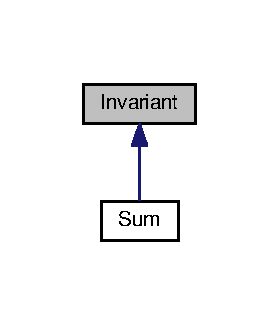
\includegraphics[width=134pt]{class_invariant__inherit__graph}
\end{center}
\end{figure}
\subsection*{Public Member Functions}
\begin{DoxyCompactItemize}
\item 
\hyperlink{class_invariant_aee61aac8e05fd3e6162b5b42655b4784}{Invariant} ()
\item 
\hyperlink{class_invariant_ac45b5d3cf54ef322c9827c603e4d1a56}{Invariant} (const \hyperlink{class_invariant}{Invariant} \&a)
\item 
virtual void \hyperlink{class_invariant_a76632dc09fe3537f159230620406fdff}{add\-Change} (int variable\-Number, int change)
\item 
virtual int \hyperlink{class_invariant_a4797e907bd38e68769962949b453ae7a}{calculate\-Delta\-Value} ()
\item 
virtual void \hyperlink{class_invariant_af04129a6e93870f87bc841db6475ae58}{initialize} ()
\item 
int \hyperlink{class_invariant_a4a5784dedbcafc641a927e47a5979b8f}{get\-Delta\-Value} ()
\item 
virtual bool \hyperlink{class_invariant_ab3fd6fa5c99ed9854756347a439e0fd9}{test} ()
\item 
virtual \hyperlink{class_invariant_a5e04ac8b0598cb050b485adebe0d5996}{$\sim$\-Invariant} ()
\item 
int \hyperlink{class_invariant_a570739630823019ab560dcf5ed5d9c79}{get\-Current\-Value} ()
\item 
void \hyperlink{class_invariant_ad6a0db294da40ee07bc432e4c082bdcd}{update\-Value} ()
\item 
void \hyperlink{class_invariant_a8c29176c35253050aabc33f43242c5b2}{set\-Used\-By\-Constraint} (int \hyperlink{_constants_8hpp_ab3a9f5ca3242dd173f530bb9f68fc611}{constraint}, int priority)
\item 
void \hyperlink{class_invariant_a5f3ca0104c32cbbf6b1f943b4691cc57}{set\-Used\-By\-Objective} (int objective)
\item 
int \hyperlink{class_invariant_aa8c83f6b8d3d1d907345d2784a7119ca}{get\-Constraint\-Number} ()
\item 
int \hyperlink{class_invariant_a77206bbdf0e95ac679787c18340c8ed7}{get\-Used\-In\-Objective} ()
\item 
unsigned \hyperlink{class_invariant_afff1e871c21c07ec683cced1733b9526}{get\-Priority} ()
\item 
int \hyperlink{class_invariant_a8b00f5d2bd3b5d656204ac3a3f051255}{get\-Type} ()
\item 
\hyperlink{_constants_8hpp_a5ea9d0c2efe357d2a7f5bcd80cdf179a}{Invariant\-Container} \& \hyperlink{class_invariant_a8bafd08ffb19446230d2c53ac5694e83}{get\-Update\-Vector} ()
\item 
void \hyperlink{class_invariant_af74c12c8720d388fc0897587d1c1d91c}{add\-To\-Update} (\hyperlink{_constants_8hpp_ac9b562f250a09412c017b68185321eba}{invariant} invar)
\item 
std\-::vector$<$ \hyperlink{class_integer_variable}{Integer\-Variable} $\ast$ $>$ \& \hyperlink{class_invariant_a09053cbce110bc98986bab0cbf03f322}{get\-Variables} ()
\item 
std\-::unordered\-\_\-map$<$ int, \hyperlink{_constants_8hpp_a08c47c54ab9fb1545c341ec853cc2278}{coef\-Type} $>$ \hyperlink{class_invariant_a35361b85223cf640130f903b795e7d9f}{get\-Coefficients} ()
\begin{DoxyCompactList}\small\item\em Passing by value. \end{DoxyCompactList}\item 
int \hyperlink{class_invariant_adc8d7a742f61131108e8be28fc7b7398}{get\-Variable\-I\-D} ()
\begin{DoxyCompactList}\small\item\em Only used when the invariant defines a variable through a oneway constraint. \end{DoxyCompactList}\end{DoxyCompactItemize}
\subsection*{Protected Attributes}
\begin{DoxyCompactItemize}
\item 
std\-::vector$<$ \hyperlink{class_integer_variable}{Integer\-Variable} $\ast$ $>$ \hyperlink{class_invariant_a86da68637f1714836eb31c302c01362b}{Variable\-Pointers}
\begin{DoxyCompactList}\small\item\em Correspond to the priority the invariant should be updated. \end{DoxyCompactList}\item 
double \hyperlink{class_invariant_a7208e25abfb820cc51b10659316deef2}{Current\-Value} = 0
\item 
double \hyperlink{class_invariant_ad447ae680438882a5c7fdd413ac3f672}{Delta\-Value} = 0
\item 
unsigned \hyperlink{class_invariant_a8d6f849b13550302c1d8e6f864f3962d}{constraint\-Priority}
\item 
int \hyperlink{class_invariant_a504c74e6a18a4e5bc2725961973d0fb3}{used\-In\-Constraint\-Nr}
\item 
int \hyperlink{class_invariant_a938a068c1f8bf551a2f53fba703927b1}{used\-In\-Objective\-Nr}
\item 
std\-::unordered\-\_\-map$<$ int, \hyperlink{_constants_8hpp_a08c47c54ab9fb1545c341ec853cc2278}{coef\-Type} $>$ \hyperlink{class_invariant_a6967f2c1b39c944ffd432528c40d4f23}{coefficients}
\item 
int \hyperlink{class_invariant_ae3f0977038deba2ace1016bc08c35c16}{type}
\item 
int \hyperlink{class_invariant_a7ec1254b39fa2214a2651e366d7dd4b1}{start\-Value} = 0
\begin{DoxyCompactList}\small\item\em Should be defined when creating oneway constraints that define (integer)variables. \end{DoxyCompactList}\item 
int \hyperlink{class_invariant_a7fe4c133c9815c49a3fa4e1ff38b444a}{variable\-I\-D}
\item 
\hyperlink{_constants_8hpp_a5ea9d0c2efe357d2a7f5bcd80cdf179a}{Invariant\-Container} \hyperlink{class_invariant_aca92a5d3c48153074a3b542ed7d8bb88}{invariants}
\item 
\hyperlink{_constants_8hpp_a5ea9d0c2efe357d2a7f5bcd80cdf179a}{Invariant\-Container} \hyperlink{class_invariant_ac88f162ea49e7b4469917e010f639da3}{update}
\end{DoxyCompactItemize}
\subsection*{Friends}
\begin{DoxyCompactItemize}
\item 
class \hyperlink{class_invariant_a831d0dd732f452551b0c77214ccbf558}{General\-Solver}
\end{DoxyCompactItemize}


\subsection{Constructor \& Destructor Documentation}
\hypertarget{class_invariant_aee61aac8e05fd3e6162b5b42655b4784}{\index{Invariant@{Invariant}!Invariant@{Invariant}}
\index{Invariant@{Invariant}!Invariant@{Invariant}}
\subsubsection[{Invariant}]{\setlength{\rightskip}{0pt plus 5cm}Invariant\-::\-Invariant (
\begin{DoxyParamCaption}
{}
\end{DoxyParamCaption}
)\hspace{0.3cm}{\ttfamily [inline]}}}\label{class_invariant_aee61aac8e05fd3e6162b5b42655b4784}
\hypertarget{class_invariant_ac45b5d3cf54ef322c9827c603e4d1a56}{\index{Invariant@{Invariant}!Invariant@{Invariant}}
\index{Invariant@{Invariant}!Invariant@{Invariant}}
\subsubsection[{Invariant}]{\setlength{\rightskip}{0pt plus 5cm}Invariant\-::\-Invariant (
\begin{DoxyParamCaption}
\item[{const {\bf Invariant} \&}]{a}
\end{DoxyParamCaption}
)\hspace{0.3cm}{\ttfamily [inline]}}}\label{class_invariant_ac45b5d3cf54ef322c9827c603e4d1a56}
\hypertarget{class_invariant_a5e04ac8b0598cb050b485adebe0d5996}{\index{Invariant@{Invariant}!$\sim$\-Invariant@{$\sim$\-Invariant}}
\index{$\sim$\-Invariant@{$\sim$\-Invariant}!Invariant@{Invariant}}
\subsubsection[{$\sim$\-Invariant}]{\setlength{\rightskip}{0pt plus 5cm}virtual Invariant\-::$\sim$\-Invariant (
\begin{DoxyParamCaption}
{}
\end{DoxyParamCaption}
)\hspace{0.3cm}{\ttfamily [inline]}, {\ttfamily [virtual]}}}\label{class_invariant_a5e04ac8b0598cb050b485adebe0d5996}


\subsection{Member Function Documentation}
\hypertarget{class_invariant_a76632dc09fe3537f159230620406fdff}{\index{Invariant@{Invariant}!add\-Change@{add\-Change}}
\index{add\-Change@{add\-Change}!Invariant@{Invariant}}
\subsubsection[{add\-Change}]{\setlength{\rightskip}{0pt plus 5cm}virtual void Invariant\-::add\-Change (
\begin{DoxyParamCaption}
\item[{int}]{variable\-Number, }
\item[{int}]{change}
\end{DoxyParamCaption}
)\hspace{0.3cm}{\ttfamily [inline]}, {\ttfamily [virtual]}}}\label{class_invariant_a76632dc09fe3537f159230620406fdff}


Reimplemented in \hyperlink{class_sum_aa66687e018c67ebedcabd69750374e2d}{Sum}.

\hypertarget{class_invariant_af74c12c8720d388fc0897587d1c1d91c}{\index{Invariant@{Invariant}!add\-To\-Update@{add\-To\-Update}}
\index{add\-To\-Update@{add\-To\-Update}!Invariant@{Invariant}}
\subsubsection[{add\-To\-Update}]{\setlength{\rightskip}{0pt plus 5cm}void Invariant\-::add\-To\-Update (
\begin{DoxyParamCaption}
\item[{{\bf invariant}}]{invar}
\end{DoxyParamCaption}
)\hspace{0.3cm}{\ttfamily [inline]}}}\label{class_invariant_af74c12c8720d388fc0897587d1c1d91c}
\hypertarget{class_invariant_a4797e907bd38e68769962949b453ae7a}{\index{Invariant@{Invariant}!calculate\-Delta\-Value@{calculate\-Delta\-Value}}
\index{calculate\-Delta\-Value@{calculate\-Delta\-Value}!Invariant@{Invariant}}
\subsubsection[{calculate\-Delta\-Value}]{\setlength{\rightskip}{0pt plus 5cm}virtual int Invariant\-::calculate\-Delta\-Value (
\begin{DoxyParamCaption}
{}
\end{DoxyParamCaption}
)\hspace{0.3cm}{\ttfamily [inline]}, {\ttfamily [virtual]}}}\label{class_invariant_a4797e907bd38e68769962949b453ae7a}


Reimplemented in \hyperlink{class_sum_a6b0ada7dc577609e3140a8695155f280}{Sum}.

\hypertarget{class_invariant_a35361b85223cf640130f903b795e7d9f}{\index{Invariant@{Invariant}!get\-Coefficients@{get\-Coefficients}}
\index{get\-Coefficients@{get\-Coefficients}!Invariant@{Invariant}}
\subsubsection[{get\-Coefficients}]{\setlength{\rightskip}{0pt plus 5cm}std\-::unordered\-\_\-map$<$int, {\bf coef\-Type}$>$ Invariant\-::get\-Coefficients (
\begin{DoxyParamCaption}
{}
\end{DoxyParamCaption}
)\hspace{0.3cm}{\ttfamily [inline]}}}\label{class_invariant_a35361b85223cf640130f903b795e7d9f}


Passing by value. 

\hypertarget{class_invariant_aa8c83f6b8d3d1d907345d2784a7119ca}{\index{Invariant@{Invariant}!get\-Constraint\-Number@{get\-Constraint\-Number}}
\index{get\-Constraint\-Number@{get\-Constraint\-Number}!Invariant@{Invariant}}
\subsubsection[{get\-Constraint\-Number}]{\setlength{\rightskip}{0pt plus 5cm}int Invariant\-::get\-Constraint\-Number (
\begin{DoxyParamCaption}
{}
\end{DoxyParamCaption}
)\hspace{0.3cm}{\ttfamily [inline]}}}\label{class_invariant_aa8c83f6b8d3d1d907345d2784a7119ca}
\hypertarget{class_invariant_a570739630823019ab560dcf5ed5d9c79}{\index{Invariant@{Invariant}!get\-Current\-Value@{get\-Current\-Value}}
\index{get\-Current\-Value@{get\-Current\-Value}!Invariant@{Invariant}}
\subsubsection[{get\-Current\-Value}]{\setlength{\rightskip}{0pt plus 5cm}int Invariant\-::get\-Current\-Value (
\begin{DoxyParamCaption}
{}
\end{DoxyParamCaption}
)\hspace{0.3cm}{\ttfamily [inline]}}}\label{class_invariant_a570739630823019ab560dcf5ed5d9c79}
\hypertarget{class_invariant_a4a5784dedbcafc641a927e47a5979b8f}{\index{Invariant@{Invariant}!get\-Delta\-Value@{get\-Delta\-Value}}
\index{get\-Delta\-Value@{get\-Delta\-Value}!Invariant@{Invariant}}
\subsubsection[{get\-Delta\-Value}]{\setlength{\rightskip}{0pt plus 5cm}int Invariant\-::get\-Delta\-Value (
\begin{DoxyParamCaption}
{}
\end{DoxyParamCaption}
)\hspace{0.3cm}{\ttfamily [inline]}}}\label{class_invariant_a4a5784dedbcafc641a927e47a5979b8f}
\hypertarget{class_invariant_afff1e871c21c07ec683cced1733b9526}{\index{Invariant@{Invariant}!get\-Priority@{get\-Priority}}
\index{get\-Priority@{get\-Priority}!Invariant@{Invariant}}
\subsubsection[{get\-Priority}]{\setlength{\rightskip}{0pt plus 5cm}unsigned Invariant\-::get\-Priority (
\begin{DoxyParamCaption}
{}
\end{DoxyParamCaption}
)\hspace{0.3cm}{\ttfamily [inline]}}}\label{class_invariant_afff1e871c21c07ec683cced1733b9526}
\hypertarget{class_invariant_a8b00f5d2bd3b5d656204ac3a3f051255}{\index{Invariant@{Invariant}!get\-Type@{get\-Type}}
\index{get\-Type@{get\-Type}!Invariant@{Invariant}}
\subsubsection[{get\-Type}]{\setlength{\rightskip}{0pt plus 5cm}int Invariant\-::get\-Type (
\begin{DoxyParamCaption}
{}
\end{DoxyParamCaption}
)\hspace{0.3cm}{\ttfamily [inline]}}}\label{class_invariant_a8b00f5d2bd3b5d656204ac3a3f051255}
\hypertarget{class_invariant_a8bafd08ffb19446230d2c53ac5694e83}{\index{Invariant@{Invariant}!get\-Update\-Vector@{get\-Update\-Vector}}
\index{get\-Update\-Vector@{get\-Update\-Vector}!Invariant@{Invariant}}
\subsubsection[{get\-Update\-Vector}]{\setlength{\rightskip}{0pt plus 5cm}{\bf Invariant\-Container}\& Invariant\-::get\-Update\-Vector (
\begin{DoxyParamCaption}
{}
\end{DoxyParamCaption}
)\hspace{0.3cm}{\ttfamily [inline]}}}\label{class_invariant_a8bafd08ffb19446230d2c53ac5694e83}
\hypertarget{class_invariant_a77206bbdf0e95ac679787c18340c8ed7}{\index{Invariant@{Invariant}!get\-Used\-In\-Objective@{get\-Used\-In\-Objective}}
\index{get\-Used\-In\-Objective@{get\-Used\-In\-Objective}!Invariant@{Invariant}}
\subsubsection[{get\-Used\-In\-Objective}]{\setlength{\rightskip}{0pt plus 5cm}int Invariant\-::get\-Used\-In\-Objective (
\begin{DoxyParamCaption}
{}
\end{DoxyParamCaption}
)\hspace{0.3cm}{\ttfamily [inline]}}}\label{class_invariant_a77206bbdf0e95ac679787c18340c8ed7}
\hypertarget{class_invariant_adc8d7a742f61131108e8be28fc7b7398}{\index{Invariant@{Invariant}!get\-Variable\-I\-D@{get\-Variable\-I\-D}}
\index{get\-Variable\-I\-D@{get\-Variable\-I\-D}!Invariant@{Invariant}}
\subsubsection[{get\-Variable\-I\-D}]{\setlength{\rightskip}{0pt plus 5cm}int Invariant\-::get\-Variable\-I\-D (
\begin{DoxyParamCaption}
{}
\end{DoxyParamCaption}
)\hspace{0.3cm}{\ttfamily [inline]}}}\label{class_invariant_adc8d7a742f61131108e8be28fc7b7398}


Only used when the invariant defines a variable through a oneway constraint. 

\hypertarget{class_invariant_a09053cbce110bc98986bab0cbf03f322}{\index{Invariant@{Invariant}!get\-Variables@{get\-Variables}}
\index{get\-Variables@{get\-Variables}!Invariant@{Invariant}}
\subsubsection[{get\-Variables}]{\setlength{\rightskip}{0pt plus 5cm}std\-::vector$<${\bf Integer\-Variable}$\ast$$>$\& Invariant\-::get\-Variables (
\begin{DoxyParamCaption}
{}
\end{DoxyParamCaption}
)\hspace{0.3cm}{\ttfamily [inline]}}}\label{class_invariant_a09053cbce110bc98986bab0cbf03f322}
\hypertarget{class_invariant_af04129a6e93870f87bc841db6475ae58}{\index{Invariant@{Invariant}!initialize@{initialize}}
\index{initialize@{initialize}!Invariant@{Invariant}}
\subsubsection[{initialize}]{\setlength{\rightskip}{0pt plus 5cm}virtual void Invariant\-::initialize (
\begin{DoxyParamCaption}
{}
\end{DoxyParamCaption}
)\hspace{0.3cm}{\ttfamily [inline]}, {\ttfamily [virtual]}}}\label{class_invariant_af04129a6e93870f87bc841db6475ae58}
\hypertarget{class_invariant_a8c29176c35253050aabc33f43242c5b2}{\index{Invariant@{Invariant}!set\-Used\-By\-Constraint@{set\-Used\-By\-Constraint}}
\index{set\-Used\-By\-Constraint@{set\-Used\-By\-Constraint}!Invariant@{Invariant}}
\subsubsection[{set\-Used\-By\-Constraint}]{\setlength{\rightskip}{0pt plus 5cm}void Invariant\-::set\-Used\-By\-Constraint (
\begin{DoxyParamCaption}
\item[{int}]{constraint, }
\item[{int}]{priority}
\end{DoxyParamCaption}
)\hspace{0.3cm}{\ttfamily [inline]}}}\label{class_invariant_a8c29176c35253050aabc33f43242c5b2}
\hypertarget{class_invariant_a5f3ca0104c32cbbf6b1f943b4691cc57}{\index{Invariant@{Invariant}!set\-Used\-By\-Objective@{set\-Used\-By\-Objective}}
\index{set\-Used\-By\-Objective@{set\-Used\-By\-Objective}!Invariant@{Invariant}}
\subsubsection[{set\-Used\-By\-Objective}]{\setlength{\rightskip}{0pt plus 5cm}void Invariant\-::set\-Used\-By\-Objective (
\begin{DoxyParamCaption}
\item[{int}]{objective}
\end{DoxyParamCaption}
)\hspace{0.3cm}{\ttfamily [inline]}}}\label{class_invariant_a5f3ca0104c32cbbf6b1f943b4691cc57}
\hypertarget{class_invariant_ab3fd6fa5c99ed9854756347a439e0fd9}{\index{Invariant@{Invariant}!test@{test}}
\index{test@{test}!Invariant@{Invariant}}
\subsubsection[{test}]{\setlength{\rightskip}{0pt plus 5cm}virtual bool Invariant\-::test (
\begin{DoxyParamCaption}
{}
\end{DoxyParamCaption}
)\hspace{0.3cm}{\ttfamily [inline]}, {\ttfamily [virtual]}}}\label{class_invariant_ab3fd6fa5c99ed9854756347a439e0fd9}


Reimplemented in \hyperlink{class_sum_a1adcbbefeb5f25445563fada563d4fa1}{Sum}.

\hypertarget{class_invariant_ad6a0db294da40ee07bc432e4c082bdcd}{\index{Invariant@{Invariant}!update\-Value@{update\-Value}}
\index{update\-Value@{update\-Value}!Invariant@{Invariant}}
\subsubsection[{update\-Value}]{\setlength{\rightskip}{0pt plus 5cm}void Invariant\-::update\-Value (
\begin{DoxyParamCaption}
{}
\end{DoxyParamCaption}
)\hspace{0.3cm}{\ttfamily [inline]}}}\label{class_invariant_ad6a0db294da40ee07bc432e4c082bdcd}


\subsection{Friends And Related Function Documentation}
\hypertarget{class_invariant_a831d0dd732f452551b0c77214ccbf558}{\index{Invariant@{Invariant}!General\-Solver@{General\-Solver}}
\index{General\-Solver@{General\-Solver}!Invariant@{Invariant}}
\subsubsection[{General\-Solver}]{\setlength{\rightskip}{0pt plus 5cm}friend class {\bf General\-Solver}\hspace{0.3cm}{\ttfamily [friend]}}}\label{class_invariant_a831d0dd732f452551b0c77214ccbf558}


\subsection{Member Data Documentation}
\hypertarget{class_invariant_a6967f2c1b39c944ffd432528c40d4f23}{\index{Invariant@{Invariant}!coefficients@{coefficients}}
\index{coefficients@{coefficients}!Invariant@{Invariant}}
\subsubsection[{coefficients}]{\setlength{\rightskip}{0pt plus 5cm}std\-::unordered\-\_\-map$<$int, {\bf coef\-Type}$>$ Invariant\-::coefficients\hspace{0.3cm}{\ttfamily [protected]}}}\label{class_invariant_a6967f2c1b39c944ffd432528c40d4f23}
\hypertarget{class_invariant_a8d6f849b13550302c1d8e6f864f3962d}{\index{Invariant@{Invariant}!constraint\-Priority@{constraint\-Priority}}
\index{constraint\-Priority@{constraint\-Priority}!Invariant@{Invariant}}
\subsubsection[{constraint\-Priority}]{\setlength{\rightskip}{0pt plus 5cm}unsigned Invariant\-::constraint\-Priority\hspace{0.3cm}{\ttfamily [protected]}}}\label{class_invariant_a8d6f849b13550302c1d8e6f864f3962d}
\hypertarget{class_invariant_a7208e25abfb820cc51b10659316deef2}{\index{Invariant@{Invariant}!Current\-Value@{Current\-Value}}
\index{Current\-Value@{Current\-Value}!Invariant@{Invariant}}
\subsubsection[{Current\-Value}]{\setlength{\rightskip}{0pt plus 5cm}double Invariant\-::\-Current\-Value = 0\hspace{0.3cm}{\ttfamily [protected]}}}\label{class_invariant_a7208e25abfb820cc51b10659316deef2}
\hypertarget{class_invariant_ad447ae680438882a5c7fdd413ac3f672}{\index{Invariant@{Invariant}!Delta\-Value@{Delta\-Value}}
\index{Delta\-Value@{Delta\-Value}!Invariant@{Invariant}}
\subsubsection[{Delta\-Value}]{\setlength{\rightskip}{0pt plus 5cm}double Invariant\-::\-Delta\-Value = 0\hspace{0.3cm}{\ttfamily [protected]}}}\label{class_invariant_ad447ae680438882a5c7fdd413ac3f672}
\hypertarget{class_invariant_aca92a5d3c48153074a3b542ed7d8bb88}{\index{Invariant@{Invariant}!invariants@{invariants}}
\index{invariants@{invariants}!Invariant@{Invariant}}
\subsubsection[{invariants}]{\setlength{\rightskip}{0pt plus 5cm}{\bf Invariant\-Container} Invariant\-::invariants\hspace{0.3cm}{\ttfamily [protected]}}}\label{class_invariant_aca92a5d3c48153074a3b542ed7d8bb88}
\hypertarget{class_invariant_a7ec1254b39fa2214a2651e366d7dd4b1}{\index{Invariant@{Invariant}!start\-Value@{start\-Value}}
\index{start\-Value@{start\-Value}!Invariant@{Invariant}}
\subsubsection[{start\-Value}]{\setlength{\rightskip}{0pt plus 5cm}int Invariant\-::start\-Value = 0\hspace{0.3cm}{\ttfamily [protected]}}}\label{class_invariant_a7ec1254b39fa2214a2651e366d7dd4b1}


Should be defined when creating oneway constraints that define (integer)variables. 

\hypertarget{class_invariant_ae3f0977038deba2ace1016bc08c35c16}{\index{Invariant@{Invariant}!type@{type}}
\index{type@{type}!Invariant@{Invariant}}
\subsubsection[{type}]{\setlength{\rightskip}{0pt plus 5cm}int Invariant\-::type\hspace{0.3cm}{\ttfamily [protected]}}}\label{class_invariant_ae3f0977038deba2ace1016bc08c35c16}
\hypertarget{class_invariant_ac88f162ea49e7b4469917e010f639da3}{\index{Invariant@{Invariant}!update@{update}}
\index{update@{update}!Invariant@{Invariant}}
\subsubsection[{update}]{\setlength{\rightskip}{0pt plus 5cm}{\bf Invariant\-Container} Invariant\-::update\hspace{0.3cm}{\ttfamily [protected]}}}\label{class_invariant_ac88f162ea49e7b4469917e010f639da3}
\hypertarget{class_invariant_a504c74e6a18a4e5bc2725961973d0fb3}{\index{Invariant@{Invariant}!used\-In\-Constraint\-Nr@{used\-In\-Constraint\-Nr}}
\index{used\-In\-Constraint\-Nr@{used\-In\-Constraint\-Nr}!Invariant@{Invariant}}
\subsubsection[{used\-In\-Constraint\-Nr}]{\setlength{\rightskip}{0pt plus 5cm}int Invariant\-::used\-In\-Constraint\-Nr\hspace{0.3cm}{\ttfamily [protected]}}}\label{class_invariant_a504c74e6a18a4e5bc2725961973d0fb3}
\hypertarget{class_invariant_a938a068c1f8bf551a2f53fba703927b1}{\index{Invariant@{Invariant}!used\-In\-Objective\-Nr@{used\-In\-Objective\-Nr}}
\index{used\-In\-Objective\-Nr@{used\-In\-Objective\-Nr}!Invariant@{Invariant}}
\subsubsection[{used\-In\-Objective\-Nr}]{\setlength{\rightskip}{0pt plus 5cm}int Invariant\-::used\-In\-Objective\-Nr\hspace{0.3cm}{\ttfamily [protected]}}}\label{class_invariant_a938a068c1f8bf551a2f53fba703927b1}
\hypertarget{class_invariant_a7fe4c133c9815c49a3fa4e1ff38b444a}{\index{Invariant@{Invariant}!variable\-I\-D@{variable\-I\-D}}
\index{variable\-I\-D@{variable\-I\-D}!Invariant@{Invariant}}
\subsubsection[{variable\-I\-D}]{\setlength{\rightskip}{0pt plus 5cm}int Invariant\-::variable\-I\-D\hspace{0.3cm}{\ttfamily [protected]}}}\label{class_invariant_a7fe4c133c9815c49a3fa4e1ff38b444a}
\hypertarget{class_invariant_a86da68637f1714836eb31c302c01362b}{\index{Invariant@{Invariant}!Variable\-Pointers@{Variable\-Pointers}}
\index{Variable\-Pointers@{Variable\-Pointers}!Invariant@{Invariant}}
\subsubsection[{Variable\-Pointers}]{\setlength{\rightskip}{0pt plus 5cm}std\-::vector$<${\bf Integer\-Variable}$\ast$$>$ Invariant\-::\-Variable\-Pointers\hspace{0.3cm}{\ttfamily [protected]}}}\label{class_invariant_a86da68637f1714836eb31c302c01362b}


Correspond to the priority the invariant should be updated. 



The documentation for this class was generated from the following file\-:\begin{DoxyCompactItemize}
\item 
\hyperlink{_invariant_8hpp}{Invariant.\-hpp}\end{DoxyCompactItemize}

\hypertarget{class_linear}{\section{Linear Class Reference}
\label{class_linear}\index{Linear@{Linear}}
}


{\ttfamily \#include $<$Linear.\-hpp$>$}



Inheritance diagram for Linear\-:\nopagebreak
\begin{figure}[H]
\begin{center}
\leavevmode
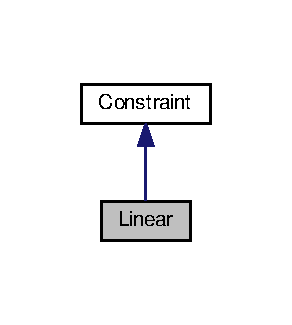
\includegraphics[width=140pt]{class_linear__inherit__graph}
\end{center}
\end{figure}


Collaboration diagram for Linear\-:\nopagebreak
\begin{figure}[H]
\begin{center}
\leavevmode
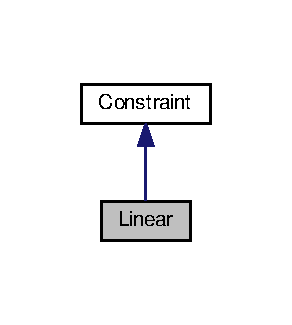
\includegraphics[width=140pt]{class_linear__coll__graph}
\end{center}
\end{figure}
\subsection*{Public Member Functions}
\begin{DoxyCompactItemize}
\item 
\hyperlink{class_linear_a4e7a378e3e338a36505d0ac001f46f16}{Linear} (std\-::vector$<$ int $>$ \&\hyperlink{class_constraint_a976da5d8a1e74efb119f47094b721df9}{coefficients}, std\-::vector$<$ \hyperlink{class_integer_variable}{Integer\-Variable} $\ast$ $>$ \&\hyperlink{class_constraint_abd73767b8640c514f582a9316a1ce792}{variables}, int ub, int \hyperlink{class_linear_a0c01f7a40f3e0ed8d6466058da3c2e09}{relation})
\begin{DoxyCompactList}\small\item\em Used to create the original (given by user) constraints. \end{DoxyCompactList}\item 
\hyperlink{class_linear_a6abe6c2b55a1e1c3e838aaf82e77e627}{$\sim$\-Linear} ()
\begin{DoxyCompactList}\small\item\em Used to create the \hyperlink{class_linear}{Linear} constraint used by local search. \end{DoxyCompactList}\item 
int \hyperlink{class_linear_aedc905d17bf15995d165e2a4be4c4bd7}{set\-Delta\-Violation} ()
\item 
int \hyperlink{class_linear_a18a38d26f82871299834fbf7b5fdfbf2}{set\-Delta\-Violation\-Degree} ()
\item 
int \hyperlink{class_linear_ae51920a533c6b8e86e07b1c1d37c05fd}{update\-Violation} ()
\item 
int \hyperlink{class_linear_a21831311c105f308c01fa371a2f8fec7}{update\-Violation\-Degree} ()
\item 
bool \hyperlink{class_linear_af8bb974adb2e4d510f325d4865dc5272}{test\-Cons} ()
\item 
bool \hyperlink{class_linear_a84cb459a43191d04406b756117ff8eef}{test\-Obj} ()
\end{DoxyCompactItemize}
\subsection*{Protected Attributes}
\begin{DoxyCompactItemize}
\item 
int \hyperlink{class_linear_a1c5f6c022a68b273fadc1d16f0c431b0}{rhs}
\item 
int \hyperlink{class_linear_a0c01f7a40f3e0ed8d6466058da3c2e09}{relation}
\end{DoxyCompactItemize}


\subsection{Constructor \& Destructor Documentation}
\hypertarget{class_linear_a4e7a378e3e338a36505d0ac001f46f16}{\index{Linear@{Linear}!Linear@{Linear}}
\index{Linear@{Linear}!Linear@{Linear}}
\subsubsection[{Linear}]{\setlength{\rightskip}{0pt plus 5cm}Linear\-::\-Linear (
\begin{DoxyParamCaption}
\item[{std\-::vector$<$ int $>$ \&}]{coefficients, }
\item[{std\-::vector$<$ {\bf Integer\-Variable} $\ast$ $>$ \&}]{variables, }
\item[{int}]{ub, }
\item[{int}]{relation}
\end{DoxyParamCaption}
)\hspace{0.3cm}{\ttfamily [inline]}}}\label{class_linear_a4e7a378e3e338a36505d0ac001f46f16}


Used to create the original (given by user) constraints. 

\hypertarget{class_linear_a6abe6c2b55a1e1c3e838aaf82e77e627}{\index{Linear@{Linear}!$\sim$\-Linear@{$\sim$\-Linear}}
\index{$\sim$\-Linear@{$\sim$\-Linear}!Linear@{Linear}}
\subsubsection[{$\sim$\-Linear}]{\setlength{\rightskip}{0pt plus 5cm}Linear\-::$\sim$\-Linear (
\begin{DoxyParamCaption}
{}
\end{DoxyParamCaption}
)\hspace{0.3cm}{\ttfamily [inline]}}}\label{class_linear_a6abe6c2b55a1e1c3e838aaf82e77e627}


Used to create the \hyperlink{class_linear}{Linear} constraint used by local search. 



\subsection{Member Function Documentation}
\hypertarget{class_linear_aedc905d17bf15995d165e2a4be4c4bd7}{\index{Linear@{Linear}!set\-Delta\-Violation@{set\-Delta\-Violation}}
\index{set\-Delta\-Violation@{set\-Delta\-Violation}!Linear@{Linear}}
\subsubsection[{set\-Delta\-Violation}]{\setlength{\rightskip}{0pt plus 5cm}int Linear\-::set\-Delta\-Violation (
\begin{DoxyParamCaption}
{}
\end{DoxyParamCaption}
)\hspace{0.3cm}{\ttfamily [inline]}, {\ttfamily [virtual]}}}\label{class_linear_aedc905d17bf15995d165e2a4be4c4bd7}


Reimplemented from \hyperlink{class_constraint_a838ed3f4029d443c3193524be0c8f977}{Constraint}.

\hypertarget{class_linear_a18a38d26f82871299834fbf7b5fdfbf2}{\index{Linear@{Linear}!set\-Delta\-Violation\-Degree@{set\-Delta\-Violation\-Degree}}
\index{set\-Delta\-Violation\-Degree@{set\-Delta\-Violation\-Degree}!Linear@{Linear}}
\subsubsection[{set\-Delta\-Violation\-Degree}]{\setlength{\rightskip}{0pt plus 5cm}int Linear\-::set\-Delta\-Violation\-Degree (
\begin{DoxyParamCaption}
{}
\end{DoxyParamCaption}
)\hspace{0.3cm}{\ttfamily [inline]}, {\ttfamily [virtual]}}}\label{class_linear_a18a38d26f82871299834fbf7b5fdfbf2}


Reimplemented from \hyperlink{class_constraint_aaa22c193fec13cbdc29875a1a90f65d6}{Constraint}.

\hypertarget{class_linear_af8bb974adb2e4d510f325d4865dc5272}{\index{Linear@{Linear}!test\-Cons@{test\-Cons}}
\index{test\-Cons@{test\-Cons}!Linear@{Linear}}
\subsubsection[{test\-Cons}]{\setlength{\rightskip}{0pt plus 5cm}bool Linear\-::test\-Cons (
\begin{DoxyParamCaption}
{}
\end{DoxyParamCaption}
)\hspace{0.3cm}{\ttfamily [inline]}, {\ttfamily [virtual]}}}\label{class_linear_af8bb974adb2e4d510f325d4865dc5272}


Reimplemented from \hyperlink{class_constraint_affe33a000e4eedc012ae184617534225}{Constraint}.

\hypertarget{class_linear_a84cb459a43191d04406b756117ff8eef}{\index{Linear@{Linear}!test\-Obj@{test\-Obj}}
\index{test\-Obj@{test\-Obj}!Linear@{Linear}}
\subsubsection[{test\-Obj}]{\setlength{\rightskip}{0pt plus 5cm}bool Linear\-::test\-Obj (
\begin{DoxyParamCaption}
{}
\end{DoxyParamCaption}
)\hspace{0.3cm}{\ttfamily [inline]}, {\ttfamily [virtual]}}}\label{class_linear_a84cb459a43191d04406b756117ff8eef}


Reimplemented from \hyperlink{class_constraint_a564d47f24c7cdccf1c5a7b3fd91c0743}{Constraint}.

\hypertarget{class_linear_ae51920a533c6b8e86e07b1c1d37c05fd}{\index{Linear@{Linear}!update\-Violation@{update\-Violation}}
\index{update\-Violation@{update\-Violation}!Linear@{Linear}}
\subsubsection[{update\-Violation}]{\setlength{\rightskip}{0pt plus 5cm}int Linear\-::update\-Violation (
\begin{DoxyParamCaption}
{}
\end{DoxyParamCaption}
)\hspace{0.3cm}{\ttfamily [inline]}, {\ttfamily [virtual]}}}\label{class_linear_ae51920a533c6b8e86e07b1c1d37c05fd}


Reimplemented from \hyperlink{class_constraint_a3dbfd62667a4d7c06fdfbd0b38608fca}{Constraint}.

\hypertarget{class_linear_a21831311c105f308c01fa371a2f8fec7}{\index{Linear@{Linear}!update\-Violation\-Degree@{update\-Violation\-Degree}}
\index{update\-Violation\-Degree@{update\-Violation\-Degree}!Linear@{Linear}}
\subsubsection[{update\-Violation\-Degree}]{\setlength{\rightskip}{0pt plus 5cm}int Linear\-::update\-Violation\-Degree (
\begin{DoxyParamCaption}
{}
\end{DoxyParamCaption}
)\hspace{0.3cm}{\ttfamily [inline]}, {\ttfamily [virtual]}}}\label{class_linear_a21831311c105f308c01fa371a2f8fec7}


Reimplemented from \hyperlink{class_constraint_a389d341b518e22981d7e8e4b8a16f739}{Constraint}.



\subsection{Member Data Documentation}
\hypertarget{class_linear_a0c01f7a40f3e0ed8d6466058da3c2e09}{\index{Linear@{Linear}!relation@{relation}}
\index{relation@{relation}!Linear@{Linear}}
\subsubsection[{relation}]{\setlength{\rightskip}{0pt plus 5cm}int Linear\-::relation\hspace{0.3cm}{\ttfamily [protected]}}}\label{class_linear_a0c01f7a40f3e0ed8d6466058da3c2e09}
\hypertarget{class_linear_a1c5f6c022a68b273fadc1d16f0c431b0}{\index{Linear@{Linear}!rhs@{rhs}}
\index{rhs@{rhs}!Linear@{Linear}}
\subsubsection[{rhs}]{\setlength{\rightskip}{0pt plus 5cm}int Linear\-::rhs\hspace{0.3cm}{\ttfamily [protected]}}}\label{class_linear_a1c5f6c022a68b273fadc1d16f0c431b0}


The documentation for this class was generated from the following file\-:\begin{DoxyCompactItemize}
\item 
\hyperlink{_linear_8hpp}{Linear.\-hpp}\end{DoxyCompactItemize}

\hypertarget{class_l_s_space}{\section{L\-S\-Space Class Reference}
\label{class_l_s_space}\index{L\-S\-Space@{L\-S\-Space}}
}


{\ttfamily \#include $<$L\-S\-Space.\-hpp$>$}

\subsection*{Public Member Functions}
\begin{DoxyCompactItemize}
\item 
\hyperlink{class_l_s_space_aece02fa05f80f4714dc001c1a0ecb641}{L\-S\-Space} (std\-::shared\-\_\-ptr$<$ \hyperlink{class_model}{Model} $>$ \hyperlink{class_l_s_space_a3d1e22bec1da147a2ef457ead60d7d4f}{model})
\item 
void \hyperlink{class_l_s_space_a2b850707c65dd649a2bd97339190f9c5}{print\-Current} ()
\item 
\hyperlink{class_l_s_space_ad7f43b3e335d28922aa74a497e278386}{$\sim$\-L\-S\-Space} ()
\item 
void \hyperlink{class_l_s_space_a0560c7a6614859e8986da97860138db7}{optimize\-Solution} (int time, std\-::shared\-\_\-ptr$<$ \hyperlink{class_state}{State} $>$ st)
\item 
void \hyperlink{class_l_s_space_ac1fe2858bf40a20f80dcc5511ac96751}{simple\-Move} (int variabel\-Nr)
\item 
bool \hyperlink{class_l_s_space_ad84c52c66de00faa45dda05a88cdd040}{best\-Improvement} ()
\end{DoxyCompactItemize}
\subsection*{Private Attributes}
\begin{DoxyCompactItemize}
\item 
int \hyperlink{class_l_s_space_a6f9048fcca7d13ce4394154af5ba0ed2}{Violations} = 0
\item 
int \hyperlink{class_l_s_space_acfd6b86c42c63f43a29bee6853a2992e}{iterations} = 0
\item 
std\-::shared\-\_\-ptr$<$ \hyperlink{class_model}{Model} $>$ \hyperlink{class_l_s_space_a3d1e22bec1da147a2ef457ead60d7d4f}{model}
\end{DoxyCompactItemize}
\subsection*{Friends}
\begin{DoxyCompactItemize}
\item 
class \hyperlink{class_l_s_space_a5b78b1c2e1fa07ffed92da365593eaa4}{Test}
\end{DoxyCompactItemize}


\subsection{Constructor \& Destructor Documentation}
\hypertarget{class_l_s_space_aece02fa05f80f4714dc001c1a0ecb641}{\index{L\-S\-Space@{L\-S\-Space}!L\-S\-Space@{L\-S\-Space}}
\index{L\-S\-Space@{L\-S\-Space}!LSSpace@{L\-S\-Space}}
\subsubsection[{L\-S\-Space}]{\setlength{\rightskip}{0pt plus 5cm}L\-S\-Space\-::\-L\-S\-Space (
\begin{DoxyParamCaption}
\item[{std\-::shared\-\_\-ptr$<$ {\bf Model} $>$}]{model}
\end{DoxyParamCaption}
)}}\label{class_l_s_space_aece02fa05f80f4714dc001c1a0ecb641}
\hypertarget{class_l_s_space_ad7f43b3e335d28922aa74a497e278386}{\index{L\-S\-Space@{L\-S\-Space}!$\sim$\-L\-S\-Space@{$\sim$\-L\-S\-Space}}
\index{$\sim$\-L\-S\-Space@{$\sim$\-L\-S\-Space}!LSSpace@{L\-S\-Space}}
\subsubsection[{$\sim$\-L\-S\-Space}]{\setlength{\rightskip}{0pt plus 5cm}L\-S\-Space\-::$\sim$\-L\-S\-Space (
\begin{DoxyParamCaption}
{}
\end{DoxyParamCaption}
)\hspace{0.3cm}{\ttfamily [inline]}}}\label{class_l_s_space_ad7f43b3e335d28922aa74a497e278386}


\subsection{Member Function Documentation}
\hypertarget{class_l_s_space_ad84c52c66de00faa45dda05a88cdd040}{\index{L\-S\-Space@{L\-S\-Space}!best\-Improvement@{best\-Improvement}}
\index{best\-Improvement@{best\-Improvement}!LSSpace@{L\-S\-Space}}
\subsubsection[{best\-Improvement}]{\setlength{\rightskip}{0pt plus 5cm}bool L\-S\-Space\-::best\-Improvement (
\begin{DoxyParamCaption}
{}
\end{DoxyParamCaption}
)}}\label{class_l_s_space_ad84c52c66de00faa45dda05a88cdd040}
\hypertarget{class_l_s_space_a0560c7a6614859e8986da97860138db7}{\index{L\-S\-Space@{L\-S\-Space}!optimize\-Solution@{optimize\-Solution}}
\index{optimize\-Solution@{optimize\-Solution}!LSSpace@{L\-S\-Space}}
\subsubsection[{optimize\-Solution}]{\setlength{\rightskip}{0pt plus 5cm}void L\-S\-Space\-::optimize\-Solution (
\begin{DoxyParamCaption}
\item[{int}]{time, }
\item[{std\-::shared\-\_\-ptr$<$ {\bf State} $>$}]{st}
\end{DoxyParamCaption}
)}}\label{class_l_s_space_a0560c7a6614859e8986da97860138db7}
\hypertarget{class_l_s_space_a2b850707c65dd649a2bd97339190f9c5}{\index{L\-S\-Space@{L\-S\-Space}!print\-Current@{print\-Current}}
\index{print\-Current@{print\-Current}!LSSpace@{L\-S\-Space}}
\subsubsection[{print\-Current}]{\setlength{\rightskip}{0pt plus 5cm}void L\-S\-Space\-::print\-Current (
\begin{DoxyParamCaption}
{}
\end{DoxyParamCaption}
)}}\label{class_l_s_space_a2b850707c65dd649a2bd97339190f9c5}
\hypertarget{class_l_s_space_ac1fe2858bf40a20f80dcc5511ac96751}{\index{L\-S\-Space@{L\-S\-Space}!simple\-Move@{simple\-Move}}
\index{simple\-Move@{simple\-Move}!LSSpace@{L\-S\-Space}}
\subsubsection[{simple\-Move}]{\setlength{\rightskip}{0pt plus 5cm}void L\-S\-Space\-::simple\-Move (
\begin{DoxyParamCaption}
\item[{int}]{variabel\-Nr}
\end{DoxyParamCaption}
)}}\label{class_l_s_space_ac1fe2858bf40a20f80dcc5511ac96751}


\subsection{Friends And Related Function Documentation}
\hypertarget{class_l_s_space_a5b78b1c2e1fa07ffed92da365593eaa4}{\index{L\-S\-Space@{L\-S\-Space}!Test@{Test}}
\index{Test@{Test}!LSSpace@{L\-S\-Space}}
\subsubsection[{Test}]{\setlength{\rightskip}{0pt plus 5cm}friend class Test\hspace{0.3cm}{\ttfamily [friend]}}}\label{class_l_s_space_a5b78b1c2e1fa07ffed92da365593eaa4}


\subsection{Member Data Documentation}
\hypertarget{class_l_s_space_acfd6b86c42c63f43a29bee6853a2992e}{\index{L\-S\-Space@{L\-S\-Space}!iterations@{iterations}}
\index{iterations@{iterations}!LSSpace@{L\-S\-Space}}
\subsubsection[{iterations}]{\setlength{\rightskip}{0pt plus 5cm}int L\-S\-Space\-::iterations = 0\hspace{0.3cm}{\ttfamily [private]}}}\label{class_l_s_space_acfd6b86c42c63f43a29bee6853a2992e}
\hypertarget{class_l_s_space_a3d1e22bec1da147a2ef457ead60d7d4f}{\index{L\-S\-Space@{L\-S\-Space}!model@{model}}
\index{model@{model}!LSSpace@{L\-S\-Space}}
\subsubsection[{model}]{\setlength{\rightskip}{0pt plus 5cm}std\-::shared\-\_\-ptr$<${\bf Model}$>$ L\-S\-Space\-::model\hspace{0.3cm}{\ttfamily [private]}}}\label{class_l_s_space_a3d1e22bec1da147a2ef457ead60d7d4f}
\hypertarget{class_l_s_space_a6f9048fcca7d13ce4394154af5ba0ed2}{\index{L\-S\-Space@{L\-S\-Space}!Violations@{Violations}}
\index{Violations@{Violations}!LSSpace@{L\-S\-Space}}
\subsubsection[{Violations}]{\setlength{\rightskip}{0pt plus 5cm}int L\-S\-Space\-::\-Violations = 0\hspace{0.3cm}{\ttfamily [private]}}}\label{class_l_s_space_a6f9048fcca7d13ce4394154af5ba0ed2}


The documentation for this class was generated from the following files\-:\begin{DoxyCompactItemize}
\item 
\hyperlink{_l_s_space_8hpp}{L\-S\-Space.\-hpp}\item 
\hyperlink{_l_s_space_8cpp}{L\-S\-Space.\-cpp}\end{DoxyCompactItemize}

\hypertarget{class_model}{\section{Model Class Reference}
\label{class_model}\index{Model@{Model}}
}


{\ttfamily \#include $<$Model.\-hpp$>$}

\subsection*{Public Member Functions}
\begin{DoxyCompactItemize}
\item 
\hyperlink{class_model_ae3b375de5f6df4faf74a95d64748e048}{Model} ()
\item 
\hyperlink{class_model_afdedf278781f785abeecf5f450e43653}{Model} (const \hyperlink{class_model}{Model} \&orig)
\item 
\hyperlink{class_model_ad6ebd2062a0b823db841a0b88baac4c0}{$\sim$\-Model} ()
\item 
void \hyperlink{class_model_ab4a45c7798de6427e24d4d0116db2e70}{add\-Binary\-Variable} (int lb, int ub)
\item 
void \hyperlink{class_model_a7b8e21078dbcbb489f985bf13b03f76e}{add\-Integer\-Variable} (int lb, int ub)
\item 
\hyperlink{class_integer_variable}{Integer\-Variable} $\ast$ \hyperlink{class_model_a7ab387183363c4784c44b5bcf8132198}{get\-Mask\-At} (int i)
\item 
std\-::vector$<$ \hyperlink{class_integer_variable}{Integer\-Variable} $\ast$ $>$ \& \hyperlink{class_model_a62dcb95de0df2587cb82f1dcc469b443}{get\-Mask} ()
\item 
std\-::list$<$ \hyperlink{class_integer_variable}{Integer\-Variable} $\ast$ $>$ \& \hyperlink{class_model_aa4dbcf1abedc835ac9017c320fbd91be}{get\-Integer\-Variables} ()
\begin{DoxyCompactList}\small\item\em Returns all integer variables as a list. only used to make oneway constraints. \end{DoxyCompactList}\item 
\hyperlink{_constants_8hpp_a30d6ea0a65b32e8b74cc6126cea9852e}{variable\-Container} \& \hyperlink{class_model_a8416f0b4c7db6b2a5ff5edf4aa0bf3db}{get\-Non\-Fixed\-Binary\-Variables} ()
\item 
\hyperlink{_constants_8hpp_a30d6ea0a65b32e8b74cc6126cea9852e}{variable\-Container} \& \hyperlink{class_model_acdcb4f81370ca74c301faceae32cb466}{get\-All\-Variables} ()
\item 
\hyperlink{_constants_8hpp_a5ea9d0c2efe357d2a7f5bcd80cdf179a}{Invariant\-Container} \& \hyperlink{class_model_aabfc3eb2ef3c57060792e45684a951b3}{get\-Invariants} ()
\item 
\hyperlink{_constants_8hpp_a44699d451ee649f131b1b72451070aa0}{constraint\-Container} \hyperlink{class_model_a169afc5a4132e106a9909ebb158f1e97}{get\-Constraints\-With\-Priority} (int prio)
\item 
\hyperlink{_constants_8hpp_a9cd92c30962a3af393035610635972fa}{all\-Constraints} \& \hyperlink{class_model_a84692604aec562f826ecd797f7c9a53e}{get\-Constraints} ()
\item 
\hyperlink{_constants_8hpp_a44699d451ee649f131b1b72451070aa0}{constraint\-Container} \hyperlink{class_model_a3a02bd2477b425dffb18af15541ab08f}{get\-Objectives} ()
\item 
\hyperlink{class_integer_variable}{Integer\-Variable} $\ast$ \hyperlink{class_model_a319b03ca9238413b4120b8edb67099b4}{get\-Non\-Fixed\-Binary\-Variable} (int i)
\item 
void \hyperlink{class_model_aea595e2853bd86b738ef0908137c4a9f}{update\-Integer\-Variable} (int index, Gecode\-::\-Int\-Var \&variable)
\item 
void \hyperlink{class_model_a2f6cc1ee8ac991843a43c9fac4a7da7b}{non\-Fixed\-Variables} (std\-::vector$<$ \hyperlink{class_integer_variable}{Integer\-Variable} $\ast$ $>$ $\ast$non\-Fixed)
\end{DoxyCompactItemize}
\subsection*{Public Attributes}
\begin{DoxyCompactItemize}
\item 
int \hyperlink{class_model_a69256596942801e8a166dabaf9a31114}{initial\-Value}
\begin{DoxyCompactList}\small\item\em Should be moved to state. \end{DoxyCompactList}\end{DoxyCompactItemize}
\subsection*{Private Attributes}
\begin{DoxyCompactItemize}
\item 
\hyperlink{_constants_8hpp_a30d6ea0a65b32e8b74cc6126cea9852e}{variable\-Container} \hyperlink{class_model_ad313212f7d87f5b57c0a50fe1bc8ab64}{original}
\begin{DoxyCompactList}\small\item\em All variables given by user. \end{DoxyCompactList}\item 
\hyperlink{_constants_8hpp_a30d6ea0a65b32e8b74cc6126cea9852e}{variable\-Container} \hyperlink{class_model_ab5c91a03f63f4d70ca6310e38b7d0f60}{non\-Fixed\-Binary\-Variables}
\begin{DoxyCompactList}\small\item\em Binary Variables that are not fixed by preprocessing. \end{DoxyCompactList}\item 
\hyperlink{_constants_8hpp_a5ea9d0c2efe357d2a7f5bcd80cdf179a}{Invariant\-Container} \hyperlink{class_model_a7523e3ea7a5c057d7570dbf7b1cfc9b5}{Invariants}
\begin{DoxyCompactList}\small\item\em Invariants for original model, before oneway constraints are made. \end{DoxyCompactList}\item 
std\-::list$<$ \hyperlink{class_integer_variable}{Integer\-Variable} $\ast$ $>$ \hyperlink{class_model_a64bcd8c173f44f76e0217fdcbf92d8eb}{Integer\-Variables}
\begin{DoxyCompactList}\small\item\em All integer variables in the model. \end{DoxyCompactList}\item 
\hyperlink{_constants_8hpp_a9cd92c30962a3af393035610635972fa}{all\-Constraints} \hyperlink{class_model_aca46427b888eb4564749efc4a305ec50}{Constraints}
\item 
std\-::vector$<$ \hyperlink{class_integer_variable}{Integer\-Variable} $\ast$ $>$ \hyperlink{class_model_a4f7c982b83cb72cd28962e5259d18467}{mask}
\begin{DoxyCompactList}\small\item\em All Constraints after some has been made oneway (oneway is not included, oneway is invariants) \end{DoxyCompactList}\end{DoxyCompactItemize}


\subsection{Constructor \& Destructor Documentation}
\hypertarget{class_model_ae3b375de5f6df4faf74a95d64748e048}{\index{Model@{Model}!Model@{Model}}
\index{Model@{Model}!Model@{Model}}
\subsubsection[{Model}]{\setlength{\rightskip}{0pt plus 5cm}Model\-::\-Model (
\begin{DoxyParamCaption}
{}
\end{DoxyParamCaption}
)}}\label{class_model_ae3b375de5f6df4faf74a95d64748e048}
\hypertarget{class_model_afdedf278781f785abeecf5f450e43653}{\index{Model@{Model}!Model@{Model}}
\index{Model@{Model}!Model@{Model}}
\subsubsection[{Model}]{\setlength{\rightskip}{0pt plus 5cm}Model\-::\-Model (
\begin{DoxyParamCaption}
\item[{const {\bf Model} \&}]{orig}
\end{DoxyParamCaption}
)}}\label{class_model_afdedf278781f785abeecf5f450e43653}
\hypertarget{class_model_ad6ebd2062a0b823db841a0b88baac4c0}{\index{Model@{Model}!$\sim$\-Model@{$\sim$\-Model}}
\index{$\sim$\-Model@{$\sim$\-Model}!Model@{Model}}
\subsubsection[{$\sim$\-Model}]{\setlength{\rightskip}{0pt plus 5cm}Model\-::$\sim$\-Model (
\begin{DoxyParamCaption}
{}
\end{DoxyParamCaption}
)}}\label{class_model_ad6ebd2062a0b823db841a0b88baac4c0}


\subsection{Member Function Documentation}
\hypertarget{class_model_ab4a45c7798de6427e24d4d0116db2e70}{\index{Model@{Model}!add\-Binary\-Variable@{add\-Binary\-Variable}}
\index{add\-Binary\-Variable@{add\-Binary\-Variable}!Model@{Model}}
\subsubsection[{add\-Binary\-Variable}]{\setlength{\rightskip}{0pt plus 5cm}void Model\-::add\-Binary\-Variable (
\begin{DoxyParamCaption}
\item[{int}]{lb, }
\item[{int}]{ub}
\end{DoxyParamCaption}
)}}\label{class_model_ab4a45c7798de6427e24d4d0116db2e70}
\hypertarget{class_model_a7b8e21078dbcbb489f985bf13b03f76e}{\index{Model@{Model}!add\-Integer\-Variable@{add\-Integer\-Variable}}
\index{add\-Integer\-Variable@{add\-Integer\-Variable}!Model@{Model}}
\subsubsection[{add\-Integer\-Variable}]{\setlength{\rightskip}{0pt plus 5cm}void Model\-::add\-Integer\-Variable (
\begin{DoxyParamCaption}
\item[{int}]{lb, }
\item[{int}]{ub}
\end{DoxyParamCaption}
)}}\label{class_model_a7b8e21078dbcbb489f985bf13b03f76e}
\hypertarget{class_model_acdcb4f81370ca74c301faceae32cb466}{\index{Model@{Model}!get\-All\-Variables@{get\-All\-Variables}}
\index{get\-All\-Variables@{get\-All\-Variables}!Model@{Model}}
\subsubsection[{get\-All\-Variables}]{\setlength{\rightskip}{0pt plus 5cm}{\bf variable\-Container} \& Model\-::get\-All\-Variables (
\begin{DoxyParamCaption}
{}
\end{DoxyParamCaption}
)}}\label{class_model_acdcb4f81370ca74c301faceae32cb466}
\hypertarget{class_model_a84692604aec562f826ecd797f7c9a53e}{\index{Model@{Model}!get\-Constraints@{get\-Constraints}}
\index{get\-Constraints@{get\-Constraints}!Model@{Model}}
\subsubsection[{get\-Constraints}]{\setlength{\rightskip}{0pt plus 5cm}{\bf all\-Constraints} \& Model\-::get\-Constraints (
\begin{DoxyParamCaption}
{}
\end{DoxyParamCaption}
)}}\label{class_model_a84692604aec562f826ecd797f7c9a53e}
\hypertarget{class_model_a169afc5a4132e106a9909ebb158f1e97}{\index{Model@{Model}!get\-Constraints\-With\-Priority@{get\-Constraints\-With\-Priority}}
\index{get\-Constraints\-With\-Priority@{get\-Constraints\-With\-Priority}!Model@{Model}}
\subsubsection[{get\-Constraints\-With\-Priority}]{\setlength{\rightskip}{0pt plus 5cm}{\bf constraint\-Container} Model\-::get\-Constraints\-With\-Priority (
\begin{DoxyParamCaption}
\item[{int}]{prio}
\end{DoxyParamCaption}
)}}\label{class_model_a169afc5a4132e106a9909ebb158f1e97}
\hypertarget{class_model_aa4dbcf1abedc835ac9017c320fbd91be}{\index{Model@{Model}!get\-Integer\-Variables@{get\-Integer\-Variables}}
\index{get\-Integer\-Variables@{get\-Integer\-Variables}!Model@{Model}}
\subsubsection[{get\-Integer\-Variables}]{\setlength{\rightskip}{0pt plus 5cm}std\-::list$<$ {\bf Integer\-Variable} $\ast$ $>$ \& Model\-::get\-Integer\-Variables (
\begin{DoxyParamCaption}
{}
\end{DoxyParamCaption}
)}}\label{class_model_aa4dbcf1abedc835ac9017c320fbd91be}


Returns all integer variables as a list. only used to make oneway constraints. 

\hypertarget{class_model_aabfc3eb2ef3c57060792e45684a951b3}{\index{Model@{Model}!get\-Invariants@{get\-Invariants}}
\index{get\-Invariants@{get\-Invariants}!Model@{Model}}
\subsubsection[{get\-Invariants}]{\setlength{\rightskip}{0pt plus 5cm}{\bf Invariant\-Container} \& Model\-::get\-Invariants (
\begin{DoxyParamCaption}
{}
\end{DoxyParamCaption}
)}}\label{class_model_aabfc3eb2ef3c57060792e45684a951b3}
\hypertarget{class_model_a62dcb95de0df2587cb82f1dcc469b443}{\index{Model@{Model}!get\-Mask@{get\-Mask}}
\index{get\-Mask@{get\-Mask}!Model@{Model}}
\subsubsection[{get\-Mask}]{\setlength{\rightskip}{0pt plus 5cm}std\-::vector$<$ {\bf Integer\-Variable} $\ast$ $>$ \& Model\-::get\-Mask (
\begin{DoxyParamCaption}
{}
\end{DoxyParamCaption}
)}}\label{class_model_a62dcb95de0df2587cb82f1dcc469b443}
\hypertarget{class_model_a7ab387183363c4784c44b5bcf8132198}{\index{Model@{Model}!get\-Mask\-At@{get\-Mask\-At}}
\index{get\-Mask\-At@{get\-Mask\-At}!Model@{Model}}
\subsubsection[{get\-Mask\-At}]{\setlength{\rightskip}{0pt plus 5cm}{\bf Integer\-Variable} $\ast$ Model\-::get\-Mask\-At (
\begin{DoxyParamCaption}
\item[{int}]{i}
\end{DoxyParamCaption}
)}}\label{class_model_a7ab387183363c4784c44b5bcf8132198}
\hypertarget{class_model_a319b03ca9238413b4120b8edb67099b4}{\index{Model@{Model}!get\-Non\-Fixed\-Binary\-Variable@{get\-Non\-Fixed\-Binary\-Variable}}
\index{get\-Non\-Fixed\-Binary\-Variable@{get\-Non\-Fixed\-Binary\-Variable}!Model@{Model}}
\subsubsection[{get\-Non\-Fixed\-Binary\-Variable}]{\setlength{\rightskip}{0pt plus 5cm}{\bf Integer\-Variable} $\ast$ Model\-::get\-Non\-Fixed\-Binary\-Variable (
\begin{DoxyParamCaption}
\item[{int}]{i}
\end{DoxyParamCaption}
)}}\label{class_model_a319b03ca9238413b4120b8edb67099b4}
\hypertarget{class_model_a8416f0b4c7db6b2a5ff5edf4aa0bf3db}{\index{Model@{Model}!get\-Non\-Fixed\-Binary\-Variables@{get\-Non\-Fixed\-Binary\-Variables}}
\index{get\-Non\-Fixed\-Binary\-Variables@{get\-Non\-Fixed\-Binary\-Variables}!Model@{Model}}
\subsubsection[{get\-Non\-Fixed\-Binary\-Variables}]{\setlength{\rightskip}{0pt plus 5cm}{\bf variable\-Container} \& Model\-::get\-Non\-Fixed\-Binary\-Variables (
\begin{DoxyParamCaption}
{}
\end{DoxyParamCaption}
)}}\label{class_model_a8416f0b4c7db6b2a5ff5edf4aa0bf3db}
\hypertarget{class_model_a3a02bd2477b425dffb18af15541ab08f}{\index{Model@{Model}!get\-Objectives@{get\-Objectives}}
\index{get\-Objectives@{get\-Objectives}!Model@{Model}}
\subsubsection[{get\-Objectives}]{\setlength{\rightskip}{0pt plus 5cm}{\bf constraint\-Container} Model\-::get\-Objectives (
\begin{DoxyParamCaption}
{}
\end{DoxyParamCaption}
)}}\label{class_model_a3a02bd2477b425dffb18af15541ab08f}
\hypertarget{class_model_a2f6cc1ee8ac991843a43c9fac4a7da7b}{\index{Model@{Model}!non\-Fixed\-Variables@{non\-Fixed\-Variables}}
\index{non\-Fixed\-Variables@{non\-Fixed\-Variables}!Model@{Model}}
\subsubsection[{non\-Fixed\-Variables}]{\setlength{\rightskip}{0pt plus 5cm}void Model\-::non\-Fixed\-Variables (
\begin{DoxyParamCaption}
\item[{std\-::vector$<$ {\bf Integer\-Variable} $\ast$ $>$ $\ast$}]{non\-Fixed}
\end{DoxyParamCaption}
)}}\label{class_model_a2f6cc1ee8ac991843a43c9fac4a7da7b}
\hypertarget{class_model_aea595e2853bd86b738ef0908137c4a9f}{\index{Model@{Model}!update\-Integer\-Variable@{update\-Integer\-Variable}}
\index{update\-Integer\-Variable@{update\-Integer\-Variable}!Model@{Model}}
\subsubsection[{update\-Integer\-Variable}]{\setlength{\rightskip}{0pt plus 5cm}void Model\-::update\-Integer\-Variable (
\begin{DoxyParamCaption}
\item[{int}]{index, }
\item[{Gecode\-::\-Int\-Var \&}]{variable}
\end{DoxyParamCaption}
)}}\label{class_model_aea595e2853bd86b738ef0908137c4a9f}


\subsection{Member Data Documentation}
\hypertarget{class_model_aca46427b888eb4564749efc4a305ec50}{\index{Model@{Model}!Constraints@{Constraints}}
\index{Constraints@{Constraints}!Model@{Model}}
\subsubsection[{Constraints}]{\setlength{\rightskip}{0pt plus 5cm}{\bf all\-Constraints} Model\-::\-Constraints\hspace{0.3cm}{\ttfamily [private]}}}\label{class_model_aca46427b888eb4564749efc4a305ec50}
\hypertarget{class_model_a69256596942801e8a166dabaf9a31114}{\index{Model@{Model}!initial\-Value@{initial\-Value}}
\index{initial\-Value@{initial\-Value}!Model@{Model}}
\subsubsection[{initial\-Value}]{\setlength{\rightskip}{0pt plus 5cm}int Model\-::initial\-Value}}\label{class_model_a69256596942801e8a166dabaf9a31114}


Should be moved to state. 

\hypertarget{class_model_a64bcd8c173f44f76e0217fdcbf92d8eb}{\index{Model@{Model}!Integer\-Variables@{Integer\-Variables}}
\index{Integer\-Variables@{Integer\-Variables}!Model@{Model}}
\subsubsection[{Integer\-Variables}]{\setlength{\rightskip}{0pt plus 5cm}std\-::list$<${\bf Integer\-Variable}$\ast$$>$ Model\-::\-Integer\-Variables\hspace{0.3cm}{\ttfamily [private]}}}\label{class_model_a64bcd8c173f44f76e0217fdcbf92d8eb}


All integer variables in the model. 

\hypertarget{class_model_a7523e3ea7a5c057d7570dbf7b1cfc9b5}{\index{Model@{Model}!Invariants@{Invariants}}
\index{Invariants@{Invariants}!Model@{Model}}
\subsubsection[{Invariants}]{\setlength{\rightskip}{0pt plus 5cm}{\bf Invariant\-Container} Model\-::\-Invariants\hspace{0.3cm}{\ttfamily [private]}}}\label{class_model_a7523e3ea7a5c057d7570dbf7b1cfc9b5}


Invariants for original model, before oneway constraints are made. 

Invariants including oneway constraints but not the invariant from the constraints oneway is made \hypertarget{class_model_a4f7c982b83cb72cd28962e5259d18467}{\index{Model@{Model}!mask@{mask}}
\index{mask@{mask}!Model@{Model}}
\subsubsection[{mask}]{\setlength{\rightskip}{0pt plus 5cm}std\-::vector$<${\bf Integer\-Variable}$\ast$$>$ Model\-::mask\hspace{0.3cm}{\ttfamily [private]}}}\label{class_model_a4f7c982b83cb72cd28962e5259d18467}


All Constraints after some has been made oneway (oneway is not included, oneway is invariants) 

\hypertarget{class_model_ab5c91a03f63f4d70ca6310e38b7d0f60}{\index{Model@{Model}!non\-Fixed\-Binary\-Variables@{non\-Fixed\-Binary\-Variables}}
\index{non\-Fixed\-Binary\-Variables@{non\-Fixed\-Binary\-Variables}!Model@{Model}}
\subsubsection[{non\-Fixed\-Binary\-Variables}]{\setlength{\rightskip}{0pt plus 5cm}{\bf variable\-Container} Model\-::non\-Fixed\-Binary\-Variables\hspace{0.3cm}{\ttfamily [private]}}}\label{class_model_ab5c91a03f63f4d70ca6310e38b7d0f60}


Binary Variables that are not fixed by preprocessing. 

\hypertarget{class_model_ad313212f7d87f5b57c0a50fe1bc8ab64}{\index{Model@{Model}!original@{original}}
\index{original@{original}!Model@{Model}}
\subsubsection[{original}]{\setlength{\rightskip}{0pt plus 5cm}{\bf variable\-Container} Model\-::original\hspace{0.3cm}{\ttfamily [private]}}}\label{class_model_ad313212f7d87f5b57c0a50fe1bc8ab64}


All variables given by user. 



The documentation for this class was generated from the following files\-:\begin{DoxyCompactItemize}
\item 
\hyperlink{_model_8hpp}{Model.\-hpp}\item 
\hyperlink{_model_8cpp}{Model.\-cpp}\end{DoxyCompactItemize}

\hypertarget{class_move}{\section{Move Class Reference}
\label{class_move}\index{Move@{Move}}
}


{\ttfamily \#include $<$Move.\-hpp$>$}



Inheritance diagram for Move\-:\nopagebreak
\begin{figure}[H]
\begin{center}
\leavevmode
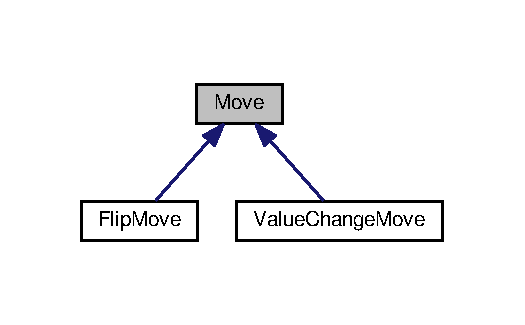
\includegraphics[width=252pt]{class_move__inherit__graph}
\end{center}
\end{figure}


Collaboration diagram for Move\-:\nopagebreak
\begin{figure}[H]
\begin{center}
\leavevmode
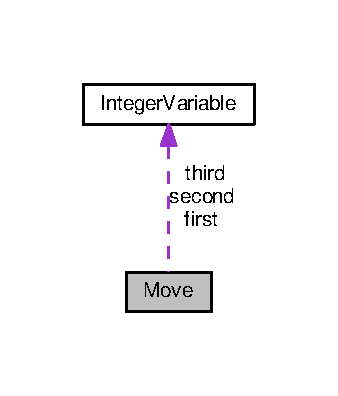
\includegraphics[width=162pt]{class_move__coll__graph}
\end{center}
\end{figure}
\subsection*{Public Member Functions}
\begin{DoxyCompactItemize}
\item 
\hyperlink{class_move_a4b1acc3a67d30c385ad9a6000526393a}{Move} ()
\item 
\hyperlink{class_move_a8851c92e7022c7c1958a01c5c4afaf9e}{Move} (\hyperlink{class_integer_variable}{Integer\-Variable} $\ast$var1, int delta1, int type)
\item 
\hyperlink{class_move_a2f898e7978074ce739c0c46d16b3917c}{Move} (\hyperlink{class_integer_variable}{Integer\-Variable} $\ast$var1, int delta1, \hyperlink{class_integer_variable}{Integer\-Variable} $\ast$var2, int delta2, int type)
\item 
\hyperlink{class_move_ab622b4f540b5d266677f61d2e4e6eff9}{Move} (\hyperlink{class_integer_variable}{Integer\-Variable} $\ast$var1, int delta1, \hyperlink{class_integer_variable}{Integer\-Variable} $\ast$var2, int delta2, \hyperlink{class_integer_variable}{Integer\-Variable} $\ast$var3, int delta3, int type)
\item 
void \hyperlink{class_move_a07a270da8300696c26e6614ef6c66065}{flip} ()
\item 
\hyperlink{class_move_aadd37321983fc477287bf7c6d1c0bacf}{$\sim$\-Move} ()
\item 
\hyperlink{class_move_a707f22adbcdc09ccb78e13f123a76c09}{Move} (const \hyperlink{class_move}{Move} \&a)
\item 
\hyperlink{class_move}{Move} \& \hyperlink{class_move_a3acc32180b60f853bd6445f3a3d84913}{operator=} (const \hyperlink{class_move}{Move} \&a)
\item 
void \hyperlink{class_move_a1438845e97365949d5550328f5aaadc7}{copy} (\hyperlink{class_move}{Move} $\ast$mv)
\end{DoxyCompactItemize}
\subsection*{Public Attributes}
\begin{DoxyCompactItemize}
\item 
\hyperlink{class_integer_variable}{Integer\-Variable} $\ast$ \hyperlink{class_move_ac4f4c8f895b197447e16b70c240b7746}{first}
\item 
int \hyperlink{class_move_ada1a03cd63710abd68c0e4505fe21f7e}{delta\-Value\-First}
\item 
\hyperlink{class_integer_variable}{Integer\-Variable} $\ast$ \hyperlink{class_move_ad2edb78f2d4533cdbc4d8f4ac5909d3f}{second}
\item 
int \hyperlink{class_move_af9a41af4cf88de2eb07d4601bbaf5011}{delta\-Value\-Second}
\item 
\hyperlink{class_integer_variable}{Integer\-Variable} $\ast$ \hyperlink{class_move_a255842251c3916ea715d5093797028c1}{third}
\item 
int \hyperlink{class_move_ad1d160b2033500b68a66337c7e13e657}{delta\-Value\-Third}
\item 
int \hyperlink{class_move_a5ffe8371cd87d9714122dacf913ae238}{move\-Type}
\end{DoxyCompactItemize}


\subsection{Constructor \& Destructor Documentation}
\hypertarget{class_move_a4b1acc3a67d30c385ad9a6000526393a}{\index{Move@{Move}!Move@{Move}}
\index{Move@{Move}!Move@{Move}}
\subsubsection[{Move}]{\setlength{\rightskip}{0pt plus 5cm}Move\-::\-Move (
\begin{DoxyParamCaption}
{}
\end{DoxyParamCaption}
)\hspace{0.3cm}{\ttfamily [inline]}}}\label{class_move_a4b1acc3a67d30c385ad9a6000526393a}
\hypertarget{class_move_a8851c92e7022c7c1958a01c5c4afaf9e}{\index{Move@{Move}!Move@{Move}}
\index{Move@{Move}!Move@{Move}}
\subsubsection[{Move}]{\setlength{\rightskip}{0pt plus 5cm}Move\-::\-Move (
\begin{DoxyParamCaption}
\item[{{\bf Integer\-Variable} $\ast$}]{var1, }
\item[{int}]{delta1, }
\item[{int}]{type}
\end{DoxyParamCaption}
)\hspace{0.3cm}{\ttfamily [inline]}}}\label{class_move_a8851c92e7022c7c1958a01c5c4afaf9e}
\hypertarget{class_move_a2f898e7978074ce739c0c46d16b3917c}{\index{Move@{Move}!Move@{Move}}
\index{Move@{Move}!Move@{Move}}
\subsubsection[{Move}]{\setlength{\rightskip}{0pt plus 5cm}Move\-::\-Move (
\begin{DoxyParamCaption}
\item[{{\bf Integer\-Variable} $\ast$}]{var1, }
\item[{int}]{delta1, }
\item[{{\bf Integer\-Variable} $\ast$}]{var2, }
\item[{int}]{delta2, }
\item[{int}]{type}
\end{DoxyParamCaption}
)\hspace{0.3cm}{\ttfamily [inline]}}}\label{class_move_a2f898e7978074ce739c0c46d16b3917c}
\hypertarget{class_move_ab622b4f540b5d266677f61d2e4e6eff9}{\index{Move@{Move}!Move@{Move}}
\index{Move@{Move}!Move@{Move}}
\subsubsection[{Move}]{\setlength{\rightskip}{0pt plus 5cm}Move\-::\-Move (
\begin{DoxyParamCaption}
\item[{{\bf Integer\-Variable} $\ast$}]{var1, }
\item[{int}]{delta1, }
\item[{{\bf Integer\-Variable} $\ast$}]{var2, }
\item[{int}]{delta2, }
\item[{{\bf Integer\-Variable} $\ast$}]{var3, }
\item[{int}]{delta3, }
\item[{int}]{type}
\end{DoxyParamCaption}
)\hspace{0.3cm}{\ttfamily [inline]}}}\label{class_move_ab622b4f540b5d266677f61d2e4e6eff9}
\hypertarget{class_move_aadd37321983fc477287bf7c6d1c0bacf}{\index{Move@{Move}!$\sim$\-Move@{$\sim$\-Move}}
\index{$\sim$\-Move@{$\sim$\-Move}!Move@{Move}}
\subsubsection[{$\sim$\-Move}]{\setlength{\rightskip}{0pt plus 5cm}Move\-::$\sim$\-Move (
\begin{DoxyParamCaption}
{}
\end{DoxyParamCaption}
)\hspace{0.3cm}{\ttfamily [inline]}}}\label{class_move_aadd37321983fc477287bf7c6d1c0bacf}
\hypertarget{class_move_a707f22adbcdc09ccb78e13f123a76c09}{\index{Move@{Move}!Move@{Move}}
\index{Move@{Move}!Move@{Move}}
\subsubsection[{Move}]{\setlength{\rightskip}{0pt plus 5cm}Move\-::\-Move (
\begin{DoxyParamCaption}
\item[{const {\bf Move} \&}]{a}
\end{DoxyParamCaption}
)\hspace{0.3cm}{\ttfamily [inline]}}}\label{class_move_a707f22adbcdc09ccb78e13f123a76c09}


\subsection{Member Function Documentation}
\hypertarget{class_move_a1438845e97365949d5550328f5aaadc7}{\index{Move@{Move}!copy@{copy}}
\index{copy@{copy}!Move@{Move}}
\subsubsection[{copy}]{\setlength{\rightskip}{0pt plus 5cm}void Move\-::copy (
\begin{DoxyParamCaption}
\item[{{\bf Move} $\ast$}]{mv}
\end{DoxyParamCaption}
)\hspace{0.3cm}{\ttfamily [inline]}}}\label{class_move_a1438845e97365949d5550328f5aaadc7}
\hypertarget{class_move_a07a270da8300696c26e6614ef6c66065}{\index{Move@{Move}!flip@{flip}}
\index{flip@{flip}!Move@{Move}}
\subsubsection[{flip}]{\setlength{\rightskip}{0pt plus 5cm}void Move\-::flip (
\begin{DoxyParamCaption}
{}
\end{DoxyParamCaption}
)\hspace{0.3cm}{\ttfamily [inline]}}}\label{class_move_a07a270da8300696c26e6614ef6c66065}
\hypertarget{class_move_a3acc32180b60f853bd6445f3a3d84913}{\index{Move@{Move}!operator=@{operator=}}
\index{operator=@{operator=}!Move@{Move}}
\subsubsection[{operator=}]{\setlength{\rightskip}{0pt plus 5cm}{\bf Move}\& Move\-::operator= (
\begin{DoxyParamCaption}
\item[{const {\bf Move} \&}]{a}
\end{DoxyParamCaption}
)\hspace{0.3cm}{\ttfamily [inline]}}}\label{class_move_a3acc32180b60f853bd6445f3a3d84913}


\subsection{Member Data Documentation}
\hypertarget{class_move_ada1a03cd63710abd68c0e4505fe21f7e}{\index{Move@{Move}!delta\-Value\-First@{delta\-Value\-First}}
\index{delta\-Value\-First@{delta\-Value\-First}!Move@{Move}}
\subsubsection[{delta\-Value\-First}]{\setlength{\rightskip}{0pt plus 5cm}int Move\-::delta\-Value\-First}}\label{class_move_ada1a03cd63710abd68c0e4505fe21f7e}
\hypertarget{class_move_af9a41af4cf88de2eb07d4601bbaf5011}{\index{Move@{Move}!delta\-Value\-Second@{delta\-Value\-Second}}
\index{delta\-Value\-Second@{delta\-Value\-Second}!Move@{Move}}
\subsubsection[{delta\-Value\-Second}]{\setlength{\rightskip}{0pt plus 5cm}int Move\-::delta\-Value\-Second}}\label{class_move_af9a41af4cf88de2eb07d4601bbaf5011}
\hypertarget{class_move_ad1d160b2033500b68a66337c7e13e657}{\index{Move@{Move}!delta\-Value\-Third@{delta\-Value\-Third}}
\index{delta\-Value\-Third@{delta\-Value\-Third}!Move@{Move}}
\subsubsection[{delta\-Value\-Third}]{\setlength{\rightskip}{0pt plus 5cm}int Move\-::delta\-Value\-Third}}\label{class_move_ad1d160b2033500b68a66337c7e13e657}
\hypertarget{class_move_ac4f4c8f895b197447e16b70c240b7746}{\index{Move@{Move}!first@{first}}
\index{first@{first}!Move@{Move}}
\subsubsection[{first}]{\setlength{\rightskip}{0pt plus 5cm}{\bf Integer\-Variable}$\ast$ Move\-::first}}\label{class_move_ac4f4c8f895b197447e16b70c240b7746}
\hypertarget{class_move_a5ffe8371cd87d9714122dacf913ae238}{\index{Move@{Move}!move\-Type@{move\-Type}}
\index{move\-Type@{move\-Type}!Move@{Move}}
\subsubsection[{move\-Type}]{\setlength{\rightskip}{0pt plus 5cm}int Move\-::move\-Type}}\label{class_move_a5ffe8371cd87d9714122dacf913ae238}
\hypertarget{class_move_ad2edb78f2d4533cdbc4d8f4ac5909d3f}{\index{Move@{Move}!second@{second}}
\index{second@{second}!Move@{Move}}
\subsubsection[{second}]{\setlength{\rightskip}{0pt plus 5cm}{\bf Integer\-Variable}$\ast$ Move\-::second}}\label{class_move_ad2edb78f2d4533cdbc4d8f4ac5909d3f}
\hypertarget{class_move_a255842251c3916ea715d5093797028c1}{\index{Move@{Move}!third@{third}}
\index{third@{third}!Move@{Move}}
\subsubsection[{third}]{\setlength{\rightskip}{0pt plus 5cm}{\bf Integer\-Variable}$\ast$ Move\-::third}}\label{class_move_a255842251c3916ea715d5093797028c1}


The documentation for this class was generated from the following file\-:\begin{DoxyCompactItemize}
\item 
\hyperlink{_move_8hpp}{Move.\-hpp}\end{DoxyCompactItemize}

\hypertarget{class_multistop}{\section{Multistop Class Reference}
\label{class_multistop}\index{Multistop@{Multistop}}
}


{\ttfamily \#include $<$Multistop.\-hpp$>$}



Inheritance diagram for Multistop\-:\nopagebreak
\begin{figure}[H]
\begin{center}
\leavevmode
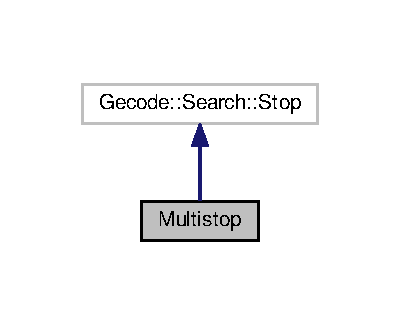
\includegraphics[width=192pt]{class_multistop__inherit__graph}
\end{center}
\end{figure}


Collaboration diagram for Multistop\-:\nopagebreak
\begin{figure}[H]
\begin{center}
\leavevmode
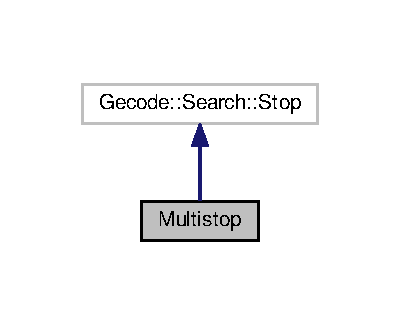
\includegraphics[width=192pt]{class_multistop__coll__graph}
\end{center}
\end{figure}
\subsection*{Public Member Functions}
\begin{DoxyCompactItemize}
\item 
\hyperlink{class_multistop_a6ea7ec76f1a44b19b96813f4f772678a}{Multistop} (unsigned node, unsigned fail, unsigned time)
\item 
virtual bool \hyperlink{class_multistop_ac50ce86548b5af2aaa159da80f1aa2f6}{stop} (const Gecode\-::\-Search\-::\-Statistics \&s, const Gecode\-::\-Search\-::\-Options \&o)
\begin{DoxyCompactList}\small\item\em Return true if node, time or fail limit is exceeded. \end{DoxyCompactList}\item 
\hyperlink{class_multistop_a6ad6831344419f22b4be9cf7c093f47b}{Multistop} (const \hyperlink{class_multistop}{Multistop} \&orig)
\item 
\hyperlink{class_multistop_a2eded054110488245670f926337cd1ed}{$\sim$\-Multistop} ()
\end{DoxyCompactItemize}
\subsection*{Public Attributes}
\begin{DoxyCompactItemize}
\item 
int \hyperlink{class_multistop_a46f7c2d55ad60df362d8551fe7a983ef}{called} = 0
\end{DoxyCompactItemize}
\subsection*{Private Attributes}
\begin{DoxyCompactItemize}
\item 
Gecode\-::\-Search\-::\-Node\-Stop $\ast$ \hyperlink{class_multistop_a7fa3af8c2fa7fb4758dc77016f462386}{ns}
\begin{DoxyCompactList}\small\item\em Used node stop object. \end{DoxyCompactList}\item 
Gecode\-::\-Search\-::\-Fail\-Stop $\ast$ \hyperlink{class_multistop_a8c29d6895a4be86afd7b3ebdad00369a}{fs}
\begin{DoxyCompactList}\small\item\em Used fail stop object. \end{DoxyCompactList}\item 
Gecode\-::\-Search\-::\-Time\-Stop $\ast$ \hyperlink{class_multistop_a6cf22f443f85c506ef15bdfd494bfb2a}{ts}
\begin{DoxyCompactList}\small\item\em Used time stop object. \end{DoxyCompactList}\end{DoxyCompactItemize}


\subsection{Constructor \& Destructor Documentation}
\hypertarget{class_multistop_a6ea7ec76f1a44b19b96813f4f772678a}{\index{Multistop@{Multistop}!Multistop@{Multistop}}
\index{Multistop@{Multistop}!Multistop@{Multistop}}
\subsubsection[{Multistop}]{\setlength{\rightskip}{0pt plus 5cm}Multistop\-::\-Multistop (
\begin{DoxyParamCaption}
\item[{unsigned}]{node, }
\item[{unsigned}]{fail, }
\item[{unsigned}]{time}
\end{DoxyParamCaption}
)}}\label{class_multistop_a6ea7ec76f1a44b19b96813f4f772678a}
Creates a Stop object with three stop criteria node, fail, and time. Giving 0 as an argument will ignorer that criteria. Time is in ms. \hypertarget{class_multistop_a6ad6831344419f22b4be9cf7c093f47b}{\index{Multistop@{Multistop}!Multistop@{Multistop}}
\index{Multistop@{Multistop}!Multistop@{Multistop}}
\subsubsection[{Multistop}]{\setlength{\rightskip}{0pt plus 5cm}Multistop\-::\-Multistop (
\begin{DoxyParamCaption}
\item[{const {\bf Multistop} \&}]{orig}
\end{DoxyParamCaption}
)}}\label{class_multistop_a6ad6831344419f22b4be9cf7c093f47b}
\hypertarget{class_multistop_a2eded054110488245670f926337cd1ed}{\index{Multistop@{Multistop}!$\sim$\-Multistop@{$\sim$\-Multistop}}
\index{$\sim$\-Multistop@{$\sim$\-Multistop}!Multistop@{Multistop}}
\subsubsection[{$\sim$\-Multistop}]{\setlength{\rightskip}{0pt plus 5cm}Multistop\-::$\sim$\-Multistop (
\begin{DoxyParamCaption}
{}
\end{DoxyParamCaption}
)}}\label{class_multistop_a2eded054110488245670f926337cd1ed}


\subsection{Member Function Documentation}
\hypertarget{class_multistop_ac50ce86548b5af2aaa159da80f1aa2f6}{\index{Multistop@{Multistop}!stop@{stop}}
\index{stop@{stop}!Multistop@{Multistop}}
\subsubsection[{stop}]{\setlength{\rightskip}{0pt plus 5cm}bool Multistop\-::stop (
\begin{DoxyParamCaption}
\item[{const Gecode\-::\-Search\-::\-Statistics \&}]{s, }
\item[{const Gecode\-::\-Search\-::\-Options \&}]{o}
\end{DoxyParamCaption}
)\hspace{0.3cm}{\ttfamily [virtual]}}}\label{class_multistop_ac50ce86548b5af2aaa159da80f1aa2f6}


Return true if node, time or fail limit is exceeded. 



\subsection{Member Data Documentation}
\hypertarget{class_multistop_a46f7c2d55ad60df362d8551fe7a983ef}{\index{Multistop@{Multistop}!called@{called}}
\index{called@{called}!Multistop@{Multistop}}
\subsubsection[{called}]{\setlength{\rightskip}{0pt plus 5cm}int Multistop\-::called = 0}}\label{class_multistop_a46f7c2d55ad60df362d8551fe7a983ef}
\hypertarget{class_multistop_a8c29d6895a4be86afd7b3ebdad00369a}{\index{Multistop@{Multistop}!fs@{fs}}
\index{fs@{fs}!Multistop@{Multistop}}
\subsubsection[{fs}]{\setlength{\rightskip}{0pt plus 5cm}Gecode\-::\-Search\-::\-Fail\-Stop$\ast$ Multistop\-::fs\hspace{0.3cm}{\ttfamily [private]}}}\label{class_multistop_a8c29d6895a4be86afd7b3ebdad00369a}


Used fail stop object. 

\hypertarget{class_multistop_a7fa3af8c2fa7fb4758dc77016f462386}{\index{Multistop@{Multistop}!ns@{ns}}
\index{ns@{ns}!Multistop@{Multistop}}
\subsubsection[{ns}]{\setlength{\rightskip}{0pt plus 5cm}Gecode\-::\-Search\-::\-Node\-Stop$\ast$ Multistop\-::ns\hspace{0.3cm}{\ttfamily [private]}}}\label{class_multistop_a7fa3af8c2fa7fb4758dc77016f462386}


Used node stop object. 

\hypertarget{class_multistop_a6cf22f443f85c506ef15bdfd494bfb2a}{\index{Multistop@{Multistop}!ts@{ts}}
\index{ts@{ts}!Multistop@{Multistop}}
\subsubsection[{ts}]{\setlength{\rightskip}{0pt plus 5cm}Gecode\-::\-Search\-::\-Time\-Stop$\ast$ Multistop\-::ts\hspace{0.3cm}{\ttfamily [private]}}}\label{class_multistop_a6cf22f443f85c506ef15bdfd494bfb2a}


Used time stop object. 



The documentation for this class was generated from the following files\-:\begin{DoxyCompactItemize}
\item 
\hyperlink{_multistop_8hpp}{Multistop.\-hpp}\item 
\hyperlink{_multistop_8cpp}{Multistop.\-cpp}\end{DoxyCompactItemize}

\hypertarget{class_neighborhood_explorer}{\section{Neighborhood\-Explorer Class Reference}
\label{class_neighborhood_explorer}\index{Neighborhood\-Explorer@{Neighborhood\-Explorer}}
}


{\ttfamily \#include $<$Neighborhood\-Explorer.\-hpp$>$}

\subsection*{Public Member Functions}
\begin{DoxyCompactItemize}
\item 
\hyperlink{class_neighborhood_explorer_a1d4c826b5d812cb8a6e4d8371e8b8e5a}{Neighborhood\-Explorer} (std\-::shared\-\_\-ptr$<$ \hyperlink{class_model}{Model} $>$ \hyperlink{class_neighborhood_explorer_aa4da40077758b18ef280c1fba3d9092e}{model})
\item 
\hyperlink{class_neighborhood_explorer_afe9eb7ec443d05d2f2b43695fed74b06}{Neighborhood\-Explorer} (const \hyperlink{class_neighborhood_explorer}{Neighborhood\-Explorer} \&orig)
\item 
virtual \hyperlink{class_neighborhood_explorer_a477dff82a42d89438c5b21a87874062c}{$\sim$\-Neighborhood\-Explorer} ()
\item 
void \hyperlink{class_neighborhood_explorer_a56eb7d36d136801c1d7b9e39a2f9ccfb}{random\-Walk} (\hyperlink{class_move}{Move} $\ast$mv, std\-::shared\-\_\-ptr$<$ \hyperlink{class_state}{State} $>$ st)
\item 
bool \hyperlink{class_neighborhood_explorer_a8c30c890d40d19c8c0eb1f4a3285c3b0}{best\-Improvement} (\hyperlink{class_move}{Move} $\ast$mv, std\-::shared\-\_\-ptr$<$ \hyperlink{class_state}{State} $>$ st)
\item 
void \hyperlink{class_neighborhood_explorer_adab61e4e07cb283e90ebbf9a19826969}{make\-Move} (\hyperlink{class_move}{Move} $\ast$mv, std\-::shared\-\_\-ptr$<$ \hyperlink{class_state}{State} $>$ st)
\end{DoxyCompactItemize}
\subsection*{Public Attributes}
\begin{DoxyCompactItemize}
\item 
std\-::shared\-\_\-ptr$<$ \hyperlink{class_model}{Model} $>$ \hyperlink{class_neighborhood_explorer_aa4da40077758b18ef280c1fba3d9092e}{model}
\end{DoxyCompactItemize}
\subsection*{Private Member Functions}
\begin{DoxyCompactItemize}
\item 
std\-::vector$<$ int $>$ \hyperlink{class_neighborhood_explorer_abfd048806a7d347a426627b501cbd064}{calculate\-Delta\-Change} (\hyperlink{class_move}{Move} $\ast$mv)
\begin{DoxyCompactList}\small\item\em Not using priority of constraints yet. \end{DoxyCompactList}\item 
void \hyperlink{class_neighborhood_explorer_ab2746ffea7415f67c086f467a94bb361}{commit\-Move} (\hyperlink{class_move}{Move} $\ast$mv, std\-::shared\-\_\-ptr$<$ \hyperlink{class_state}{State} $>$ st)
\end{DoxyCompactItemize}


\subsection{Constructor \& Destructor Documentation}
\hypertarget{class_neighborhood_explorer_a1d4c826b5d812cb8a6e4d8371e8b8e5a}{\index{Neighborhood\-Explorer@{Neighborhood\-Explorer}!Neighborhood\-Explorer@{Neighborhood\-Explorer}}
\index{Neighborhood\-Explorer@{Neighborhood\-Explorer}!NeighborhoodExplorer@{Neighborhood\-Explorer}}
\subsubsection[{Neighborhood\-Explorer}]{\setlength{\rightskip}{0pt plus 5cm}Neighborhood\-Explorer\-::\-Neighborhood\-Explorer (
\begin{DoxyParamCaption}
\item[{std\-::shared\-\_\-ptr$<$ {\bf Model} $>$}]{model}
\end{DoxyParamCaption}
)}}\label{class_neighborhood_explorer_a1d4c826b5d812cb8a6e4d8371e8b8e5a}
\hypertarget{class_neighborhood_explorer_afe9eb7ec443d05d2f2b43695fed74b06}{\index{Neighborhood\-Explorer@{Neighborhood\-Explorer}!Neighborhood\-Explorer@{Neighborhood\-Explorer}}
\index{Neighborhood\-Explorer@{Neighborhood\-Explorer}!NeighborhoodExplorer@{Neighborhood\-Explorer}}
\subsubsection[{Neighborhood\-Explorer}]{\setlength{\rightskip}{0pt plus 5cm}Neighborhood\-Explorer\-::\-Neighborhood\-Explorer (
\begin{DoxyParamCaption}
\item[{const {\bf Neighborhood\-Explorer} \&}]{orig}
\end{DoxyParamCaption}
)}}\label{class_neighborhood_explorer_afe9eb7ec443d05d2f2b43695fed74b06}
\hypertarget{class_neighborhood_explorer_a477dff82a42d89438c5b21a87874062c}{\index{Neighborhood\-Explorer@{Neighborhood\-Explorer}!$\sim$\-Neighborhood\-Explorer@{$\sim$\-Neighborhood\-Explorer}}
\index{$\sim$\-Neighborhood\-Explorer@{$\sim$\-Neighborhood\-Explorer}!NeighborhoodExplorer@{Neighborhood\-Explorer}}
\subsubsection[{$\sim$\-Neighborhood\-Explorer}]{\setlength{\rightskip}{0pt plus 5cm}Neighborhood\-Explorer\-::$\sim$\-Neighborhood\-Explorer (
\begin{DoxyParamCaption}
{}
\end{DoxyParamCaption}
)\hspace{0.3cm}{\ttfamily [virtual]}}}\label{class_neighborhood_explorer_a477dff82a42d89438c5b21a87874062c}


\subsection{Member Function Documentation}
\hypertarget{class_neighborhood_explorer_a8c30c890d40d19c8c0eb1f4a3285c3b0}{\index{Neighborhood\-Explorer@{Neighborhood\-Explorer}!best\-Improvement@{best\-Improvement}}
\index{best\-Improvement@{best\-Improvement}!NeighborhoodExplorer@{Neighborhood\-Explorer}}
\subsubsection[{best\-Improvement}]{\setlength{\rightskip}{0pt plus 5cm}bool Neighborhood\-Explorer\-::best\-Improvement (
\begin{DoxyParamCaption}
\item[{{\bf Move} $\ast$}]{mv, }
\item[{std\-::shared\-\_\-ptr$<$ {\bf State} $>$}]{st}
\end{DoxyParamCaption}
)}}\label{class_neighborhood_explorer_a8c30c890d40d19c8c0eb1f4a3285c3b0}
\hypertarget{class_neighborhood_explorer_abfd048806a7d347a426627b501cbd064}{\index{Neighborhood\-Explorer@{Neighborhood\-Explorer}!calculate\-Delta\-Change@{calculate\-Delta\-Change}}
\index{calculate\-Delta\-Change@{calculate\-Delta\-Change}!NeighborhoodExplorer@{Neighborhood\-Explorer}}
\subsubsection[{calculate\-Delta\-Change}]{\setlength{\rightskip}{0pt plus 5cm}std\-::vector$<$ int $>$ Neighborhood\-Explorer\-::calculate\-Delta\-Change (
\begin{DoxyParamCaption}
\item[{{\bf Move} $\ast$}]{mv}
\end{DoxyParamCaption}
)\hspace{0.3cm}{\ttfamily [private]}}}\label{class_neighborhood_explorer_abfd048806a7d347a426627b501cbd064}


Not using priority of constraints yet. 

\hypertarget{class_neighborhood_explorer_ab2746ffea7415f67c086f467a94bb361}{\index{Neighborhood\-Explorer@{Neighborhood\-Explorer}!commit\-Move@{commit\-Move}}
\index{commit\-Move@{commit\-Move}!NeighborhoodExplorer@{Neighborhood\-Explorer}}
\subsubsection[{commit\-Move}]{\setlength{\rightskip}{0pt plus 5cm}void Neighborhood\-Explorer\-::commit\-Move (
\begin{DoxyParamCaption}
\item[{{\bf Move} $\ast$}]{mv, }
\item[{std\-::shared\-\_\-ptr$<$ {\bf State} $>$}]{st}
\end{DoxyParamCaption}
)\hspace{0.3cm}{\ttfamily [private]}}}\label{class_neighborhood_explorer_ab2746ffea7415f67c086f467a94bb361}
\hypertarget{class_neighborhood_explorer_adab61e4e07cb283e90ebbf9a19826969}{\index{Neighborhood\-Explorer@{Neighborhood\-Explorer}!make\-Move@{make\-Move}}
\index{make\-Move@{make\-Move}!NeighborhoodExplorer@{Neighborhood\-Explorer}}
\subsubsection[{make\-Move}]{\setlength{\rightskip}{0pt plus 5cm}void Neighborhood\-Explorer\-::make\-Move (
\begin{DoxyParamCaption}
\item[{{\bf Move} $\ast$}]{mv, }
\item[{std\-::shared\-\_\-ptr$<$ {\bf State} $>$}]{st}
\end{DoxyParamCaption}
)}}\label{class_neighborhood_explorer_adab61e4e07cb283e90ebbf9a19826969}
\hypertarget{class_neighborhood_explorer_a56eb7d36d136801c1d7b9e39a2f9ccfb}{\index{Neighborhood\-Explorer@{Neighborhood\-Explorer}!random\-Walk@{random\-Walk}}
\index{random\-Walk@{random\-Walk}!NeighborhoodExplorer@{Neighborhood\-Explorer}}
\subsubsection[{random\-Walk}]{\setlength{\rightskip}{0pt plus 5cm}void Neighborhood\-Explorer\-::random\-Walk (
\begin{DoxyParamCaption}
\item[{{\bf Move} $\ast$}]{mv, }
\item[{std\-::shared\-\_\-ptr$<$ {\bf State} $>$}]{st}
\end{DoxyParamCaption}
)}}\label{class_neighborhood_explorer_a56eb7d36d136801c1d7b9e39a2f9ccfb}


\subsection{Member Data Documentation}
\hypertarget{class_neighborhood_explorer_aa4da40077758b18ef280c1fba3d9092e}{\index{Neighborhood\-Explorer@{Neighborhood\-Explorer}!model@{model}}
\index{model@{model}!NeighborhoodExplorer@{Neighborhood\-Explorer}}
\subsubsection[{model}]{\setlength{\rightskip}{0pt plus 5cm}std\-::shared\-\_\-ptr$<${\bf Model}$>$ Neighborhood\-Explorer\-::model}}\label{class_neighborhood_explorer_aa4da40077758b18ef280c1fba3d9092e}


The documentation for this class was generated from the following files\-:\begin{DoxyCompactItemize}
\item 
\hyperlink{_neighborhood_explorer_8hpp}{Neighborhood\-Explorer.\-hpp}\item 
\hyperlink{_neighborhood_explorer_8cpp}{Neighborhood\-Explorer.\-cpp}\end{DoxyCompactItemize}

\hypertarget{class_options}{\section{Options Class Reference}
\label{class_options}\index{Options@{Options}}
}


{\ttfamily \#include $<$Options.\-hpp$>$}

\subsection*{Public Member Functions}
\begin{DoxyCompactItemize}
\item 
\hyperlink{class_options_ab72fb640172a6109e34c8a5366563753}{Options} ()
\item 
\hyperlink{class_options_a71b507295fe472af25f6b2baaf1443ee}{Options} (const \hyperlink{class_options}{Options} \&orig)
\item 
virtual \hyperlink{class_options_a86ddb85b183f8b58af5481f30a42fa92}{$\sim$\-Options} ()
\end{DoxyCompactItemize}
\subsection*{Private Attributes}
\begin{DoxyCompactItemize}
\item 
ínt \hyperlink{class_options_a5d93595f2e16b3126a263244ddf85a43}{timelimit} = 0
\end{DoxyCompactItemize}


\subsection{Constructor \& Destructor Documentation}
\hypertarget{class_options_ab72fb640172a6109e34c8a5366563753}{\index{Options@{Options}!Options@{Options}}
\index{Options@{Options}!Options@{Options}}
\subsubsection[{Options}]{\setlength{\rightskip}{0pt plus 5cm}Options\-::\-Options (
\begin{DoxyParamCaption}
{}
\end{DoxyParamCaption}
)}}\label{class_options_ab72fb640172a6109e34c8a5366563753}
\hypertarget{class_options_a71b507295fe472af25f6b2baaf1443ee}{\index{Options@{Options}!Options@{Options}}
\index{Options@{Options}!Options@{Options}}
\subsubsection[{Options}]{\setlength{\rightskip}{0pt plus 5cm}Options\-::\-Options (
\begin{DoxyParamCaption}
\item[{const {\bf Options} \&}]{orig}
\end{DoxyParamCaption}
)}}\label{class_options_a71b507295fe472af25f6b2baaf1443ee}
\hypertarget{class_options_a86ddb85b183f8b58af5481f30a42fa92}{\index{Options@{Options}!$\sim$\-Options@{$\sim$\-Options}}
\index{$\sim$\-Options@{$\sim$\-Options}!Options@{Options}}
\subsubsection[{$\sim$\-Options}]{\setlength{\rightskip}{0pt plus 5cm}Options\-::$\sim$\-Options (
\begin{DoxyParamCaption}
{}
\end{DoxyParamCaption}
)\hspace{0.3cm}{\ttfamily [virtual]}}}\label{class_options_a86ddb85b183f8b58af5481f30a42fa92}


\subsection{Member Data Documentation}
\hypertarget{class_options_a5d93595f2e16b3126a263244ddf85a43}{\index{Options@{Options}!timelimit@{timelimit}}
\index{timelimit@{timelimit}!Options@{Options}}
\subsubsection[{timelimit}]{\setlength{\rightskip}{0pt plus 5cm}ínt Options\-::timelimit = 0\hspace{0.3cm}{\ttfamily [private]}}}\label{class_options_a5d93595f2e16b3126a263244ddf85a43}


The documentation for this class was generated from the following files\-:\begin{DoxyCompactItemize}
\item 
\hyperlink{_options_8hpp}{Options.\-hpp}\item 
\hyperlink{_options_8cpp}{Options.\-cpp}\end{DoxyCompactItemize}

\hypertarget{class_random}{\section{Random Class Reference}
\label{class_random}\index{Random@{Random}}
}


{\ttfamily \#include $<$Random.\-hpp$>$}

\subsection*{Static Public Member Functions}
\begin{DoxyCompactItemize}
\item 
static int \hyperlink{class_random_aa56a13c81680b43082ff2c29c2488212}{Integer} (int lb, int ub)
\item 
static int \hyperlink{class_random_afd2386359635f5e79df7108bdf288c86}{Integer} (int ub)
\item 
static double \hyperlink{class_random_a913483b8b2d33a4b8aa60b64749ed434}{Double} (double lb=0, double ub=1)
\item 
static int \hyperlink{class_random_a032603d2d9246b9d5f140fb8ba03276e}{Seed} (int \hyperlink{class_random_a046dccc4dc6055ffd3e90d597beb8620}{seed})
\end{DoxyCompactItemize}
\subsection*{Static Public Attributes}
\begin{DoxyCompactItemize}
\item 
static std\-::mt19937 \hyperlink{class_random_aa4354db31fa7d64040939b905ab12ee1}{mt}
\item 
static int \hyperlink{class_random_a046dccc4dc6055ffd3e90d597beb8620}{seed} = std\-::random\-\_\-device()()
\end{DoxyCompactItemize}


\subsection{Member Function Documentation}
\hypertarget{class_random_a913483b8b2d33a4b8aa60b64749ed434}{\index{Random@{Random}!Double@{Double}}
\index{Double@{Double}!Random@{Random}}
\subsubsection[{Double}]{\setlength{\rightskip}{0pt plus 5cm}double Random\-::\-Double (
\begin{DoxyParamCaption}
\item[{double}]{lb = {\ttfamily 0}, }
\item[{double}]{ub = {\ttfamily 1}}
\end{DoxyParamCaption}
)\hspace{0.3cm}{\ttfamily [static]}}}\label{class_random_a913483b8b2d33a4b8aa60b64749ed434}
\hypertarget{class_random_aa56a13c81680b43082ff2c29c2488212}{\index{Random@{Random}!Integer@{Integer}}
\index{Integer@{Integer}!Random@{Random}}
\subsubsection[{Integer}]{\setlength{\rightskip}{0pt plus 5cm}int Random\-::\-Integer (
\begin{DoxyParamCaption}
\item[{int}]{lb, }
\item[{int}]{ub}
\end{DoxyParamCaption}
)\hspace{0.3cm}{\ttfamily [static]}}}\label{class_random_aa56a13c81680b43082ff2c29c2488212}
\hypertarget{class_random_afd2386359635f5e79df7108bdf288c86}{\index{Random@{Random}!Integer@{Integer}}
\index{Integer@{Integer}!Random@{Random}}
\subsubsection[{Integer}]{\setlength{\rightskip}{0pt plus 5cm}int Random\-::\-Integer (
\begin{DoxyParamCaption}
\item[{int}]{ub}
\end{DoxyParamCaption}
)\hspace{0.3cm}{\ttfamily [static]}}}\label{class_random_afd2386359635f5e79df7108bdf288c86}
\hypertarget{class_random_a032603d2d9246b9d5f140fb8ba03276e}{\index{Random@{Random}!Seed@{Seed}}
\index{Seed@{Seed}!Random@{Random}}
\subsubsection[{Seed}]{\setlength{\rightskip}{0pt plus 5cm}int Random\-::\-Seed (
\begin{DoxyParamCaption}
\item[{int}]{seed}
\end{DoxyParamCaption}
)\hspace{0.3cm}{\ttfamily [static]}}}\label{class_random_a032603d2d9246b9d5f140fb8ba03276e}


\subsection{Member Data Documentation}
\hypertarget{class_random_aa4354db31fa7d64040939b905ab12ee1}{\index{Random@{Random}!mt@{mt}}
\index{mt@{mt}!Random@{Random}}
\subsubsection[{mt}]{\setlength{\rightskip}{0pt plus 5cm}std\-::mt19937 Random\-::mt\hspace{0.3cm}{\ttfamily [static]}}}\label{class_random_aa4354db31fa7d64040939b905ab12ee1}
\hypertarget{class_random_a046dccc4dc6055ffd3e90d597beb8620}{\index{Random@{Random}!seed@{seed}}
\index{seed@{seed}!Random@{Random}}
\subsubsection[{seed}]{\setlength{\rightskip}{0pt plus 5cm}int Random\-::seed = std\-::random\-\_\-device()()\hspace{0.3cm}{\ttfamily [static]}}}\label{class_random_a046dccc4dc6055ffd3e90d597beb8620}


The documentation for this class was generated from the following files\-:\begin{DoxyCompactItemize}
\item 
\hyperlink{_random_8hpp}{Random.\-hpp}\item 
\hyperlink{_random_8cpp}{Random.\-cpp}\end{DoxyCompactItemize}

\hypertarget{struct_constraint_1_1_sort_greater}{\section{Constraint\-:\-:Sort\-Greater Struct Reference}
\label{struct_constraint_1_1_sort_greater}\index{Constraint\-::\-Sort\-Greater@{Constraint\-::\-Sort\-Greater}}
}


{\ttfamily \#include $<$Constraint.\-hpp$>$}

\subsection*{Public Member Functions}
\begin{DoxyCompactItemize}
\item 
bool \hyperlink{struct_constraint_1_1_sort_greater_a64a3f436d2babc91f707754c04648ae2}{operator()} (const std\-::shared\-\_\-ptr$<$ \hyperlink{class_constraint}{Constraint} $>$ \&cons1, const std\-::shared\-\_\-ptr$<$ \hyperlink{class_constraint}{Constraint} $>$ \&cons2) const 
\end{DoxyCompactItemize}


\subsection{Member Function Documentation}
\hypertarget{struct_constraint_1_1_sort_greater_a64a3f436d2babc91f707754c04648ae2}{\index{Constraint\-::\-Sort\-Greater@{Constraint\-::\-Sort\-Greater}!operator()@{operator()}}
\index{operator()@{operator()}!Constraint::SortGreater@{Constraint\-::\-Sort\-Greater}}
\subsubsection[{operator()}]{\setlength{\rightskip}{0pt plus 5cm}bool Constraint\-::\-Sort\-Greater\-::operator() (
\begin{DoxyParamCaption}
\item[{const std\-::shared\-\_\-ptr$<$ {\bf Constraint} $>$ \&}]{cons1, }
\item[{const std\-::shared\-\_\-ptr$<$ {\bf Constraint} $>$ \&}]{cons2}
\end{DoxyParamCaption}
) const\hspace{0.3cm}{\ttfamily [inline]}}}\label{struct_constraint_1_1_sort_greater_a64a3f436d2babc91f707754c04648ae2}


The documentation for this struct was generated from the following file\-:\begin{DoxyCompactItemize}
\item 
\hyperlink{_constraint_8hpp}{Constraint.\-hpp}\end{DoxyCompactItemize}

\hypertarget{class_state}{\section{State Class Reference}
\label{class_state}\index{State@{State}}
}


{\ttfamily \#include $<$State.\-hpp$>$}

\subsection*{Public Member Functions}
\begin{DoxyCompactItemize}
\item 
\hyperlink{class_state_a96b1ea641bbd8a6f6307e8746b8e661e}{State} (std\-::shared\-\_\-ptr$<$ \hyperlink{class_model}{Model} $>$ \hyperlink{class_state_a186c5e2023a2fe5f0587c77e55f122a9}{model})
\item 
\hyperlink{class_state_ae26524535e8d9942d3e6c366034871b2}{State} (const \hyperlink{class_state}{State} \&orig)
\item 
virtual \hyperlink{class_state_afab438d92b90dc18d194dbd9c9c8bab3}{$\sim$\-State} ()
\item 
void \hyperlink{class_state_aa0dbbbff73846072ab4a395ab376eeb7}{initialize\-Invariants} ()
\begin{DoxyCompactList}\small\item\em Maybe all the initialize should be moved to model (again). \end{DoxyCompactList}\item 
void \hyperlink{class_state_a75fc5012815b887e31dc9c5e62520fd4}{initialize\-Constraints} ()
\item 
void \hyperlink{class_state_aa1af926682cee09f6074833856adba10}{initialize\-Objective} ()
\item 
int \hyperlink{class_state_a1deb2567ba6e2e1bf292658db671b5bd}{get\-Objective\-Value} ()
\item 
void \hyperlink{class_state_a73295654a3879aa1651543156d4cad9e}{save\-Solution} ()
\item 
std\-::vector$<$ int $>$ $\ast$ \hyperlink{class_state_a51ba8c2241ed349b83e5e46f30c0a0ba}{get\-Solution} ()
\item 
int \hyperlink{class_state_aa75ca0e6a38f66db9365e32c035d992e}{get\-Solution\-Value} ()
\item 
void \hyperlink{class_state_a9d4048063f30a838bf430ffb7ecdfbc7}{set\-Solution} ()
\item 
bool \hyperlink{class_state_a7efd4a9d3bb0a2d285421e7cf847e826}{recalculate\-All} ()
\item 
int \hyperlink{class_state_a3f1b234c71d5b092f461cabb3a2dbb62}{mask\-At} (int i)
\begin{DoxyCompactList}\small\item\em \hyperlink{class_move}{Move} this to model. \end{DoxyCompactList}\item 
void \hyperlink{class_state_ab501d958f58c45daaea79337884dee09}{shuffle\-Mask} ()
\begin{DoxyCompactList}\small\item\em \hyperlink{class_move}{Move} this to model. \end{DoxyCompactList}\end{DoxyCompactItemize}
\subsection*{Public Attributes}
\begin{DoxyCompactItemize}
\item 
int \hyperlink{class_state_a1486bf81e466cab8d70d3b550cd4e0f9}{number\-Of\-Violations}
\end{DoxyCompactItemize}
\subsection*{Private Attributes}
\begin{DoxyCompactItemize}
\item 
int \hyperlink{class_state_a1cd5b1a0b71c43d2da0dfff6147f245c}{solution\-Value}
\item 
std\-::vector$<$ int $>$ $\ast$ \hyperlink{class_state_af719cb2cc33bb43091fd40ee0d6b5bf9}{mask}
\item 
std\-::shared\-\_\-ptr$<$ \hyperlink{class_model}{Model} $>$ \hyperlink{class_state_a186c5e2023a2fe5f0587c77e55f122a9}{model}
\item 
std\-::vector$<$ int $>$ $\ast$ \hyperlink{class_state_aa37c4277fe2f3be05931b7a5b8443401}{solution}
\end{DoxyCompactItemize}


\subsection{Constructor \& Destructor Documentation}
\hypertarget{class_state_a96b1ea641bbd8a6f6307e8746b8e661e}{\index{State@{State}!State@{State}}
\index{State@{State}!State@{State}}
\subsubsection[{State}]{\setlength{\rightskip}{0pt plus 5cm}State\-::\-State (
\begin{DoxyParamCaption}
\item[{std\-::shared\-\_\-ptr$<$ {\bf Model} $>$}]{model}
\end{DoxyParamCaption}
)}}\label{class_state_a96b1ea641bbd8a6f6307e8746b8e661e}
\hypertarget{class_state_ae26524535e8d9942d3e6c366034871b2}{\index{State@{State}!State@{State}}
\index{State@{State}!State@{State}}
\subsubsection[{State}]{\setlength{\rightskip}{0pt plus 5cm}State\-::\-State (
\begin{DoxyParamCaption}
\item[{const {\bf State} \&}]{orig}
\end{DoxyParamCaption}
)}}\label{class_state_ae26524535e8d9942d3e6c366034871b2}
\hypertarget{class_state_afab438d92b90dc18d194dbd9c9c8bab3}{\index{State@{State}!$\sim$\-State@{$\sim$\-State}}
\index{$\sim$\-State@{$\sim$\-State}!State@{State}}
\subsubsection[{$\sim$\-State}]{\setlength{\rightskip}{0pt plus 5cm}State\-::$\sim$\-State (
\begin{DoxyParamCaption}
{}
\end{DoxyParamCaption}
)\hspace{0.3cm}{\ttfamily [virtual]}}}\label{class_state_afab438d92b90dc18d194dbd9c9c8bab3}


\subsection{Member Function Documentation}
\hypertarget{class_state_a1deb2567ba6e2e1bf292658db671b5bd}{\index{State@{State}!get\-Objective\-Value@{get\-Objective\-Value}}
\index{get\-Objective\-Value@{get\-Objective\-Value}!State@{State}}
\subsubsection[{get\-Objective\-Value}]{\setlength{\rightskip}{0pt plus 5cm}int State\-::get\-Objective\-Value (
\begin{DoxyParamCaption}
{}
\end{DoxyParamCaption}
)}}\label{class_state_a1deb2567ba6e2e1bf292658db671b5bd}
\hypertarget{class_state_a51ba8c2241ed349b83e5e46f30c0a0ba}{\index{State@{State}!get\-Solution@{get\-Solution}}
\index{get\-Solution@{get\-Solution}!State@{State}}
\subsubsection[{get\-Solution}]{\setlength{\rightskip}{0pt plus 5cm}std\-::vector$<$ int $>$ $\ast$ State\-::get\-Solution (
\begin{DoxyParamCaption}
{}
\end{DoxyParamCaption}
)}}\label{class_state_a51ba8c2241ed349b83e5e46f30c0a0ba}
\hypertarget{class_state_aa75ca0e6a38f66db9365e32c035d992e}{\index{State@{State}!get\-Solution\-Value@{get\-Solution\-Value}}
\index{get\-Solution\-Value@{get\-Solution\-Value}!State@{State}}
\subsubsection[{get\-Solution\-Value}]{\setlength{\rightskip}{0pt plus 5cm}int State\-::get\-Solution\-Value (
\begin{DoxyParamCaption}
{}
\end{DoxyParamCaption}
)}}\label{class_state_aa75ca0e6a38f66db9365e32c035d992e}
\hypertarget{class_state_a75fc5012815b887e31dc9c5e62520fd4}{\index{State@{State}!initialize\-Constraints@{initialize\-Constraints}}
\index{initialize\-Constraints@{initialize\-Constraints}!State@{State}}
\subsubsection[{initialize\-Constraints}]{\setlength{\rightskip}{0pt plus 5cm}void State\-::initialize\-Constraints (
\begin{DoxyParamCaption}
{}
\end{DoxyParamCaption}
)}}\label{class_state_a75fc5012815b887e31dc9c5e62520fd4}
\hypertarget{class_state_aa0dbbbff73846072ab4a395ab376eeb7}{\index{State@{State}!initialize\-Invariants@{initialize\-Invariants}}
\index{initialize\-Invariants@{initialize\-Invariants}!State@{State}}
\subsubsection[{initialize\-Invariants}]{\setlength{\rightskip}{0pt plus 5cm}void State\-::initialize\-Invariants (
\begin{DoxyParamCaption}
{}
\end{DoxyParamCaption}
)}}\label{class_state_aa0dbbbff73846072ab4a395ab376eeb7}


Maybe all the initialize should be moved to model (again). 

\hypertarget{class_state_aa1af926682cee09f6074833856adba10}{\index{State@{State}!initialize\-Objective@{initialize\-Objective}}
\index{initialize\-Objective@{initialize\-Objective}!State@{State}}
\subsubsection[{initialize\-Objective}]{\setlength{\rightskip}{0pt plus 5cm}void State\-::initialize\-Objective (
\begin{DoxyParamCaption}
{}
\end{DoxyParamCaption}
)}}\label{class_state_aa1af926682cee09f6074833856adba10}
\hypertarget{class_state_a3f1b234c71d5b092f461cabb3a2dbb62}{\index{State@{State}!mask\-At@{mask\-At}}
\index{mask\-At@{mask\-At}!State@{State}}
\subsubsection[{mask\-At}]{\setlength{\rightskip}{0pt plus 5cm}int State\-::mask\-At (
\begin{DoxyParamCaption}
\item[{int}]{i}
\end{DoxyParamCaption}
)}}\label{class_state_a3f1b234c71d5b092f461cabb3a2dbb62}


\hyperlink{class_move}{Move} this to model. 

\hypertarget{class_state_a7efd4a9d3bb0a2d285421e7cf847e826}{\index{State@{State}!recalculate\-All@{recalculate\-All}}
\index{recalculate\-All@{recalculate\-All}!State@{State}}
\subsubsection[{recalculate\-All}]{\setlength{\rightskip}{0pt plus 5cm}bool State\-::recalculate\-All (
\begin{DoxyParamCaption}
{}
\end{DoxyParamCaption}
)}}\label{class_state_a7efd4a9d3bb0a2d285421e7cf847e826}
\hypertarget{class_state_a73295654a3879aa1651543156d4cad9e}{\index{State@{State}!save\-Solution@{save\-Solution}}
\index{save\-Solution@{save\-Solution}!State@{State}}
\subsubsection[{save\-Solution}]{\setlength{\rightskip}{0pt plus 5cm}void State\-::save\-Solution (
\begin{DoxyParamCaption}
{}
\end{DoxyParamCaption}
)}}\label{class_state_a73295654a3879aa1651543156d4cad9e}
\hypertarget{class_state_a9d4048063f30a838bf430ffb7ecdfbc7}{\index{State@{State}!set\-Solution@{set\-Solution}}
\index{set\-Solution@{set\-Solution}!State@{State}}
\subsubsection[{set\-Solution}]{\setlength{\rightskip}{0pt plus 5cm}void State\-::set\-Solution (
\begin{DoxyParamCaption}
{}
\end{DoxyParamCaption}
)}}\label{class_state_a9d4048063f30a838bf430ffb7ecdfbc7}
\hypertarget{class_state_ab501d958f58c45daaea79337884dee09}{\index{State@{State}!shuffle\-Mask@{shuffle\-Mask}}
\index{shuffle\-Mask@{shuffle\-Mask}!State@{State}}
\subsubsection[{shuffle\-Mask}]{\setlength{\rightskip}{0pt plus 5cm}void State\-::shuffle\-Mask (
\begin{DoxyParamCaption}
{}
\end{DoxyParamCaption}
)}}\label{class_state_ab501d958f58c45daaea79337884dee09}


\hyperlink{class_move}{Move} this to model. 



\subsection{Member Data Documentation}
\hypertarget{class_state_af719cb2cc33bb43091fd40ee0d6b5bf9}{\index{State@{State}!mask@{mask}}
\index{mask@{mask}!State@{State}}
\subsubsection[{mask}]{\setlength{\rightskip}{0pt plus 5cm}std\-::vector$<$int$>$$\ast$ State\-::mask\hspace{0.3cm}{\ttfamily [private]}}}\label{class_state_af719cb2cc33bb43091fd40ee0d6b5bf9}
\hypertarget{class_state_a186c5e2023a2fe5f0587c77e55f122a9}{\index{State@{State}!model@{model}}
\index{model@{model}!State@{State}}
\subsubsection[{model}]{\setlength{\rightskip}{0pt plus 5cm}std\-::shared\-\_\-ptr$<${\bf Model}$>$ State\-::model\hspace{0.3cm}{\ttfamily [private]}}}\label{class_state_a186c5e2023a2fe5f0587c77e55f122a9}
\hypertarget{class_state_a1486bf81e466cab8d70d3b550cd4e0f9}{\index{State@{State}!number\-Of\-Violations@{number\-Of\-Violations}}
\index{number\-Of\-Violations@{number\-Of\-Violations}!State@{State}}
\subsubsection[{number\-Of\-Violations}]{\setlength{\rightskip}{0pt plus 5cm}int State\-::number\-Of\-Violations}}\label{class_state_a1486bf81e466cab8d70d3b550cd4e0f9}
\hypertarget{class_state_aa37c4277fe2f3be05931b7a5b8443401}{\index{State@{State}!solution@{solution}}
\index{solution@{solution}!State@{State}}
\subsubsection[{solution}]{\setlength{\rightskip}{0pt plus 5cm}std\-::vector$<$int$>$$\ast$ State\-::solution\hspace{0.3cm}{\ttfamily [private]}}}\label{class_state_aa37c4277fe2f3be05931b7a5b8443401}
\hypertarget{class_state_a1cd5b1a0b71c43d2da0dfff6147f245c}{\index{State@{State}!solution\-Value@{solution\-Value}}
\index{solution\-Value@{solution\-Value}!State@{State}}
\subsubsection[{solution\-Value}]{\setlength{\rightskip}{0pt plus 5cm}int State\-::solution\-Value\hspace{0.3cm}{\ttfamily [private]}}}\label{class_state_a1cd5b1a0b71c43d2da0dfff6147f245c}


The documentation for this class was generated from the following files\-:\begin{DoxyCompactItemize}
\item 
\hyperlink{_state_8hpp}{State.\-hpp}\item 
\hyperlink{_state_8cpp}{State.\-cpp}\end{DoxyCompactItemize}

\hypertarget{class_sum}{\section{Sum Class Reference}
\label{class_sum}\index{Sum@{Sum}}
}


{\ttfamily \#include $<$Sum.\-hpp$>$}



Inheritance diagram for Sum\-:\nopagebreak
\begin{figure}[H]
\begin{center}
\leavevmode
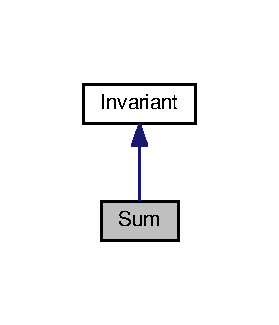
\includegraphics[width=134pt]{class_sum__inherit__graph}
\end{center}
\end{figure}


Collaboration diagram for Sum\-:\nopagebreak
\begin{figure}[H]
\begin{center}
\leavevmode
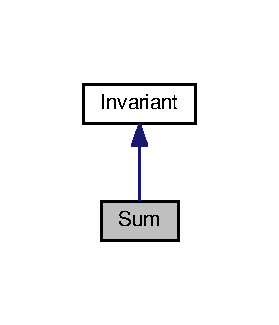
\includegraphics[width=134pt]{class_sum__coll__graph}
\end{center}
\end{figure}
\subsection*{Public Member Functions}
\begin{DoxyCompactItemize}
\item 
\hyperlink{class_sum_a040422e1db02842bf2c81575d90cceec}{Sum} (std\-::vector$<$ \hyperlink{class_integer_variable}{Integer\-Variable} $\ast$ $>$ \&vars, std\-::vector$<$ int $>$ \&c)
\item 
\hyperlink{class_sum_a48e47cd10ccf9c06deb6f675f325e1f4}{Sum} (std\-::vector$<$ \hyperlink{class_integer_variable}{Integer\-Variable} $\ast$ $>$ \&vars, std\-::unordered\-\_\-map$<$ int, \hyperlink{_constants_8hpp_a08c47c54ab9fb1545c341ec853cc2278}{coef\-Type} $>$ \&map)
\begin{DoxyCompactList}\small\item\em Construct that copies a Coefficient map. Size can be different when this sum contains invariants. \end{DoxyCompactList}\item 
\hyperlink{class_sum_a3460bcef17644813aa7200d8dd6b1750}{Sum} (const \hyperlink{class_sum}{Sum} \&a)
\item 
\hyperlink{class_sum_a9481fc530cb81210b25ecb2530d25773}{$\sim$\-Sum} ()
\item 
\hyperlink{class_sum}{Sum} \& \hyperlink{class_sum_a6a0a9edc7fc997187cec32eba22f087e}{operator=} (const \hyperlink{class_sum}{Sum} \&a)
\item 
int \hyperlink{class_sum_a6b0ada7dc577609e3140a8695155f280}{calculate\-Delta\-Value} ()
\item 
void \hyperlink{class_sum_aa66687e018c67ebedcabd69750374e2d}{add\-Change} (int variable\-Number, int change\-In\-Value)
\item 
bool \hyperlink{class_sum_a1adcbbefeb5f25445563fada563d4fa1}{test} ()
\begin{DoxyCompactList}\small\item\em update current\-Value by adding current\-Value$\ast$coeff of all variables and invariants \end{DoxyCompactList}\end{DoxyCompactItemize}
\subsection*{Protected Attributes}
\begin{DoxyCompactItemize}
\item 
std\-::vector$<$ int $>$ \hyperlink{class_sum_a10e9f89fdcf0f674e0280629144b3f92}{Variable\-Change}
\end{DoxyCompactItemize}


\subsection{Constructor \& Destructor Documentation}
\hypertarget{class_sum_a040422e1db02842bf2c81575d90cceec}{\index{Sum@{Sum}!Sum@{Sum}}
\index{Sum@{Sum}!Sum@{Sum}}
\subsubsection[{Sum}]{\setlength{\rightskip}{0pt plus 5cm}Sum\-::\-Sum (
\begin{DoxyParamCaption}
\item[{std\-::vector$<$ {\bf Integer\-Variable} $\ast$ $>$ \&}]{vars, }
\item[{std\-::vector$<$ int $>$ \&}]{c}
\end{DoxyParamCaption}
)}}\label{class_sum_a040422e1db02842bf2c81575d90cceec}
\hypertarget{class_sum_a48e47cd10ccf9c06deb6f675f325e1f4}{\index{Sum@{Sum}!Sum@{Sum}}
\index{Sum@{Sum}!Sum@{Sum}}
\subsubsection[{Sum}]{\setlength{\rightskip}{0pt plus 5cm}Sum\-::\-Sum (
\begin{DoxyParamCaption}
\item[{std\-::vector$<$ {\bf Integer\-Variable} $\ast$ $>$ \&}]{vars, }
\item[{std\-::unordered\-\_\-map$<$ int, {\bf coef\-Type} $>$ \&}]{map}
\end{DoxyParamCaption}
)}}\label{class_sum_a48e47cd10ccf9c06deb6f675f325e1f4}


Construct that copies a Coefficient map. Size can be different when this sum contains invariants. 

\hypertarget{class_sum_a3460bcef17644813aa7200d8dd6b1750}{\index{Sum@{Sum}!Sum@{Sum}}
\index{Sum@{Sum}!Sum@{Sum}}
\subsubsection[{Sum}]{\setlength{\rightskip}{0pt plus 5cm}Sum\-::\-Sum (
\begin{DoxyParamCaption}
\item[{const {\bf Sum} \&}]{a}
\end{DoxyParamCaption}
)}}\label{class_sum_a3460bcef17644813aa7200d8dd6b1750}
\hypertarget{class_sum_a9481fc530cb81210b25ecb2530d25773}{\index{Sum@{Sum}!$\sim$\-Sum@{$\sim$\-Sum}}
\index{$\sim$\-Sum@{$\sim$\-Sum}!Sum@{Sum}}
\subsubsection[{$\sim$\-Sum}]{\setlength{\rightskip}{0pt plus 5cm}Sum\-::$\sim$\-Sum (
\begin{DoxyParamCaption}
{}
\end{DoxyParamCaption}
)}}\label{class_sum_a9481fc530cb81210b25ecb2530d25773}


\subsection{Member Function Documentation}
\hypertarget{class_sum_aa66687e018c67ebedcabd69750374e2d}{\index{Sum@{Sum}!add\-Change@{add\-Change}}
\index{add\-Change@{add\-Change}!Sum@{Sum}}
\subsubsection[{add\-Change}]{\setlength{\rightskip}{0pt plus 5cm}void Sum\-::add\-Change (
\begin{DoxyParamCaption}
\item[{int}]{variable\-Number, }
\item[{int}]{change\-In\-Value}
\end{DoxyParamCaption}
)\hspace{0.3cm}{\ttfamily [virtual]}}}\label{class_sum_aa66687e018c67ebedcabd69750374e2d}


Reimplemented from \hyperlink{class_invariant_a76632dc09fe3537f159230620406fdff}{Invariant}.

\hypertarget{class_sum_a6b0ada7dc577609e3140a8695155f280}{\index{Sum@{Sum}!calculate\-Delta\-Value@{calculate\-Delta\-Value}}
\index{calculate\-Delta\-Value@{calculate\-Delta\-Value}!Sum@{Sum}}
\subsubsection[{calculate\-Delta\-Value}]{\setlength{\rightskip}{0pt plus 5cm}int Sum\-::calculate\-Delta\-Value (
\begin{DoxyParamCaption}
{}
\end{DoxyParamCaption}
)\hspace{0.3cm}{\ttfamily [virtual]}}}\label{class_sum_a6b0ada7dc577609e3140a8695155f280}


Reimplemented from \hyperlink{class_invariant_a4797e907bd38e68769962949b453ae7a}{Invariant}.

\hypertarget{class_sum_a6a0a9edc7fc997187cec32eba22f087e}{\index{Sum@{Sum}!operator=@{operator=}}
\index{operator=@{operator=}!Sum@{Sum}}
\subsubsection[{operator=}]{\setlength{\rightskip}{0pt plus 5cm}{\bf Sum}\& Sum\-::operator= (
\begin{DoxyParamCaption}
\item[{const {\bf Sum} \&}]{a}
\end{DoxyParamCaption}
)}}\label{class_sum_a6a0a9edc7fc997187cec32eba22f087e}
\hypertarget{class_sum_a1adcbbefeb5f25445563fada563d4fa1}{\index{Sum@{Sum}!test@{test}}
\index{test@{test}!Sum@{Sum}}
\subsubsection[{test}]{\setlength{\rightskip}{0pt plus 5cm}bool Sum\-::test (
\begin{DoxyParamCaption}
{}
\end{DoxyParamCaption}
)\hspace{0.3cm}{\ttfamily [virtual]}}}\label{class_sum_a1adcbbefeb5f25445563fada563d4fa1}


update current\-Value by adding current\-Value$\ast$coeff of all variables and invariants 



Reimplemented from \hyperlink{class_invariant_ab3fd6fa5c99ed9854756347a439e0fd9}{Invariant}.



\subsection{Member Data Documentation}
\hypertarget{class_sum_a10e9f89fdcf0f674e0280629144b3f92}{\index{Sum@{Sum}!Variable\-Change@{Variable\-Change}}
\index{Variable\-Change@{Variable\-Change}!Sum@{Sum}}
\subsubsection[{Variable\-Change}]{\setlength{\rightskip}{0pt plus 5cm}std\-::vector$<$int$>$ Sum\-::\-Variable\-Change\hspace{0.3cm}{\ttfamily [protected]}}}\label{class_sum_a10e9f89fdcf0f674e0280629144b3f92}


The documentation for this class was generated from the following files\-:\begin{DoxyCompactItemize}
\item 
\hyperlink{_sum_8hpp}{Sum.\-hpp}\item 
\hyperlink{_sum_8cpp}{Sum.\-cpp}\end{DoxyCompactItemize}

\hypertarget{class_value_change_move}{\section{Value\-Change\-Move Class Reference}
\label{class_value_change_move}\index{Value\-Change\-Move@{Value\-Change\-Move}}
}


{\ttfamily \#include $<$Value\-Change\-Move.\-hpp$>$}



Inheritance diagram for Value\-Change\-Move\-:\nopagebreak
\begin{figure}[H]
\begin{center}
\leavevmode
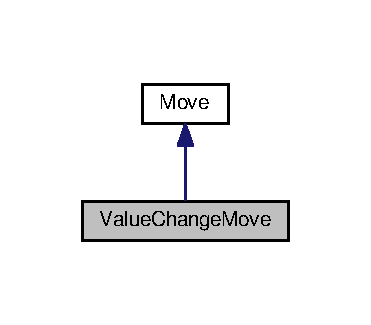
\includegraphics[width=178pt]{class_value_change_move__inherit__graph}
\end{center}
\end{figure}


Collaboration diagram for Value\-Change\-Move\-:\nopagebreak
\begin{figure}[H]
\begin{center}
\leavevmode
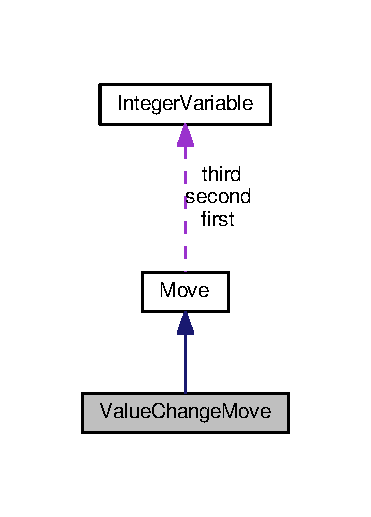
\includegraphics[width=178pt]{class_value_change_move__coll__graph}
\end{center}
\end{figure}
\subsection*{Public Member Functions}
\begin{DoxyCompactItemize}
\item 
\hyperlink{class_value_change_move_acc99c9e1bb0ee0de467eccad1f6a5b82}{Value\-Change\-Move} (\hyperlink{class_integer_variable}{Integer\-Variable} $\ast$iv, int new\-Value)
\item 
\hyperlink{class_value_change_move_aece5e02665f3c8b99de2398f3f5f1908}{Value\-Change\-Move} (const \hyperlink{class_value_change_move}{Value\-Change\-Move} \&orig)
\item 
\hyperlink{class_value_change_move_a3b39bee115ac86227411c76723715907}{$\sim$\-Value\-Change\-Move} ()
\item 
\hyperlink{class_value_change_move}{Value\-Change\-Move} \& \hyperlink{class_value_change_move_ae6242fe996cf5df1de8a65db5921f397}{operator=} (const \hyperlink{class_value_change_move}{Value\-Change\-Move} \&a)
\end{DoxyCompactItemize}
\subsection*{Additional Inherited Members}


\subsection{Constructor \& Destructor Documentation}
\hypertarget{class_value_change_move_acc99c9e1bb0ee0de467eccad1f6a5b82}{\index{Value\-Change\-Move@{Value\-Change\-Move}!Value\-Change\-Move@{Value\-Change\-Move}}
\index{Value\-Change\-Move@{Value\-Change\-Move}!ValueChangeMove@{Value\-Change\-Move}}
\subsubsection[{Value\-Change\-Move}]{\setlength{\rightskip}{0pt plus 5cm}Value\-Change\-Move\-::\-Value\-Change\-Move (
\begin{DoxyParamCaption}
\item[{{\bf Integer\-Variable} $\ast$}]{iv, }
\item[{int}]{new\-Value}
\end{DoxyParamCaption}
)}}\label{class_value_change_move_acc99c9e1bb0ee0de467eccad1f6a5b82}
\hypertarget{class_value_change_move_aece5e02665f3c8b99de2398f3f5f1908}{\index{Value\-Change\-Move@{Value\-Change\-Move}!Value\-Change\-Move@{Value\-Change\-Move}}
\index{Value\-Change\-Move@{Value\-Change\-Move}!ValueChangeMove@{Value\-Change\-Move}}
\subsubsection[{Value\-Change\-Move}]{\setlength{\rightskip}{0pt plus 5cm}Value\-Change\-Move\-::\-Value\-Change\-Move (
\begin{DoxyParamCaption}
\item[{const {\bf Value\-Change\-Move} \&}]{orig}
\end{DoxyParamCaption}
)}}\label{class_value_change_move_aece5e02665f3c8b99de2398f3f5f1908}
\hypertarget{class_value_change_move_a3b39bee115ac86227411c76723715907}{\index{Value\-Change\-Move@{Value\-Change\-Move}!$\sim$\-Value\-Change\-Move@{$\sim$\-Value\-Change\-Move}}
\index{$\sim$\-Value\-Change\-Move@{$\sim$\-Value\-Change\-Move}!ValueChangeMove@{Value\-Change\-Move}}
\subsubsection[{$\sim$\-Value\-Change\-Move}]{\setlength{\rightskip}{0pt plus 5cm}Value\-Change\-Move\-::$\sim$\-Value\-Change\-Move (
\begin{DoxyParamCaption}
{}
\end{DoxyParamCaption}
)}}\label{class_value_change_move_a3b39bee115ac86227411c76723715907}


\subsection{Member Function Documentation}
\hypertarget{class_value_change_move_ae6242fe996cf5df1de8a65db5921f397}{\index{Value\-Change\-Move@{Value\-Change\-Move}!operator=@{operator=}}
\index{operator=@{operator=}!ValueChangeMove@{Value\-Change\-Move}}
\subsubsection[{operator=}]{\setlength{\rightskip}{0pt plus 5cm}{\bf Value\-Change\-Move} \& Value\-Change\-Move\-::operator= (
\begin{DoxyParamCaption}
\item[{const {\bf Value\-Change\-Move} \&}]{a}
\end{DoxyParamCaption}
)}}\label{class_value_change_move_ae6242fe996cf5df1de8a65db5921f397}


The documentation for this class was generated from the following files\-:\begin{DoxyCompactItemize}
\item 
\hyperlink{_value_change_move_8hpp}{Value\-Change\-Move.\-hpp}\item 
\hyperlink{_value_change_move_8cpp}{Value\-Change\-Move.\-cpp}\end{DoxyCompactItemize}

\hypertarget{structvar}{\section{var Struct Reference}
\label{structvar}\index{var@{var}}
}


{\ttfamily \#include $<$B\-P\-\_\-\-Data.\-hpp$>$}



Inheritance diagram for var\-:\nopagebreak
\begin{figure}[H]
\begin{center}
\leavevmode
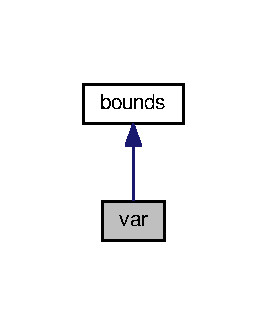
\includegraphics[width=128pt]{structvar__inherit__graph}
\end{center}
\end{figure}


Collaboration diagram for var\-:\nopagebreak
\begin{figure}[H]
\begin{center}
\leavevmode
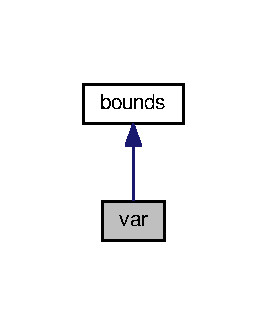
\includegraphics[width=128pt]{structvar__coll__graph}
\end{center}
\end{figure}
\subsection*{Public Member Functions}
\begin{DoxyCompactItemize}
\item 
\hyperlink{structvar_ac7d2944f98e9772ab540050ae22fe9d1}{$\sim$var} ()
\end{DoxyCompactItemize}
\subsection*{Public Attributes}
\begin{DoxyCompactItemize}
\item 
double \hyperlink{structvar_a3c9ce9241d544abb8301a79b4f86302a}{objcoeff}
\item 
int \hyperlink{structvar_a11eae9366edca3b0b8b400c090654124}{kind}
\item 
bool \hyperlink{structvar_aa5808e92bc45bfada22c08a76f4fc8f5}{bin}
\end{DoxyCompactItemize}


\subsection{Constructor \& Destructor Documentation}
\hypertarget{structvar_ac7d2944f98e9772ab540050ae22fe9d1}{\index{var@{var}!$\sim$var@{$\sim$var}}
\index{$\sim$var@{$\sim$var}!var@{var}}
\subsubsection[{$\sim$var}]{\setlength{\rightskip}{0pt plus 5cm}var\-::$\sim$var (
\begin{DoxyParamCaption}
{}
\end{DoxyParamCaption}
)\hspace{0.3cm}{\ttfamily [inline]}}}\label{structvar_ac7d2944f98e9772ab540050ae22fe9d1}


\subsection{Member Data Documentation}
\hypertarget{structvar_aa5808e92bc45bfada22c08a76f4fc8f5}{\index{var@{var}!bin@{bin}}
\index{bin@{bin}!var@{var}}
\subsubsection[{bin}]{\setlength{\rightskip}{0pt plus 5cm}bool var\-::bin}}\label{structvar_aa5808e92bc45bfada22c08a76f4fc8f5}
\hypertarget{structvar_a11eae9366edca3b0b8b400c090654124}{\index{var@{var}!kind@{kind}}
\index{kind@{kind}!var@{var}}
\subsubsection[{kind}]{\setlength{\rightskip}{0pt plus 5cm}int var\-::kind}}\label{structvar_a11eae9366edca3b0b8b400c090654124}
\hypertarget{structvar_a3c9ce9241d544abb8301a79b4f86302a}{\index{var@{var}!objcoeff@{objcoeff}}
\index{objcoeff@{objcoeff}!var@{var}}
\subsubsection[{objcoeff}]{\setlength{\rightskip}{0pt plus 5cm}double var\-::objcoeff}}\label{structvar_a3c9ce9241d544abb8301a79b4f86302a}


The documentation for this struct was generated from the following file\-:\begin{DoxyCompactItemize}
\item 
\hyperlink{_b_p___data_8hpp}{B\-P\-\_\-\-Data.\-hpp}\end{DoxyCompactItemize}

\chapter{File Documentation}
\hypertarget{_b_p___data_8cpp}{\section{B\-P\-\_\-\-Data.\-cpp File Reference}
\label{_b_p___data_8cpp}\index{B\-P\-\_\-\-Data.\-cpp@{B\-P\-\_\-\-Data.\-cpp}}
}
{\ttfamily \#include \char`\"{}B\-P\-\_\-\-Data.\-hpp\char`\"{}}\\*
Include dependency graph for B\-P\-\_\-\-Data.\-cpp\-:\nopagebreak
\begin{figure}[H]
\begin{center}
\leavevmode
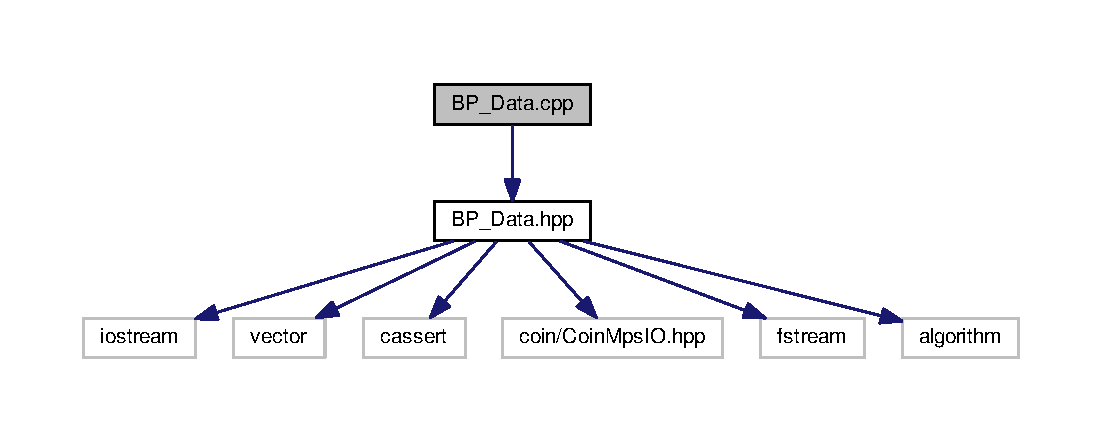
\includegraphics[width=350pt]{_b_p___data_8cpp__incl}
\end{center}
\end{figure}
\subsection*{Functions}
\begin{DoxyCompactItemize}
\item 
ostream \& \hyperlink{_b_p___data_8cpp_a1d1741e17f725be51640a6d881d768fa}{operator$<$$<$} (ostream \&os, const \hyperlink{class_b_p___output}{B\-P\-\_\-\-Output} \&out)
\item 
istream \& \hyperlink{_b_p___data_8cpp_a401e305330b684d15b38d6a6a0bfb25f}{operator$>$$>$} (istream \&is, \hyperlink{class_b_p___output}{B\-P\-\_\-\-Output} \&out)
\end{DoxyCompactItemize}


\subsection{Function Documentation}
\hypertarget{_b_p___data_8cpp_a1d1741e17f725be51640a6d881d768fa}{\index{B\-P\-\_\-\-Data.\-cpp@{B\-P\-\_\-\-Data.\-cpp}!operator$<$$<$@{operator$<$$<$}}
\index{operator$<$$<$@{operator$<$$<$}!BP_Data.cpp@{B\-P\-\_\-\-Data.\-cpp}}
\subsubsection[{operator$<$$<$}]{\setlength{\rightskip}{0pt plus 5cm}ostream\& operator$<$$<$ (
\begin{DoxyParamCaption}
\item[{ostream \&}]{os, }
\item[{const {\bf B\-P\-\_\-\-Output} \&}]{out}
\end{DoxyParamCaption}
)}}\label{_b_p___data_8cpp_a1d1741e17f725be51640a6d881d768fa}
\hypertarget{_b_p___data_8cpp_a401e305330b684d15b38d6a6a0bfb25f}{\index{B\-P\-\_\-\-Data.\-cpp@{B\-P\-\_\-\-Data.\-cpp}!operator$>$$>$@{operator$>$$>$}}
\index{operator$>$$>$@{operator$>$$>$}!BP_Data.cpp@{B\-P\-\_\-\-Data.\-cpp}}
\subsubsection[{operator$>$$>$}]{\setlength{\rightskip}{0pt plus 5cm}istream\& operator$>$$>$ (
\begin{DoxyParamCaption}
\item[{istream \&}]{is, }
\item[{{\bf B\-P\-\_\-\-Output} \&}]{out}
\end{DoxyParamCaption}
)}}\label{_b_p___data_8cpp_a401e305330b684d15b38d6a6a0bfb25f}

\hypertarget{_b_p___data_8hpp}{\section{B\-P\-\_\-\-Data.\-hpp File Reference}
\label{_b_p___data_8hpp}\index{B\-P\-\_\-\-Data.\-hpp@{B\-P\-\_\-\-Data.\-hpp}}
}
{\ttfamily \#include $<$iostream$>$}\\*
{\ttfamily \#include $<$vector$>$}\\*
{\ttfamily \#include $<$cassert$>$}\\*
{\ttfamily \#include \char`\"{}coin/\-Coin\-Mps\-I\-O.\-hpp\char`\"{}}\\*
{\ttfamily \#include $<$fstream$>$}\\*
{\ttfamily \#include $<$algorithm$>$}\\*
Include dependency graph for B\-P\-\_\-\-Data.\-hpp\-:\nopagebreak
\begin{figure}[H]
\begin{center}
\leavevmode
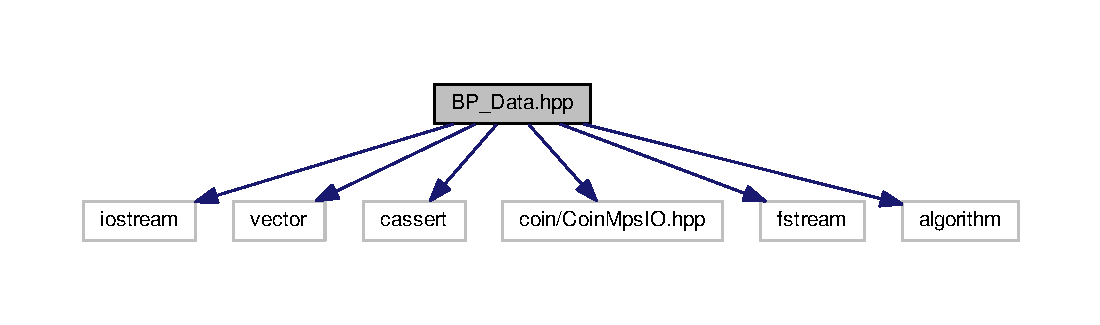
\includegraphics[width=350pt]{_b_p___data_8hpp__incl}
\end{center}
\end{figure}
This graph shows which files directly or indirectly include this file\-:\nopagebreak
\begin{figure}[H]
\begin{center}
\leavevmode
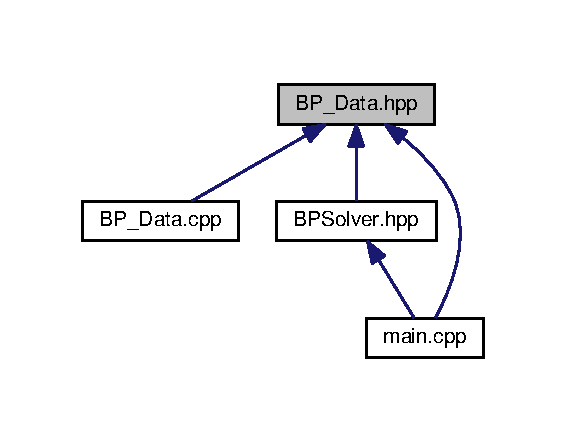
\includegraphics[width=271pt]{_b_p___data_8hpp__dep__incl}
\end{center}
\end{figure}
\subsection*{Classes}
\begin{DoxyCompactItemize}
\item 
struct \hyperlink{structelem}{elem}
\item 
struct \hyperlink{structbounds}{bounds}
\item 
struct \hyperlink{structvar}{var}
\item 
class \hyperlink{class_b_p___input}{B\-P\-\_\-\-Input}
\item 
class \hyperlink{class_b_p___output}{B\-P\-\_\-\-Output}
\end{DoxyCompactItemize}
\subsection*{Macros}
\begin{DoxyCompactItemize}
\item 
\#define \hyperlink{_b_p___data_8hpp_aef41e8aaf4c60819b30faf396cdf4978}{D\-E\-B\-U\-G}(X)~X
\end{DoxyCompactItemize}


\subsection{Macro Definition Documentation}
\hypertarget{_b_p___data_8hpp_aef41e8aaf4c60819b30faf396cdf4978}{\index{B\-P\-\_\-\-Data.\-hpp@{B\-P\-\_\-\-Data.\-hpp}!D\-E\-B\-U\-G@{D\-E\-B\-U\-G}}
\index{D\-E\-B\-U\-G@{D\-E\-B\-U\-G}!BP_Data.hpp@{B\-P\-\_\-\-Data.\-hpp}}
\subsubsection[{D\-E\-B\-U\-G}]{\setlength{\rightskip}{0pt plus 5cm}\#define D\-E\-B\-U\-G(
\begin{DoxyParamCaption}
\item[{}]{X}
\end{DoxyParamCaption}
)~X}}\label{_b_p___data_8hpp_aef41e8aaf4c60819b30faf396cdf4978}

\hypertarget{_b_p_solver_8hpp}{\section{B\-P\-Solver.\-hpp File Reference}
\label{_b_p_solver_8hpp}\index{B\-P\-Solver.\-hpp@{B\-P\-Solver.\-hpp}}
}
{\ttfamily \#include \char`\"{}B\-P\-\_\-\-Data.\-hpp\char`\"{}}\\*
{\ttfamily \#include $<$cmath$>$}\\*
{\ttfamily \#include $<$algorithm$>$}\\*
{\ttfamily \#include \char`\"{}General\-Solver.\-hpp\char`\"{}}\\*
{\ttfamily \#include \char`\"{}Integer\-Variable.\-hpp\char`\"{}}\\*
Include dependency graph for B\-P\-Solver.\-hpp\-:\nopagebreak
\begin{figure}[H]
\begin{center}
\leavevmode
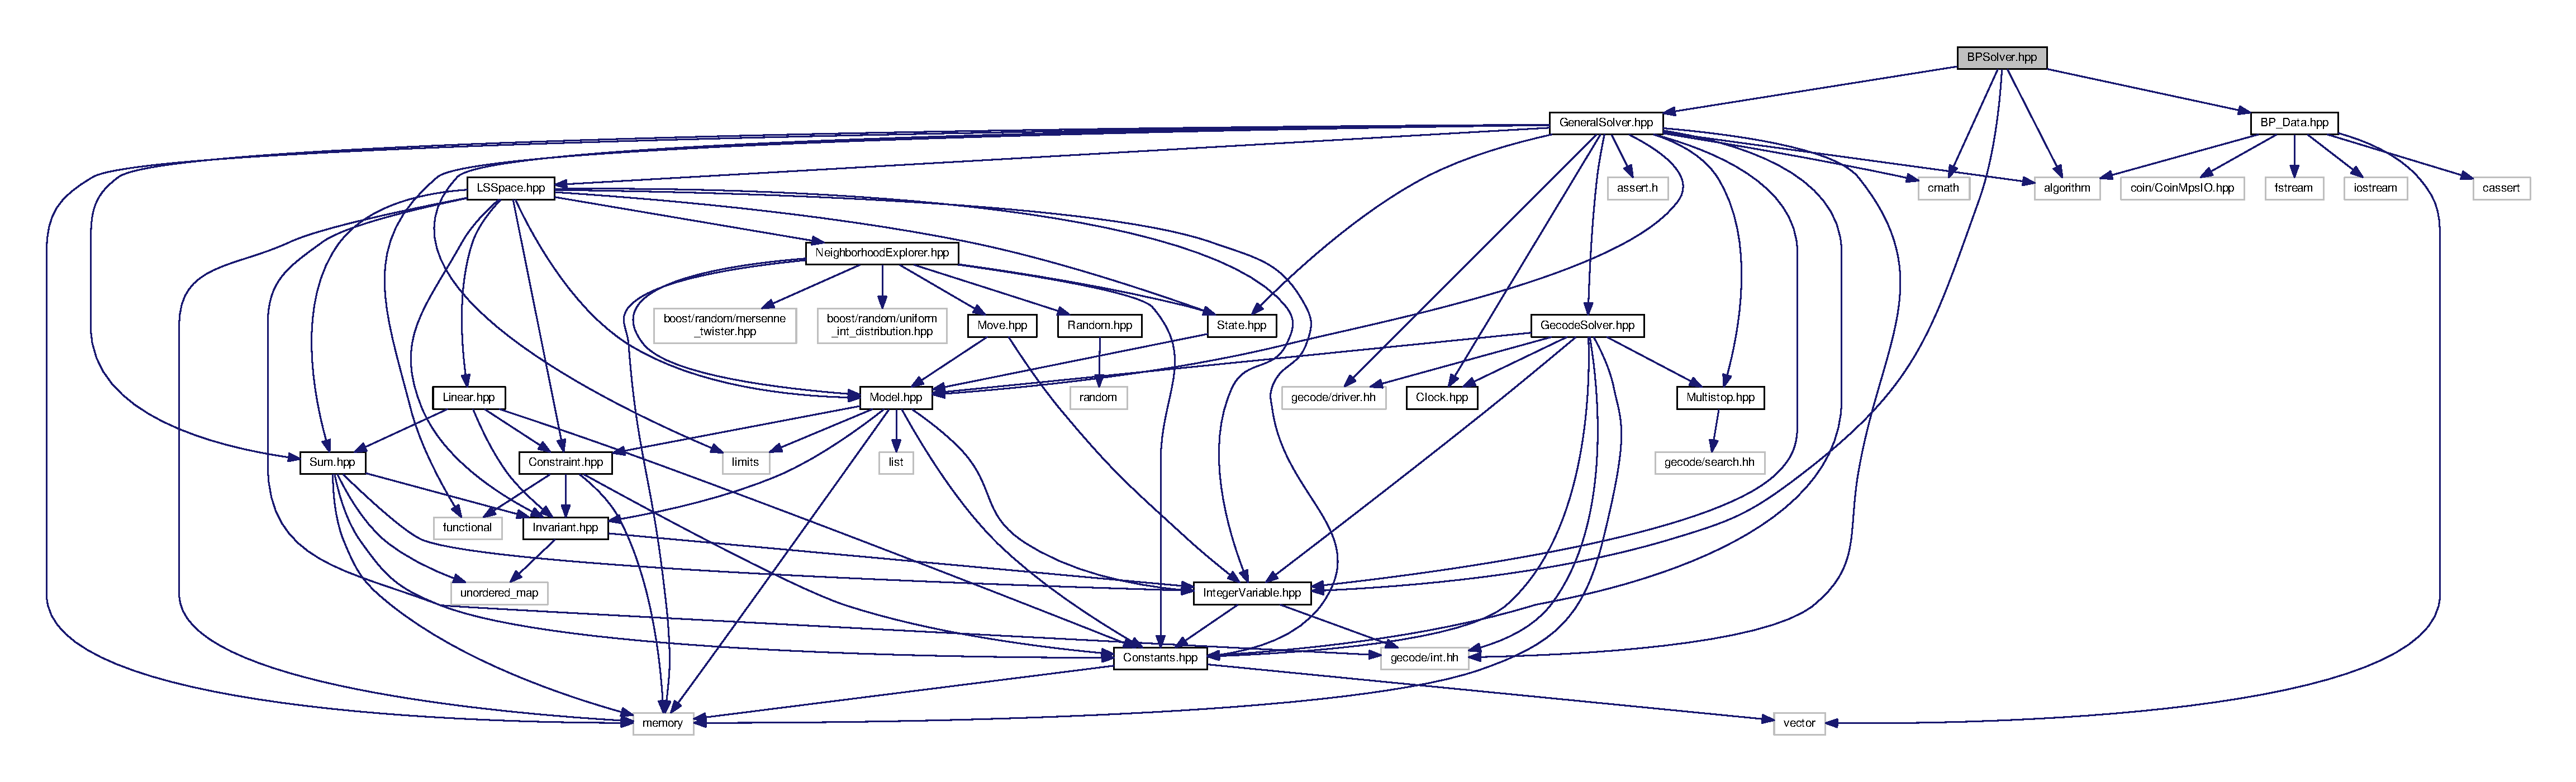
\includegraphics[width=350pt]{_b_p_solver_8hpp__incl}
\end{center}
\end{figure}
This graph shows which files directly or indirectly include this file\-:\nopagebreak
\begin{figure}[H]
\begin{center}
\leavevmode
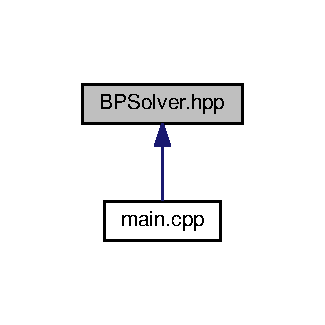
\includegraphics[width=156pt]{_b_p_solver_8hpp__dep__incl}
\end{center}
\end{figure}
\subsection*{Classes}
\begin{DoxyCompactItemize}
\item 
class \hyperlink{class_b_p_solver}{B\-P\-Solver}
\end{DoxyCompactItemize}

\hypertarget{_clock_8cpp}{\section{Clock.\-cpp File Reference}
\label{_clock_8cpp}\index{Clock.\-cpp@{Clock.\-cpp}}
}
{\ttfamily \#include \char`\"{}Clock.\-hpp\char`\"{}}\\*
Include dependency graph for Clock.\-cpp\-:\nopagebreak
\begin{figure}[H]
\begin{center}
\leavevmode
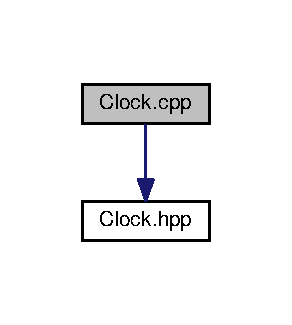
\includegraphics[width=140pt]{_clock_8cpp__incl}
\end{center}
\end{figure}

\hypertarget{_clock_8hpp}{\section{Clock.\-hpp File Reference}
\label{_clock_8hpp}\index{Clock.\-hpp@{Clock.\-hpp}}
}
This graph shows which files directly or indirectly include this file\-:
\nopagebreak
\begin{figure}[H]
\begin{center}
\leavevmode
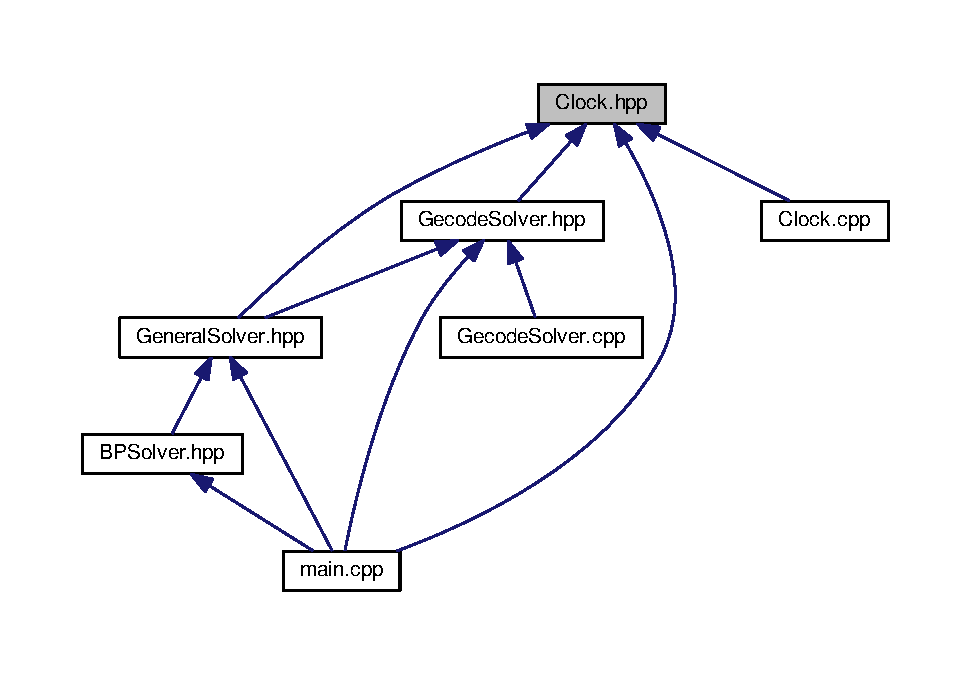
\includegraphics[width=350pt]{_clock_8hpp__dep__incl}
\end{center}
\end{figure}
\subsection*{Classes}
\begin{DoxyCompactItemize}
\item 
class \hyperlink{class_clock}{Clock}
\end{DoxyCompactItemize}

\hypertarget{_constants_8hpp}{\section{Constants.\-hpp File Reference}
\label{_constants_8hpp}\index{Constants.\-hpp@{Constants.\-hpp}}
}
{\ttfamily \#include $<$memory$>$}\\*
{\ttfamily \#include $<$vector$>$}\\*
Include dependency graph for Constants.\-hpp\-:\nopagebreak
\begin{figure}[H]
\begin{center}
\leavevmode
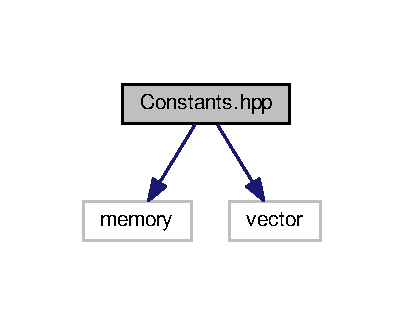
\includegraphics[width=193pt]{_constants_8hpp__incl}
\end{center}
\end{figure}
This graph shows which files directly or indirectly include this file\-:
\nopagebreak
\begin{figure}[H]
\begin{center}
\leavevmode
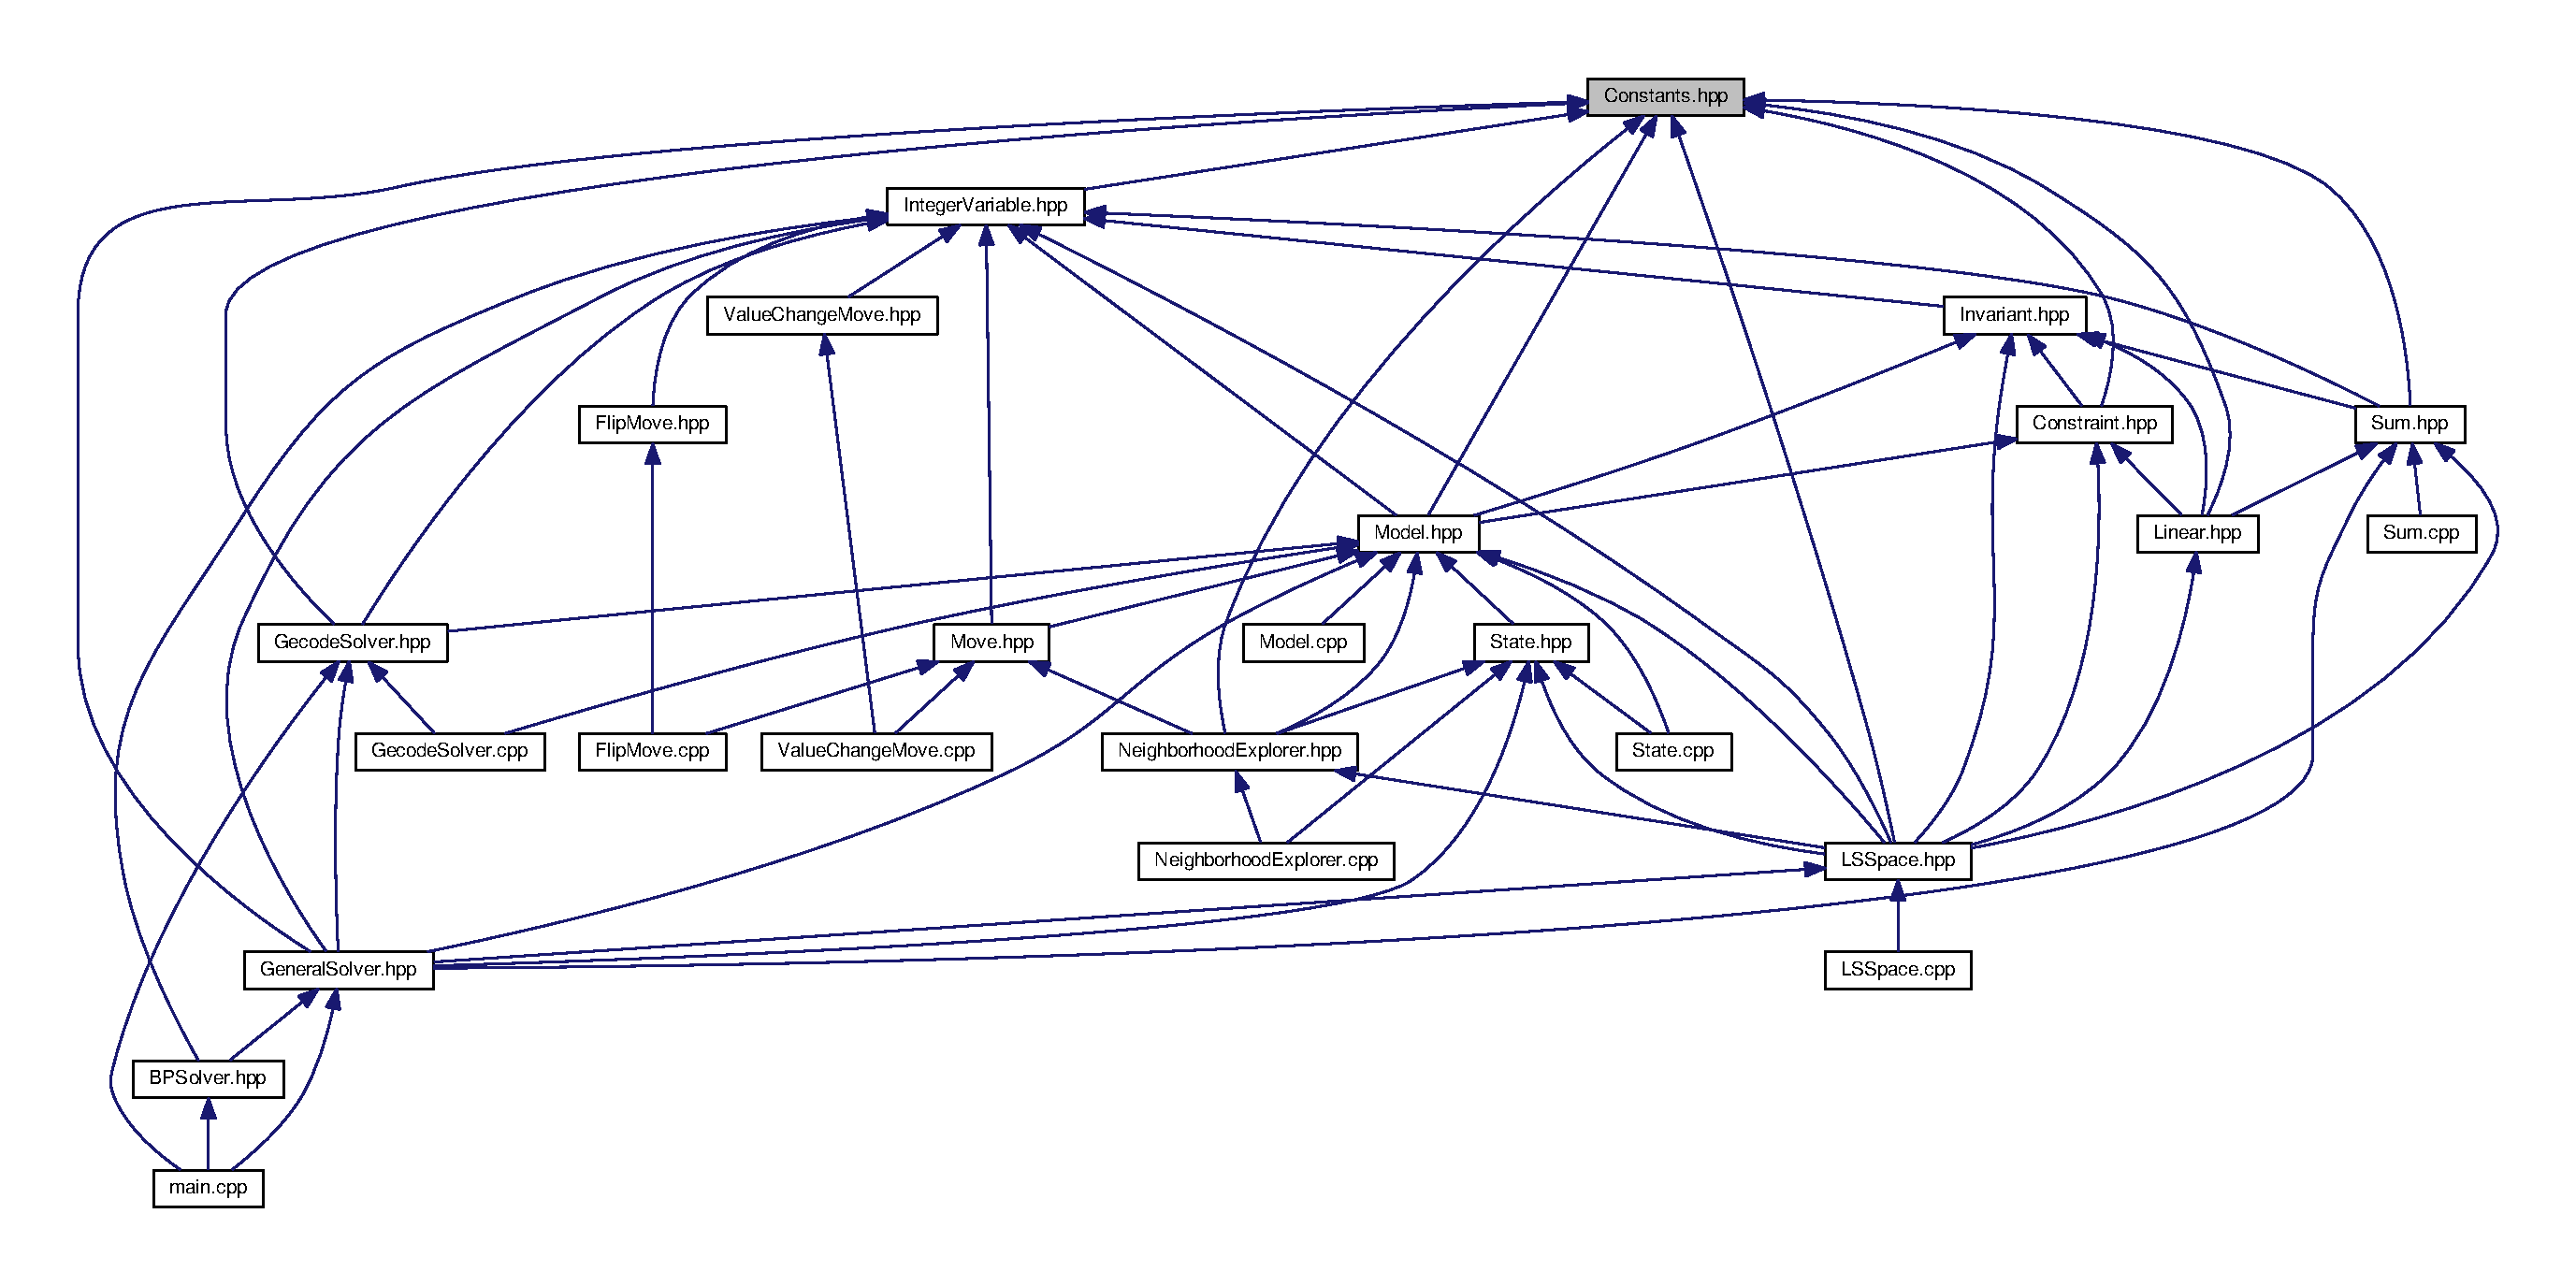
\includegraphics[width=350pt]{_constants_8hpp__dep__incl}
\end{center}
\end{figure}
\subsection*{Macros}
\begin{DoxyCompactItemize}
\item 
\#define \hyperlink{_constants_8hpp_a02c5cabeb07eb03153a81bae2256a7c4}{non\-Term}~0.\-000000000001
\item 
\#define \hyperlink{_constants_8hpp_aa9729b9af09826debfd9aa4e44005087}{weight}~100
\item 
\#define \hyperlink{_constants_8hpp_aaf5f01676b00106b4e4fa666cb9679c1}{tabulist\-L\-B}~5
\item 
\#define \hyperlink{_constants_8hpp_ad994156ac2ec126d182014973578cd7b}{tabulist\-U\-B}~20
\item 
\#define \hyperlink{_constants_8hpp_ad55cedde79cf370797a15c166e2c33da}{max\-Iter}~200000000
\item 
\#define \hyperlink{_constants_8hpp_a8f7b3ffb44731a2241253c6da1056db7}{ini\-Trails}~20
\item 
\#define \hyperlink{_constants_8hpp_ace46574cbdb946dee558ca28994410ca}{max\-Moves}~600
\item 
\#define \hyperlink{_constants_8hpp_a0bea41a2c6b9e3c1d20d143f11d474a9}{R\-A\-N\-D\-O\-M\-S\-E\-E\-D}~1337
\item 
\#define \hyperlink{_constants_8hpp_a8b43bafee90b30676faae508c21cb8d7}{P\-R\-I\-N\-T}~T\-R\-U\-E
\item 
\#define \hyperlink{_constants_8hpp_a322565ccf348d13e4d3de13af771e5fc}{debug}~std\-::cout $<$$<$ \-\_\-\-\_\-\-F\-I\-L\-E\-\_\-\-\_\- $<$$<$ \char`\"{} \char`\"{} $<$$<$ \-\_\-\-\_\-\-F\-U\-N\-C\-T\-I\-O\-N\-\_\-\-\_\- $<$$<$ \char`\"{} \char`\"{} $<$$<$ \-\_\-\-\_\-\-L\-I\-N\-E\-\_\-\-\_\- $<$$<$ std\-::endl;
\item 
\#define \hyperlink{_constants_8hpp_abaab8d42f075ee8ddc9b70951d3fd6cd}{E\-Q}~0
\item 
\#define \hyperlink{_constants_8hpp_a00d06291a8099ffe9b6e420156965050}{L\-Q}~1
\item 
\#define \hyperlink{_constants_8hpp_a6577e6b57bcfaf2e09450cb278a072e3}{G\-Q}~3
\item 
\#define \hyperlink{_constants_8hpp_a656da95f9680f14093be09a52ab6752f}{G\-R}~4
\item 
\#define \hyperlink{_constants_8hpp_aa4d6abc7b58eb11e517993df83b7f0f7}{L\-E}~2
\item 
\#define \hyperlink{_constants_8hpp_adbde5b9da0fc01ad88668b5f24c2c256}{O\-B\-J}~0
\item 
\#define \hyperlink{_constants_8hpp_a4d14a79c82f3f831303e38487811eda4}{H\-A\-R\-D}~1
\item 
\#define \hyperlink{_constants_8hpp_a1b44ecf82561bec987fa3c07632335a4}{S\-O\-F\-T}~2
\item 
\#define \hyperlink{_constants_8hpp_a6913edbcb0c881679fd7dd121c10af3e}{F\-L\-I\-P}~1
\item 
\#define \hyperlink{_constants_8hpp_aac9b57651bcead0a7564efe6460e5310}{S\-W\-A\-P}~2
\item 
\#define \hyperlink{_constants_8hpp_a0cce99f95c35cfa782d6b6a83df08fa0}{V\-A\-L\-U\-E\-C\-H\-A\-N\-G\-E}~3
\item 
\#define \hyperlink{_constants_8hpp_ac645eb9a88619ee6f5e14c557ab8ef62}{L\-I\-N\-E\-A\-R}~1
\item 
\#define \hyperlink{_constants_8hpp_a1319745524dbd8748dba95bb12b19f19}{S\-U\-M}~1
\end{DoxyCompactItemize}
\subsection*{Typedefs}
\begin{DoxyCompactItemize}
\item 
typedef double \hyperlink{_constants_8hpp_a08c47c54ab9fb1545c341ec853cc2278}{coef\-Type}
\item 
typedef std\-::shared\-\_\-ptr\\*
$<$ \hyperlink{class_constraint}{Constraint} $>$ \hyperlink{_constants_8hpp_ab3a9f5ca3242dd173f530bb9f68fc611}{constraint}
\item 
typedef std\-::vector\\*
$<$ \hyperlink{class_integer_variable}{Integer\-Variable} $\ast$ $>$ \hyperlink{_constants_8hpp_a30d6ea0a65b32e8b74cc6126cea9852e}{variable\-Container}
\item 
typedef std\-::vector$<$ \hyperlink{_constants_8hpp_ab3a9f5ca3242dd173f530bb9f68fc611}{constraint} $>$ \hyperlink{_constants_8hpp_a02baa5ed1a26d5d8a8c4adb2d0e59a57}{Variable\-In\-Constraints}
\item 
typedef std\-::shared\-\_\-ptr\\*
$<$ \hyperlink{class_invariant}{Invariant} $>$ \hyperlink{_constants_8hpp_ac9b562f250a09412c017b68185321eba}{invariant}
\item 
typedef std\-::vector$<$ \hyperlink{_constants_8hpp_ac9b562f250a09412c017b68185321eba}{invariant} $>$ \hyperlink{_constants_8hpp_a5ea9d0c2efe357d2a7f5bcd80cdf179a}{Invariant\-Container}
\item 
typedef \hyperlink{_constants_8hpp_a5ea9d0c2efe357d2a7f5bcd80cdf179a}{Invariant\-Container} \hyperlink{_constants_8hpp_a318698c81469739a632fe21db9b9eb3b}{update\-Vector}
\item 
typedef std\-::shared\-\_\-ptr\\*
$<$ \hyperlink{class_invariant}{Invariant} $>$ \hyperlink{_constants_8hpp_a1c0fa2df7430fc28b51f047f98434f6c}{update\-Type}
\item 
typedef std\-::shared\-\_\-ptr\\*
$<$ std\-::vector$<$ \hyperlink{_constants_8hpp_ab3a9f5ca3242dd173f530bb9f68fc611}{constraint} $>$ $>$ \hyperlink{_constants_8hpp_a44699d451ee649f131b1b72451070aa0}{constraint\-Container}
\item 
typedef std\-::vector\\*
$<$ \hyperlink{_constants_8hpp_a44699d451ee649f131b1b72451070aa0}{constraint\-Container} $>$ \hyperlink{_constants_8hpp_a9cd92c30962a3af393035610635972fa}{all\-Constraints}
\end{DoxyCompactItemize}


\subsection{Macro Definition Documentation}
\hypertarget{_constants_8hpp_a322565ccf348d13e4d3de13af771e5fc}{\index{Constants.\-hpp@{Constants.\-hpp}!debug@{debug}}
\index{debug@{debug}!Constants.hpp@{Constants.\-hpp}}
\subsubsection[{debug}]{\setlength{\rightskip}{0pt plus 5cm}\#define debug~std\-::cout $<$$<$ \-\_\-\-\_\-\-F\-I\-L\-E\-\_\-\-\_\- $<$$<$ \char`\"{} \char`\"{} $<$$<$ \-\_\-\-\_\-\-F\-U\-N\-C\-T\-I\-O\-N\-\_\-\-\_\- $<$$<$ \char`\"{} \char`\"{} $<$$<$ \-\_\-\-\_\-\-L\-I\-N\-E\-\_\-\-\_\- $<$$<$ std\-::endl;}}\label{_constants_8hpp_a322565ccf348d13e4d3de13af771e5fc}
\hypertarget{_constants_8hpp_abaab8d42f075ee8ddc9b70951d3fd6cd}{\index{Constants.\-hpp@{Constants.\-hpp}!E\-Q@{E\-Q}}
\index{E\-Q@{E\-Q}!Constants.hpp@{Constants.\-hpp}}
\subsubsection[{E\-Q}]{\setlength{\rightskip}{0pt plus 5cm}\#define E\-Q~0}}\label{_constants_8hpp_abaab8d42f075ee8ddc9b70951d3fd6cd}
\hypertarget{_constants_8hpp_a6913edbcb0c881679fd7dd121c10af3e}{\index{Constants.\-hpp@{Constants.\-hpp}!F\-L\-I\-P@{F\-L\-I\-P}}
\index{F\-L\-I\-P@{F\-L\-I\-P}!Constants.hpp@{Constants.\-hpp}}
\subsubsection[{F\-L\-I\-P}]{\setlength{\rightskip}{0pt plus 5cm}\#define F\-L\-I\-P~1}}\label{_constants_8hpp_a6913edbcb0c881679fd7dd121c10af3e}
\hypertarget{_constants_8hpp_a6577e6b57bcfaf2e09450cb278a072e3}{\index{Constants.\-hpp@{Constants.\-hpp}!G\-Q@{G\-Q}}
\index{G\-Q@{G\-Q}!Constants.hpp@{Constants.\-hpp}}
\subsubsection[{G\-Q}]{\setlength{\rightskip}{0pt plus 5cm}\#define G\-Q~3}}\label{_constants_8hpp_a6577e6b57bcfaf2e09450cb278a072e3}
\hypertarget{_constants_8hpp_a656da95f9680f14093be09a52ab6752f}{\index{Constants.\-hpp@{Constants.\-hpp}!G\-R@{G\-R}}
\index{G\-R@{G\-R}!Constants.hpp@{Constants.\-hpp}}
\subsubsection[{G\-R}]{\setlength{\rightskip}{0pt plus 5cm}\#define G\-R~4}}\label{_constants_8hpp_a656da95f9680f14093be09a52ab6752f}
\hypertarget{_constants_8hpp_a4d14a79c82f3f831303e38487811eda4}{\index{Constants.\-hpp@{Constants.\-hpp}!H\-A\-R\-D@{H\-A\-R\-D}}
\index{H\-A\-R\-D@{H\-A\-R\-D}!Constants.hpp@{Constants.\-hpp}}
\subsubsection[{H\-A\-R\-D}]{\setlength{\rightskip}{0pt plus 5cm}\#define H\-A\-R\-D~1}}\label{_constants_8hpp_a4d14a79c82f3f831303e38487811eda4}
\hypertarget{_constants_8hpp_a8f7b3ffb44731a2241253c6da1056db7}{\index{Constants.\-hpp@{Constants.\-hpp}!ini\-Trails@{ini\-Trails}}
\index{ini\-Trails@{ini\-Trails}!Constants.hpp@{Constants.\-hpp}}
\subsubsection[{ini\-Trails}]{\setlength{\rightskip}{0pt plus 5cm}\#define ini\-Trails~20}}\label{_constants_8hpp_a8f7b3ffb44731a2241253c6da1056db7}
\hypertarget{_constants_8hpp_aa4d6abc7b58eb11e517993df83b7f0f7}{\index{Constants.\-hpp@{Constants.\-hpp}!L\-E@{L\-E}}
\index{L\-E@{L\-E}!Constants.hpp@{Constants.\-hpp}}
\subsubsection[{L\-E}]{\setlength{\rightskip}{0pt plus 5cm}\#define L\-E~2}}\label{_constants_8hpp_aa4d6abc7b58eb11e517993df83b7f0f7}
\hypertarget{_constants_8hpp_ac645eb9a88619ee6f5e14c557ab8ef62}{\index{Constants.\-hpp@{Constants.\-hpp}!L\-I\-N\-E\-A\-R@{L\-I\-N\-E\-A\-R}}
\index{L\-I\-N\-E\-A\-R@{L\-I\-N\-E\-A\-R}!Constants.hpp@{Constants.\-hpp}}
\subsubsection[{L\-I\-N\-E\-A\-R}]{\setlength{\rightskip}{0pt plus 5cm}\#define L\-I\-N\-E\-A\-R~1}}\label{_constants_8hpp_ac645eb9a88619ee6f5e14c557ab8ef62}
\hypertarget{_constants_8hpp_a00d06291a8099ffe9b6e420156965050}{\index{Constants.\-hpp@{Constants.\-hpp}!L\-Q@{L\-Q}}
\index{L\-Q@{L\-Q}!Constants.hpp@{Constants.\-hpp}}
\subsubsection[{L\-Q}]{\setlength{\rightskip}{0pt plus 5cm}\#define L\-Q~1}}\label{_constants_8hpp_a00d06291a8099ffe9b6e420156965050}
\hypertarget{_constants_8hpp_ad55cedde79cf370797a15c166e2c33da}{\index{Constants.\-hpp@{Constants.\-hpp}!max\-Iter@{max\-Iter}}
\index{max\-Iter@{max\-Iter}!Constants.hpp@{Constants.\-hpp}}
\subsubsection[{max\-Iter}]{\setlength{\rightskip}{0pt plus 5cm}\#define max\-Iter~200000000}}\label{_constants_8hpp_ad55cedde79cf370797a15c166e2c33da}
\hypertarget{_constants_8hpp_ace46574cbdb946dee558ca28994410ca}{\index{Constants.\-hpp@{Constants.\-hpp}!max\-Moves@{max\-Moves}}
\index{max\-Moves@{max\-Moves}!Constants.hpp@{Constants.\-hpp}}
\subsubsection[{max\-Moves}]{\setlength{\rightskip}{0pt plus 5cm}\#define max\-Moves~600}}\label{_constants_8hpp_ace46574cbdb946dee558ca28994410ca}
\hypertarget{_constants_8hpp_a02c5cabeb07eb03153a81bae2256a7c4}{\index{Constants.\-hpp@{Constants.\-hpp}!non\-Term@{non\-Term}}
\index{non\-Term@{non\-Term}!Constants.hpp@{Constants.\-hpp}}
\subsubsection[{non\-Term}]{\setlength{\rightskip}{0pt plus 5cm}\#define non\-Term~0.\-000000000001}}\label{_constants_8hpp_a02c5cabeb07eb03153a81bae2256a7c4}
\hypertarget{_constants_8hpp_adbde5b9da0fc01ad88668b5f24c2c256}{\index{Constants.\-hpp@{Constants.\-hpp}!O\-B\-J@{O\-B\-J}}
\index{O\-B\-J@{O\-B\-J}!Constants.hpp@{Constants.\-hpp}}
\subsubsection[{O\-B\-J}]{\setlength{\rightskip}{0pt plus 5cm}\#define O\-B\-J~0}}\label{_constants_8hpp_adbde5b9da0fc01ad88668b5f24c2c256}
\hypertarget{_constants_8hpp_a8b43bafee90b30676faae508c21cb8d7}{\index{Constants.\-hpp@{Constants.\-hpp}!P\-R\-I\-N\-T@{P\-R\-I\-N\-T}}
\index{P\-R\-I\-N\-T@{P\-R\-I\-N\-T}!Constants.hpp@{Constants.\-hpp}}
\subsubsection[{P\-R\-I\-N\-T}]{\setlength{\rightskip}{0pt plus 5cm}\#define P\-R\-I\-N\-T~T\-R\-U\-E}}\label{_constants_8hpp_a8b43bafee90b30676faae508c21cb8d7}
\hypertarget{_constants_8hpp_a0bea41a2c6b9e3c1d20d143f11d474a9}{\index{Constants.\-hpp@{Constants.\-hpp}!R\-A\-N\-D\-O\-M\-S\-E\-E\-D@{R\-A\-N\-D\-O\-M\-S\-E\-E\-D}}
\index{R\-A\-N\-D\-O\-M\-S\-E\-E\-D@{R\-A\-N\-D\-O\-M\-S\-E\-E\-D}!Constants.hpp@{Constants.\-hpp}}
\subsubsection[{R\-A\-N\-D\-O\-M\-S\-E\-E\-D}]{\setlength{\rightskip}{0pt plus 5cm}\#define R\-A\-N\-D\-O\-M\-S\-E\-E\-D~1337}}\label{_constants_8hpp_a0bea41a2c6b9e3c1d20d143f11d474a9}
\hypertarget{_constants_8hpp_a1b44ecf82561bec987fa3c07632335a4}{\index{Constants.\-hpp@{Constants.\-hpp}!S\-O\-F\-T@{S\-O\-F\-T}}
\index{S\-O\-F\-T@{S\-O\-F\-T}!Constants.hpp@{Constants.\-hpp}}
\subsubsection[{S\-O\-F\-T}]{\setlength{\rightskip}{0pt plus 5cm}\#define S\-O\-F\-T~2}}\label{_constants_8hpp_a1b44ecf82561bec987fa3c07632335a4}
\hypertarget{_constants_8hpp_a1319745524dbd8748dba95bb12b19f19}{\index{Constants.\-hpp@{Constants.\-hpp}!S\-U\-M@{S\-U\-M}}
\index{S\-U\-M@{S\-U\-M}!Constants.hpp@{Constants.\-hpp}}
\subsubsection[{S\-U\-M}]{\setlength{\rightskip}{0pt plus 5cm}\#define S\-U\-M~1}}\label{_constants_8hpp_a1319745524dbd8748dba95bb12b19f19}
\hypertarget{_constants_8hpp_aac9b57651bcead0a7564efe6460e5310}{\index{Constants.\-hpp@{Constants.\-hpp}!S\-W\-A\-P@{S\-W\-A\-P}}
\index{S\-W\-A\-P@{S\-W\-A\-P}!Constants.hpp@{Constants.\-hpp}}
\subsubsection[{S\-W\-A\-P}]{\setlength{\rightskip}{0pt plus 5cm}\#define S\-W\-A\-P~2}}\label{_constants_8hpp_aac9b57651bcead0a7564efe6460e5310}
\hypertarget{_constants_8hpp_aaf5f01676b00106b4e4fa666cb9679c1}{\index{Constants.\-hpp@{Constants.\-hpp}!tabulist\-L\-B@{tabulist\-L\-B}}
\index{tabulist\-L\-B@{tabulist\-L\-B}!Constants.hpp@{Constants.\-hpp}}
\subsubsection[{tabulist\-L\-B}]{\setlength{\rightskip}{0pt plus 5cm}\#define tabulist\-L\-B~5}}\label{_constants_8hpp_aaf5f01676b00106b4e4fa666cb9679c1}
\hypertarget{_constants_8hpp_ad994156ac2ec126d182014973578cd7b}{\index{Constants.\-hpp@{Constants.\-hpp}!tabulist\-U\-B@{tabulist\-U\-B}}
\index{tabulist\-U\-B@{tabulist\-U\-B}!Constants.hpp@{Constants.\-hpp}}
\subsubsection[{tabulist\-U\-B}]{\setlength{\rightskip}{0pt plus 5cm}\#define tabulist\-U\-B~20}}\label{_constants_8hpp_ad994156ac2ec126d182014973578cd7b}
\hypertarget{_constants_8hpp_a0cce99f95c35cfa782d6b6a83df08fa0}{\index{Constants.\-hpp@{Constants.\-hpp}!V\-A\-L\-U\-E\-C\-H\-A\-N\-G\-E@{V\-A\-L\-U\-E\-C\-H\-A\-N\-G\-E}}
\index{V\-A\-L\-U\-E\-C\-H\-A\-N\-G\-E@{V\-A\-L\-U\-E\-C\-H\-A\-N\-G\-E}!Constants.hpp@{Constants.\-hpp}}
\subsubsection[{V\-A\-L\-U\-E\-C\-H\-A\-N\-G\-E}]{\setlength{\rightskip}{0pt plus 5cm}\#define V\-A\-L\-U\-E\-C\-H\-A\-N\-G\-E~3}}\label{_constants_8hpp_a0cce99f95c35cfa782d6b6a83df08fa0}
\hypertarget{_constants_8hpp_aa9729b9af09826debfd9aa4e44005087}{\index{Constants.\-hpp@{Constants.\-hpp}!weight@{weight}}
\index{weight@{weight}!Constants.hpp@{Constants.\-hpp}}
\subsubsection[{weight}]{\setlength{\rightskip}{0pt plus 5cm}\#define weight~100}}\label{_constants_8hpp_aa9729b9af09826debfd9aa4e44005087}


\subsection{Typedef Documentation}
\hypertarget{_constants_8hpp_a9cd92c30962a3af393035610635972fa}{\index{Constants.\-hpp@{Constants.\-hpp}!all\-Constraints@{all\-Constraints}}
\index{all\-Constraints@{all\-Constraints}!Constants.hpp@{Constants.\-hpp}}
\subsubsection[{all\-Constraints}]{\setlength{\rightskip}{0pt plus 5cm}typedef std\-::vector$<${\bf constraint\-Container}$>$ {\bf all\-Constraints}}}\label{_constants_8hpp_a9cd92c30962a3af393035610635972fa}
\hypertarget{_constants_8hpp_a08c47c54ab9fb1545c341ec853cc2278}{\index{Constants.\-hpp@{Constants.\-hpp}!coef\-Type@{coef\-Type}}
\index{coef\-Type@{coef\-Type}!Constants.hpp@{Constants.\-hpp}}
\subsubsection[{coef\-Type}]{\setlength{\rightskip}{0pt plus 5cm}typedef double {\bf coef\-Type}}}\label{_constants_8hpp_a08c47c54ab9fb1545c341ec853cc2278}
\hypertarget{_constants_8hpp_ab3a9f5ca3242dd173f530bb9f68fc611}{\index{Constants.\-hpp@{Constants.\-hpp}!constraint@{constraint}}
\index{constraint@{constraint}!Constants.hpp@{Constants.\-hpp}}
\subsubsection[{constraint}]{\setlength{\rightskip}{0pt plus 5cm}typedef std\-::shared\-\_\-ptr$<${\bf Constraint}$>$ {\bf constraint}}}\label{_constants_8hpp_ab3a9f5ca3242dd173f530bb9f68fc611}
\hypertarget{_constants_8hpp_a44699d451ee649f131b1b72451070aa0}{\index{Constants.\-hpp@{Constants.\-hpp}!constraint\-Container@{constraint\-Container}}
\index{constraint\-Container@{constraint\-Container}!Constants.hpp@{Constants.\-hpp}}
\subsubsection[{constraint\-Container}]{\setlength{\rightskip}{0pt plus 5cm}typedef std\-::shared\-\_\-ptr$<$std\-::vector$<${\bf constraint}$>$ $>$ {\bf constraint\-Container}}}\label{_constants_8hpp_a44699d451ee649f131b1b72451070aa0}
\hypertarget{_constants_8hpp_ac9b562f250a09412c017b68185321eba}{\index{Constants.\-hpp@{Constants.\-hpp}!invariant@{invariant}}
\index{invariant@{invariant}!Constants.hpp@{Constants.\-hpp}}
\subsubsection[{invariant}]{\setlength{\rightskip}{0pt plus 5cm}typedef std\-::shared\-\_\-ptr$<${\bf Invariant}$>$ {\bf invariant}}}\label{_constants_8hpp_ac9b562f250a09412c017b68185321eba}
\hypertarget{_constants_8hpp_a5ea9d0c2efe357d2a7f5bcd80cdf179a}{\index{Constants.\-hpp@{Constants.\-hpp}!Invariant\-Container@{Invariant\-Container}}
\index{Invariant\-Container@{Invariant\-Container}!Constants.hpp@{Constants.\-hpp}}
\subsubsection[{Invariant\-Container}]{\setlength{\rightskip}{0pt plus 5cm}typedef std\-::vector$<${\bf invariant}$>$ {\bf Invariant\-Container}}}\label{_constants_8hpp_a5ea9d0c2efe357d2a7f5bcd80cdf179a}
\hypertarget{_constants_8hpp_a1c0fa2df7430fc28b51f047f98434f6c}{\index{Constants.\-hpp@{Constants.\-hpp}!update\-Type@{update\-Type}}
\index{update\-Type@{update\-Type}!Constants.hpp@{Constants.\-hpp}}
\subsubsection[{update\-Type}]{\setlength{\rightskip}{0pt plus 5cm}typedef std\-::shared\-\_\-ptr$<${\bf Invariant}$>$ {\bf update\-Type}}}\label{_constants_8hpp_a1c0fa2df7430fc28b51f047f98434f6c}
\hypertarget{_constants_8hpp_a318698c81469739a632fe21db9b9eb3b}{\index{Constants.\-hpp@{Constants.\-hpp}!update\-Vector@{update\-Vector}}
\index{update\-Vector@{update\-Vector}!Constants.hpp@{Constants.\-hpp}}
\subsubsection[{update\-Vector}]{\setlength{\rightskip}{0pt plus 5cm}typedef {\bf Invariant\-Container} {\bf update\-Vector}}}\label{_constants_8hpp_a318698c81469739a632fe21db9b9eb3b}
\hypertarget{_constants_8hpp_a30d6ea0a65b32e8b74cc6126cea9852e}{\index{Constants.\-hpp@{Constants.\-hpp}!variable\-Container@{variable\-Container}}
\index{variable\-Container@{variable\-Container}!Constants.hpp@{Constants.\-hpp}}
\subsubsection[{variable\-Container}]{\setlength{\rightskip}{0pt plus 5cm}typedef std\-::vector$<${\bf Integer\-Variable}$\ast$$>$ {\bf variable\-Container}}}\label{_constants_8hpp_a30d6ea0a65b32e8b74cc6126cea9852e}
\hypertarget{_constants_8hpp_a02baa5ed1a26d5d8a8c4adb2d0e59a57}{\index{Constants.\-hpp@{Constants.\-hpp}!Variable\-In\-Constraints@{Variable\-In\-Constraints}}
\index{Variable\-In\-Constraints@{Variable\-In\-Constraints}!Constants.hpp@{Constants.\-hpp}}
\subsubsection[{Variable\-In\-Constraints}]{\setlength{\rightskip}{0pt plus 5cm}typedef std\-::vector$<${\bf constraint}$>$ {\bf Variable\-In\-Constraints}}}\label{_constants_8hpp_a02baa5ed1a26d5d8a8c4adb2d0e59a57}

\hypertarget{_constraint_8hpp}{\section{Constraint.\-hpp File Reference}
\label{_constraint_8hpp}\index{Constraint.\-hpp@{Constraint.\-hpp}}
}
{\ttfamily \#include \char`\"{}Invariant.\-hpp\char`\"{}}\\*
{\ttfamily \#include $<$memory$>$}\\*
{\ttfamily \#include $<$functional$>$}\\*
{\ttfamily \#include \char`\"{}Constants.\-hpp\char`\"{}}\\*
Include dependency graph for Constraint.\-hpp\-:\nopagebreak
\begin{figure}[H]
\begin{center}
\leavevmode
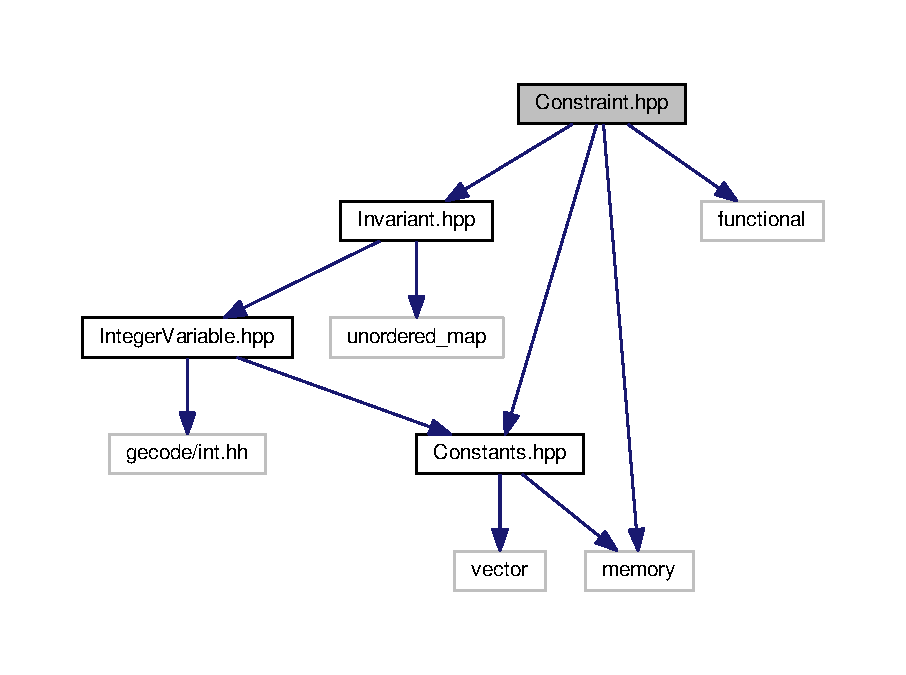
\includegraphics[width=350pt]{_constraint_8hpp__incl}
\end{center}
\end{figure}
This graph shows which files directly or indirectly include this file\-:
\nopagebreak
\begin{figure}[H]
\begin{center}
\leavevmode
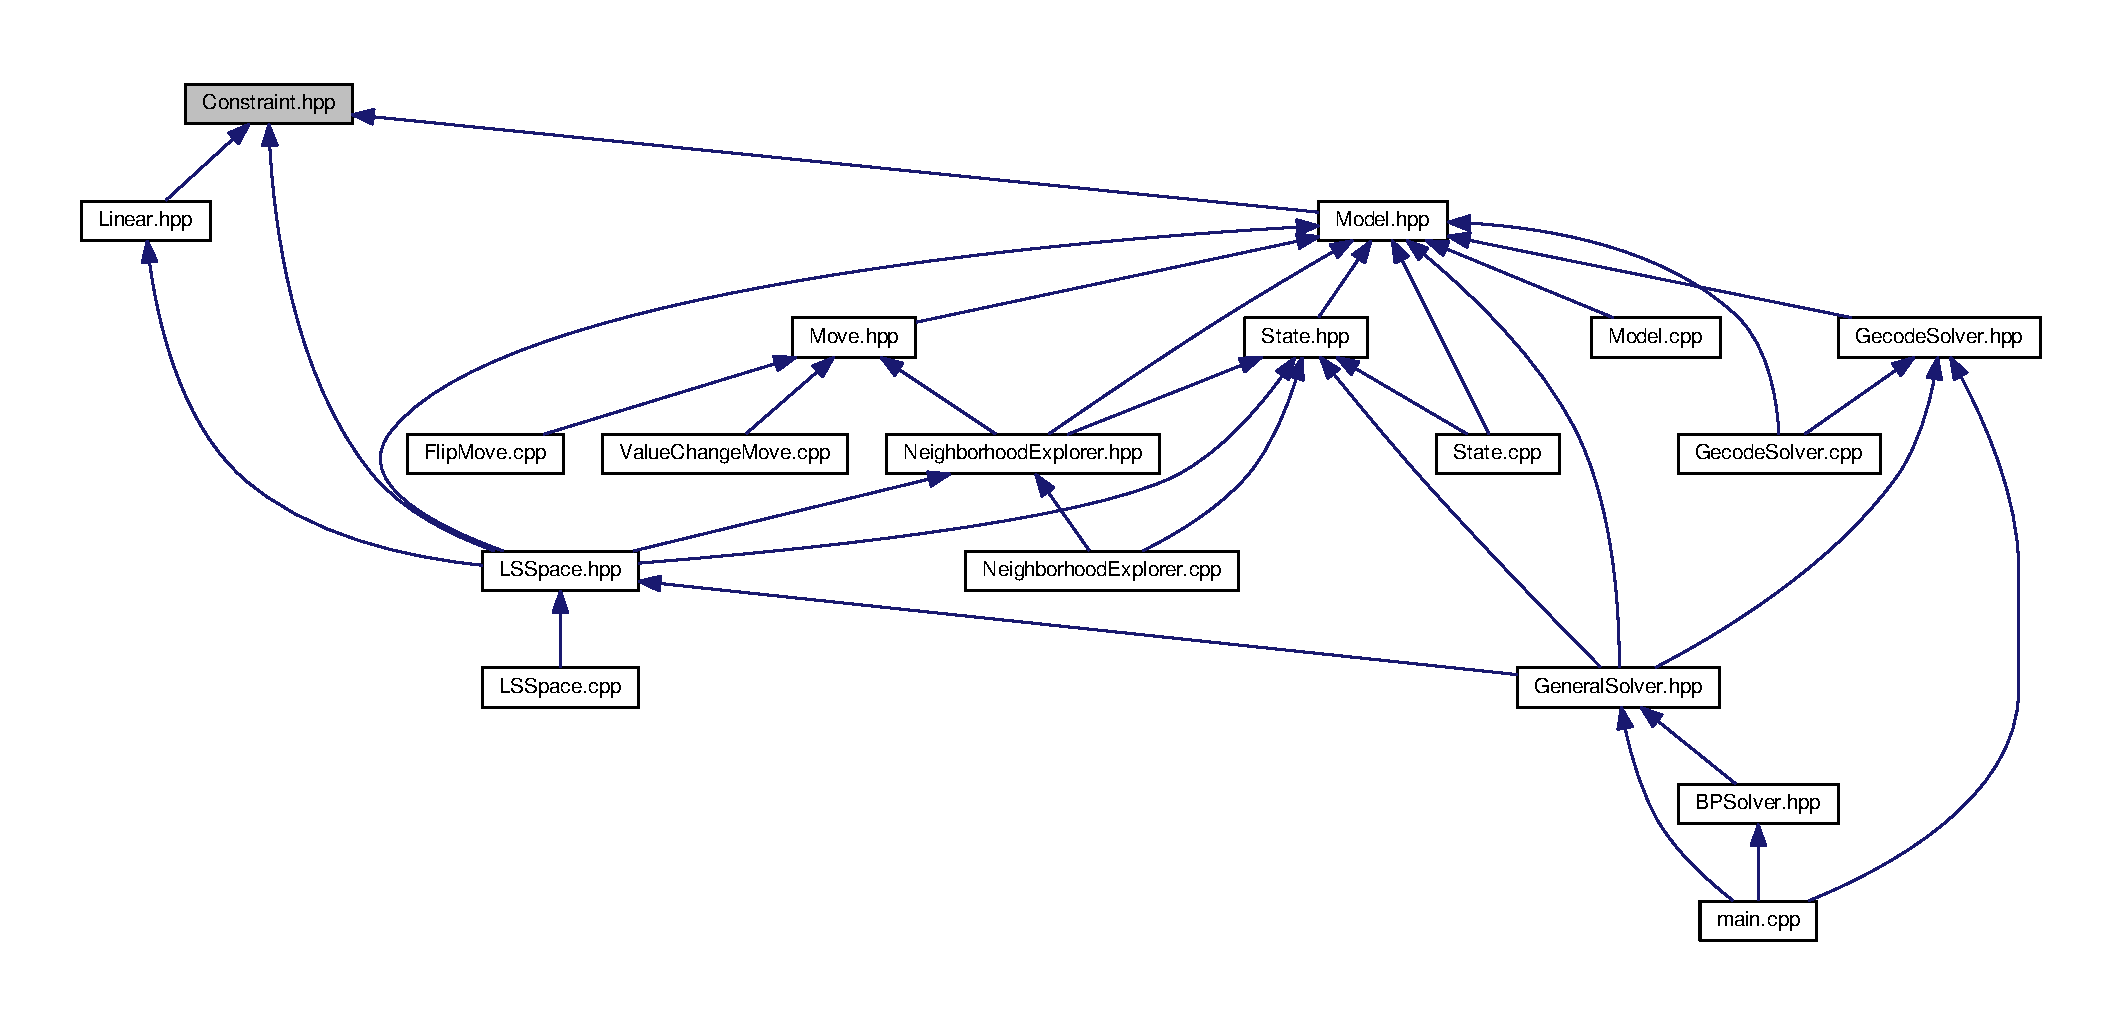
\includegraphics[width=350pt]{_constraint_8hpp__dep__incl}
\end{center}
\end{figure}
\subsection*{Classes}
\begin{DoxyCompactItemize}
\item 
class \hyperlink{class_constraint}{Constraint}
\item 
struct \hyperlink{struct_constraint_1_1_sort_greater}{Constraint\-::\-Sort\-Greater}
\item 
class \hyperlink{class_constraint_sorter}{Constraint\-Sorter}
\end{DoxyCompactItemize}

\hypertarget{_flip_move_8cpp}{\section{Flip\-Move.\-cpp File Reference}
\label{_flip_move_8cpp}\index{Flip\-Move.\-cpp@{Flip\-Move.\-cpp}}
}
{\ttfamily \#include \char`\"{}Flip\-Move.\-hpp\char`\"{}}\\*
{\ttfamily \#include \char`\"{}Move.\-hpp\char`\"{}}\\*
Include dependency graph for Flip\-Move.\-cpp\-:\nopagebreak
\begin{figure}[H]
\begin{center}
\leavevmode
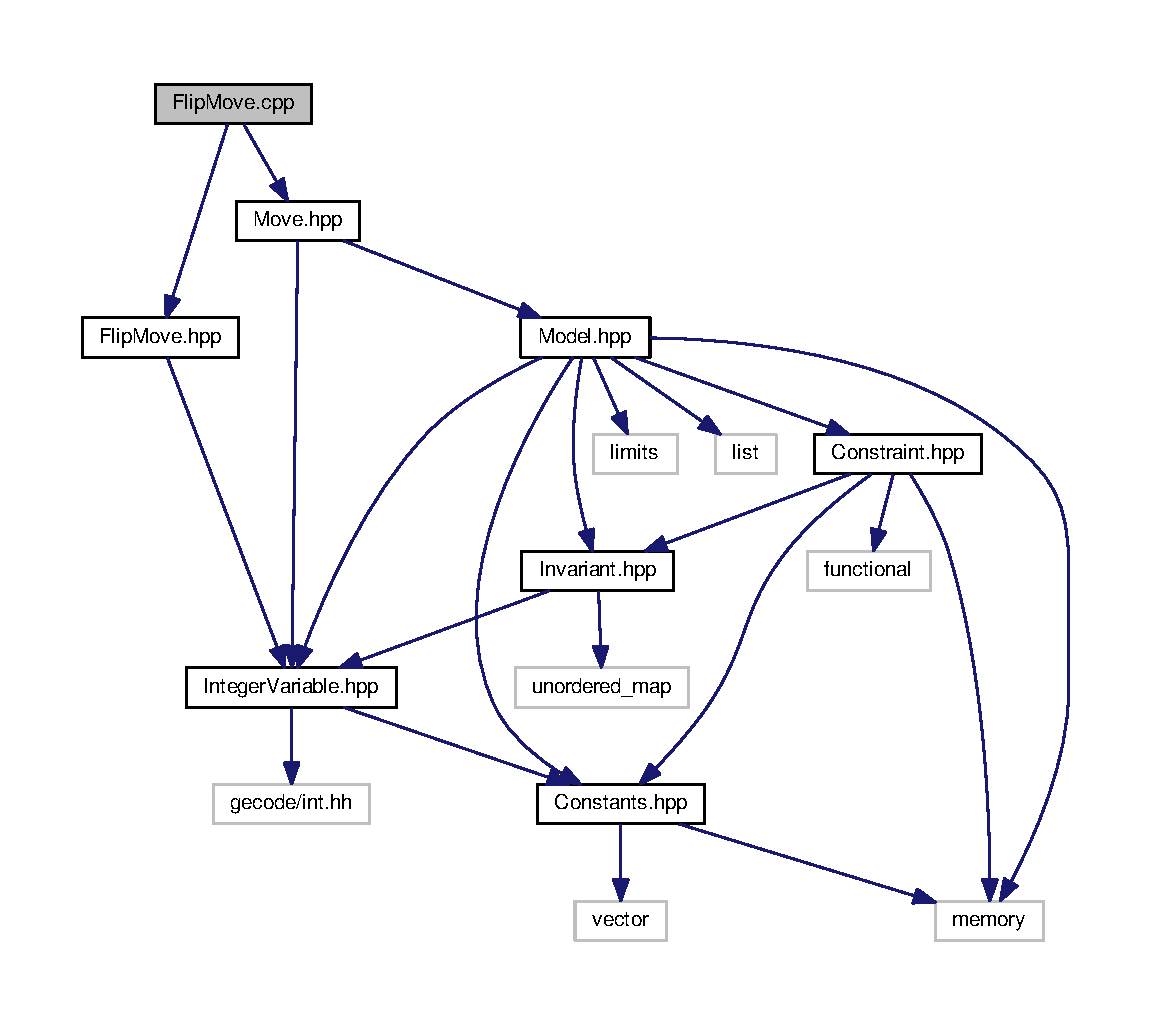
\includegraphics[width=350pt]{_flip_move_8cpp__incl}
\end{center}
\end{figure}

\hypertarget{_flip_move_8hpp}{\section{Flip\-Move.\-hpp File Reference}
\label{_flip_move_8hpp}\index{Flip\-Move.\-hpp@{Flip\-Move.\-hpp}}
}
{\ttfamily \#include \char`\"{}Integer\-Variable.\-hpp\char`\"{}}\\*
Include dependency graph for Flip\-Move.\-hpp\-:\nopagebreak
\begin{figure}[H]
\begin{center}
\leavevmode
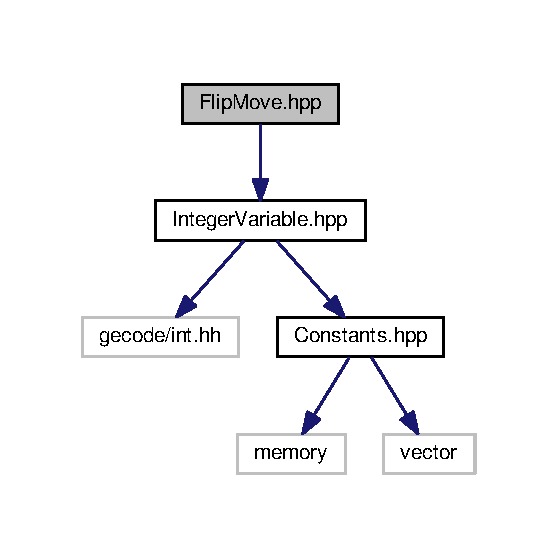
\includegraphics[width=267pt]{_flip_move_8hpp__incl}
\end{center}
\end{figure}
This graph shows which files directly or indirectly include this file\-:\nopagebreak
\begin{figure}[H]
\begin{center}
\leavevmode
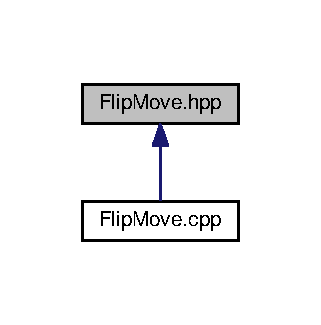
\includegraphics[width=154pt]{_flip_move_8hpp__dep__incl}
\end{center}
\end{figure}
\subsection*{Classes}
\begin{DoxyCompactItemize}
\item 
class \hyperlink{class_flip_move}{Flip\-Move}
\end{DoxyCompactItemize}

\hypertarget{_gecode_solver_8cpp}{\section{Gecode\-Solver.\-cpp File Reference}
\label{_gecode_solver_8cpp}\index{Gecode\-Solver.\-cpp@{Gecode\-Solver.\-cpp}}
}
{\ttfamily \#include $<$gecode/int.\-hh$>$}\\*
{\ttfamily \#include \char`\"{}Gecode\-Solver.\-hpp\char`\"{}}\\*
{\ttfamily \#include \char`\"{}Model.\-hpp\char`\"{}}\\*
Include dependency graph for Gecode\-Solver.\-cpp\-:\nopagebreak
\begin{figure}[H]
\begin{center}
\leavevmode
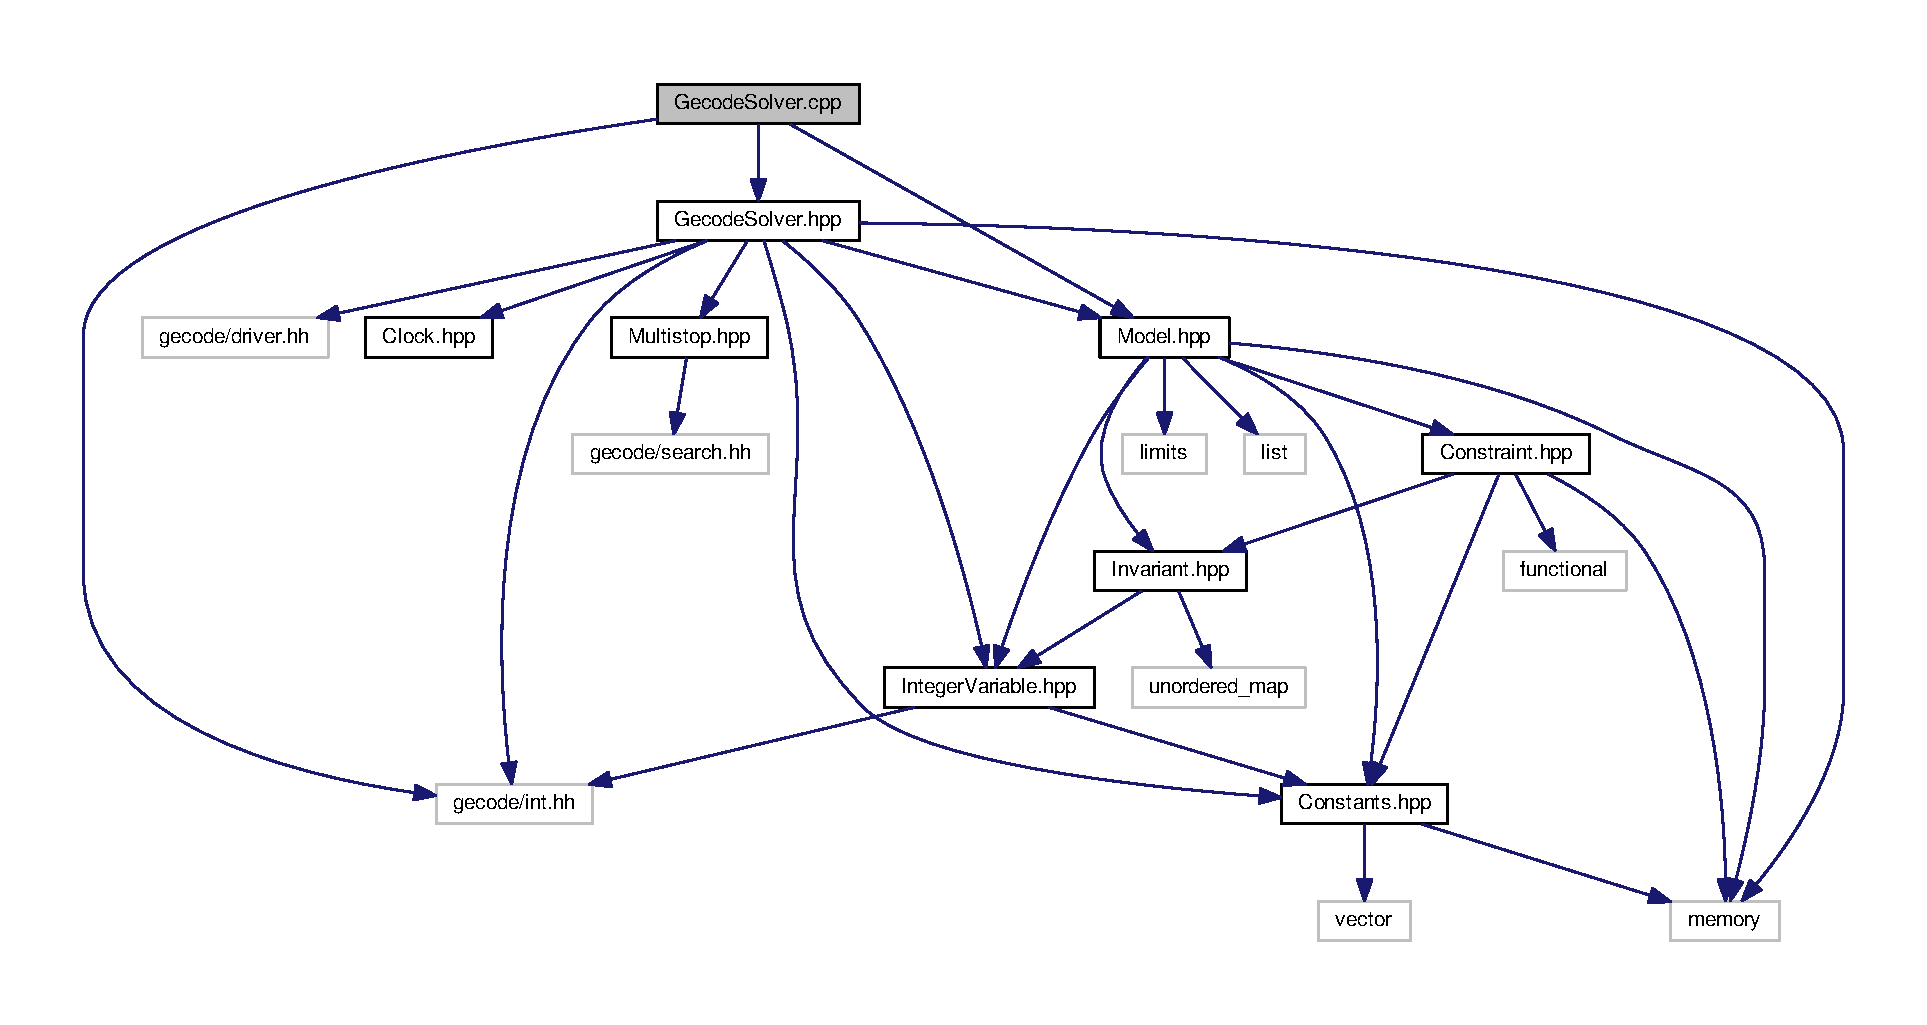
\includegraphics[width=350pt]{_gecode_solver_8cpp__incl}
\end{center}
\end{figure}

\hypertarget{_gecode_solver_8hpp}{\section{Gecode\-Solver.\-hpp File Reference}
\label{_gecode_solver_8hpp}\index{Gecode\-Solver.\-hpp@{Gecode\-Solver.\-hpp}}
}
{\ttfamily \#include $<$memory$>$}\\*
{\ttfamily \#include $<$gecode/driver.\-hh$>$}\\*
{\ttfamily \#include $<$gecode/int.\-hh$>$}\\*
{\ttfamily \#include \char`\"{}Integer\-Variable.\-hpp\char`\"{}}\\*
{\ttfamily \#include \char`\"{}Clock.\-hpp\char`\"{}}\\*
{\ttfamily \#include \char`\"{}Constants.\-hpp\char`\"{}}\\*
{\ttfamily \#include \char`\"{}Model.\-hpp\char`\"{}}\\*
{\ttfamily \#include \char`\"{}Multistop.\-hpp\char`\"{}}\\*
Include dependency graph for Gecode\-Solver.\-hpp\-:\nopagebreak
\begin{figure}[H]
\begin{center}
\leavevmode
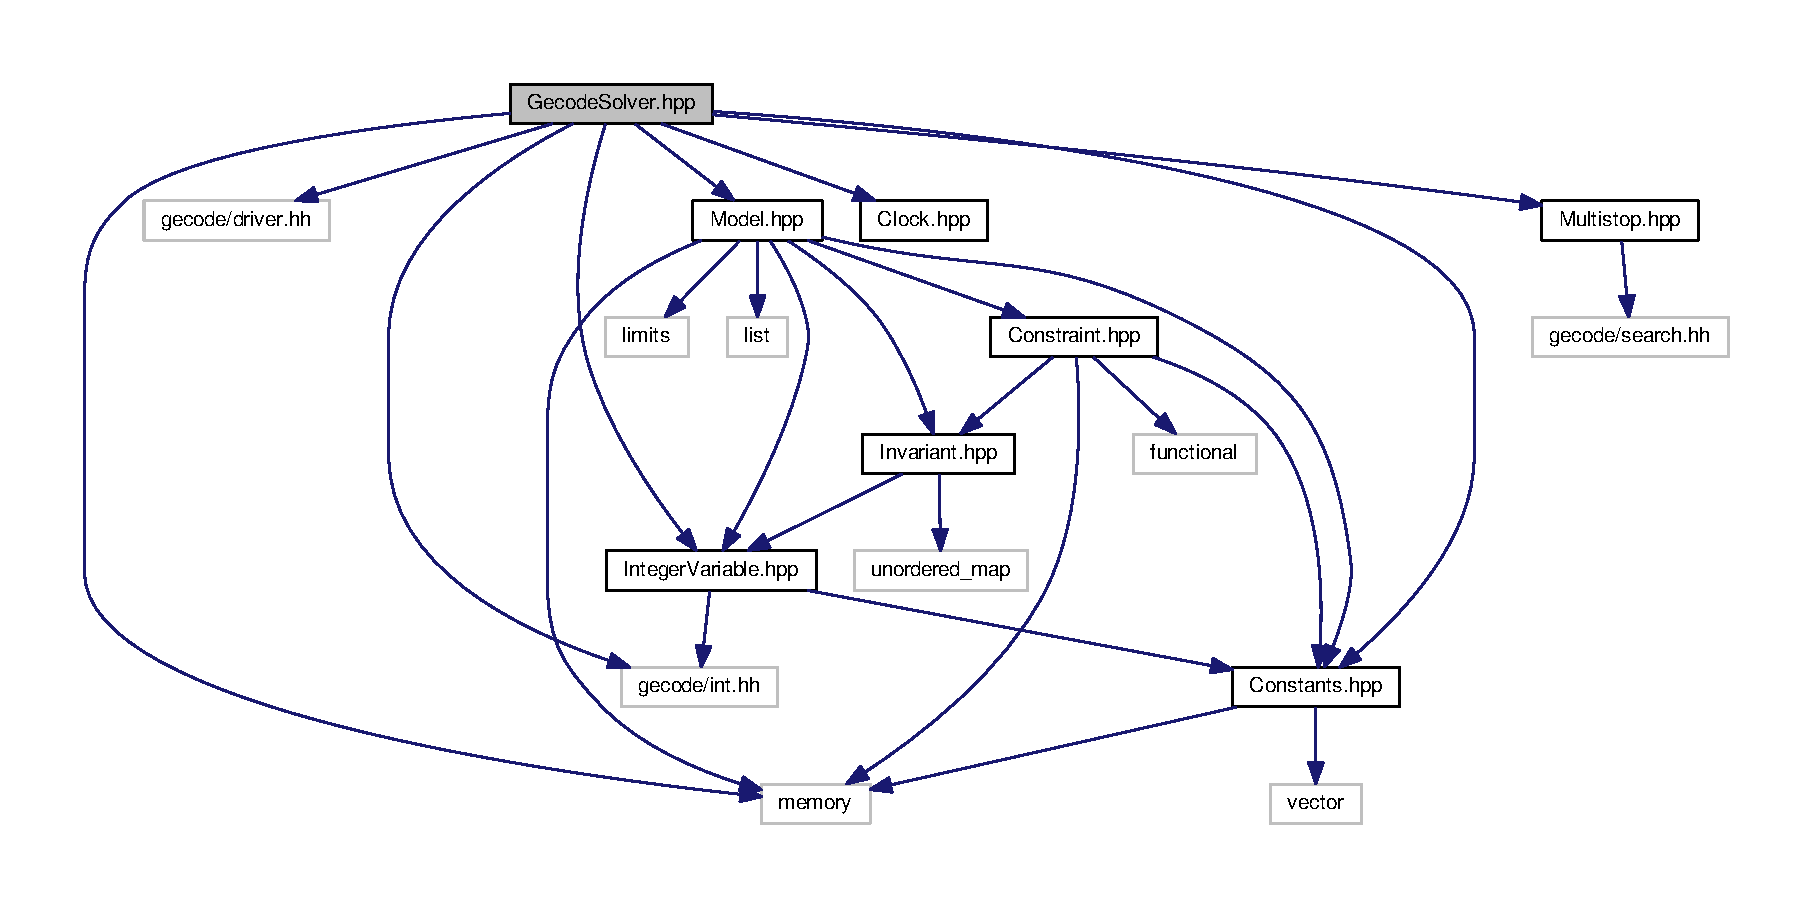
\includegraphics[width=350pt]{_gecode_solver_8hpp__incl}
\end{center}
\end{figure}
This graph shows which files directly or indirectly include this file\-:
\nopagebreak
\begin{figure}[H]
\begin{center}
\leavevmode
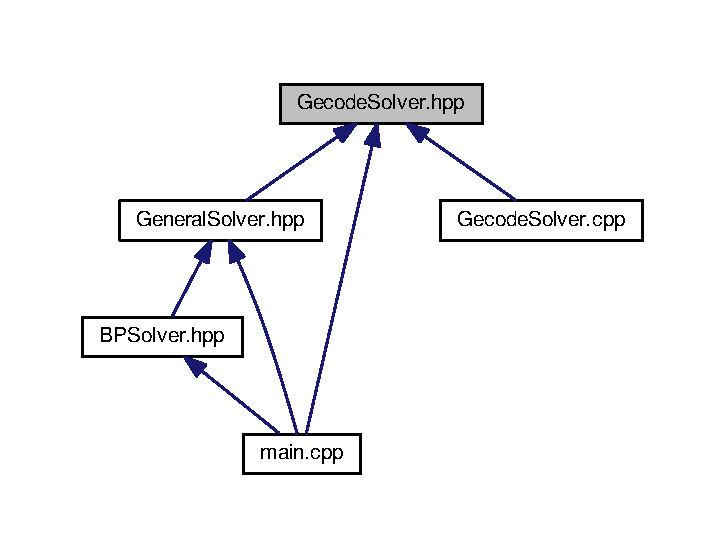
\includegraphics[width=348pt]{_gecode_solver_8hpp__dep__incl}
\end{center}
\end{figure}
\subsection*{Classes}
\begin{DoxyCompactItemize}
\item 
class \hyperlink{class_gecode_solver}{Gecode\-Solver}
\end{DoxyCompactItemize}

\hypertarget{_general_solver_8cpp}{\section{General\-Solver.\-cpp File Reference}
\label{_general_solver_8cpp}\index{General\-Solver.\-cpp@{General\-Solver.\-cpp}}
}

\hypertarget{_general_solver_8hpp}{\section{General\-Solver.\-hpp File Reference}
\label{_general_solver_8hpp}\index{General\-Solver.\-hpp@{General\-Solver.\-hpp}}
}
{\ttfamily \#include $<$cmath$>$}\\*
{\ttfamily \#include $<$algorithm$>$}\\*
{\ttfamily \#include \char`\"{}L\-S\-Space.\-hpp\char`\"{}}\\*
{\ttfamily \#include $<$assert.\-h$>$}\\*
{\ttfamily \#include \char`\"{}Model.\-hpp\char`\"{}}\\*
{\ttfamily \#include $<$gecode/driver.\-hh$>$}\\*
{\ttfamily \#include $<$gecode/int.\-hh$>$}\\*
{\ttfamily \#include \char`\"{}Constants.\-hpp\char`\"{}}\\*
{\ttfamily \#include \char`\"{}Gecode\-Solver.\-hpp\char`\"{}}\\*
{\ttfamily \#include $<$limits$>$}\\*
{\ttfamily \#include \char`\"{}Integer\-Variable.\-hpp\char`\"{}}\\*
{\ttfamily \#include \char`\"{}Multistop.\-hpp\char`\"{}}\\*
{\ttfamily \#include \char`\"{}Sum.\-hpp\char`\"{}}\\*
{\ttfamily \#include $<$memory$>$}\\*
{\ttfamily \#include \char`\"{}State.\-hpp\char`\"{}}\\*
{\ttfamily \#include $<$functional$>$}\\*
{\ttfamily \#include \char`\"{}Clock.\-hpp\char`\"{}}\\*
Include dependency graph for General\-Solver.\-hpp\-:\nopagebreak
\begin{figure}[H]
\begin{center}
\leavevmode
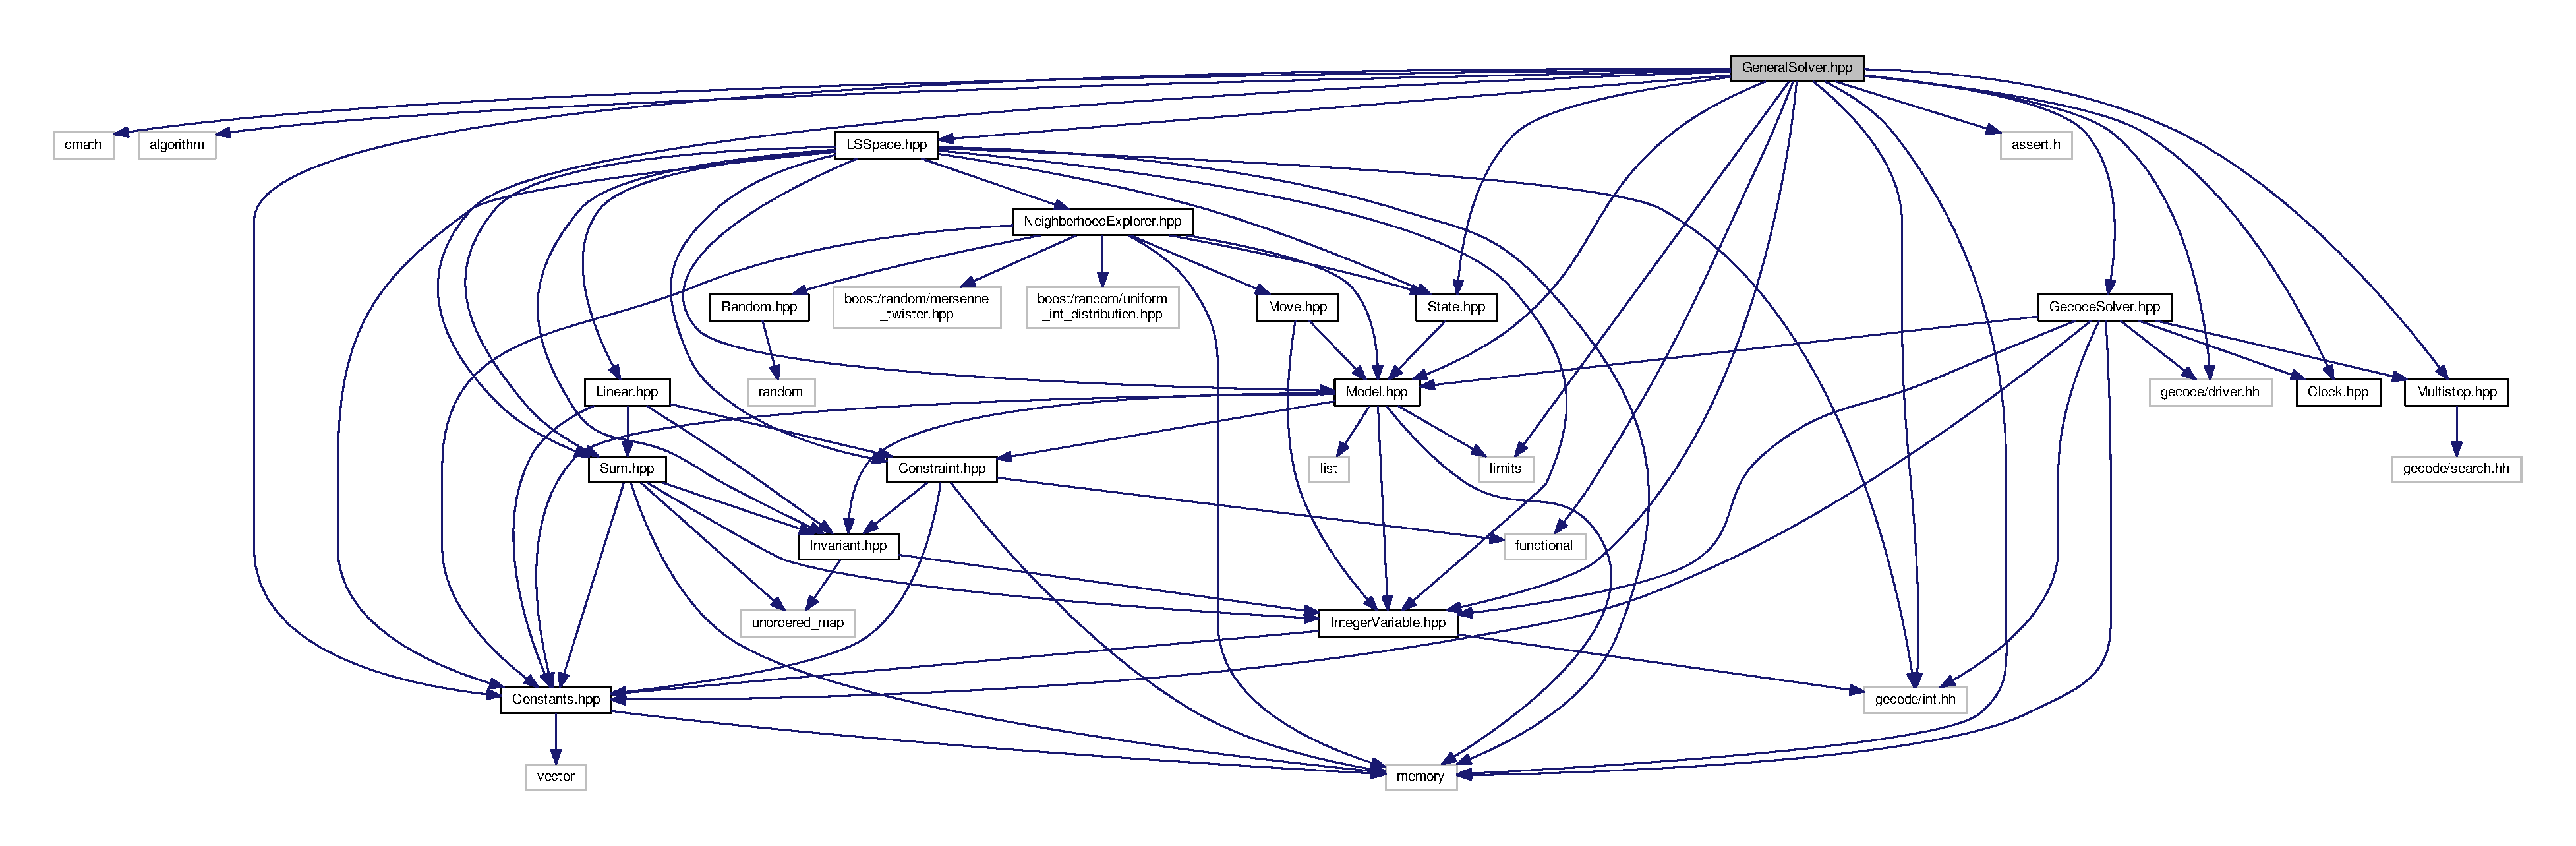
\includegraphics[width=350pt]{_general_solver_8hpp__incl}
\end{center}
\end{figure}
This graph shows which files directly or indirectly include this file\-:
\nopagebreak
\begin{figure}[H]
\begin{center}
\leavevmode
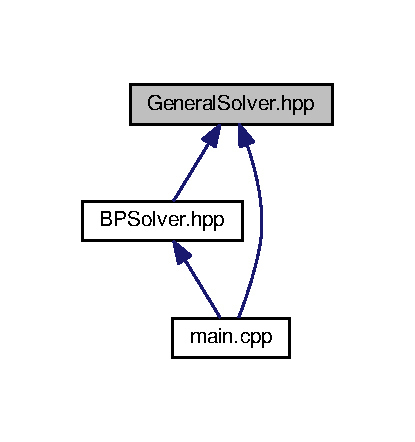
\includegraphics[width=199pt]{_general_solver_8hpp__dep__incl}
\end{center}
\end{figure}
\subsection*{Classes}
\begin{DoxyCompactItemize}
\item 
class \hyperlink{class_general_solver}{General\-Solver}
\end{DoxyCompactItemize}

\hypertarget{get_r_s_s_8hpp}{\section{get\-R\-S\-S.\-hpp File Reference}
\label{get_r_s_s_8hpp}\index{get\-R\-S\-S.\-hpp@{get\-R\-S\-S.\-hpp}}
}
This graph shows which files directly or indirectly include this file\-:\nopagebreak
\begin{figure}[H]
\begin{center}
\leavevmode
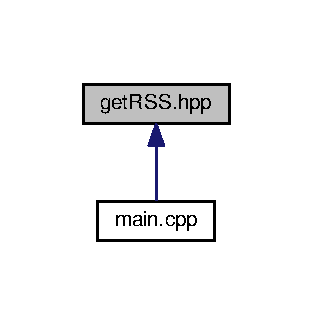
\includegraphics[width=150pt]{get_r_s_s_8hpp__dep__incl}
\end{center}
\end{figure}
\subsection*{Functions}
\begin{DoxyCompactItemize}
\item 
size\-\_\-t \hyperlink{get_r_s_s_8hpp_a4915f71ef0e010b76fb7fa6086233ec1}{get\-Peak\-R\-S\-S} ()
\item 
size\-\_\-t \hyperlink{get_r_s_s_8hpp_a04ca71f0a6ce75f1d8d1402edc70bcdc}{get\-Current\-R\-S\-S} ()
\end{DoxyCompactItemize}


\subsection{Function Documentation}
\hypertarget{get_r_s_s_8hpp_a04ca71f0a6ce75f1d8d1402edc70bcdc}{\index{get\-R\-S\-S.\-hpp@{get\-R\-S\-S.\-hpp}!get\-Current\-R\-S\-S@{get\-Current\-R\-S\-S}}
\index{get\-Current\-R\-S\-S@{get\-Current\-R\-S\-S}!getRSS.hpp@{get\-R\-S\-S.\-hpp}}
\subsubsection[{get\-Current\-R\-S\-S}]{\setlength{\rightskip}{0pt plus 5cm}size\-\_\-t get\-Current\-R\-S\-S (
\begin{DoxyParamCaption}
{}
\end{DoxyParamCaption}
)}}\label{get_r_s_s_8hpp_a04ca71f0a6ce75f1d8d1402edc70bcdc}
Returns the current resident set size (physical memory use) measured in bytes, or zero if the value cannot be determined on this O\-S. \hypertarget{get_r_s_s_8hpp_a4915f71ef0e010b76fb7fa6086233ec1}{\index{get\-R\-S\-S.\-hpp@{get\-R\-S\-S.\-hpp}!get\-Peak\-R\-S\-S@{get\-Peak\-R\-S\-S}}
\index{get\-Peak\-R\-S\-S@{get\-Peak\-R\-S\-S}!getRSS.hpp@{get\-R\-S\-S.\-hpp}}
\subsubsection[{get\-Peak\-R\-S\-S}]{\setlength{\rightskip}{0pt plus 5cm}size\-\_\-t get\-Peak\-R\-S\-S (
\begin{DoxyParamCaption}
{}
\end{DoxyParamCaption}
)}}\label{get_r_s_s_8hpp_a4915f71ef0e010b76fb7fa6086233ec1}
Returns the peak (maximum so far) resident set size (physical memory use) measured in bytes, or zero if the value cannot be determined on this O\-S. 
\hypertarget{_integer_variable_8cpp}{\section{Integer\-Variable.\-cpp File Reference}
\label{_integer_variable_8cpp}\index{Integer\-Variable.\-cpp@{Integer\-Variable.\-cpp}}
}

\hypertarget{_integer_variable_8hpp}{\section{Integer\-Variable.\-hpp File Reference}
\label{_integer_variable_8hpp}\index{Integer\-Variable.\-hpp@{Integer\-Variable.\-hpp}}
}
{\ttfamily \#include $<$gecode/int.\-hh$>$}\\*
{\ttfamily \#include \char`\"{}Constants.\-hpp\char`\"{}}\\*
Include dependency graph for Integer\-Variable.\-hpp\-:\nopagebreak
\begin{figure}[H]
\begin{center}
\leavevmode
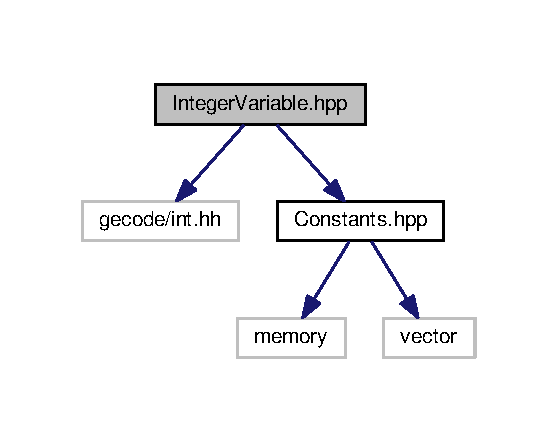
\includegraphics[width=267pt]{_integer_variable_8hpp__incl}
\end{center}
\end{figure}
This graph shows which files directly or indirectly include this file\-:
\nopagebreak
\begin{figure}[H]
\begin{center}
\leavevmode
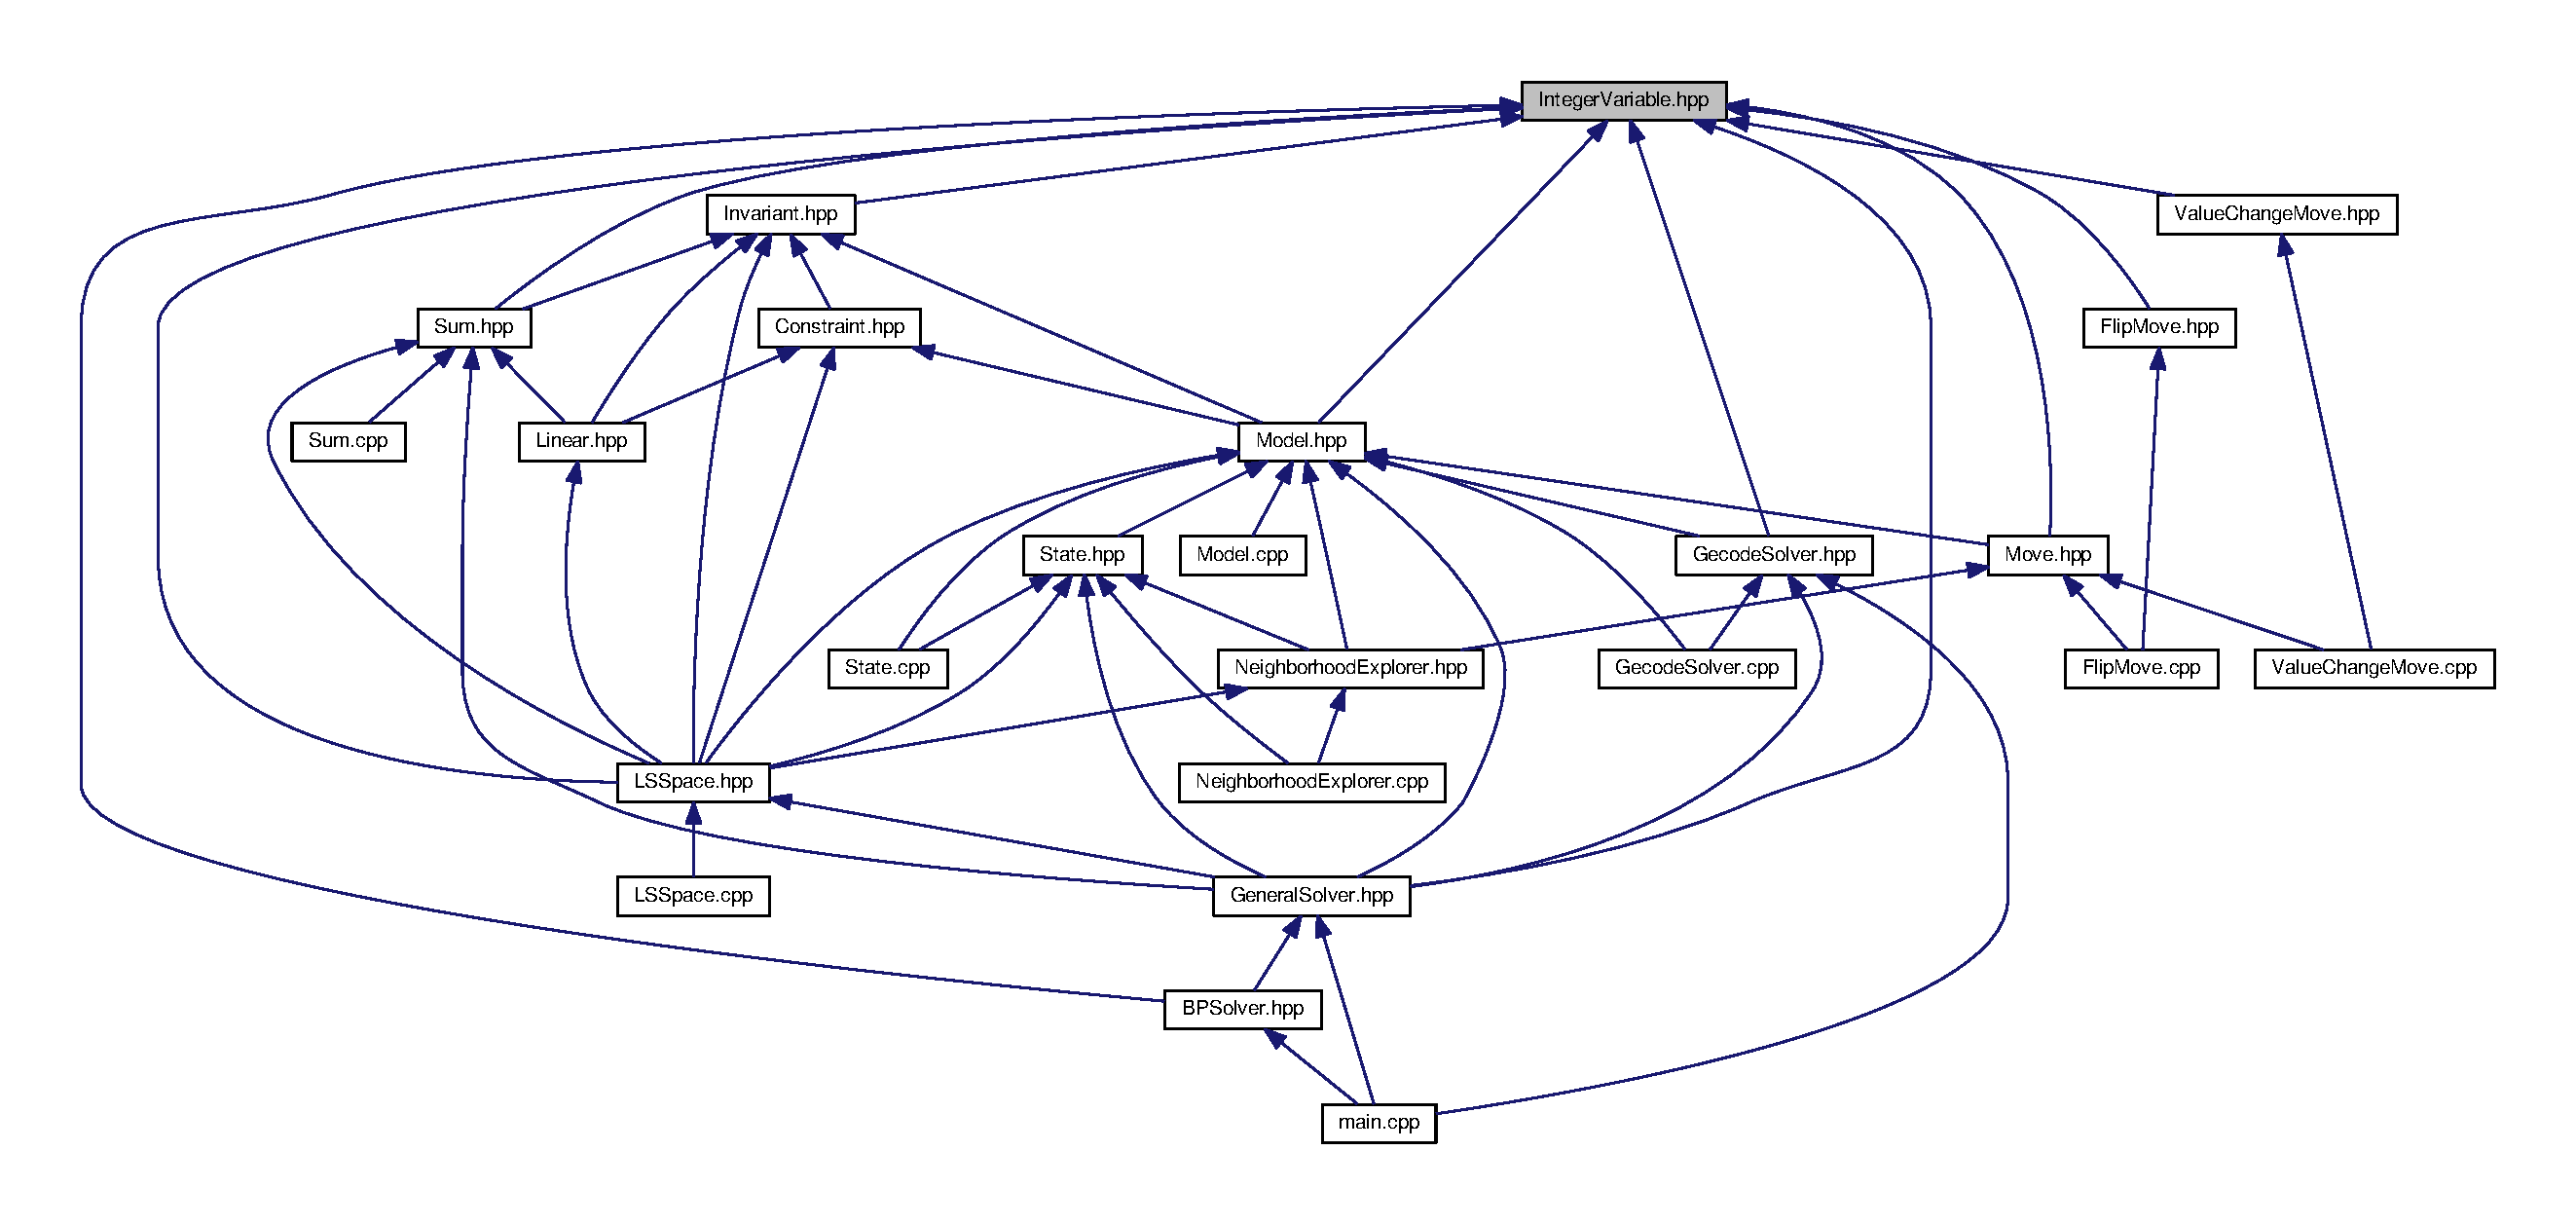
\includegraphics[width=350pt]{_integer_variable_8hpp__dep__incl}
\end{center}
\end{figure}
\subsection*{Classes}
\begin{DoxyCompactItemize}
\item 
class \hyperlink{class_integer_variable}{Integer\-Variable}
\end{DoxyCompactItemize}

\hypertarget{_invariant_8hpp}{\section{Invariant.\-hpp File Reference}
\label{_invariant_8hpp}\index{Invariant.\-hpp@{Invariant.\-hpp}}
}
{\ttfamily \#include \char`\"{}Integer\-Variable.\-hpp\char`\"{}}\\*
{\ttfamily \#include $<$unordered\-\_\-map$>$}\\*
Include dependency graph for Invariant.\-hpp\-:\nopagebreak
\begin{figure}[H]
\begin{center}
\leavevmode
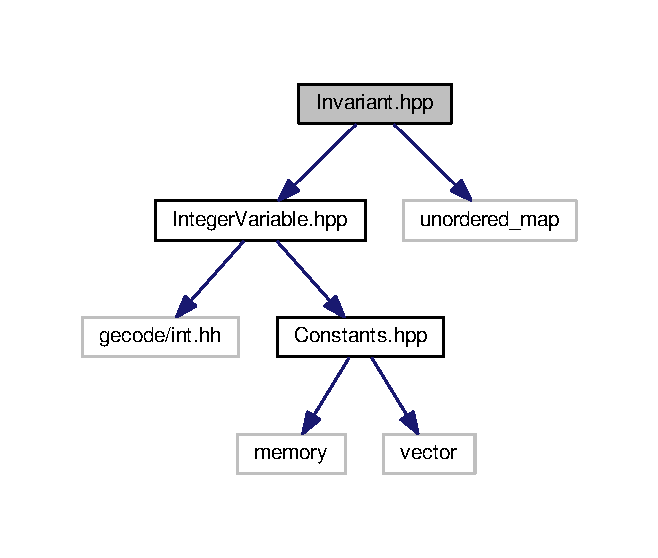
\includegraphics[width=316pt]{_invariant_8hpp__incl}
\end{center}
\end{figure}
This graph shows which files directly or indirectly include this file\-:
\nopagebreak
\begin{figure}[H]
\begin{center}
\leavevmode
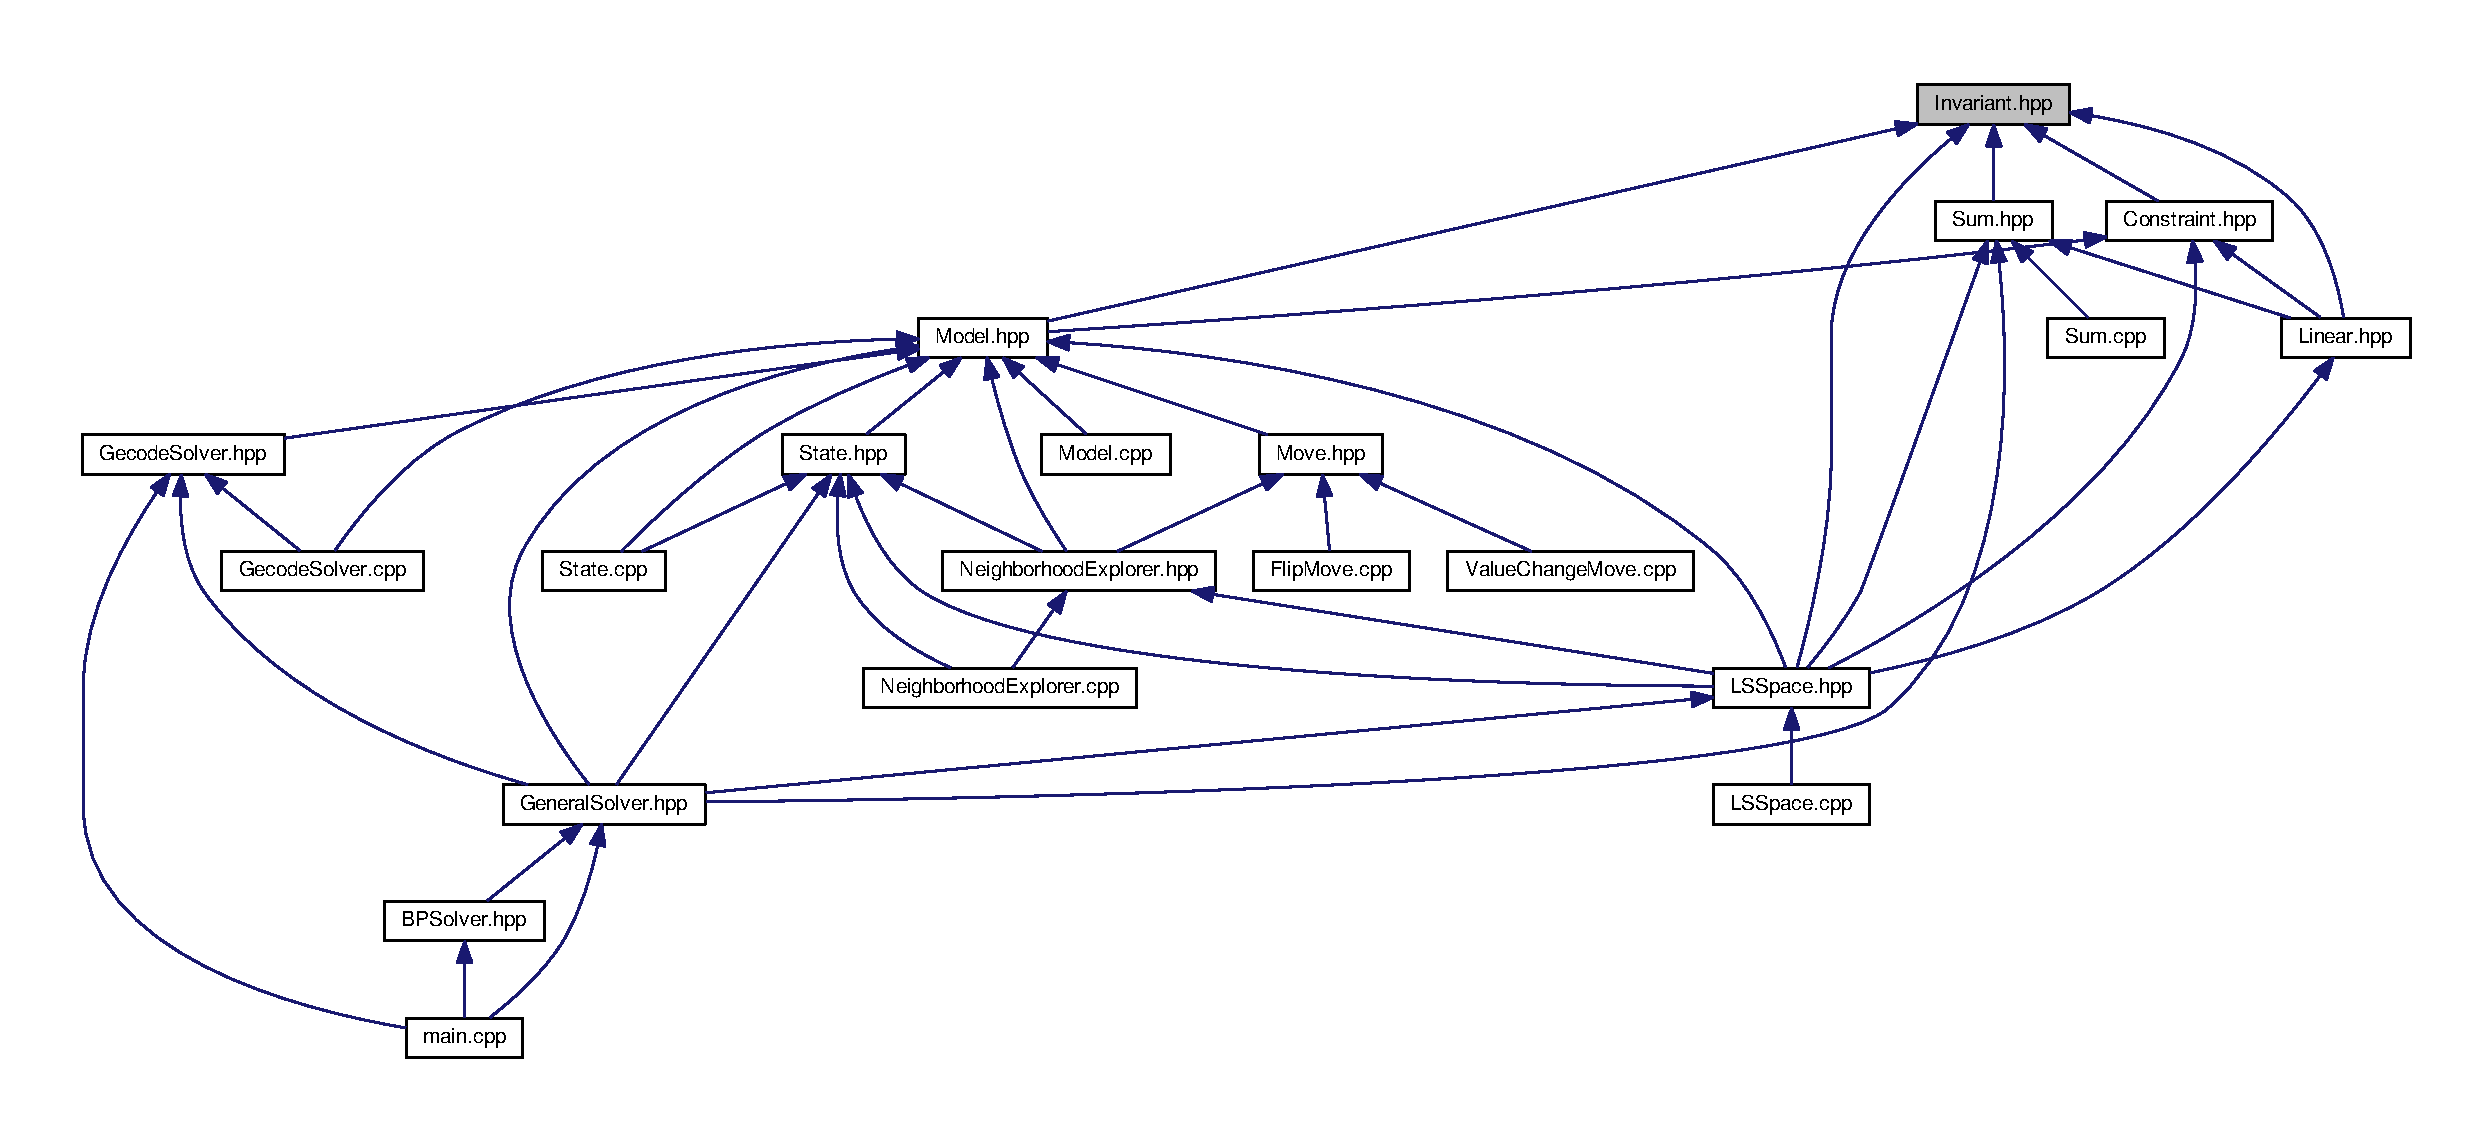
\includegraphics[width=350pt]{_invariant_8hpp__dep__incl}
\end{center}
\end{figure}
\subsection*{Classes}
\begin{DoxyCompactItemize}
\item 
class \hyperlink{class_invariant}{Invariant}
\end{DoxyCompactItemize}

\hypertarget{_linear_8hpp}{\section{Linear.\-hpp File Reference}
\label{_linear_8hpp}\index{Linear.\-hpp@{Linear.\-hpp}}
}
{\ttfamily \#include \char`\"{}Sum.\-hpp\char`\"{}}\\*
{\ttfamily \#include \char`\"{}Invariant.\-hpp\char`\"{}}\\*
{\ttfamily \#include \char`\"{}Constraint.\-hpp\char`\"{}}\\*
{\ttfamily \#include \char`\"{}Constants.\-hpp\char`\"{}}\\*
Include dependency graph for Linear.\-hpp\-:\nopagebreak
\begin{figure}[H]
\begin{center}
\leavevmode
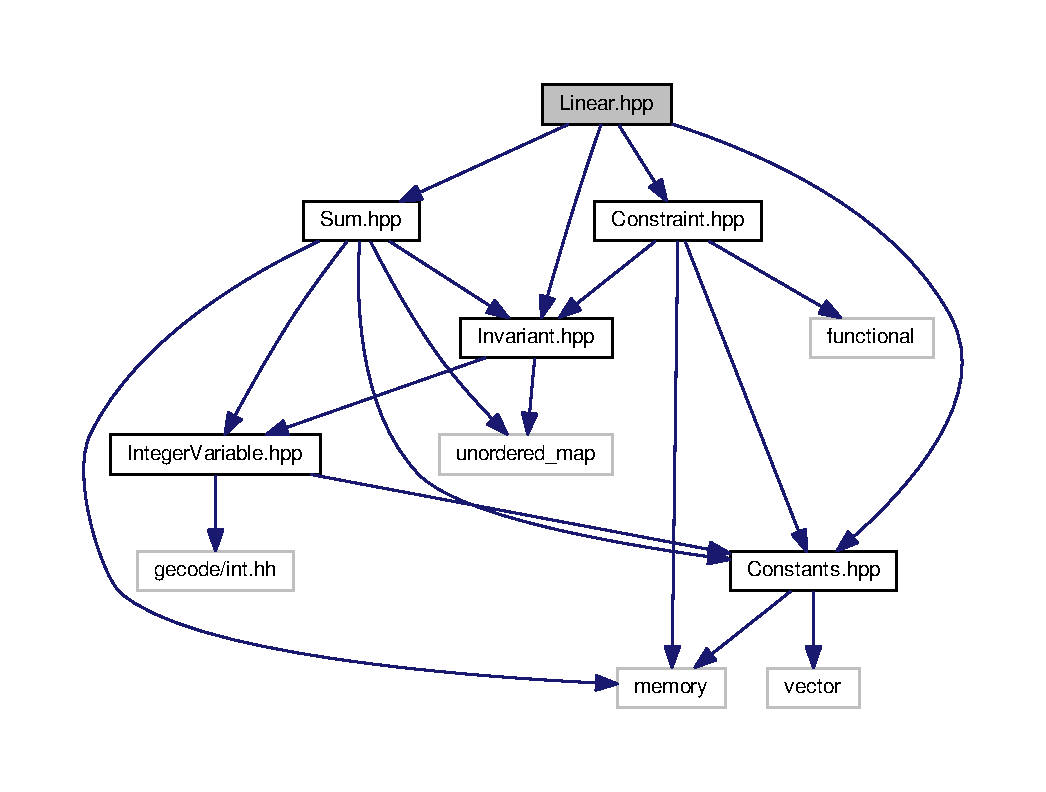
\includegraphics[width=350pt]{_linear_8hpp__incl}
\end{center}
\end{figure}
This graph shows which files directly or indirectly include this file\-:
\nopagebreak
\begin{figure}[H]
\begin{center}
\leavevmode
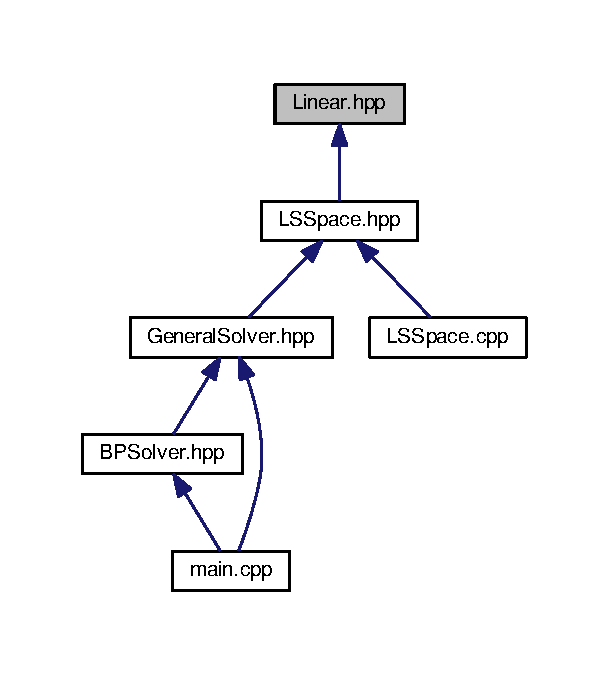
\includegraphics[width=292pt]{_linear_8hpp__dep__incl}
\end{center}
\end{figure}
\subsection*{Classes}
\begin{DoxyCompactItemize}
\item 
class \hyperlink{class_linear}{Linear}
\end{DoxyCompactItemize}

\hypertarget{_l_s_space_8cpp}{\section{L\-S\-Space.\-cpp File Reference}
\label{_l_s_space_8cpp}\index{L\-S\-Space.\-cpp@{L\-S\-Space.\-cpp}}
}
{\ttfamily \#include \char`\"{}L\-S\-Space.\-hpp\char`\"{}}\\*
Include dependency graph for L\-S\-Space.\-cpp\-:\nopagebreak
\begin{figure}[H]
\begin{center}
\leavevmode
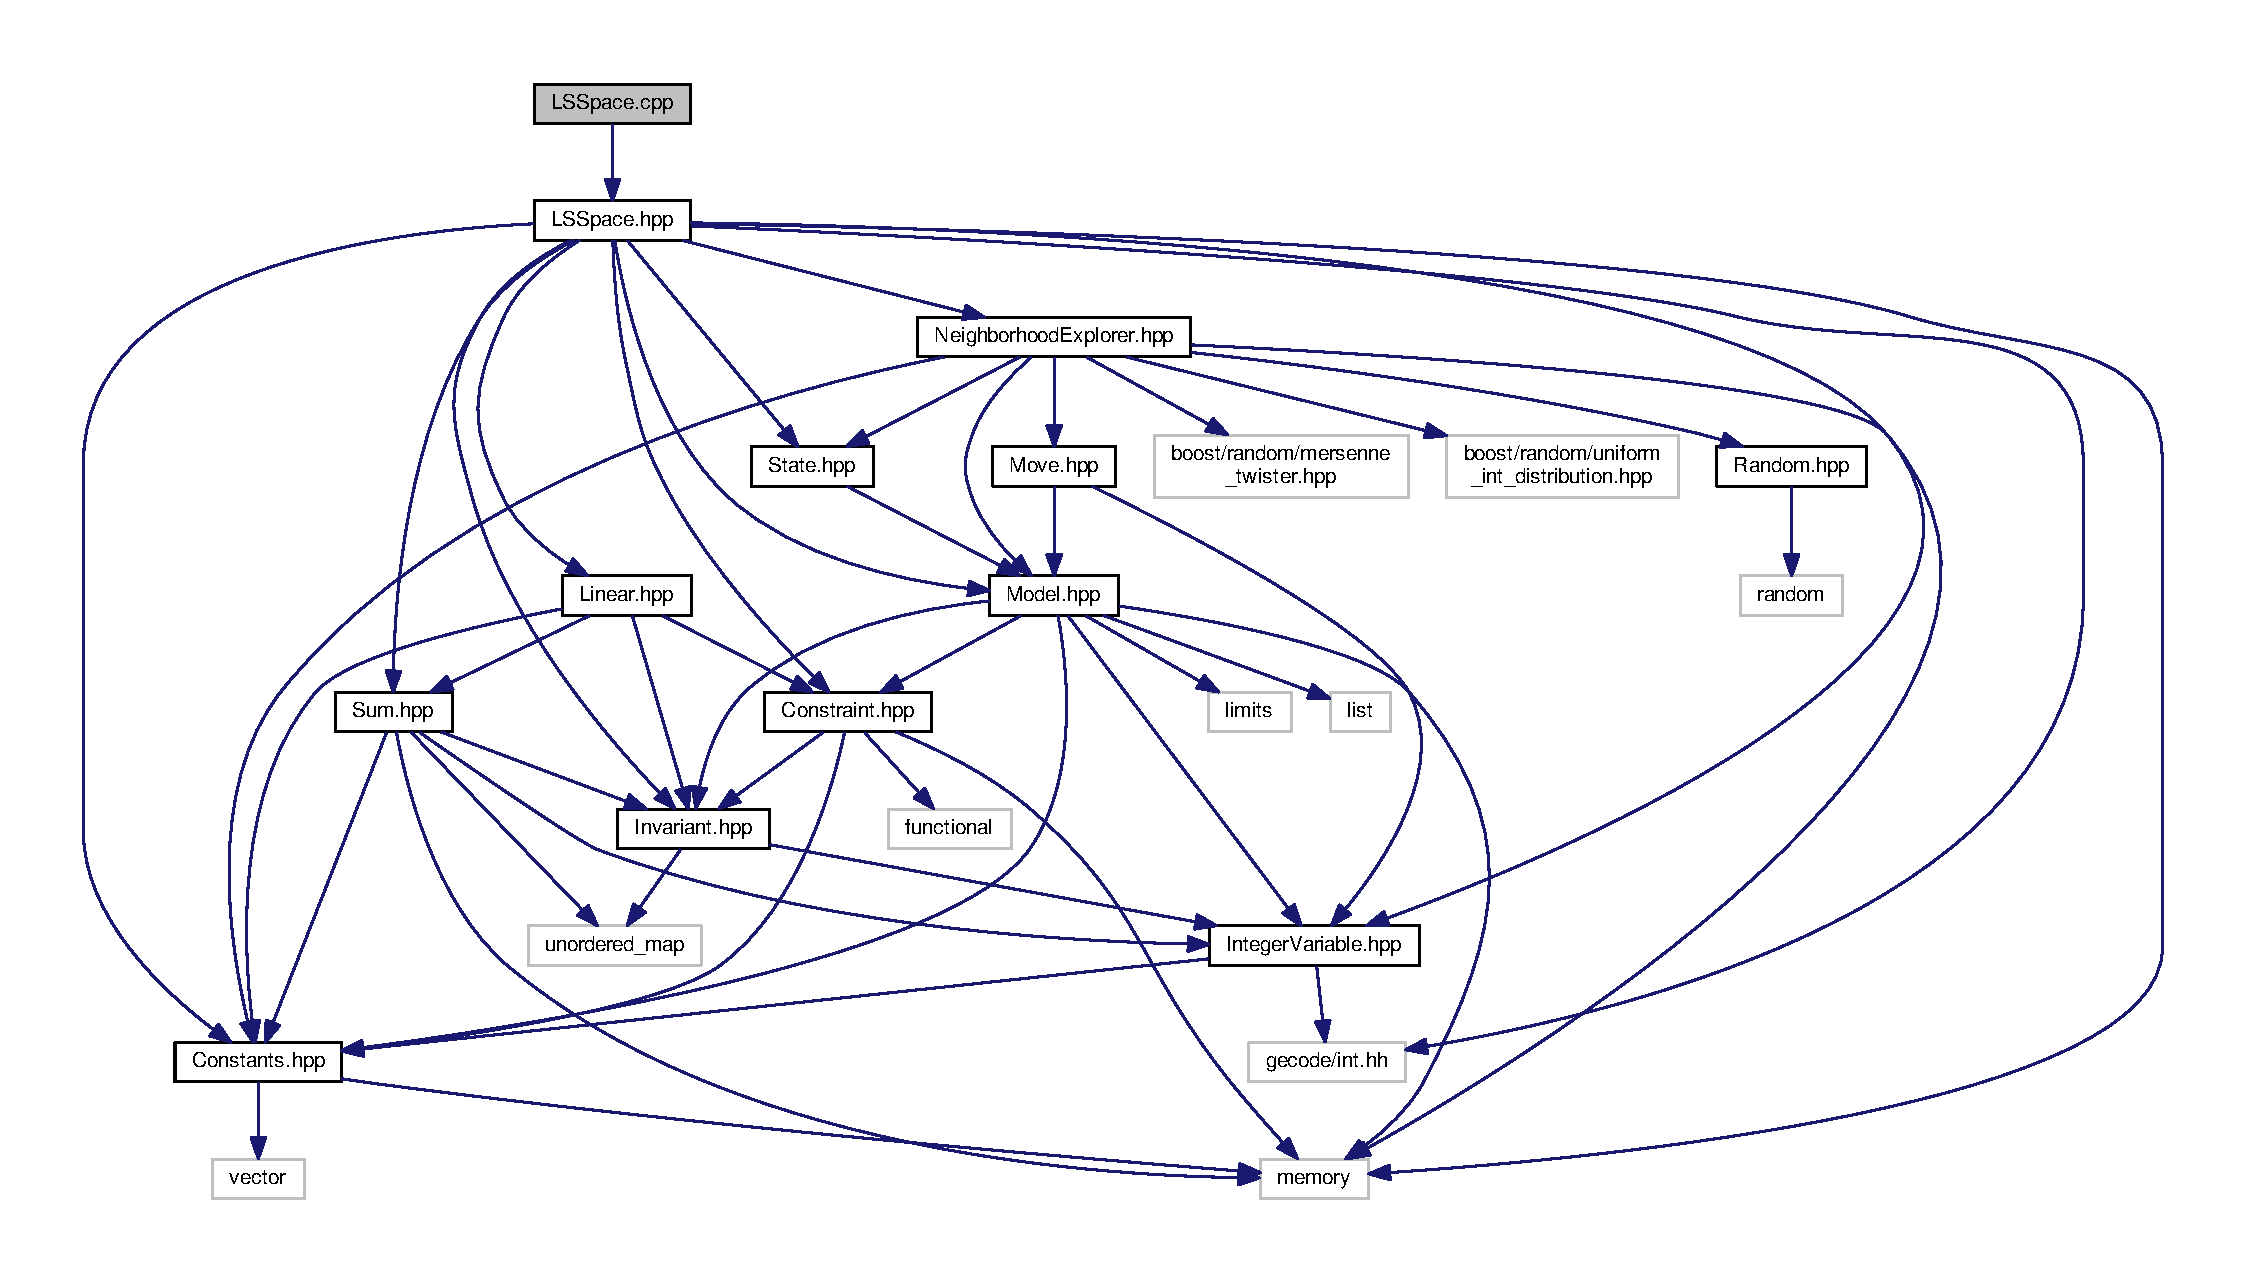
\includegraphics[width=350pt]{_l_s_space_8cpp__incl}
\end{center}
\end{figure}

\hypertarget{_l_s_space_8hpp}{\section{L\-S\-Space.\-hpp File Reference}
\label{_l_s_space_8hpp}\index{L\-S\-Space.\-hpp@{L\-S\-Space.\-hpp}}
}
{\ttfamily \#include $<$gecode/int.\-hh$>$}\\*
{\ttfamily \#include \char`\"{}Integer\-Variable.\-hpp\char`\"{}}\\*
{\ttfamily \#include \char`\"{}Invariant.\-hpp\char`\"{}}\\*
{\ttfamily \#include \char`\"{}Constraint.\-hpp\char`\"{}}\\*
{\ttfamily \#include \char`\"{}Sum.\-hpp\char`\"{}}\\*
{\ttfamily \#include \char`\"{}Linear.\-hpp\char`\"{}}\\*
{\ttfamily \#include \char`\"{}Model.\-hpp\char`\"{}}\\*
{\ttfamily \#include \char`\"{}Neighborhood\-Explorer.\-hpp\char`\"{}}\\*
{\ttfamily \#include \char`\"{}Constants.\-hpp\char`\"{}}\\*
{\ttfamily \#include $<$memory$>$}\\*
{\ttfamily \#include \char`\"{}State.\-hpp\char`\"{}}\\*
Include dependency graph for L\-S\-Space.\-hpp\-:\nopagebreak
\begin{figure}[H]
\begin{center}
\leavevmode
\includegraphics[width=350pt]{_l_s_space_8hpp__incl}
\end{center}
\end{figure}
This graph shows which files directly or indirectly include this file\-:
\nopagebreak
\begin{figure}[H]
\begin{center}
\leavevmode
\includegraphics[width=292pt]{_l_s_space_8hpp__dep__incl}
\end{center}
\end{figure}
\subsection*{Classes}
\begin{DoxyCompactItemize}
\item 
class \hyperlink{class_l_s_space}{L\-S\-Space}
\end{DoxyCompactItemize}

\hypertarget{main_8cpp}{\section{main.\-cpp File Reference}
\label{main_8cpp}\index{main.\-cpp@{main.\-cpp}}
}
{\ttfamily \#include $<$gecode/driver.\-hh$>$}\\*
{\ttfamily \#include $<$gecode/int.\-hh$>$}\\*
{\ttfamily \#include \char`\"{}B\-P\-\_\-\-Data.\-hpp\char`\"{}}\\*
{\ttfamily \#include $<$cmath$>$}\\*
{\ttfamily \#include $<$algorithm$>$}\\*
{\ttfamily \#include $<$limits$>$}\\*
{\ttfamily \#include \char`\"{}B\-P\-Solver.\-hpp\char`\"{}}\\*
{\ttfamily \#include \char`\"{}Clock.\-hpp\char`\"{}}\\*
{\ttfamily \#include \char`\"{}get\-R\-S\-S.\-hpp\char`\"{}}\\*
{\ttfamily \#include \char`\"{}General\-Solver.\-hpp\char`\"{}}\\*
{\ttfamily \#include \char`\"{}Gecode\-Solver.\-hpp\char`\"{}}\\*
{\ttfamily \#include \char`\"{}Test.\-hpp\char`\"{}}\\*
{\ttfamily \#include \char`\"{}Multistop.\-hpp\char`\"{}}\\*
{\ttfamily \#include $<$boost/algorithm/string.\-hpp$>$}\\*
Include dependency graph for main.\-cpp\-:
\nopagebreak
\begin{figure}[H]
\begin{center}
\leavevmode
\includegraphics[width=350pt]{main_8cpp__incl}
\end{center}
\end{figure}
\subsection*{Functions}
\begin{DoxyCompactItemize}
\item 
int \hyperlink{main_8cpp_a0ddf1224851353fc92bfbff6f499fa97}{main} (int argc, char $\ast$argv\mbox{[}$\,$\mbox{]})
\end{DoxyCompactItemize}


\subsection{Function Documentation}
\hypertarget{main_8cpp_a0ddf1224851353fc92bfbff6f499fa97}{\index{main.\-cpp@{main.\-cpp}!main@{main}}
\index{main@{main}!main.cpp@{main.\-cpp}}
\subsubsection[{main}]{\setlength{\rightskip}{0pt plus 5cm}int main (
\begin{DoxyParamCaption}
\item[{int}]{argc, }
\item[{char $\ast$}]{argv\mbox{[}$\,$\mbox{]}}
\end{DoxyParamCaption}
)}}\label{main_8cpp_a0ddf1224851353fc92bfbff6f499fa97}

\hypertarget{_model_8cpp}{\section{Model.\-cpp File Reference}
\label{_model_8cpp}\index{Model.\-cpp@{Model.\-cpp}}
}
{\ttfamily \#include \char`\"{}Model.\-hpp\char`\"{}}\\*
{\ttfamily \#include \char`\"{}Random.\-hpp\char`\"{}}\\*
Include dependency graph for Model.\-cpp\-:\nopagebreak
\begin{figure}[H]
\begin{center}
\leavevmode
\includegraphics[width=350pt]{_model_8cpp__incl}
\end{center}
\end{figure}

\hypertarget{_model_8hpp}{\section{Model.\-hpp File Reference}
\label{_model_8hpp}\index{Model.\-hpp@{Model.\-hpp}}
}
{\ttfamily \#include \char`\"{}Integer\-Variable.\-hpp\char`\"{}}\\*
{\ttfamily \#include \char`\"{}Invariant.\-hpp\char`\"{}}\\*
{\ttfamily \#include \char`\"{}Constraint.\-hpp\char`\"{}}\\*
{\ttfamily \#include \char`\"{}Constants.\-hpp\char`\"{}}\\*
{\ttfamily \#include $<$limits$>$}\\*
{\ttfamily \#include $<$memory$>$}\\*
{\ttfamily \#include $<$list$>$}\\*
Include dependency graph for Model.\-hpp\-:\nopagebreak
\begin{figure}[H]
\begin{center}
\leavevmode
\includegraphics[width=350pt]{_model_8hpp__incl}
\end{center}
\end{figure}
This graph shows which files directly or indirectly include this file\-:
\nopagebreak
\begin{figure}[H]
\begin{center}
\leavevmode
\includegraphics[width=350pt]{_model_8hpp__dep__incl}
\end{center}
\end{figure}
\subsection*{Classes}
\begin{DoxyCompactItemize}
\item 
class \hyperlink{class_model}{Model}
\end{DoxyCompactItemize}

\hypertarget{_move_8hpp}{\section{Move.\-hpp File Reference}
\label{_move_8hpp}\index{Move.\-hpp@{Move.\-hpp}}
}
{\ttfamily \#include \char`\"{}Model.\-hpp\char`\"{}}\\*
{\ttfamily \#include \char`\"{}Integer\-Variable.\-hpp\char`\"{}}\\*
Include dependency graph for Move.\-hpp\-:\nopagebreak
\begin{figure}[H]
\begin{center}
\leavevmode
\includegraphics[width=350pt]{_move_8hpp__incl}
\end{center}
\end{figure}
This graph shows which files directly or indirectly include this file\-:
\nopagebreak
\begin{figure}[H]
\begin{center}
\leavevmode
\includegraphics[width=350pt]{_move_8hpp__dep__incl}
\end{center}
\end{figure}
\subsection*{Classes}
\begin{DoxyCompactItemize}
\item 
class \hyperlink{class_move}{Move}
\end{DoxyCompactItemize}

\hypertarget{_multistop_8cpp}{\section{Multistop.\-cpp File Reference}
\label{_multistop_8cpp}\index{Multistop.\-cpp@{Multistop.\-cpp}}
}
{\ttfamily \#include \char`\"{}Multistop.\-hpp\char`\"{}}\\*
Include dependency graph for Multistop.\-cpp\-:\nopagebreak
\begin{figure}[H]
\begin{center}
\leavevmode
\includegraphics[width=174pt]{_multistop_8cpp__incl}
\end{center}
\end{figure}

\hypertarget{_multistop_8hpp}{\section{Multistop.\-hpp File Reference}
\label{_multistop_8hpp}\index{Multistop.\-hpp@{Multistop.\-hpp}}
}
{\ttfamily \#include $<$gecode/search.\-hh$>$}\\*
Include dependency graph for Multistop.\-hpp\-:\nopagebreak
\begin{figure}[H]
\begin{center}
\leavevmode
\includegraphics[width=174pt]{_multistop_8hpp__incl}
\end{center}
\end{figure}
This graph shows which files directly or indirectly include this file\-:
\nopagebreak
\begin{figure}[H]
\begin{center}
\leavevmode
\includegraphics[width=350pt]{_multistop_8hpp__dep__incl}
\end{center}
\end{figure}
\subsection*{Classes}
\begin{DoxyCompactItemize}
\item 
class \hyperlink{class_multistop}{Multistop}
\end{DoxyCompactItemize}

\hypertarget{_neighborhood_explorer_8cpp}{\section{Neighborhood\-Explorer.\-cpp File Reference}
\label{_neighborhood_explorer_8cpp}\index{Neighborhood\-Explorer.\-cpp@{Neighborhood\-Explorer.\-cpp}}
}
{\ttfamily \#include \char`\"{}Neighborhood\-Explorer.\-hpp\char`\"{}}\\*
{\ttfamily \#include \char`\"{}State.\-hpp\char`\"{}}\\*
Include dependency graph for Neighborhood\-Explorer.\-cpp\-:\nopagebreak
\begin{figure}[H]
\begin{center}
\leavevmode
\includegraphics[width=350pt]{_neighborhood_explorer_8cpp__incl}
\end{center}
\end{figure}

\hypertarget{_neighborhood_explorer_8hpp}{\section{Neighborhood\-Explorer.\-hpp File Reference}
\label{_neighborhood_explorer_8hpp}\index{Neighborhood\-Explorer.\-hpp@{Neighborhood\-Explorer.\-hpp}}
}
{\ttfamily \#include \char`\"{}Move.\-hpp\char`\"{}}\\*
{\ttfamily \#include \char`\"{}Model.\-hpp\char`\"{}}\\*
{\ttfamily \#include \char`\"{}Constants.\-hpp\char`\"{}}\\*
{\ttfamily \#include $<$memory$>$}\\*
{\ttfamily \#include \char`\"{}boost/random/mersenne\-\_\-twister.\-hpp\char`\"{}}\\*
{\ttfamily \#include \char`\"{}boost/random/uniform\-\_\-int\-\_\-distribution.\-hpp\char`\"{}}\\*
{\ttfamily \#include \char`\"{}Random.\-hpp\char`\"{}}\\*
{\ttfamily \#include \char`\"{}State.\-hpp\char`\"{}}\\*
Include dependency graph for Neighborhood\-Explorer.\-hpp\-:\nopagebreak
\begin{figure}[H]
\begin{center}
\leavevmode
\includegraphics[width=350pt]{_neighborhood_explorer_8hpp__incl}
\end{center}
\end{figure}
This graph shows which files directly or indirectly include this file\-:
\nopagebreak
\begin{figure}[H]
\begin{center}
\leavevmode
\includegraphics[width=350pt]{_neighborhood_explorer_8hpp__dep__incl}
\end{center}
\end{figure}
\subsection*{Classes}
\begin{DoxyCompactItemize}
\item 
class \hyperlink{class_neighborhood_explorer}{Neighborhood\-Explorer}
\end{DoxyCompactItemize}

\hypertarget{_options_8cpp}{\section{Options.\-cpp File Reference}
\label{_options_8cpp}\index{Options.\-cpp@{Options.\-cpp}}
}
{\ttfamily \#include \char`\"{}Options.\-hpp\char`\"{}}\\*
Include dependency graph for Options.\-cpp\-:\nopagebreak
\begin{figure}[H]
\begin{center}
\leavevmode
\includegraphics[width=148pt]{_options_8cpp__incl}
\end{center}
\end{figure}

\hypertarget{_options_8hpp}{\section{Options.\-hpp File Reference}
\label{_options_8hpp}\index{Options.\-hpp@{Options.\-hpp}}
}
This graph shows which files directly or indirectly include this file\-:\nopagebreak
\begin{figure}[H]
\begin{center}
\leavevmode
\includegraphics[width=148pt]{_options_8hpp__dep__incl}
\end{center}
\end{figure}
\subsection*{Classes}
\begin{DoxyCompactItemize}
\item 
class \hyperlink{class_options}{Options}
\end{DoxyCompactItemize}

\hypertarget{_random_8cpp}{\section{Random.\-cpp File Reference}
\label{_random_8cpp}\index{Random.\-cpp@{Random.\-cpp}}
}
{\ttfamily \#include \char`\"{}Random.\-hpp\char`\"{}}\\*
Include dependency graph for Random.\-cpp\-:\nopagebreak
\begin{figure}[H]
\begin{center}
\leavevmode
\includegraphics[width=152pt]{_random_8cpp__incl}
\end{center}
\end{figure}

\hypertarget{_random_8hpp}{\section{Random.\-hpp File Reference}
\label{_random_8hpp}\index{Random.\-hpp@{Random.\-hpp}}
}
{\ttfamily \#include $<$random$>$}\\*
Include dependency graph for Random.\-hpp\-:\nopagebreak
\begin{figure}[H]
\begin{center}
\leavevmode
\includegraphics[width=152pt]{_random_8hpp__incl}
\end{center}
\end{figure}
This graph shows which files directly or indirectly include this file\-:
\nopagebreak
\begin{figure}[H]
\begin{center}
\leavevmode
\includegraphics[width=350pt]{_random_8hpp__dep__incl}
\end{center}
\end{figure}
\subsection*{Classes}
\begin{DoxyCompactItemize}
\item 
class \hyperlink{class_random}{Random}
\end{DoxyCompactItemize}

\hypertarget{_state_8cpp}{\section{State.\-cpp File Reference}
\label{_state_8cpp}\index{State.\-cpp@{State.\-cpp}}
}
{\ttfamily \#include \char`\"{}State.\-hpp\char`\"{}}\\*
{\ttfamily \#include \char`\"{}Model.\-hpp\char`\"{}}\\*
Include dependency graph for State.\-cpp\-:\nopagebreak
\begin{figure}[H]
\begin{center}
\leavevmode
\includegraphics[width=350pt]{_state_8cpp__incl}
\end{center}
\end{figure}

\hypertarget{_state_8hpp}{\section{State.\-hpp File Reference}
\label{_state_8hpp}\index{State.\-hpp@{State.\-hpp}}
}
{\ttfamily \#include \char`\"{}Model.\-hpp\char`\"{}}\\*
Include dependency graph for State.\-hpp\-:\nopagebreak
\begin{figure}[H]
\begin{center}
\leavevmode
\includegraphics[width=350pt]{_state_8hpp__incl}
\end{center}
\end{figure}
This graph shows which files directly or indirectly include this file\-:
\nopagebreak
\begin{figure}[H]
\begin{center}
\leavevmode
\includegraphics[width=350pt]{_state_8hpp__dep__incl}
\end{center}
\end{figure}
\subsection*{Classes}
\begin{DoxyCompactItemize}
\item 
class \hyperlink{class_state}{State}
\end{DoxyCompactItemize}

\hypertarget{_sum_8cpp}{\section{Sum.\-cpp File Reference}
\label{_sum_8cpp}\index{Sum.\-cpp@{Sum.\-cpp}}
}
{\ttfamily \#include \char`\"{}Sum.\-hpp\char`\"{}}\\*
Include dependency graph for Sum.\-cpp\-:\nopagebreak
\begin{figure}[H]
\begin{center}
\leavevmode
\includegraphics[width=350pt]{_sum_8cpp__incl}
\end{center}
\end{figure}

\hypertarget{_sum_8hpp}{\section{Sum.\-hpp File Reference}
\label{_sum_8hpp}\index{Sum.\-hpp@{Sum.\-hpp}}
}
{\ttfamily \#include $<$memory$>$}\\*
{\ttfamily \#include \char`\"{}Constants.\-hpp\char`\"{}}\\*
{\ttfamily \#include $<$unordered\-\_\-map$>$}\\*
{\ttfamily \#include \char`\"{}Integer\-Variable.\-hpp\char`\"{}}\\*
{\ttfamily \#include \char`\"{}Invariant.\-hpp\char`\"{}}\\*
Include dependency graph for Sum.\-hpp\-:\nopagebreak
\begin{figure}[H]
\begin{center}
\leavevmode
\includegraphics[width=350pt]{_sum_8hpp__incl}
\end{center}
\end{figure}
This graph shows which files directly or indirectly include this file\-:
\nopagebreak
\begin{figure}[H]
\begin{center}
\leavevmode
\includegraphics[width=304pt]{_sum_8hpp__dep__incl}
\end{center}
\end{figure}
\subsection*{Classes}
\begin{DoxyCompactItemize}
\item 
class \hyperlink{class_sum}{Sum}
\end{DoxyCompactItemize}

\hypertarget{_value_change_move_8cpp}{\section{Value\-Change\-Move.\-cpp File Reference}
\label{_value_change_move_8cpp}\index{Value\-Change\-Move.\-cpp@{Value\-Change\-Move.\-cpp}}
}
{\ttfamily \#include \char`\"{}Value\-Change\-Move.\-hpp\char`\"{}}\\*
{\ttfamily \#include \char`\"{}Move.\-hpp\char`\"{}}\\*
Include dependency graph for Value\-Change\-Move.\-cpp\-:\nopagebreak
\begin{figure}[H]
\begin{center}
\leavevmode
\includegraphics[width=350pt]{_value_change_move_8cpp__incl}
\end{center}
\end{figure}

\hypertarget{_value_change_move_8hpp}{\section{Value\-Change\-Move.\-hpp File Reference}
\label{_value_change_move_8hpp}\index{Value\-Change\-Move.\-hpp@{Value\-Change\-Move.\-hpp}}
}
{\ttfamily \#include \char`\"{}Integer\-Variable.\-hpp\char`\"{}}\\*
Include dependency graph for Value\-Change\-Move.\-hpp\-:\nopagebreak
\begin{figure}[H]
\begin{center}
\leavevmode
\includegraphics[width=267pt]{_value_change_move_8hpp__incl}
\end{center}
\end{figure}
This graph shows which files directly or indirectly include this file\-:\nopagebreak
\begin{figure}[H]
\begin{center}
\leavevmode
\includegraphics[width=198pt]{_value_change_move_8hpp__dep__incl}
\end{center}
\end{figure}
\subsection*{Classes}
\begin{DoxyCompactItemize}
\item 
class \hyperlink{class_value_change_move}{Value\-Change\-Move}
\end{DoxyCompactItemize}

%--- End generated contents ---

% Index
\newpage
\phantomsection
\addcontentsline{toc}{chapter}{Index}
\printindex

\end{document}
